\chapter{Measurement of the Differential Inclusive Multijet Cross Sections and their Ratio}
\label{chap:measurement}
The inclusive $n\hy jet$ event samples include the events with number of jets $\geq$ $n$, where $n$ = 2 and 3 in the current study. The inclusive multijet event yields are transformed into a differential cross section which is defined as :

\begin{equation}
 \label{eq:inclusive_formula}
 {\dd{\sigma}{\big(\httwo\big)}} = \frac{1}{\epsilon~\lumi_{\mathrm{int,eff}}}\frac{N_\mathrm{event}}{\Delta\big(\httwo\big)}
\end{equation}
where $N_\mathrm{event}$ is the number of inclusive 2\hy~or 3\hy jet events counted in an \httwo bin, $\epsilon$ is the product of the trigger and jet selection efficiencies, which are greater than 99\%, \lumins$_{\mathrm{int,eff}}$ is the effective integrated luminosity, and $ \Delta\big(\httwo\big)$ are the bin widths. The measurements are reported in units of (pb/\GeV).

The differential inclusive multijet cross sections are measured as a function of the average transverse momentum, $\httwo = \frac{1}{2}(\ptone\plus \pttwo)$, where \ptone and \pttwo denote the transverse momenta of the two leading jets. The cross section ratio \ratio, defined in Eq.~\ref{eq:ratio_32} is obtained by dividing the differential cross sections of inclusive 3\hy jet events to that of inclusive 2\hy jet one, for each bin in \httwo.
\begin{equation}
 \label{eq:ratio_32}
 \ratio = \frac[10pt]{{\dd{\sigma_{3\hy jet}}{\big(\httwo\big)}}}{\dd{\sigma_{2\hy jet}}{\big(\httwo\big)}}
\end{equation}
For inclusive 2-jet events (\njt) sufficient data are available up to $\httwo = 2\TeV$, while for inclusive 3-jet events (\njth) and the ratio \ratio, the accessible range in \httwo is limited to $\httwo < 1.68\TeV$.

\section{Data Samples}
This measurement uses the data collected at the center of mass energy of 8 TeV by CMS experiment in the 2012 run period of the LHC. The 2012 data is taken in four periods A, B, C, D and the data sets are divided into samples according to the run period. Further each sample is grouped into subsets based on the trigger decision. For run B-D, the \texttt{JetMon} stream datasets contain prescaled low trigger threshold paths (HLTPFJet40, 80, 140, 200 and 260) while the \texttt{JetHT} stream datasets contain unprescaled high threshold trigger paths (HLT PFJet320 and 400). For run A, the \texttt{Jet} stream contains all the above mentioned trigger paths. The data to be used in physics analysis must satisfy a certain criteria which include proper performance of all detector subsystems as well as the passing of data quality monitoring (DQM) steps during the validation process. CMS uses JSON (Java Script Object Notation) format files to store the range of good lumi sections within a run. In the current analysis, the applied certification file\footnote{Cert\_190456\hy 208686\_8TeV\_22Jan2013ReReco\_Collisions12\_JSON} is based on the final event reconstruction of the 2012 CMS data sets. The datasets used in the current study are mentioned in the Table~\ref{tab:dataset} along with the luminosity of each dataset. 
\begin{table}[!htbp]
\caption{Four data sets collected in run periods A, B,C and D during 2012, along with the corresponding run numbers and luminosity.}
\label{tab:dataset}
\vspace{2mm}
\begin{tabular}{cccc}
\hline\hline
\centering
{\bf Run}  & {\bf Run range}  &  {\bf Data set}   & \makecell{{\bf Luminosity} \\ \fbinv} \rbthm\\\hline

A    & 190456-193621   & /Jet/Run2012A-22Jan2013-v1/AOD         & 0.88  \rbtrr\\
B    & 193834-196531   & /Jet[Mon,HT]/Run2012B-22Jan2013-v1/AOD & 4.41  \rbtrr\\
C    & 198022-203742   & /Jet[Mon,HT]/Run2012C-22Jan2013-v1/AOD & 7.06  \rbtrr\\
D    & 203777-208686   & /Jet[Mon,HT]/Run2012D-22Jan2013-v1/AOD & 7.37  \rbtrr\\
\hline\hline
\end{tabular}
\end{table}

The data sets have the LHC luminosity increasing with period, full data sample of 2012 corresponds to an integrated luminosity of 19.71 \fbinv. 

\subsection{Monte Carlo Samples}
To have a comparison of data results with the simulated events, the \MadGraphF \cite{Alwall:2011uj} Monte-Carlo (MC) event generator has been used. The \MadGraphF generates matrix elements for High Energy Physics processes, such as decays and $2 \rightarrow n$ scatterings. The underlying event is modeled using the tune \Ztwostar. It has been interfaced to \PYTHIAS \cite{Sjostrand:2006za} by the LHE event record \cite{Alwall:2006yp}, which generates the rest of the higher-order effects using the Parton Showering (PS) model. Matching algorithms ensure that no double-counting occurs between the tree-level and the PS-model-generated partons. The MC samples are processed through the complete CMS detector simulation to allow studies of the detector response and compare to measured data on detector level.

The cross section measured as a function of the transverse momentum \pt or the scalar sum of the transverse momentum of all jets \HT falls steeply with the increasing \pt. So in the reasonable time, it is not possible to generate a large number of high \pt events. Hence, the events are generated in the different phase-space region binned in \HT or the leading jet \pt. Later on, the different phase-space regions are added together in the data analyses by taking into account the cross section of the different phase-space regions. The official CMS \MadGraphF \plus \PYTHIAS (\MGP) MC samples used in this analysis are generated as slices in the \HT phase-space are tabulated in Table~\ref{tab:dataset_MC} along with their cross sections and number of events generated.
\begin{table}[!htbp]
\caption{The official Monte Carlo produced samples generated in phase space slices in \HT with the generator \MadGraphF and interfaced to \PYTHIAS for the parton shower and hadronization of the events. The cross section and number of events generated are mentioned for each sample.}
\label{tab:dataset_MC}
\vspace{2mm}
\begin{tabular}{cccc}
\hline\hline
\centering
{\bf Generator}  & {\bf Sample}  &  {\bf Events}   & \makecell{{\bf Cross Section} \\ pb}  \rbthm\\\hline
 & \makecell{{\tiny /QCD\_HT-100To250\_TuneZ2star\_8TeV-madgraph-pythia6/\vspace{-2mm}}\\{\tiny Summer12\_DR53X-PU\_S10\_START53\_V7A-v1/AODSIM}} & 50129518 & 1.036 $\times$ 10$^7$ \rbtrr\\
\MadGraphF & \makecell{{\tiny /QCD\_HT-250To500\_TuneZ2star\_8TeV-madgraph-pythia6/\vspace{-2mm}}\\{\tiny Summer12\_DR53X-PU\_S10\_START53\_V7A-v1/AODSIM}} & 27062078 & 2.760 $\times$ 10$^5$ \rbtrr\\
\plus \PYTHIA6 & \makecell{{\tiny /QCD\_HT-500To1000\_TuneZ2star\_8TeV-madgraph-pythia6/\vspace{-2mm}}\\{\tiny Summer12\_DR53X-PU\_S10\_START53\_V7A-v1/AODSIM}} & 30599292 & 8.426 $\times$ 10$^3$ \rbtrr\\
 & \makecell{{\tiny /QCD\_HT-1000ToInf\_TuneZ2star\_8TeV-madgraph-pythia6/\vspace{-2mm}}\\{\tiny Summer12\_DR53X-PU\_S10\_START53\_V7A-v1/AODSIM}} & 13843863 & 2.040 $\times$ 10$^2$ \rbtrr\\
\hline\hline
\end{tabular}
\end{table}

\section{Event Selection}
To yield a multijet sample with high purity and high selection efficiency, the events are selected according to several quality criteria. This event selection also reduces beam induced background, detector-level noise and jets arising from fake calorimeter energy deposits. 

\subsection{Trigger Selection}
\begin{comment}
The CMS Trigger and Data Acquisition System (TriDAS) is designed to inspect the detector information at the full crossing frequency and to 
select events at a maximum rate of O(10$^2$) Hz for archiving and later offline analysis. The required rejection rate of O(10$^5$) Hz is 
too 
large to be achieved in a single processing step, if a high efficiency is to be maintained for the physics phenomena, CMS plans to study. 
For this reason, the full selection task is split into two steps : Level-1 Trigger, (L1 - hardware trigger) and Higher Level Trigger, (HLT - software trigger).
\end{comment}
CMS implements a trigger system organized in two levels, in order to reduce the amount of recorded events to a sustainable rate. This analysis deals with jets in the final state, so single jet trigger paths are used to select events in data which consists of one L1 trigger seed and multiple HLT filters. The L1 jet trigger uses transverse energy sums computed using both HCAL and ECAL in the central region ($|\eta|$ \ls 3.0) or HF in the forward region ($|\eta|$ \gr 3.0). A more elaborate but still very fast algorithm, the ``jet finder'', is then implemented on the energy cluster but with a finer segmentation in order to select the raw object for the HLT trigger :  the algorithm makes use of a cone size in order to cluster in a primitive jet the calorimeter towers whose energy is larger than the seed threshold. If the primitive HLT jet has an energy above the threshold set by the trigger, the event is selected and the collection of recorded data is saved and stored in streams.  The single jet triggers used for this analysis are tabulated in Table~\ref{tab:hlt}. HLT\_PFJetX implies that there is at-least one jet in the event, whose \pt \gr X (GeV). The L1 trigger has a lower threshold to ensure full efficiency versus \pt of the HLT trigger. The \pt spectrum is steeply falling and hence the rates for low-\pt jets are very high. So it is not feasible to use a single unprescaled trigger for the selection of all required events. To collect sufficient data in the lower part of the \pt spectrum, different five prescaled low-\pt trigger paths, each with different prescale value, are used. Also, one unprescaled trigger i.e. HLT\_Jet320 is used in the high \pt region, in which the rate is sufficiently small to collect and store all events. During the reconstruction of the spectrum, the prescales have been taken into the account.

\begin{table}[!htbp]
 \centering
 \caption{List of all single jet trigger paths used in the analysis. The column \httwons, 99\% indicates the value of \httwo at which each trigger exhibits an efficiency larger than 99\%. The last column reports the effective luminosity seen by each trigger. This number, divided by the total integrated luminosity of 19.71 \fbinv, gives the effective prescale applied on a trigger over the whole run period.}
 \label{tab:hlt}
 \vspace{2mm}
 \begin{tabular}{ccccc}
 \hline\hline
 \centering
 {\bf Trigger Path} & \makecell{{\bf L1 threshold} \\GeV} & \makecell{{\bf HLT threshold} \\ GeV} & \makecell{{\bf \httwo, 99\%}\\ GeV}  & \makecell{{\bf Eff. Lumi} \\ \fbinv} \rbthm\\\hline
 HLT\_PFJet80  &  36 &  80 & 120.0 & 0.21 $\times$ 10$^{-2}$ \rbtrr \\
 HLT\_PFJet140 &  68 & 140 & 187.5 & 0.56 $\times$ 10$^{-1}$ \rbtrr \\
 HLT\_PFJet200 &  92 & 200 & 262.5 & 0.26 \rbtrr \\
 HLT\_PFJet260 & 128 & 260 & 345.0 & 1.06 \rbtrr \\
 HLT\_PFJet320 & 128 & 320 & 405.0 & 19.71 \rbtrr \\
 \hline\hline
 \end{tabular}
\end{table}

The efficiency of each trigger, as a function of the measured observable, is described by the turn-on curves with a rising part, where the trigger is partly inefficient, until a plateau region, corresponding to the region of full efficiency of the trigger. Hence it is necessary to determine the threshold above which a trigger becomes fully efficient. It is defined as the value at which the efficiency exceeds 99\%. In  the  assumption  that  the  reference trigger HLT\_PFJetX is fully efficient in the considered region of the phase space, the trigger efficiency for HLT\_PFJetY is defined as Eq.~\ref{eq:eff}. The value of X is chosen previous to that of Y in \pt ordering from the trigger list so that the higher trigger condition can be emulated from the lower trigger path.

\begin{equation}
 \label{eq:eff}
 {\rm \epsilon_{HLT\_PFJetY}} = \frac{\httwo {\rm \bigg(HLT\_PFJetX~\plus (L1Object\_\pt > Z)~\plus (HLTObject\_\pt > Y)\bigg)}}{\httwo {\rm (HLT\_PFJetX)}}
\end{equation}
where Y indicates the \pt threshold of HLT\_PFJetY and Z is the L1 seed value corresponding to the trigger path HLT\_PFJetY. The denominator represents the number of events for which the reference trigger path HLT\_PFJetX has been fired. The numerator is the number of events for which HLT\_PFJetX has been fired along the \pt of L1Object $\geq$ Z and the \pt of HLTObject $\geq$ Y. For example, in order to obtain turn-on curve for HLT\_PFJet260, the reference HLT path HLT\_PFJet200 is chosen, the \pt cut on L1Object is 128 GeV and \pt cut on HLTObject is 260 GeV. The uncertainty on the efficiency is indicated by error bars which represent Clopper-Pearson confidence intervals \cite{10.2307/2331986}. To determine the point, at which the trigger efficiency is larger than 99\%, the turn-on distribution is fitted using a sigmoid function described in Eq.~\ref{eq:sigmoid}. The trigger turn-on curves as a function of \httwo can been seen in Fig.~\ref{fig:trig_eff}.
\begin{equation}
 \label{eq:sigmoid}
  f_{fit} (x) = \frac {1}{2} \Bigg( 1 ~\texttt{+}~ erf \Big(\frac {x - \mu}{\sqrt{2} \sigma} \Big) \Bigg)
\end{equation}

\begin{figure}[!htbp]
 \begin{center}
 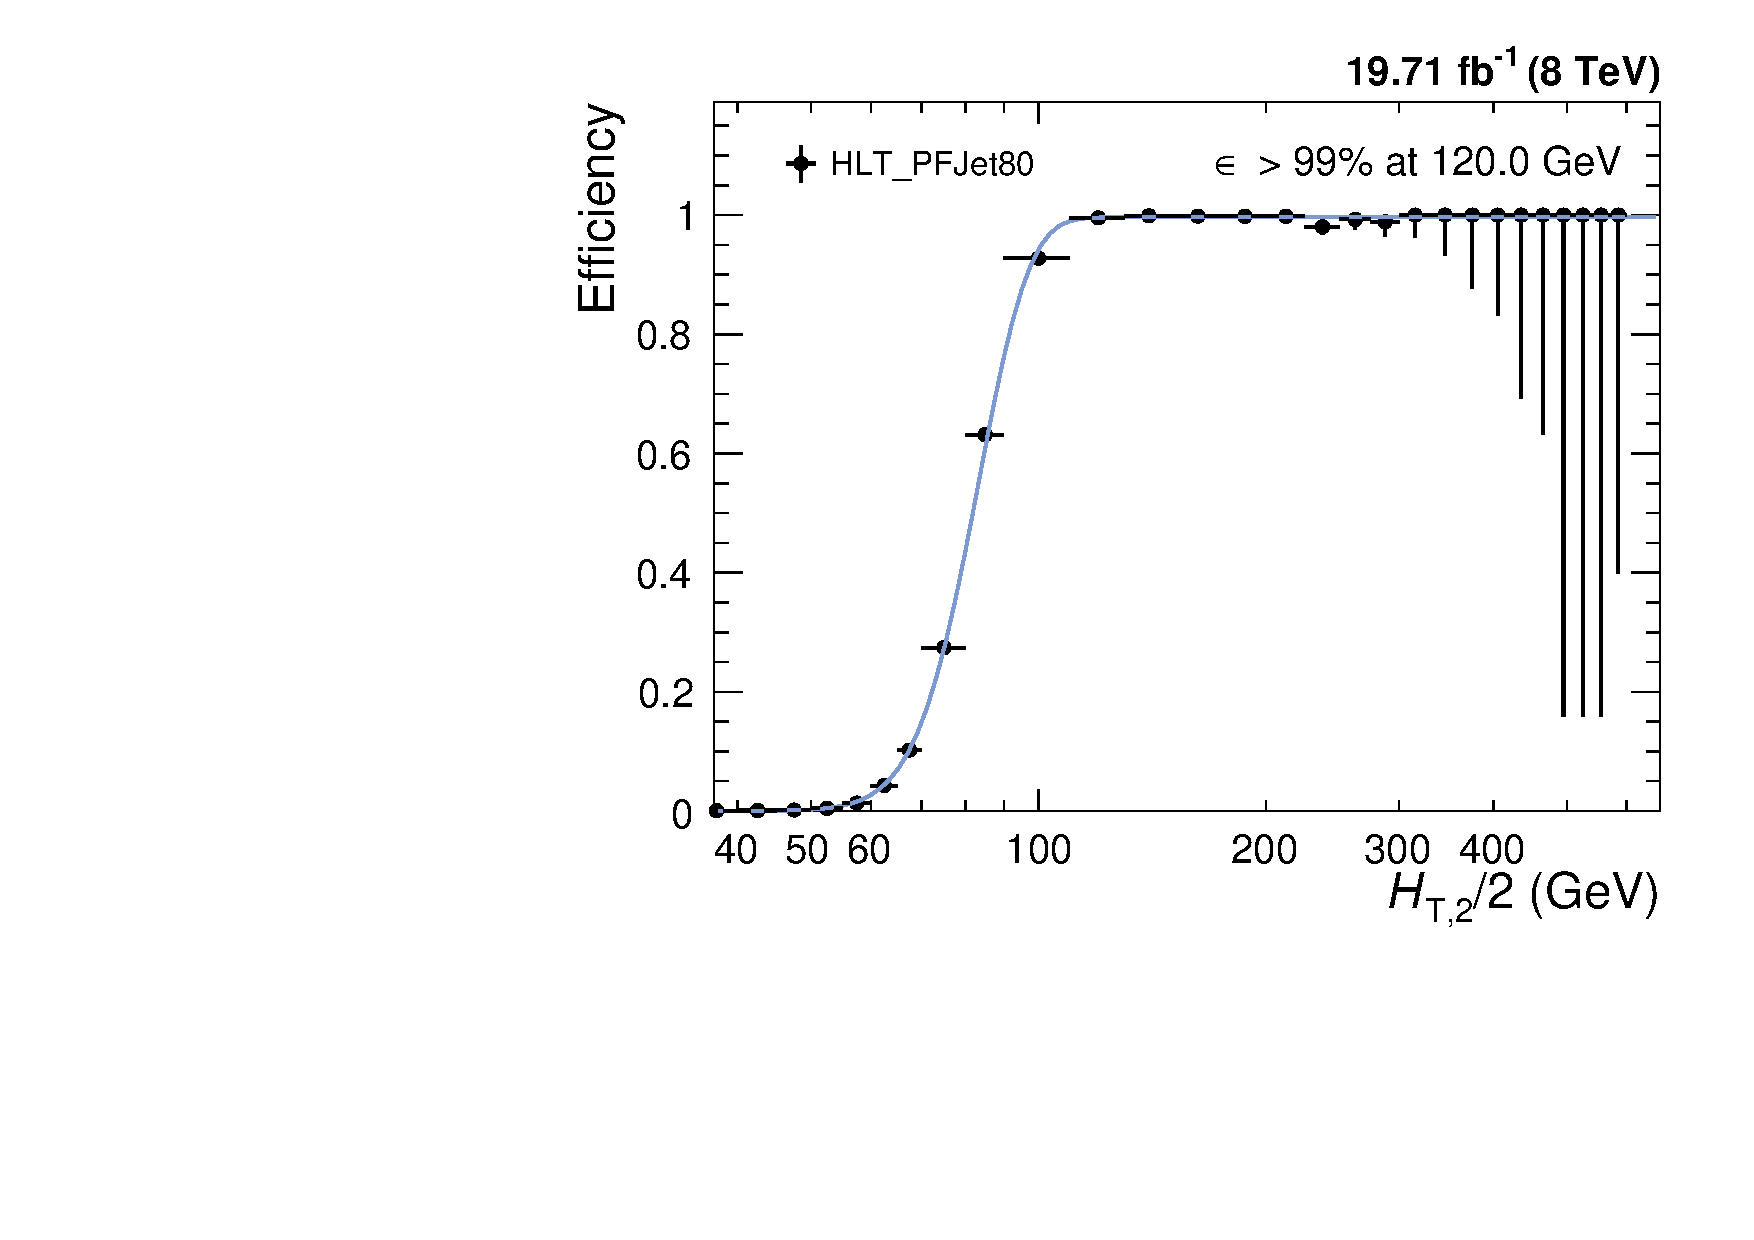
\includegraphics[width=0.53\textwidth]{Plots_HT_2_150/Fit_Turn_Efficiency_80_2_ht_2.pdf}%
 ~~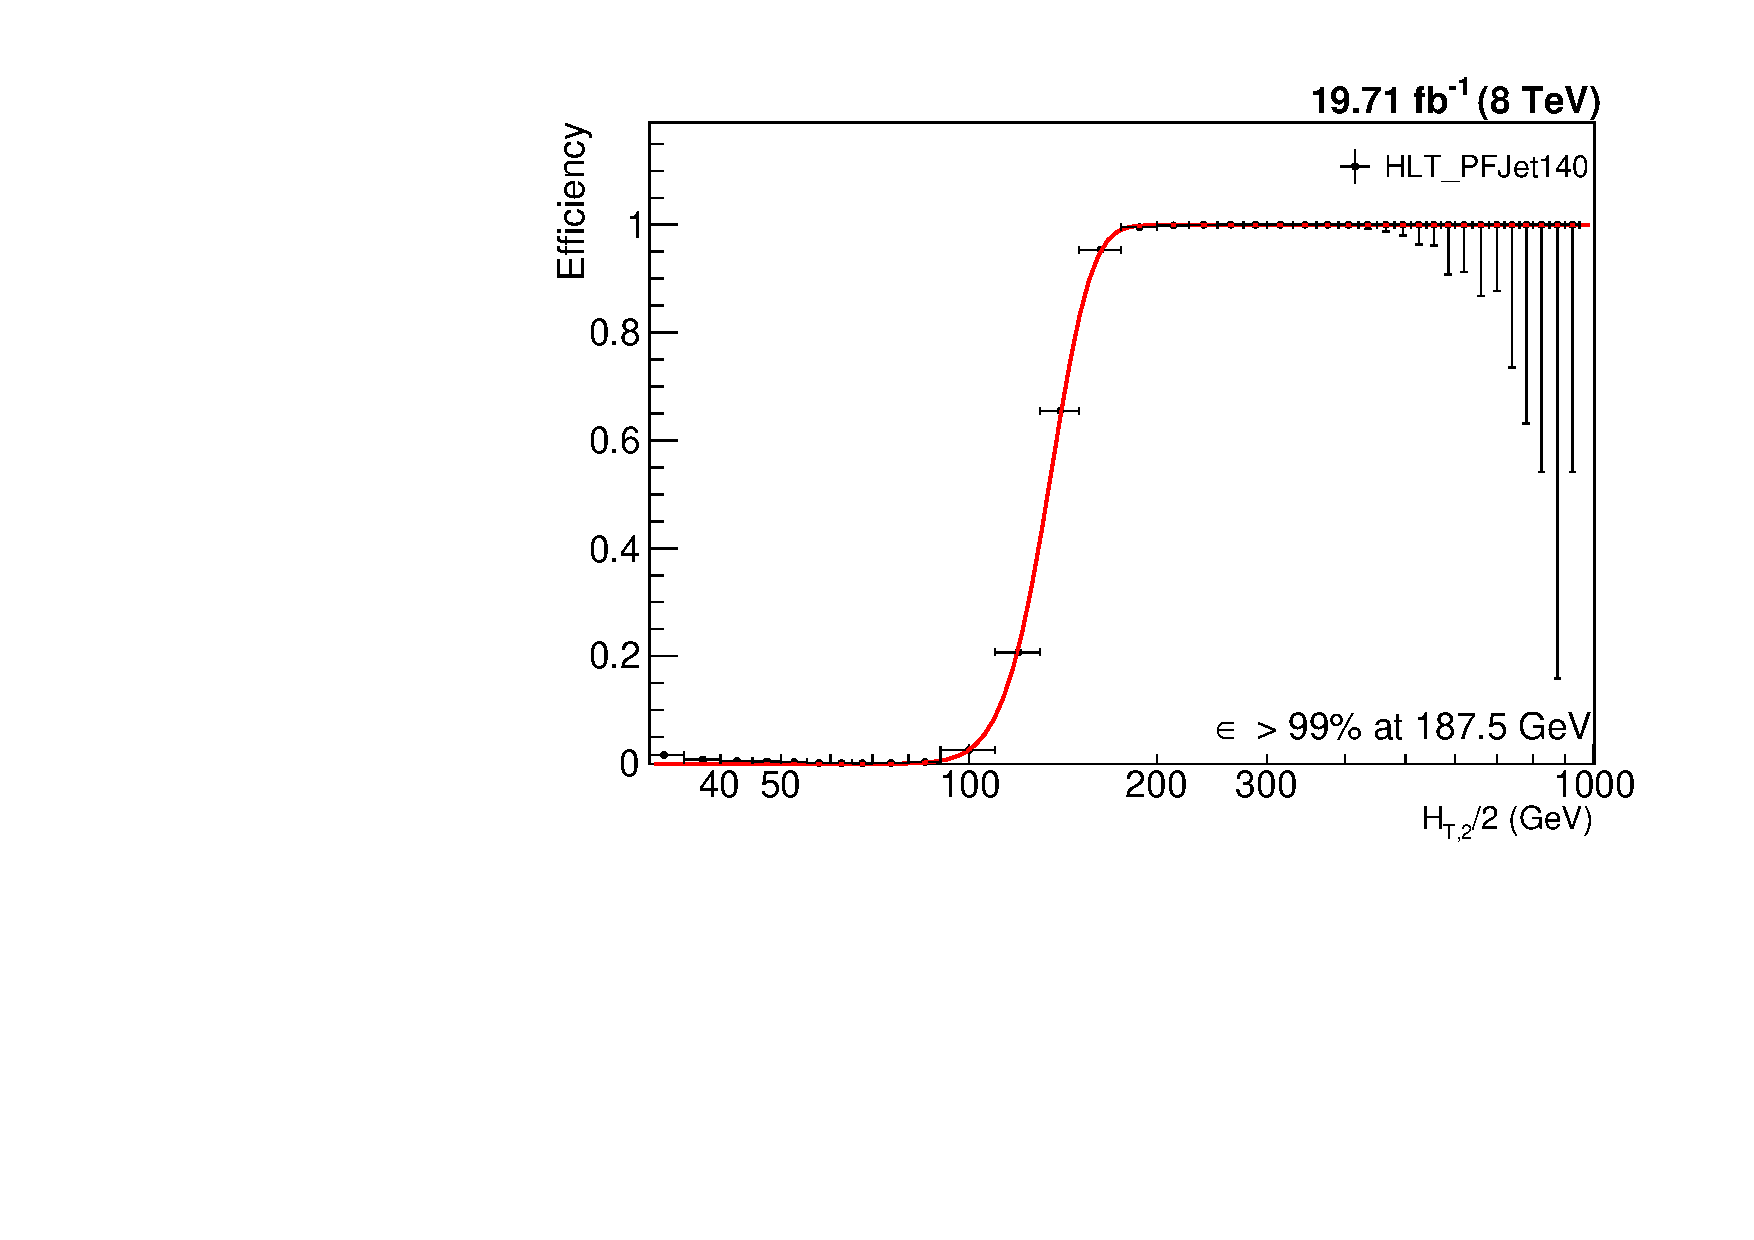
\includegraphics[width=0.53\textwidth]{Plots_HT_2_150/Fit_Turn_Efficiency_140_2_ht_2.pdf}\\
 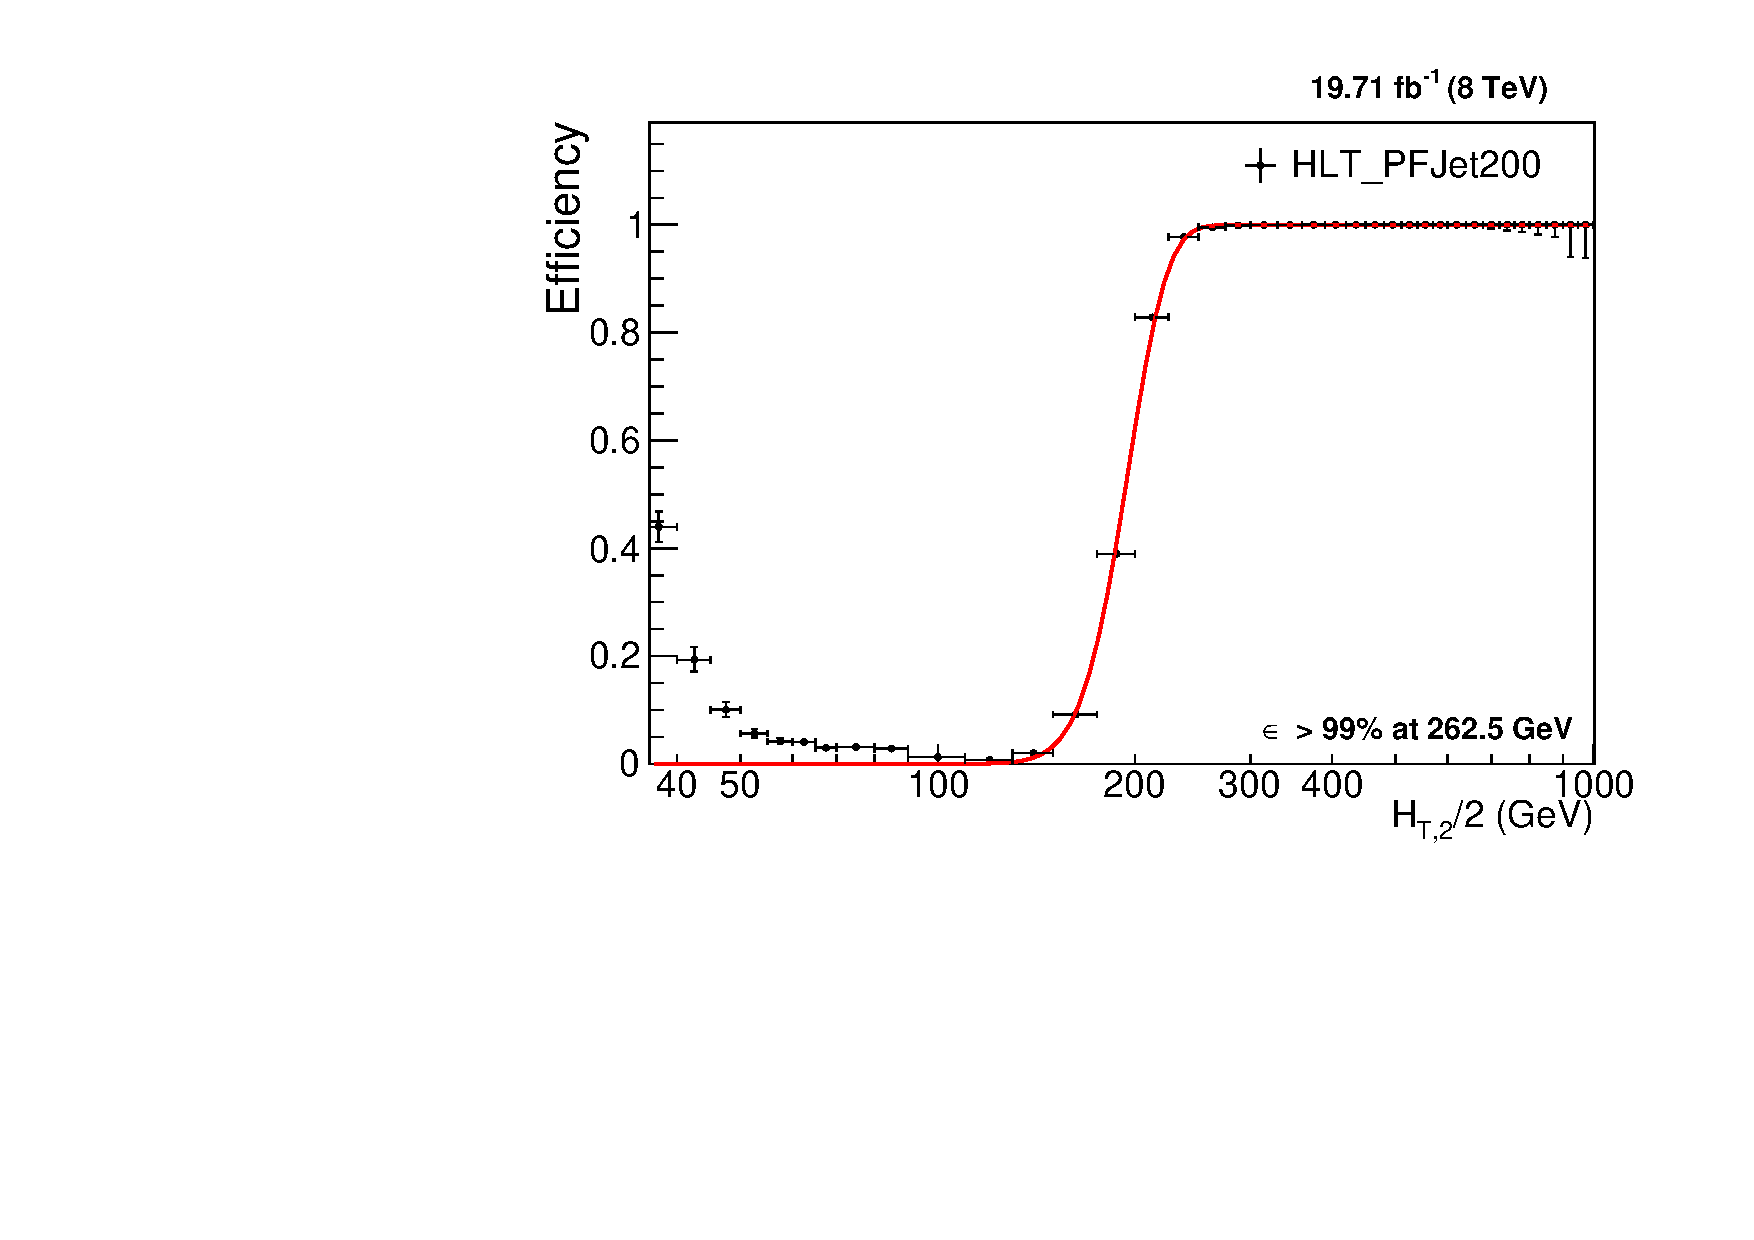
\includegraphics[width=0.53\textwidth]{Plots_HT_2_150/Fit_Turn_Efficiency_200_2_ht_2.pdf}%
 ~~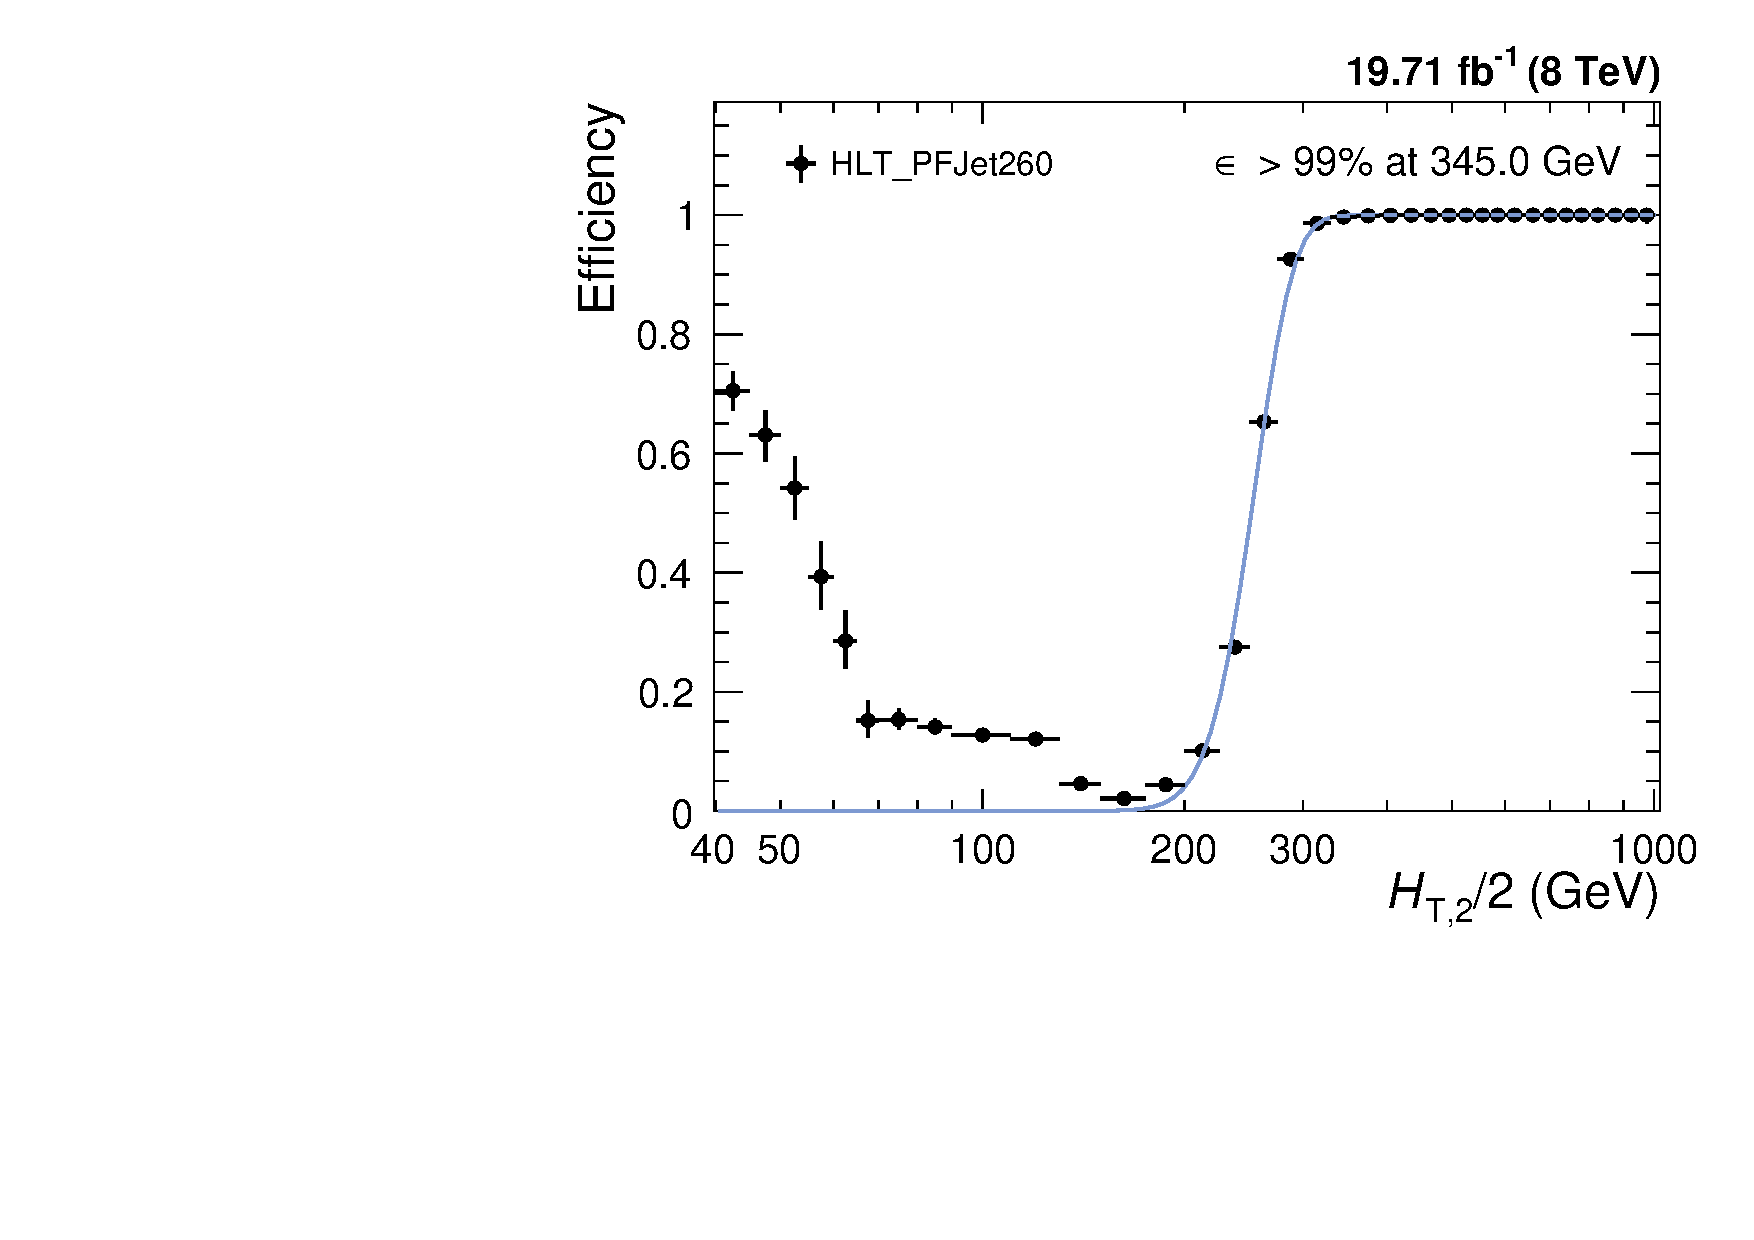
\includegraphics[width=0.53\textwidth]{Plots_HT_2_150/Fit_Turn_Efficiency_260_2_ht_2.pdf}\\
 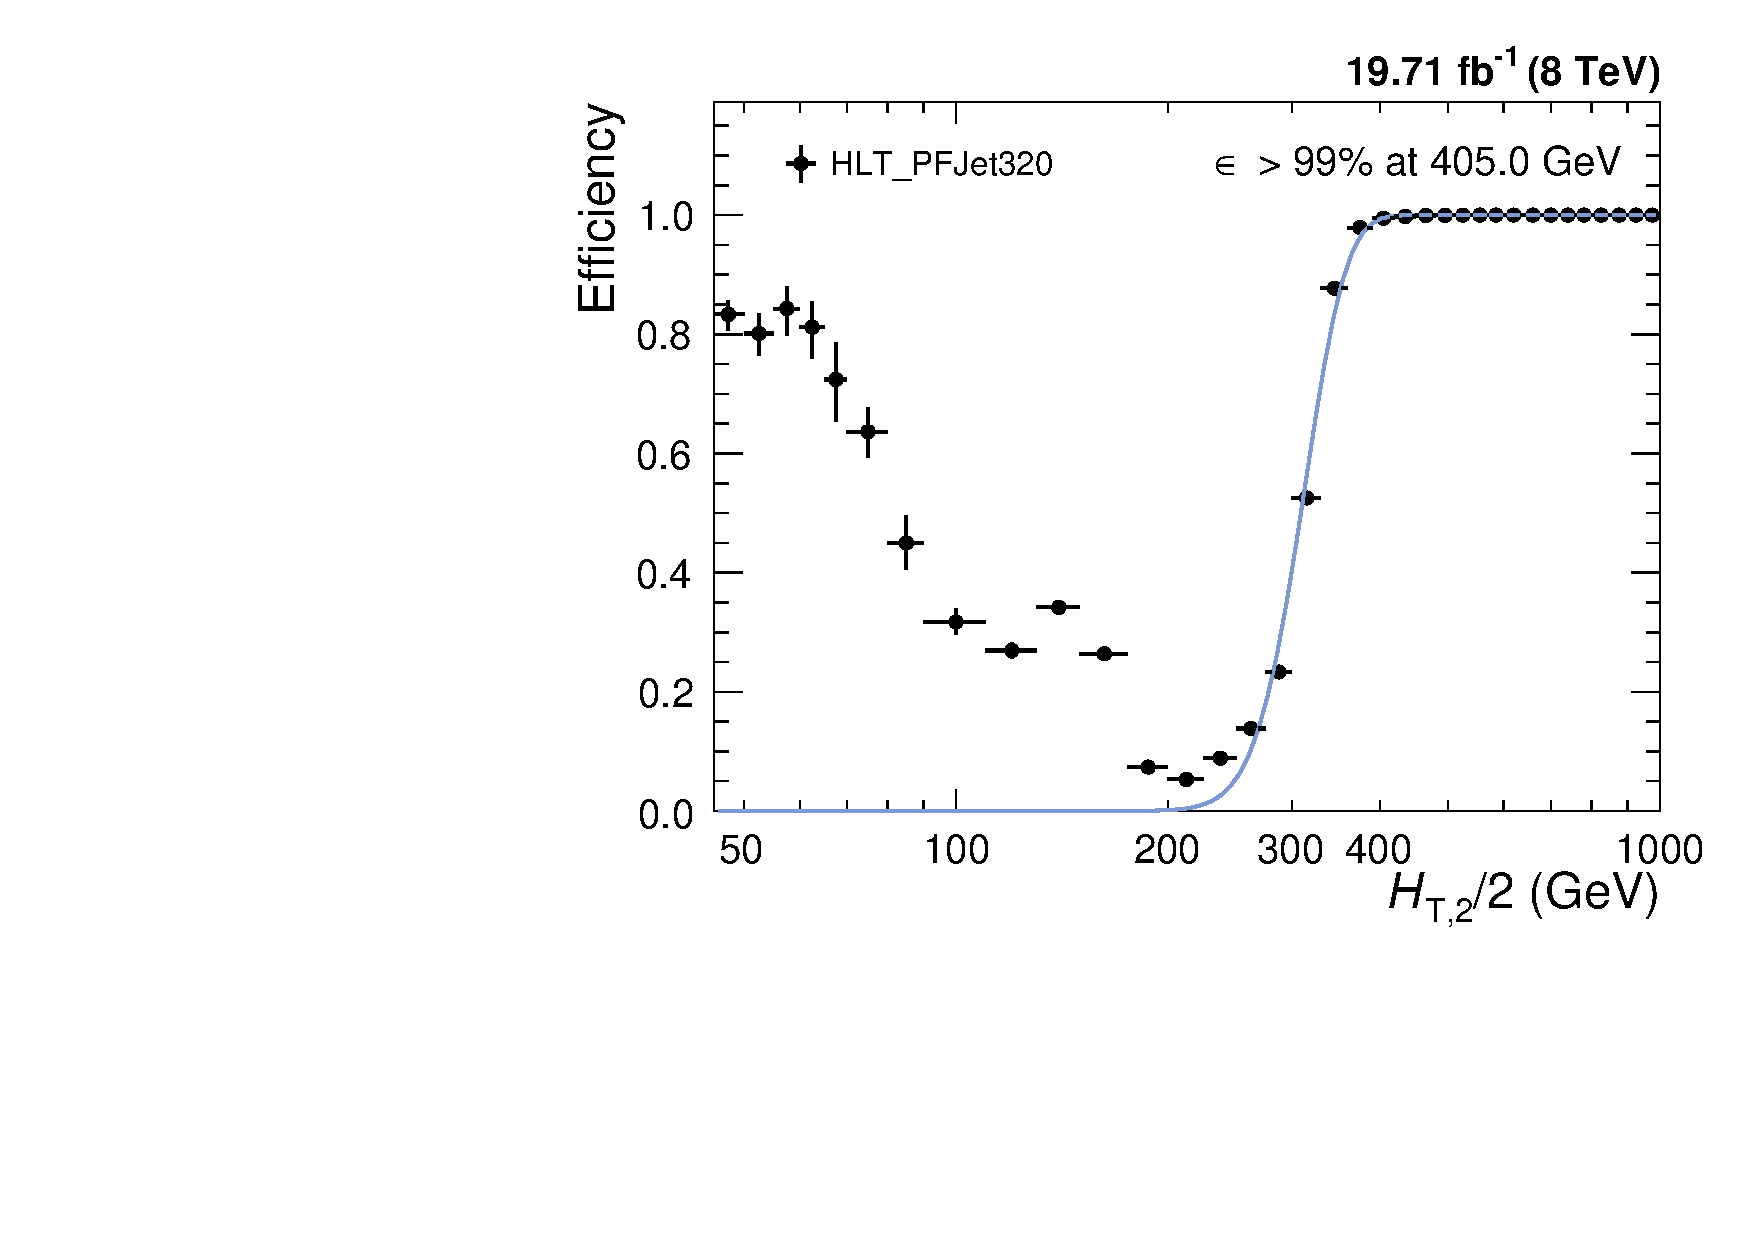
\includegraphics[width=0.53\textwidth]{Plots_HT_2_150/Fit_Turn_Efficiency_320_2_ht_2.pdf}%
 \caption{Trigger efficiencies turn-on curves for the single jet trigger paths used in the analysis. To determine the 99\% efficiency threshold, the trigger turn-on curves are fitted using a sigmoid function taking into account the uncertainties using Clopper-Pearson confidence intervals.}
 \label{fig:trig_eff}
 \end{center}
\end{figure}

\subsection{Primary Vertex Selection}
A primary vertex (PV) is identified by a collection of tracks, measured in the tracker with a good fit quality between the hits and compatible with the beam line. The tracks are clustered according to the z-coordinate of their point of closest approach to the beam axis. Each event is required to have at least one good PV which is well reconstructed within a distance of \abs{z(PV)}\ls 24 cm to the nominal interaction point of the detector. Also the radial distance in x-y plane, $\rho$(PV) should be smaller than 2 cm. The number of degrees of freedom in vertex fit needs to be at-least four. Thus, at least four tracks must be present in order to perform a valid vertex fit.

\subsection{Missing Transverse Energy}
If all particles could be identified and perfectly measured, the transverse momentum of all particles would sum up to zero. Neutral weakly interacting particles, such as neutrinos, escape from typical collider detectors without producing any direct response in the detector elements. The presence of such particles must be inferred from the imbalance of total momentum of all visible particles. The vector momentum imbalance in the plane perpendicular to the beam direction is known as missing transverse momentum or energy (\ETmiss). It is one of the most important observables for discriminating leptonic decays of W bosons and top quarks from background events which do not contain neutrinos, such  as multijet and Drell–Yan events or searches for physics beyond the Standard Model which involve undetectable particles.

The ratio of missing transverse energy to the total transverse energy \ETmiss/$\sum\ET$, shown in Fig.~\ref{fig:metcut} for \njt~(left) and \njth~(right), shows a discrepancy between data and MC at the tail part of the distribution. This is because of a  finite contribution from Z($\rightarrow \nu \bar{\nu}$) \plus jet events which gives rise to non-zero \ET in the events in data. Such events are absent in QCD simulated events in MC. Hence \ETmiss/$\sum\ET$ is required to be less than 0.3 to reject events with high \ETmiss.

\begin{figure}[!htbp]
\centering
 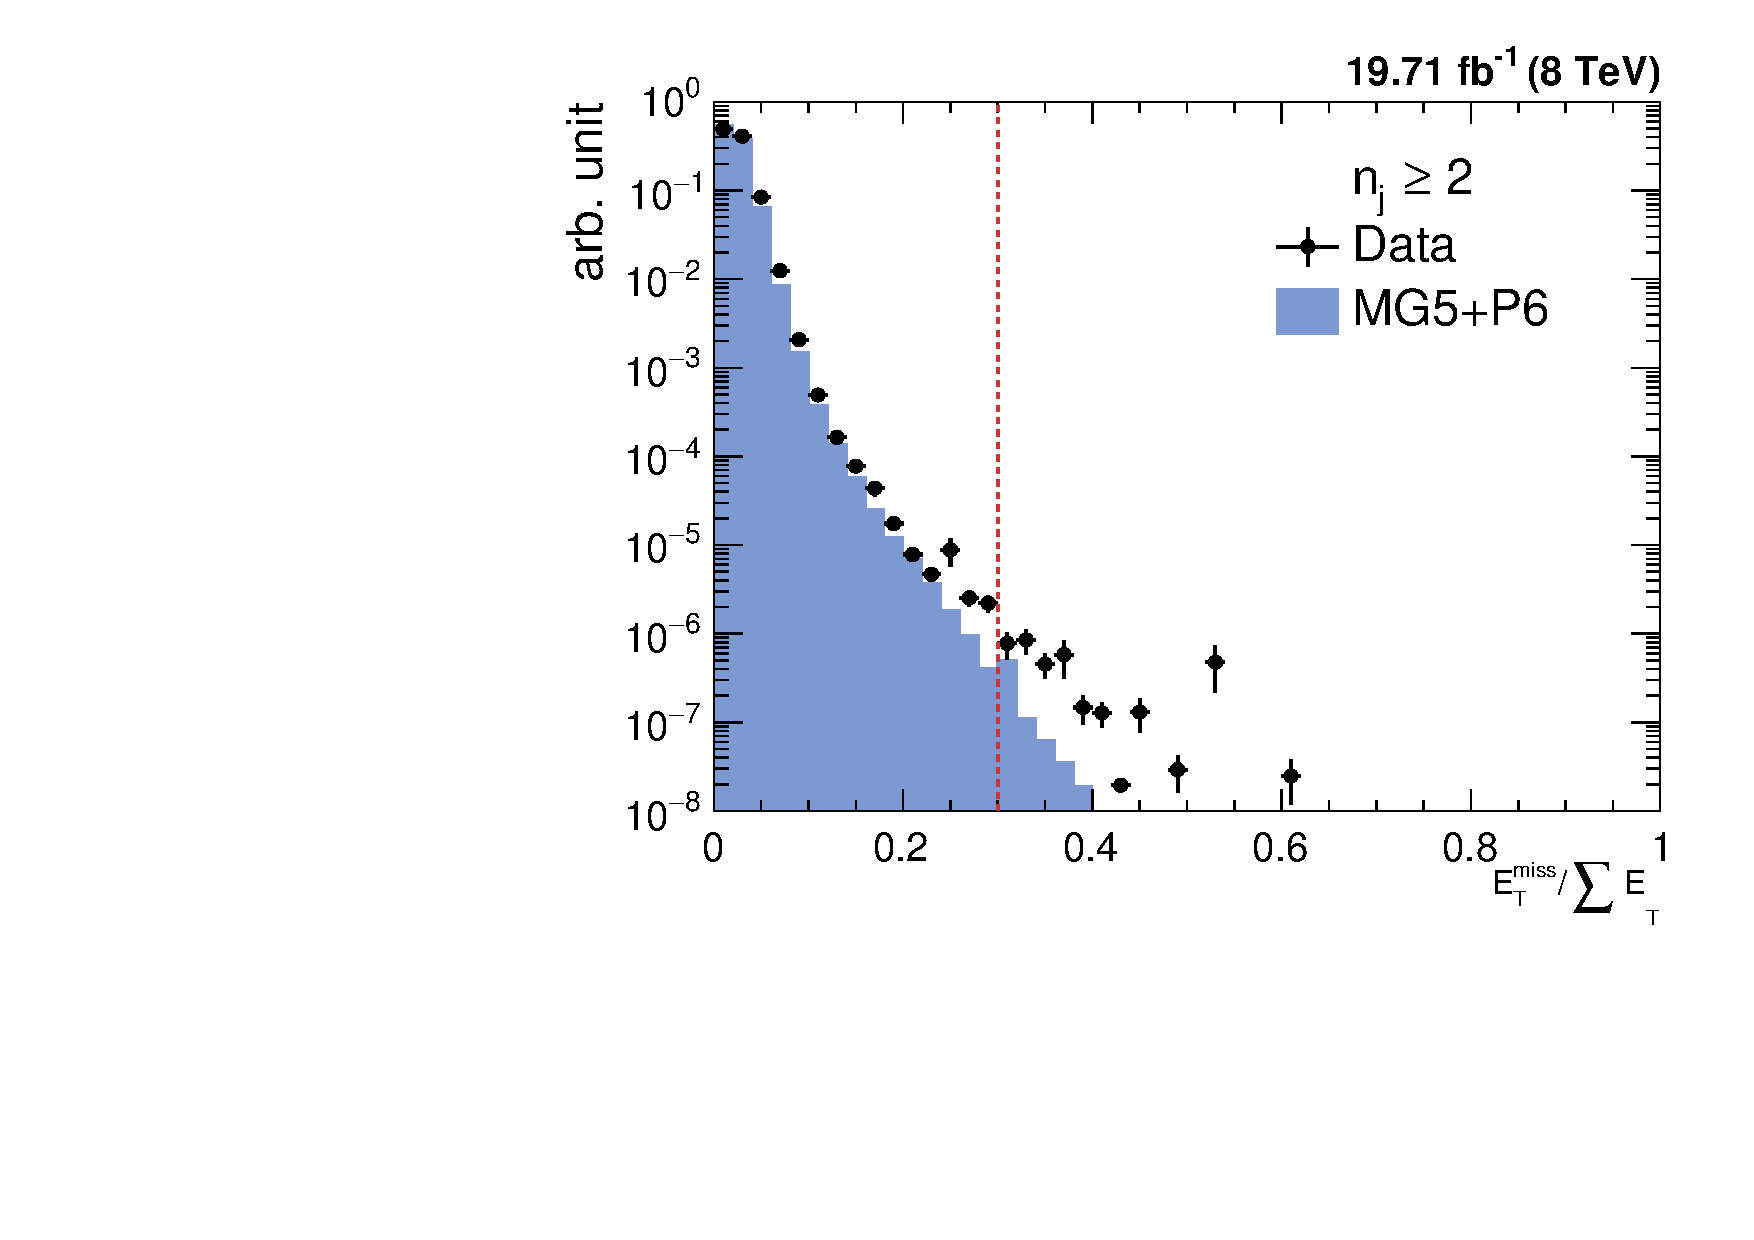
\includegraphics[width=0.51\textwidth]{Plots_HT_2_150/Missing_ET_2.pdf}%
 ~~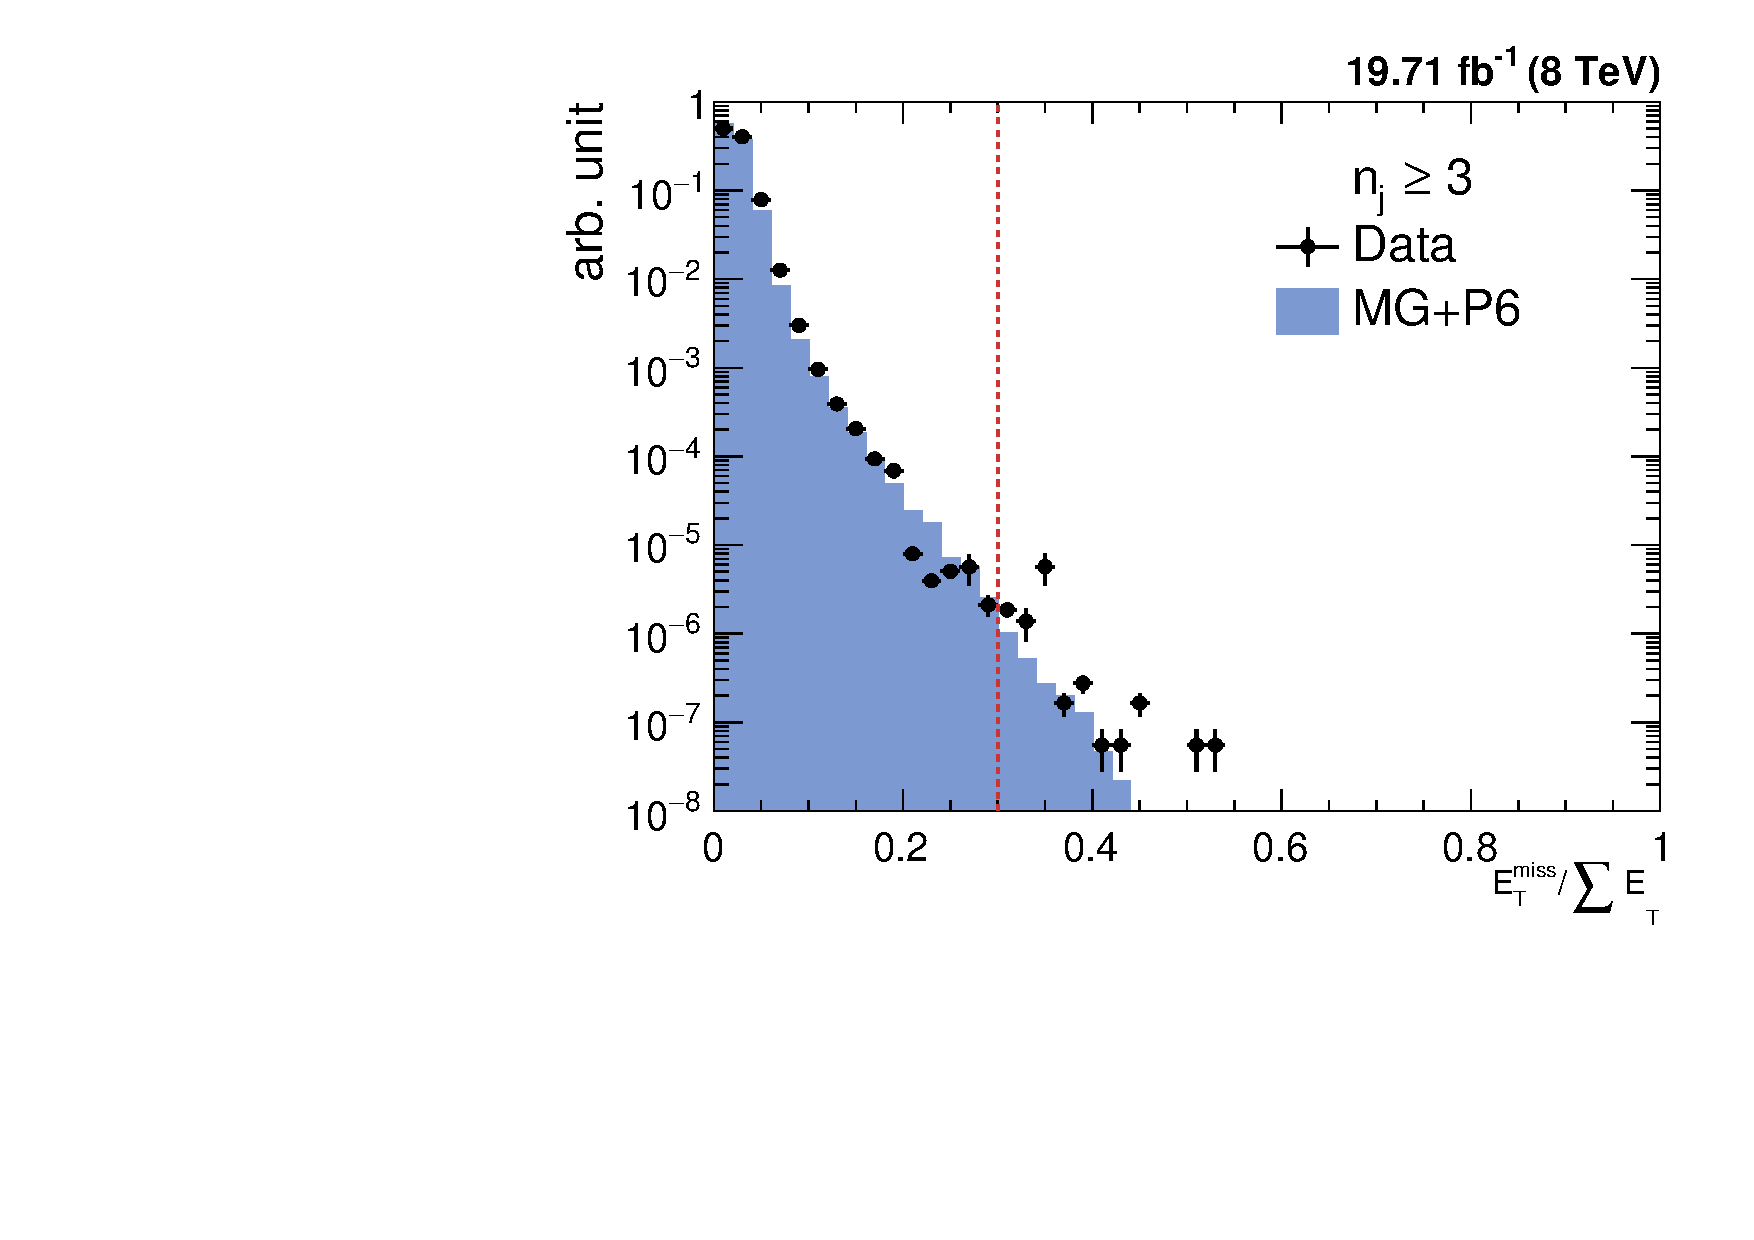
\includegraphics[width=0.51\textwidth]{Plots_HT_2_150/Missing_ET_3.pdf}
 \caption{Missing transverse energy fraction of the total transverse energy per event in data and simulated events in inclusive 2-jet (left) and 3-jet events (right). To remove background and noise, events with a fraction exceeding a certain threshold, here indicated with the red dashed line, are rejected.}
 \label{fig:metcut}
\end{figure} 

\subsection{Jet Identification}
In order to suppress fake jets, arising from detector noise or misreconstructed particles, jet identification criteria (ID) has been applied. Instead of applying it event-wise, it  is applied it on each jet. The algorithm works on reconstructed jets using information of the clustered particle candidates. The official tight jet ID \cite{CMS:2010xta}, recommended by \JetMet group \cite{JetID} is used. Due to pileup and electronic noise the jet constituent fractions may vary from event to event. In order to reject the noisy jets, some jet selection criteria are optimized to select only good quality jets. The selection criteria are implemented as selection cut on jet fractions. Table~\ref{tab:jetID} summarizes the properties of the reconstructed jets and their respective cuts. Each jet should contain at least two particles, one of which should be a charged hadron. The cut on the fraction of neutral hadrons and photons removes HCAL noise and ECAL noise, respectively. Muons that are falsely identified and clustered as jets are removed by the muon fraction criterion. Based on information of the tracker, additional selection cuts are enforced in the region $|\eta|$ \ls 2.4. The charged electromagnetic fraction cut removes the jets clustered from misidentified electrons. Furthermore, the fraction of charged hadrons in the jet must be larger than zero and jets without any charged hadrons are very likely to be pileup jets. The Figures~\ref{fig:qual2} and~\ref{fig:qual3} show the distributions of the jet constituents observed in data and simulated events for \njt~and \njth, respectively.

\begin{table}[!htbp]
 \centering
 \caption{The jet ID removes noise and fake jets based on the properties of the reconstructed jets and the clustered particle candidates. All the selection cuts which are recommended by the \JetMet group are applied \cite{JetID}.}
 \label{tab:jetID}
 \vspace{2mm}
 \begin{tabular}{cccc}
 \hline\hline
 \centering
  & {\bf Property} & {\bf ~~~Loose ID} & {\bf ~~~Tight ID} \rbthm\\\hline
  & neutral hadron fraction  & ~~~\ls 0.99 & ~~~\ls 0.90 \rbtrr \\
 Whole & neutral EM fraction & ~~~\ls 0.99 & ~~~\ls 0.90 \rbtrr \\
 $\eta$ region  & number of constituents  & \gr 1    & \gr 1    \rbtrr \\
  & muon fraction           & ~~~\ls 0.80 & ~~~\ls 0.80 \rbtrr \\ \hline
  & charged hadron fraction & \gr 0    & \gr 0    \rbtrr \\
  only $|\eta|$ \ls 2.4 & charged multiplicity    & \gr 0    & \gr 0    \rbtrr \\
  & charged EM fraction     & ~~~\ls 0.99 & ~~~\ls 0.90 \rbtrr \\
 \hline\hline
  \end{tabular}
\end{table}

\begin{figure}[!htbp]
 \begin{center}
 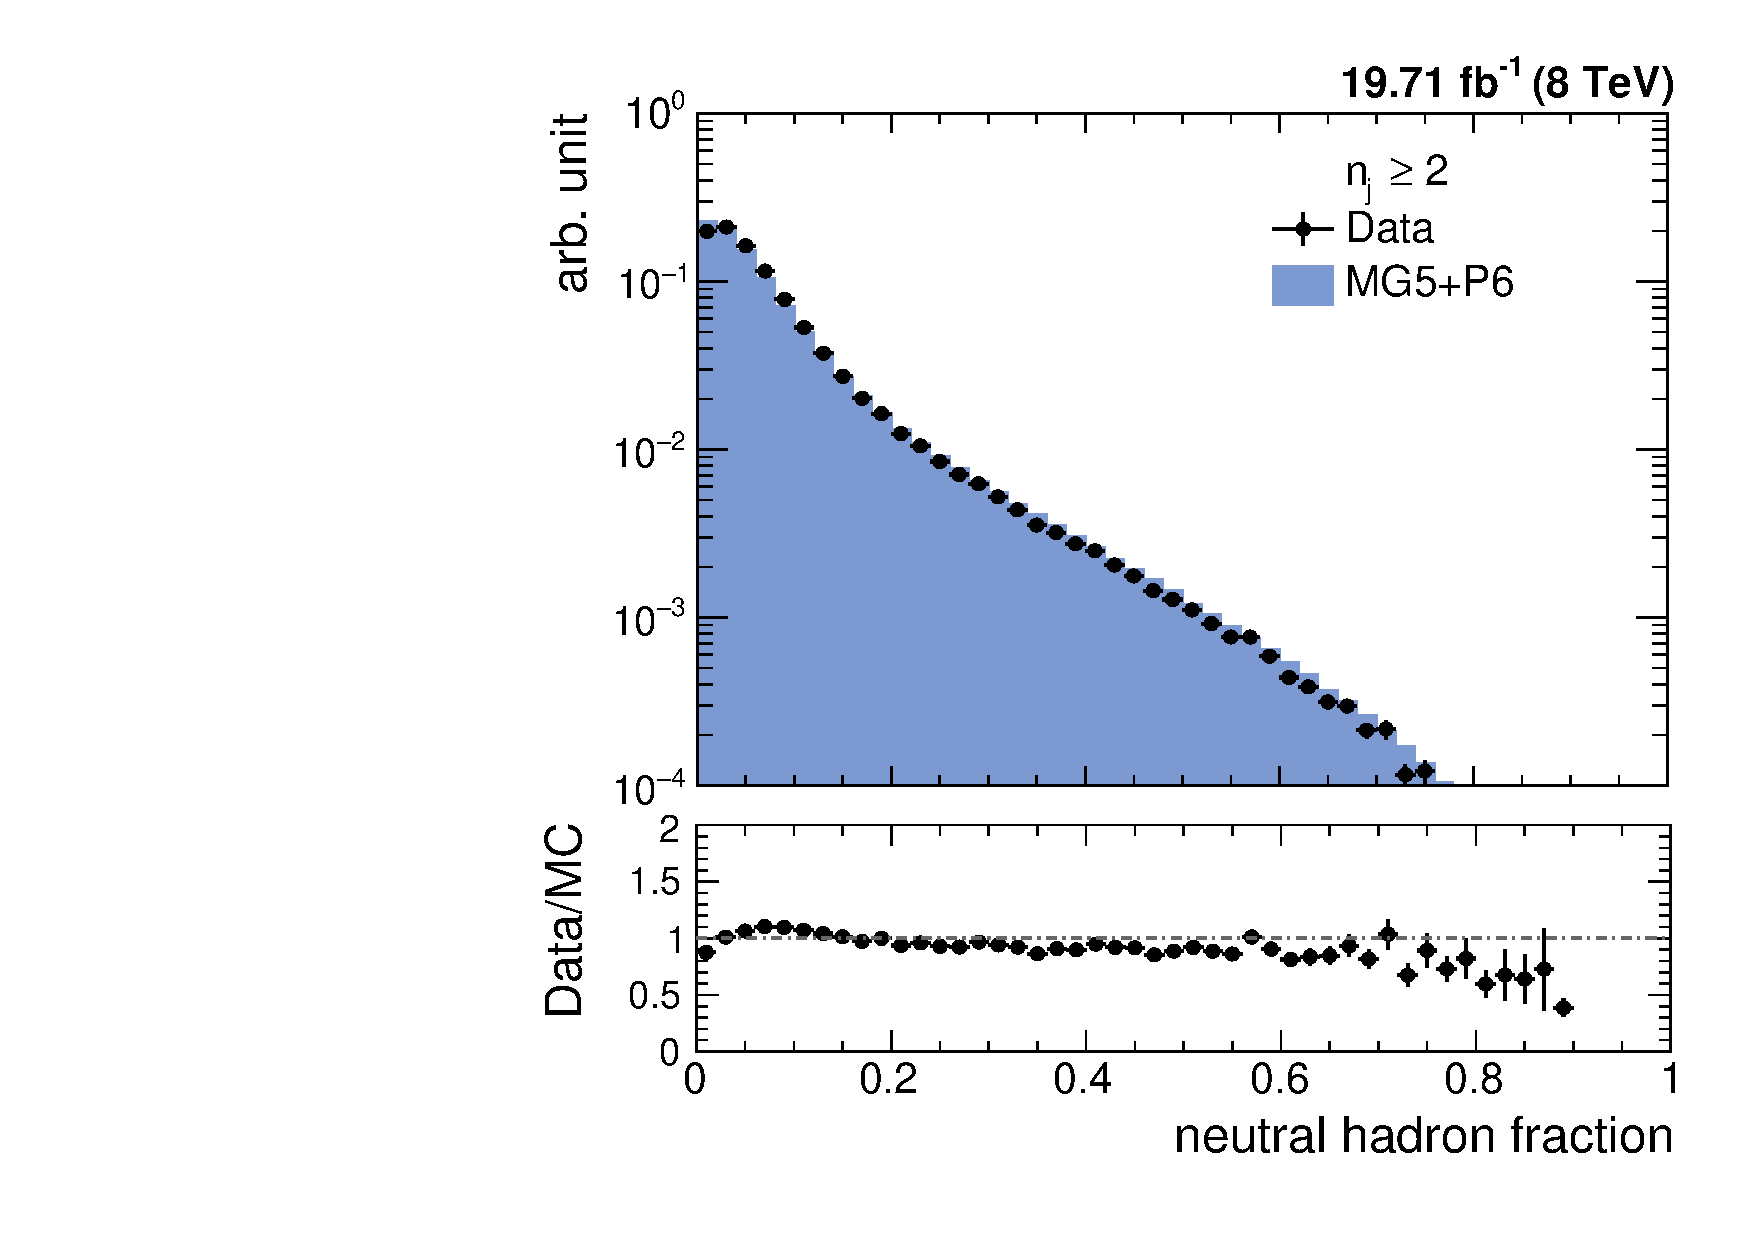
\includegraphics[width=0.5\textwidth]{Plots_HT_2_150/Comparison_NuHadFrac_2_HT_2_150.pdf}%
 ~~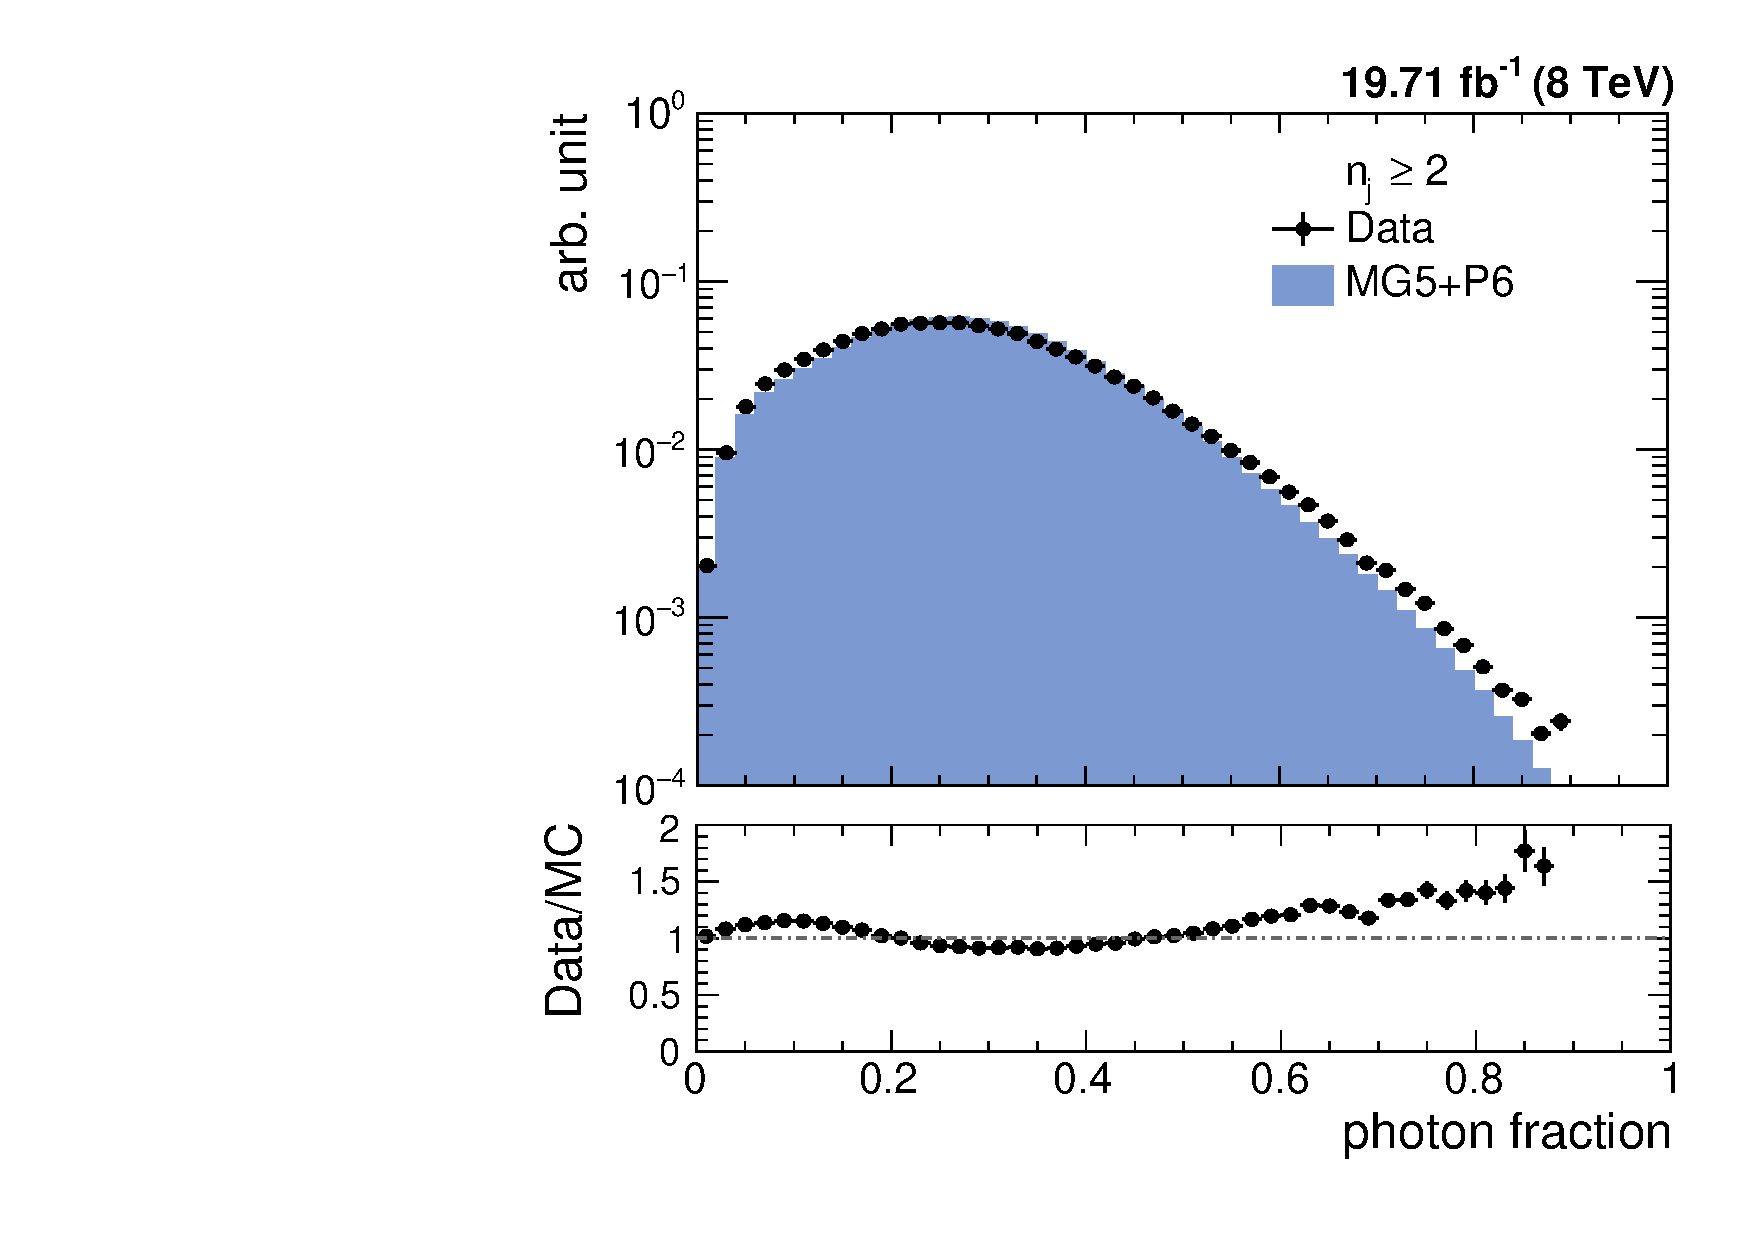
\includegraphics[width=0.5\textwidth]{Plots_HT_2_150/Comparison_PhFrac_2_HT_2_150.pdf}\\
 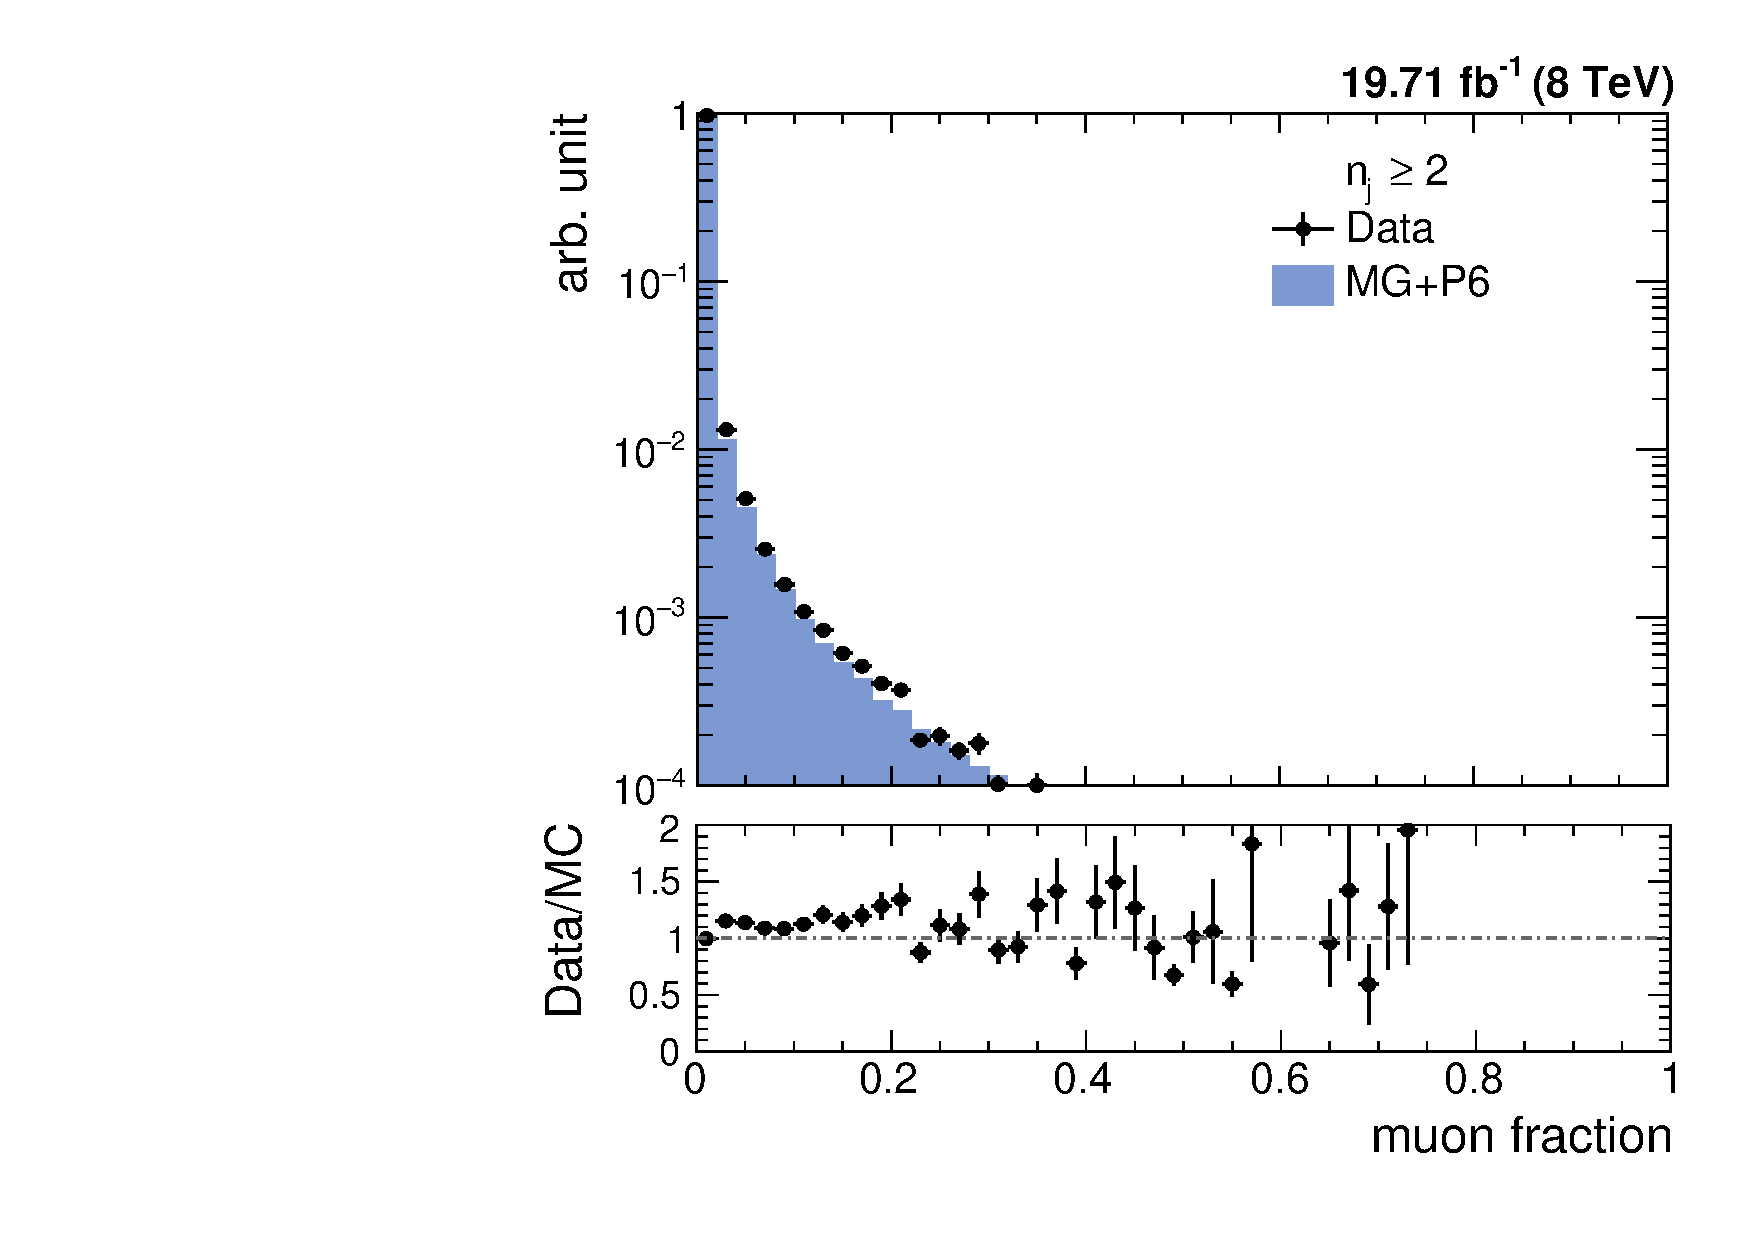
\includegraphics[width=0.5\textwidth]{Plots_HT_2_150/Comparison_MuFrac_2_HT_2_150.pdf}%
 ~~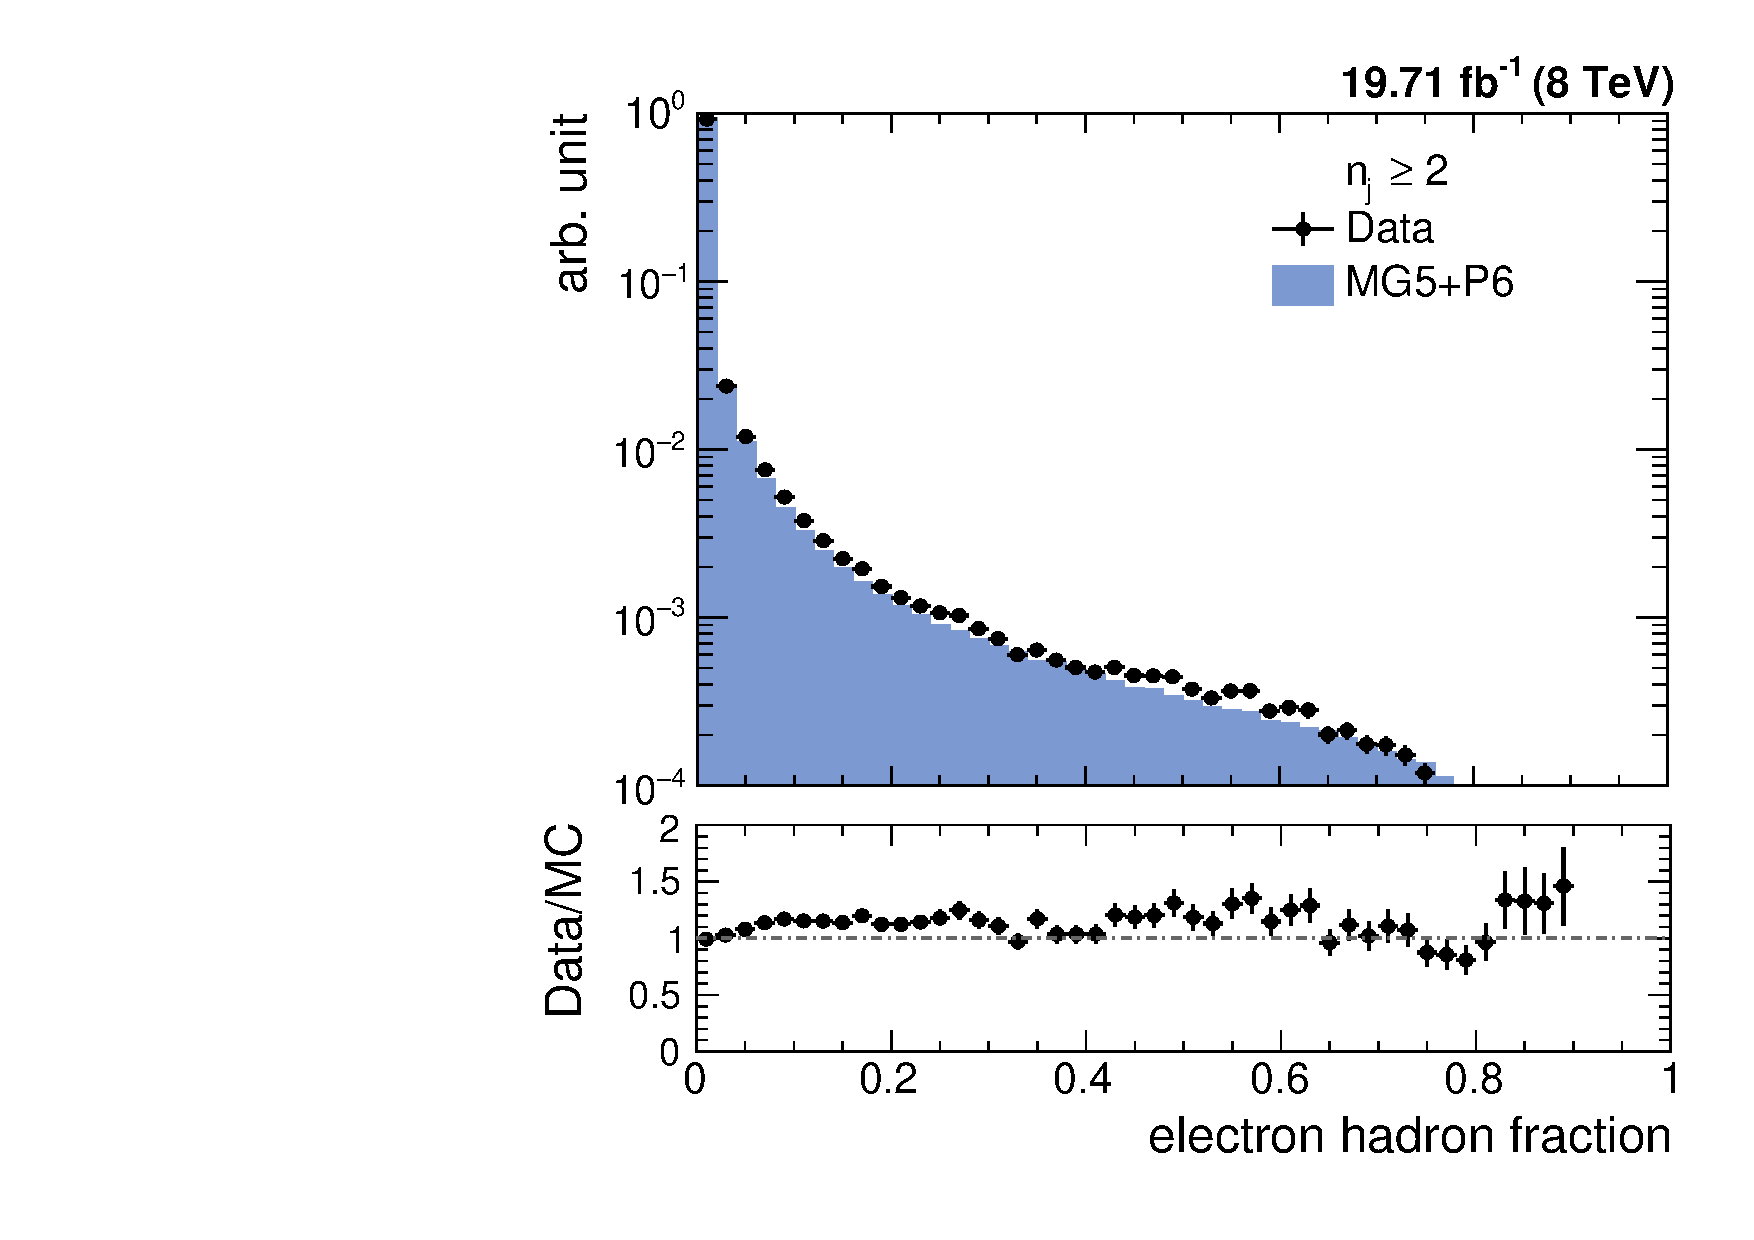
\includegraphics[width=0.5\textwidth]{Plots_HT_2_150/Comparison_ElFrac_2_HT_2_150.pdf}\\
 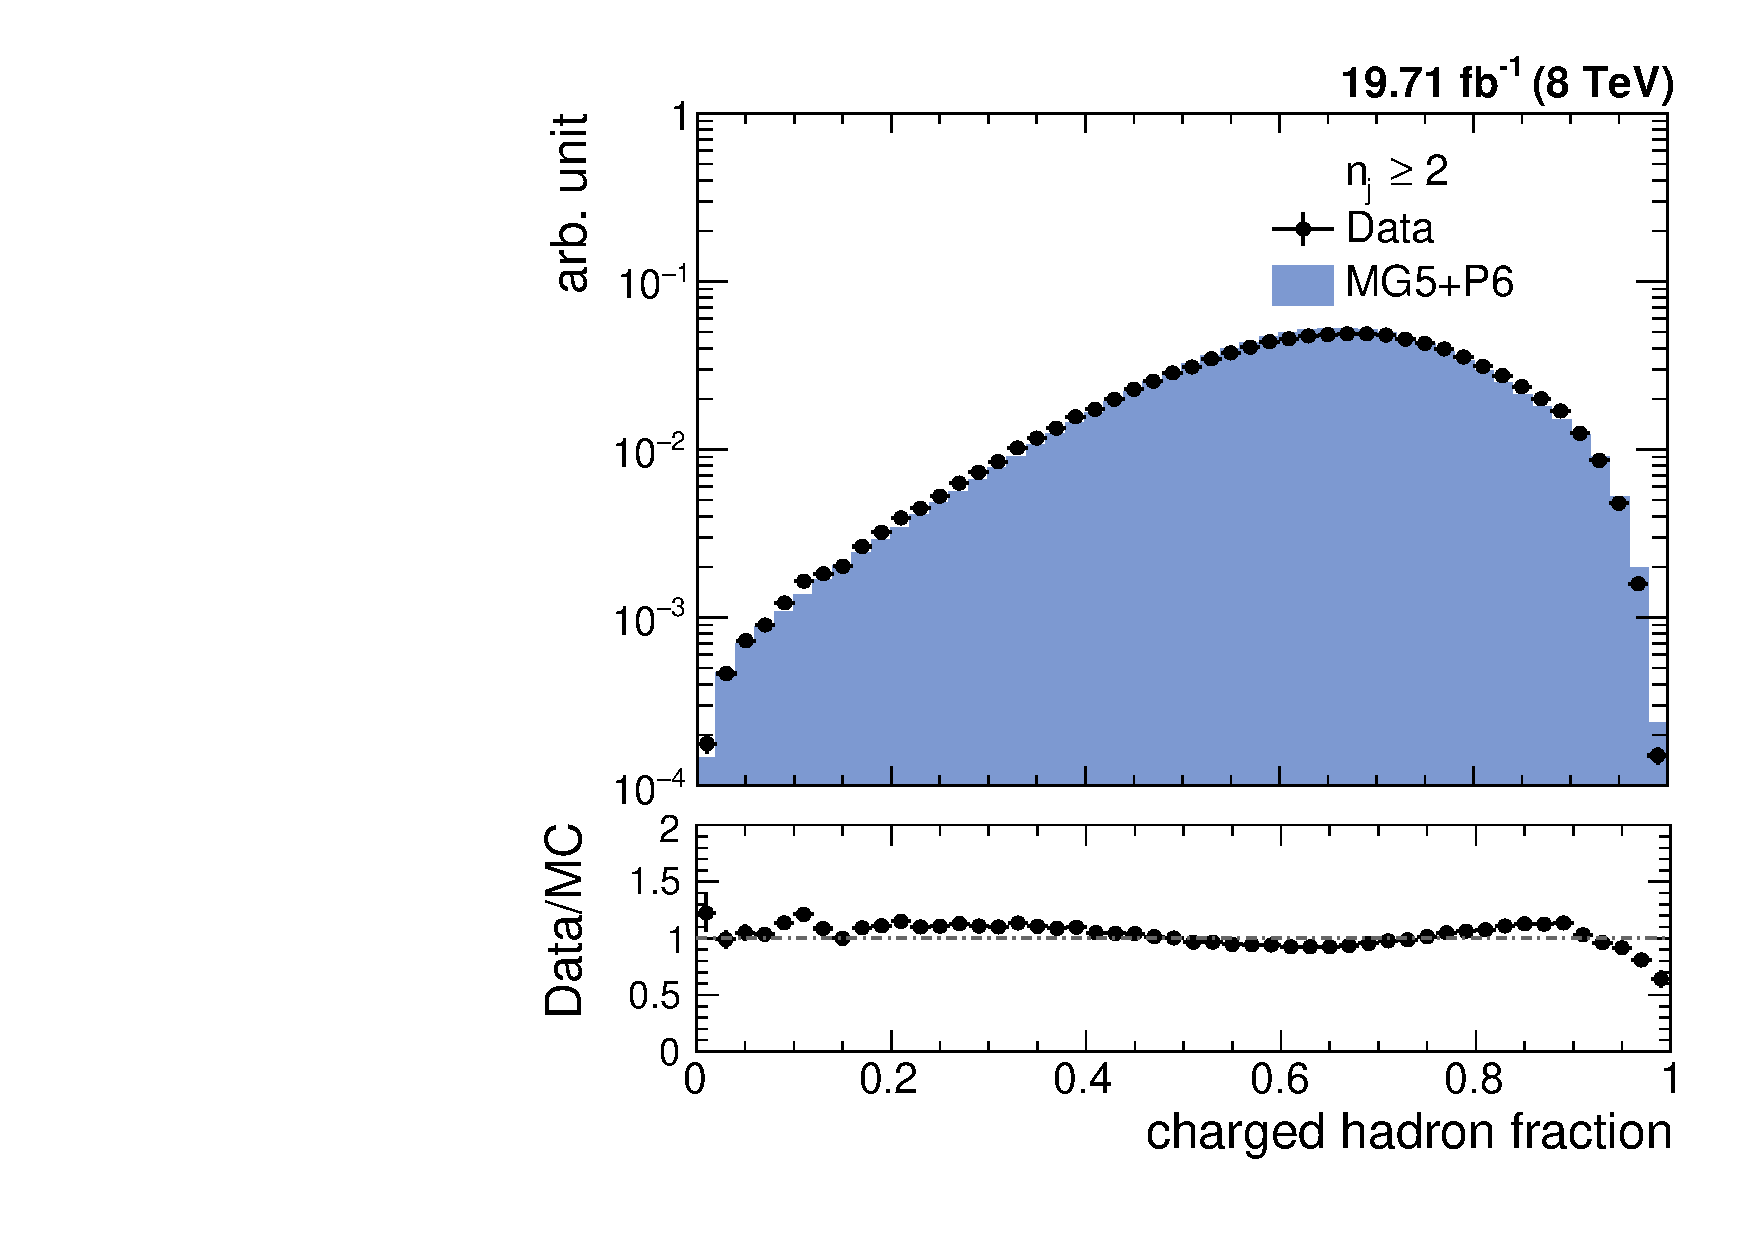
\includegraphics[width=0.5\textwidth]{Plots_HT_2_150/Comparison_ChHadFrac_2_HT_2_150.pdf}%
 \caption{The fractions of jet constituents as observed in data and simulated events for different types of PF candidates for inclusive 2-jet events. Data and simulation are normalized to the same number of events. The distributions are shown after the application of the jet ID.}
 \label{fig:qual2}
 \end{center}
\end{figure} 

\begin{figure}[!htbp]
 \begin{center}
 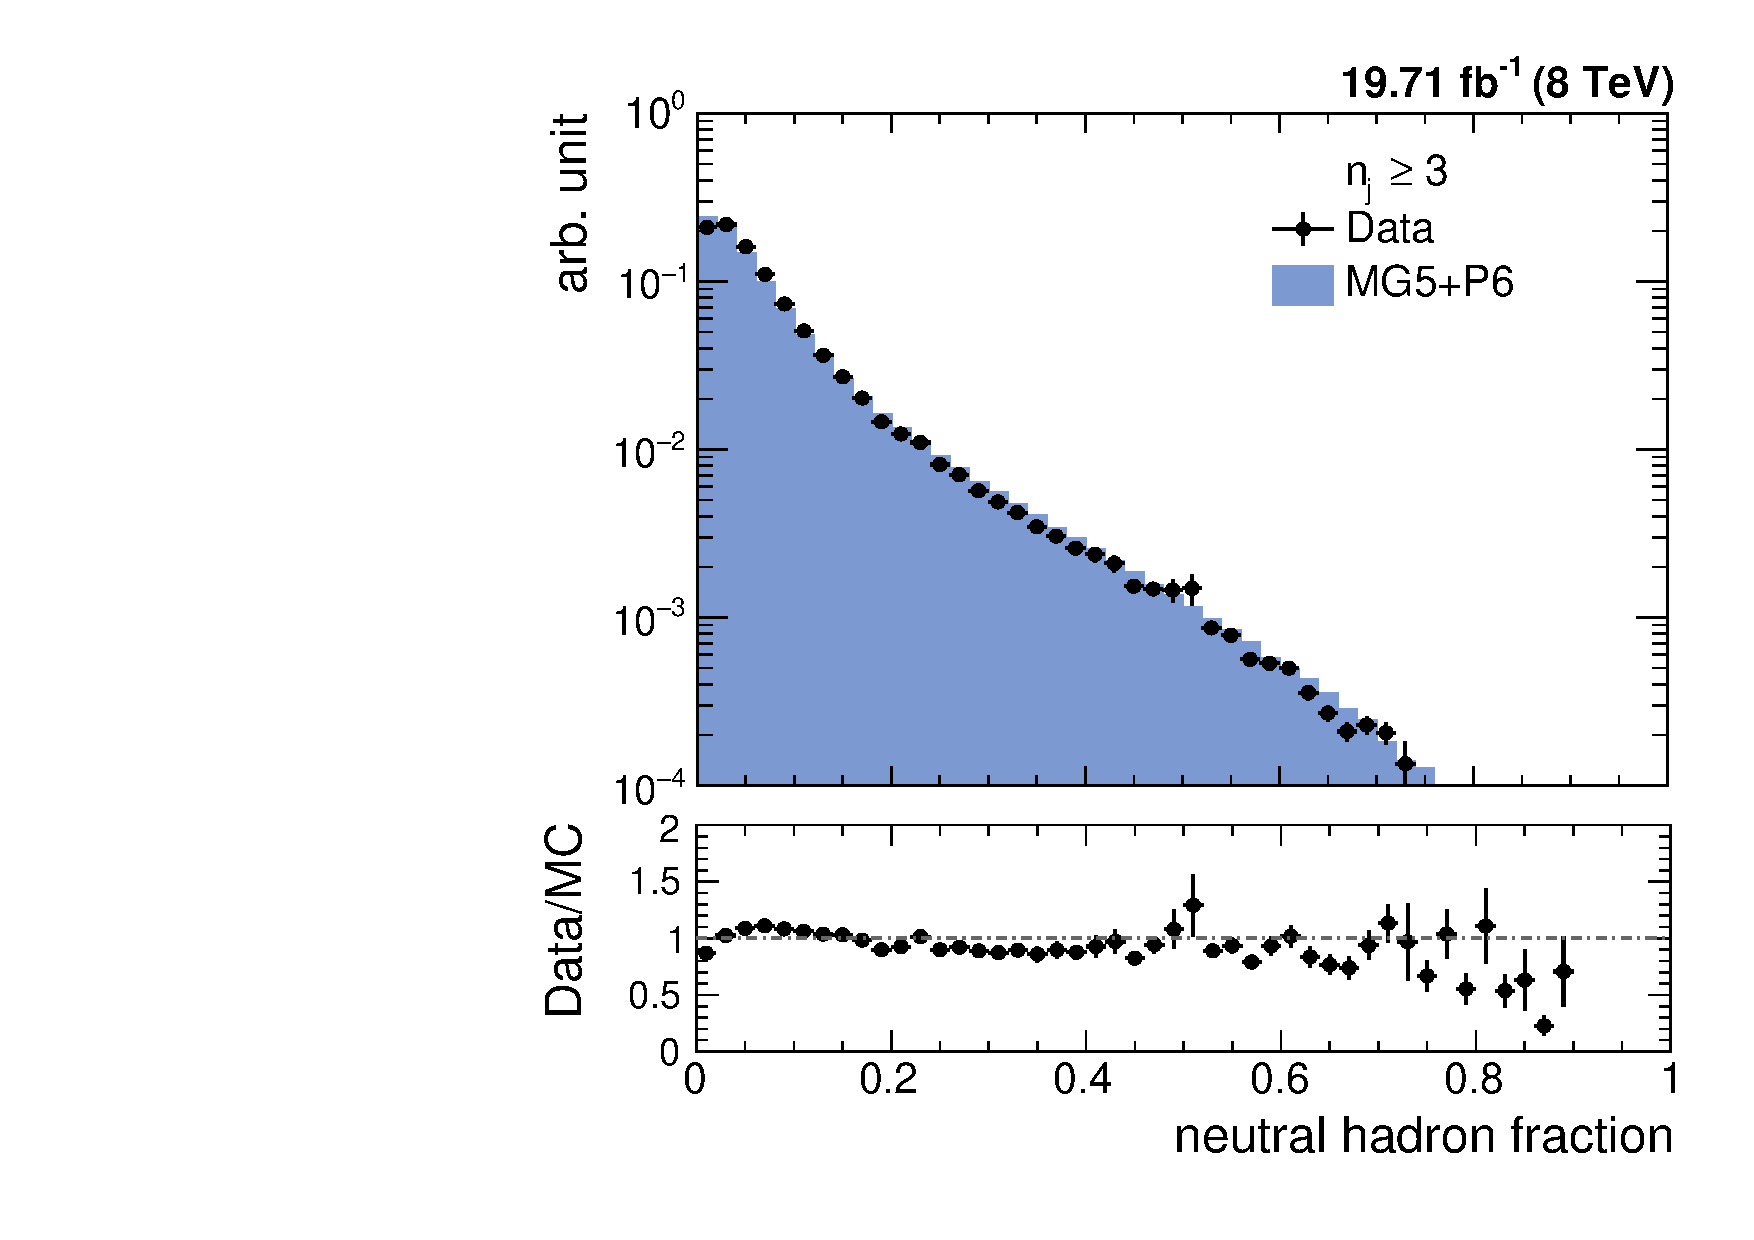
\includegraphics[width=0.5\textwidth]{Plots_HT_2_150/Comparison_NuHadFrac_3_HT_2_150.pdf}%
 ~~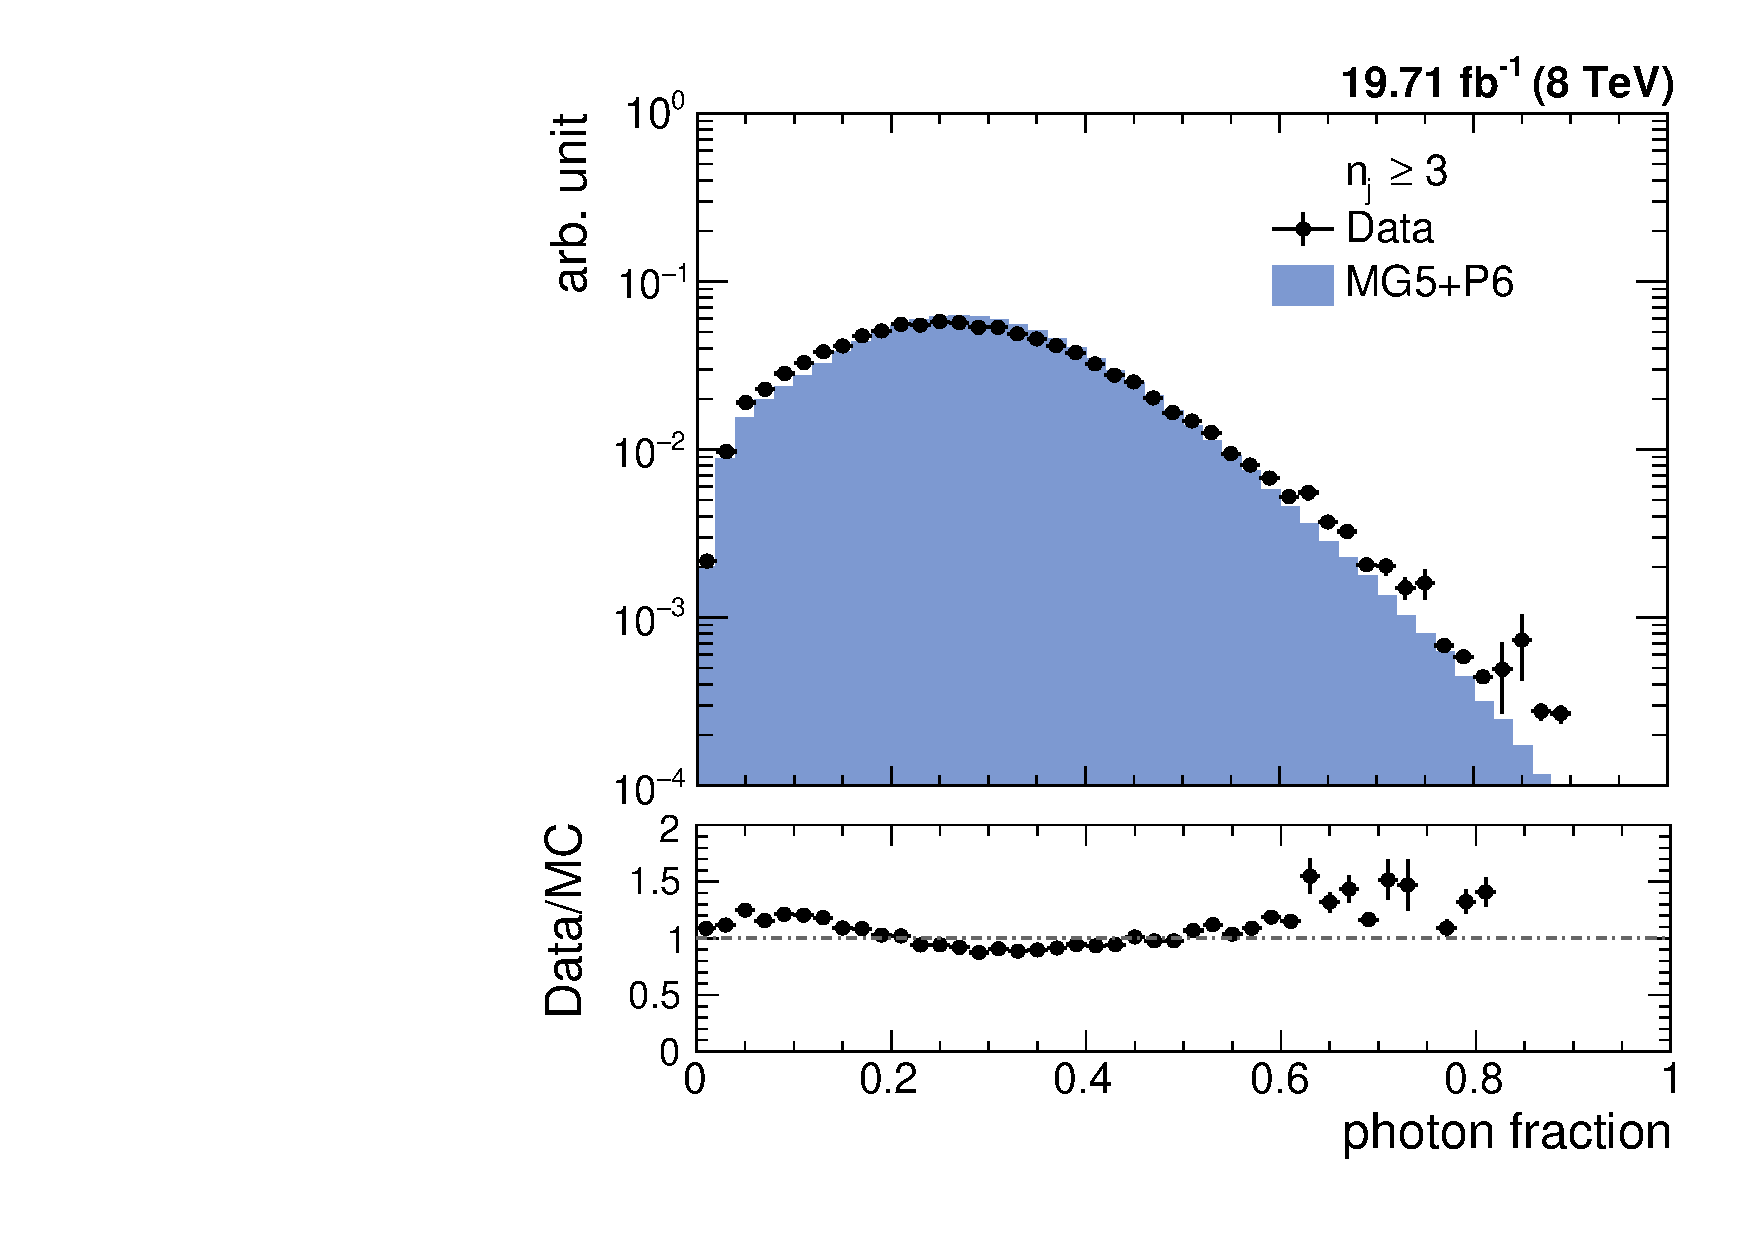
\includegraphics[width=0.5\textwidth]{Plots_HT_2_150/Comparison_PhFrac_3_HT_2_150.pdf}\\
 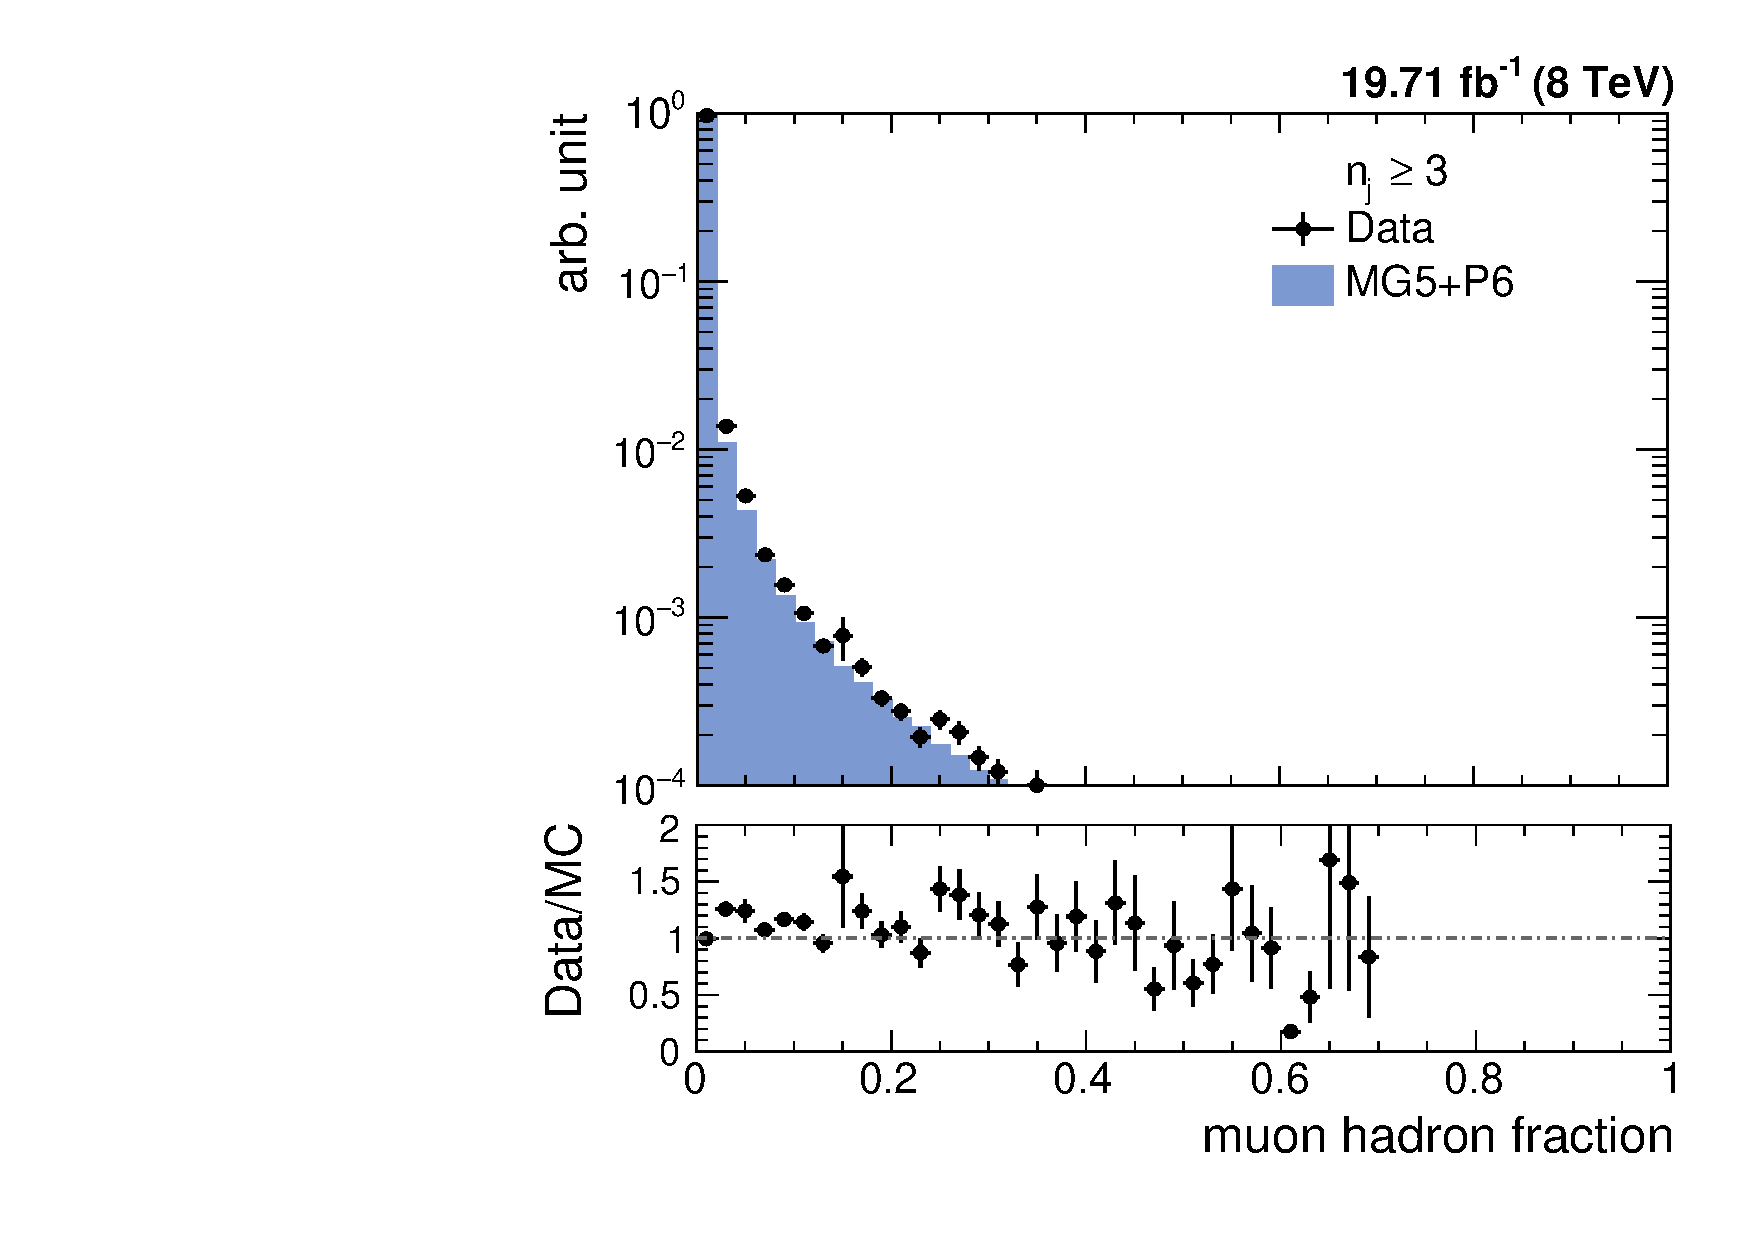
\includegraphics[width=0.5\textwidth]{Plots_HT_2_150/Comparison_MuFrac_3_HT_2_150.pdf}%
 ~~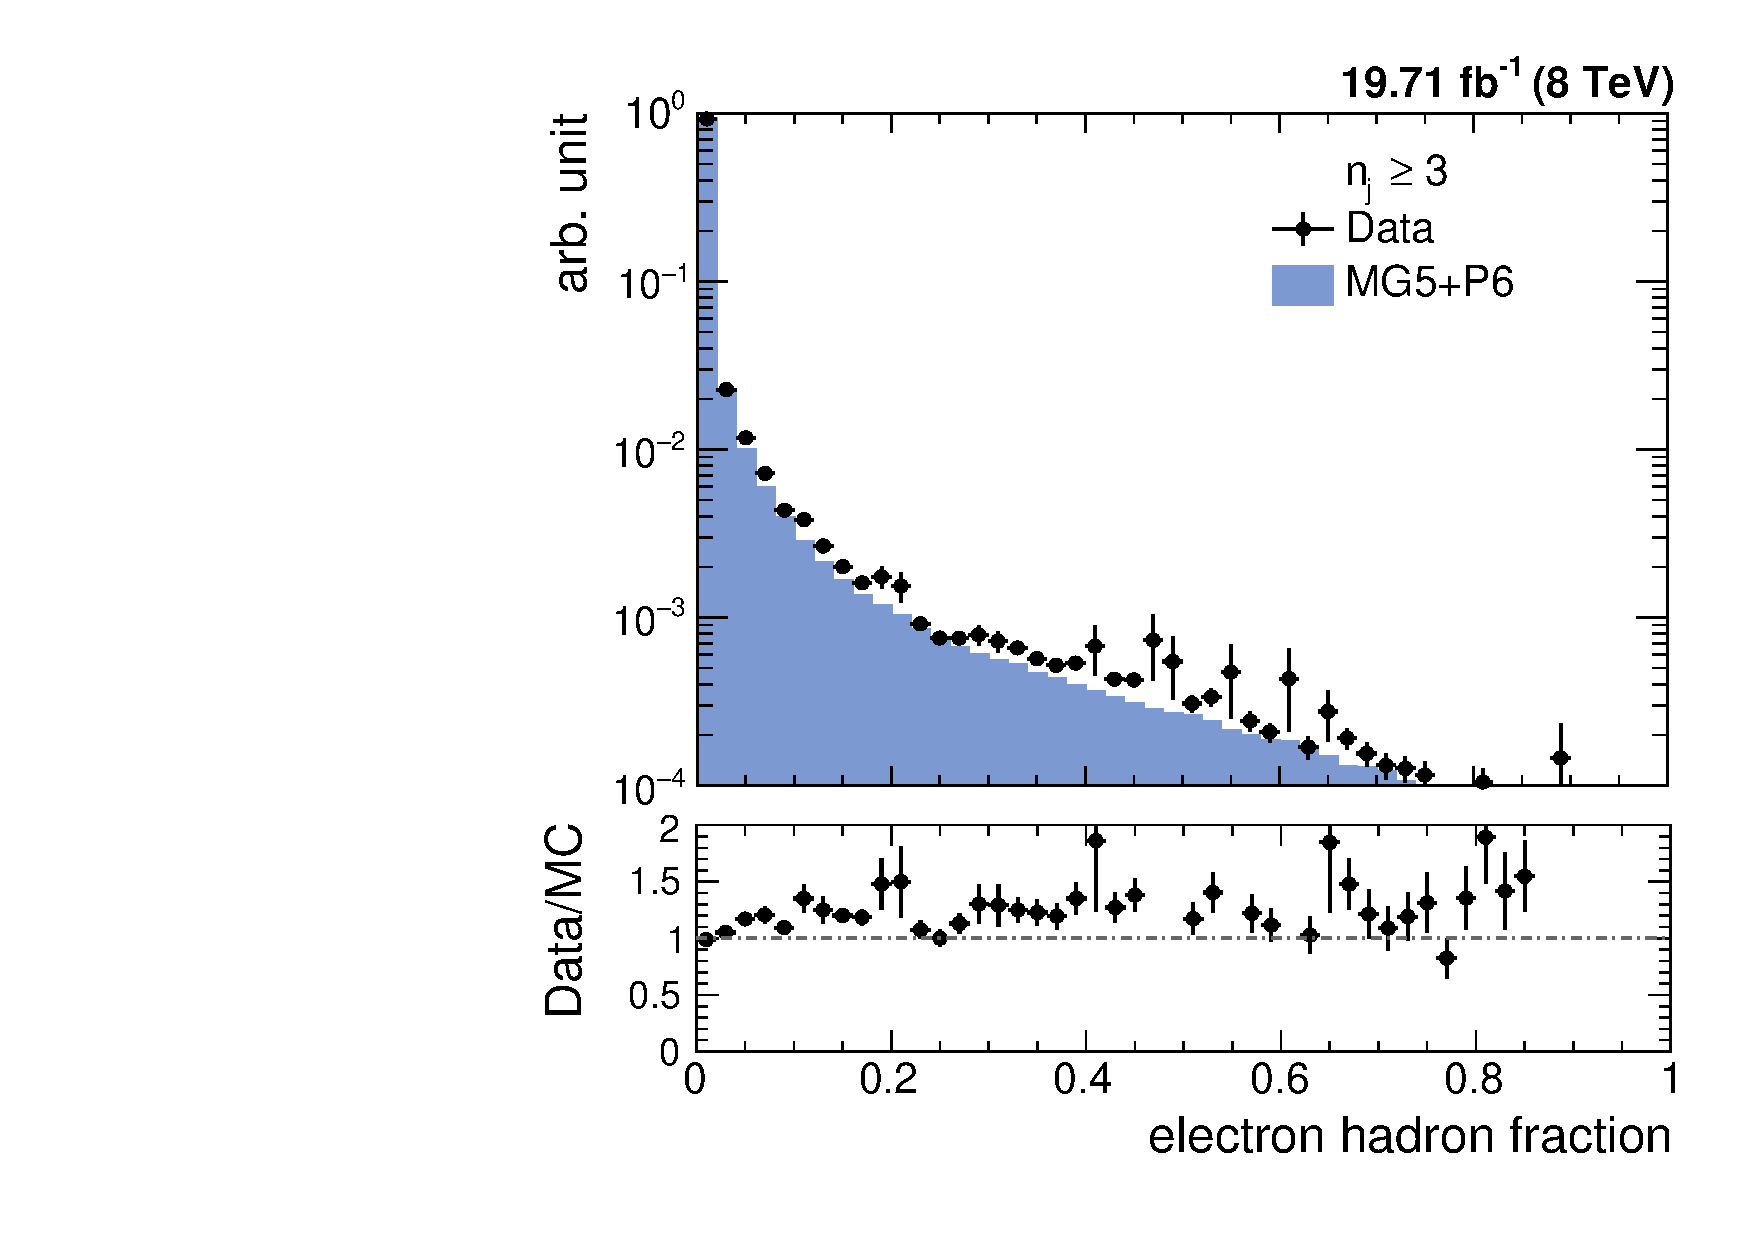
\includegraphics[width=0.5\textwidth]{Plots_HT_2_150/Comparison_ElFrac_3_HT_2_150.pdf}\\
 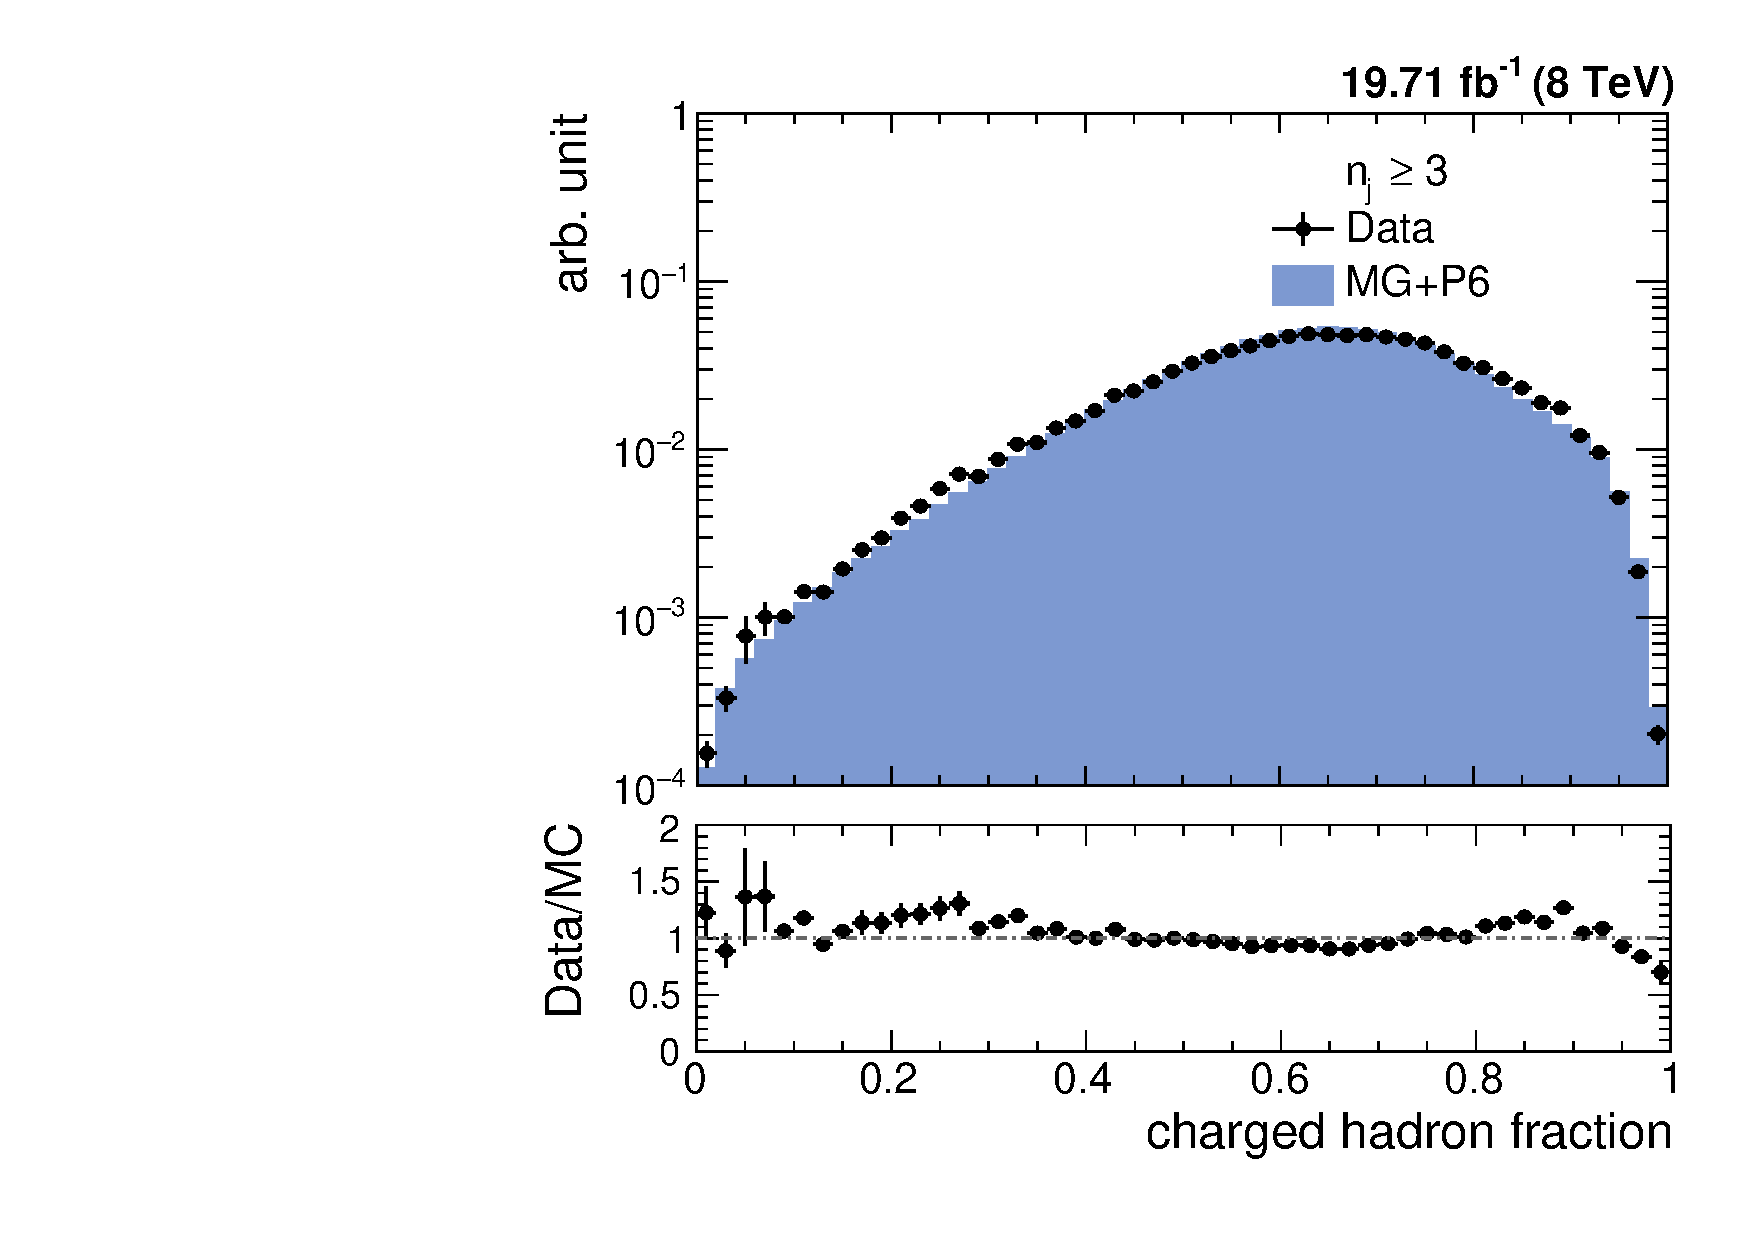
\includegraphics[width=0.5\textwidth]{Plots_HT_2_150/Comparison_ChHadFrac_3_HT_2_150.pdf}%
 \caption{The fractions of jet constituents as observed in data and simulated events for different types of PF candidates for inclusive 3-jet events. Data and simulation are normalized to the same number of events. The distributions are shown after the application of the jet ID.}
 \label{fig:qual3}
 \end{center}
\end{figure} 

\subsubsection{Jet ID Efficiency}
The efficiency of the jet ID as a function of \httwo is studied using a tag-and-probe technique with dijet events. The two leading jets are required to be back-to-back in the azimuthal plane such that $|\Delta\phi - \pi|$ \ls 0.3. One of the dijets is selected randomly as a ``tag'' jet which is required to fulfill the tight jet ID criteria. The other jet is called ``probe'' jet for which it is examined, whether it also passes the tight jet ID. The ID efficiency is defined as the ratio of events where the probe jet passes the ID requirements, over the total number of dijet events. Figure~\ref{fig:ideff} shows the ID efficiency as a function of \httwo for \njt~(left) and \njth~(right) \qm. As expected, the jet ID efficiency is larger than 99\%. The QCD cross section decreases as a function of \httwo and hence the number of events decrease on moving to higher \httwons. Consequently the statistical fluctuations for ID efficiency are larger at higher \httwons.

\begin{figure}[!htbp]
 \begin{center}
 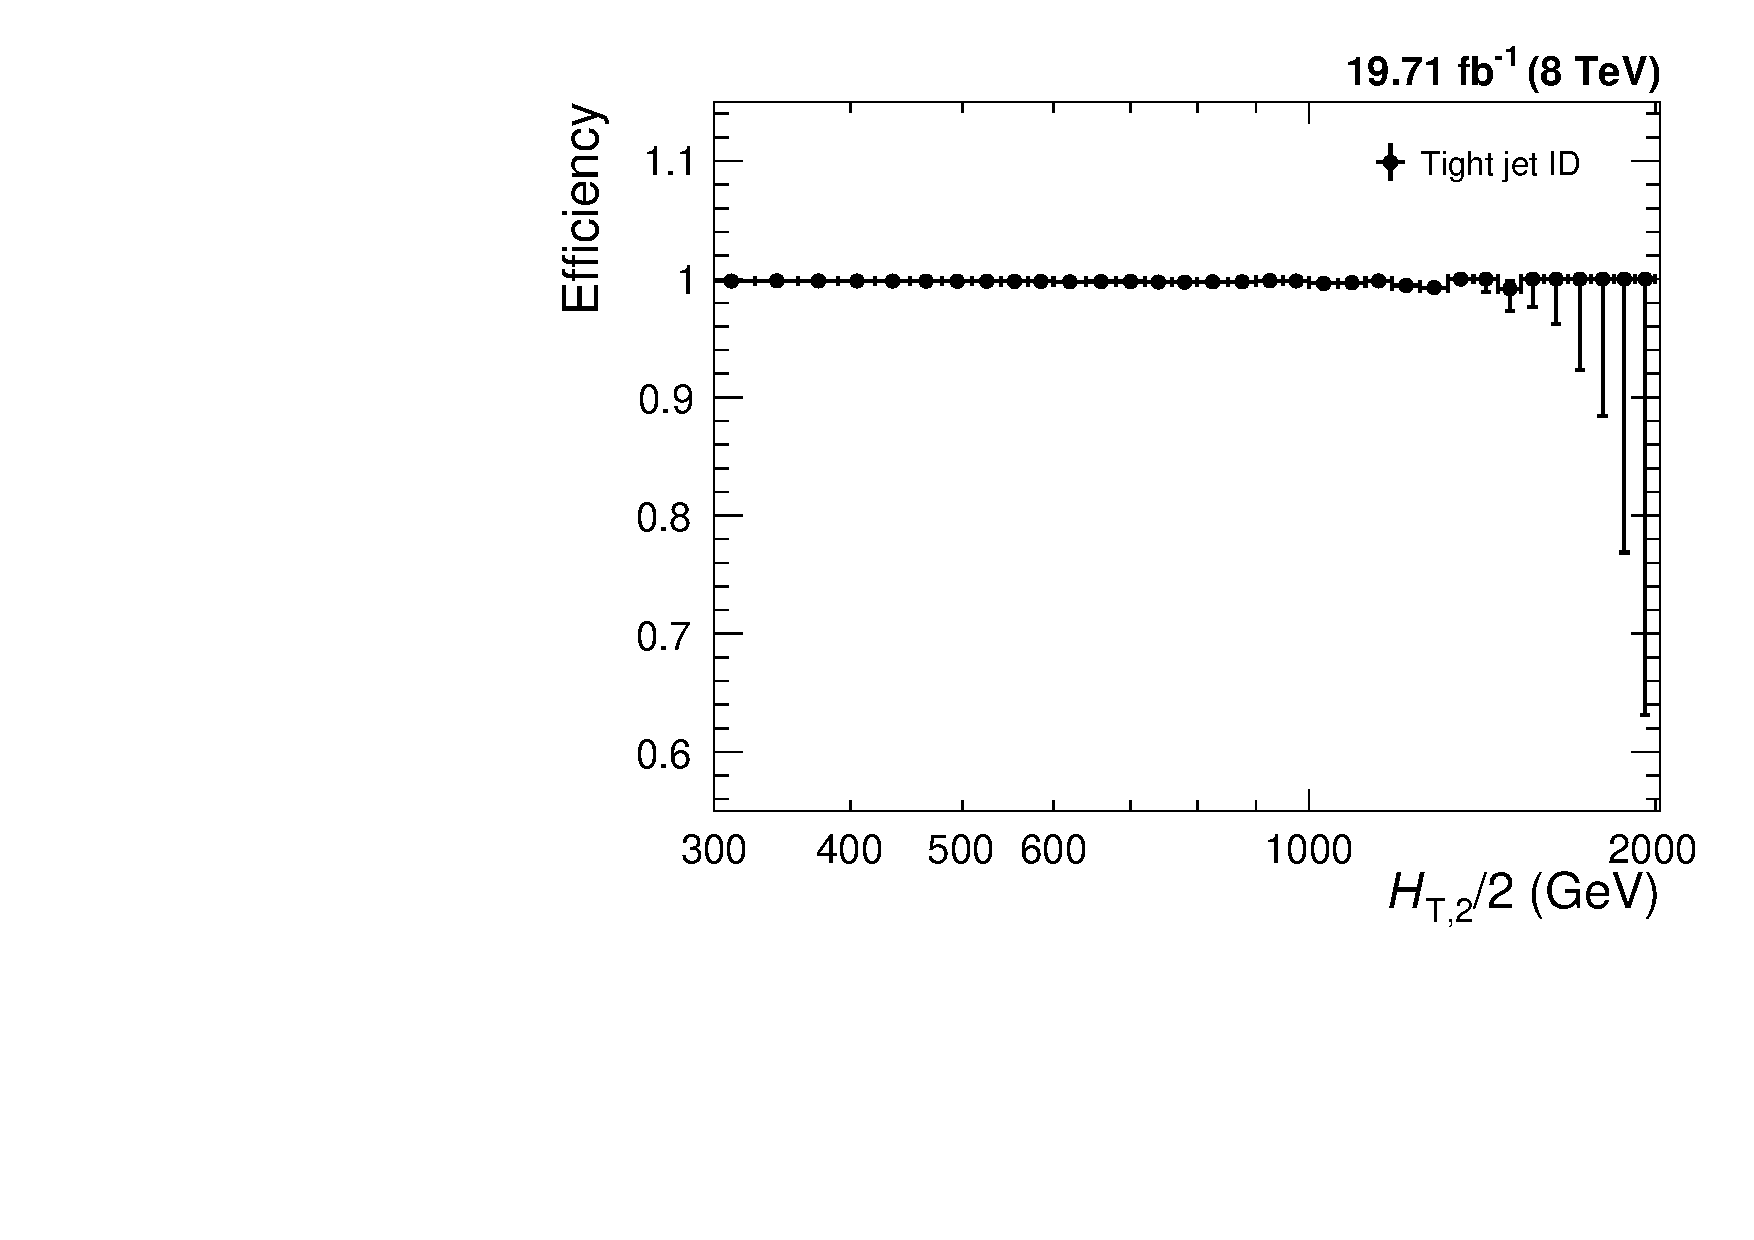
\includegraphics[width=0.5\textwidth]{/home/anter/Desktop/Thesis/Plots_HT_2_150/ID_Efficiency.pdf}%
 ~~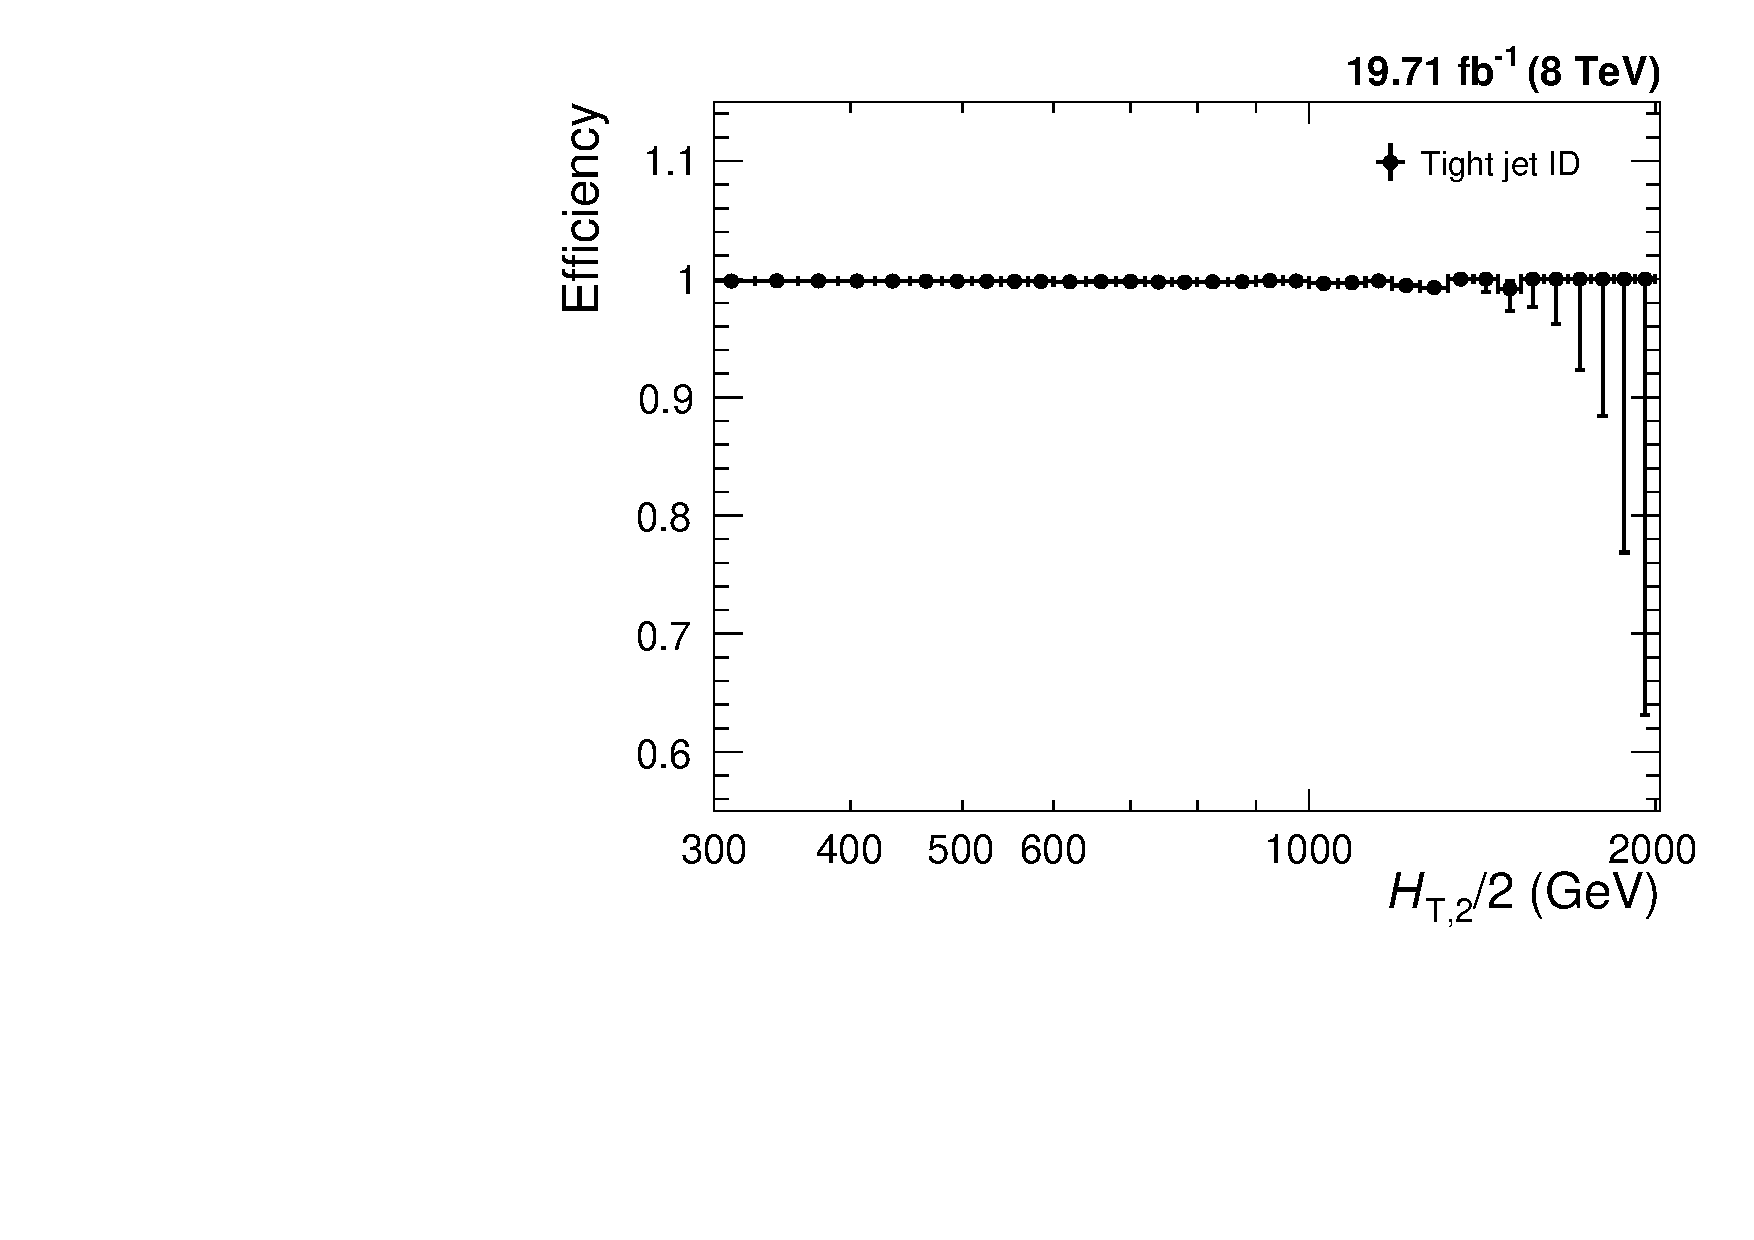
\includegraphics[width=0.5\textwidth]{/home/anter/Desktop/Thesis/Plots_HT_2_150/ID_Efficiency.pdf}%
 \caption{The jet ID efficiency studied using a tag-and-probe technique on dijet event topologies, is shown as a function of \httwo for inclusive 2-jet (left) and 3-jet events (right) and it always exceeds 99\%.}
 \label{fig:ideff}
 \end{center}
\end{figure} 

\subsection{Jet Energy Corrections and Selection}
The measurement presented in this thesis is based on jets clustered from PF candidates using the anti-\kt jet algorithm with a size parameter of 0.7. All the jet energy corrections, described in Sec. \qm~and recommended by CMS, are applied prior to this selection in order to have the correct energy scale of the jets. These comprises different correction levels for jets in data\footnote{The JEC version applied on data is internally referred to as Winter14\_V8} and for jets in simulated events\footnote{The latest JEC for run-independent Monte Carlo Samples are called START53\_V27}. The jet selection, based on phase space cuts on transverse momentum and rapidity of jets in an event, is as follows : 

\begin{itemize}
\item All jets having \pt $>$ 150 \GeV and $|y| < 5.0$ are selected.
\item Events with at least two jets are selected.
\item The two leading jets should have $|y| < 2.5$ and further jets are counted only, if they lie within the same central rapidity range of $|y| < 2.5$. 
\end{itemize}
These cuts assure high detector acceptance and exactly same selection is applied in the measurement, simulated events as well in theoretical calculations for a consistent comparison. 

\section{Comparison with Simulated Events}
\subsection{Pile-up Reweighting}
The official Monte-Carlo samples are generated with distributions for the number of pileup interactions which is meant to roughly cover the conditions expected for each data-taking period. But the number of pile-up events implemented in the simulation $N_{\rm MC} (N_{\rm PU,truth})$, is not exactly the same as the one measured in data $N_{\rm data} (N_{\rm PU,est.})$. To match the pile-up distributions in data and simulated events, the simulated events are reweighted with a weight $w_{\rm PU}$, given by :

\begin{equation}
 {w_{\rm PU} = \frac {N_{\rm data} (N_{\rm PU,est.})/\sum N_{\rm data}} {N_{\rm MC} (N_{\rm PU,truth)}/\sum N_{\rm MC}}}
\end{equation}
Figure~\ref{fig:pileup} shows the number of reconstructed vertices before and after reweighting. The significant mismatch of the pile-up distributions in data and simulated events, which is present before the reweighting, completely vanishes. 

\begin{figure}[!htbp]
 \begin{center}
 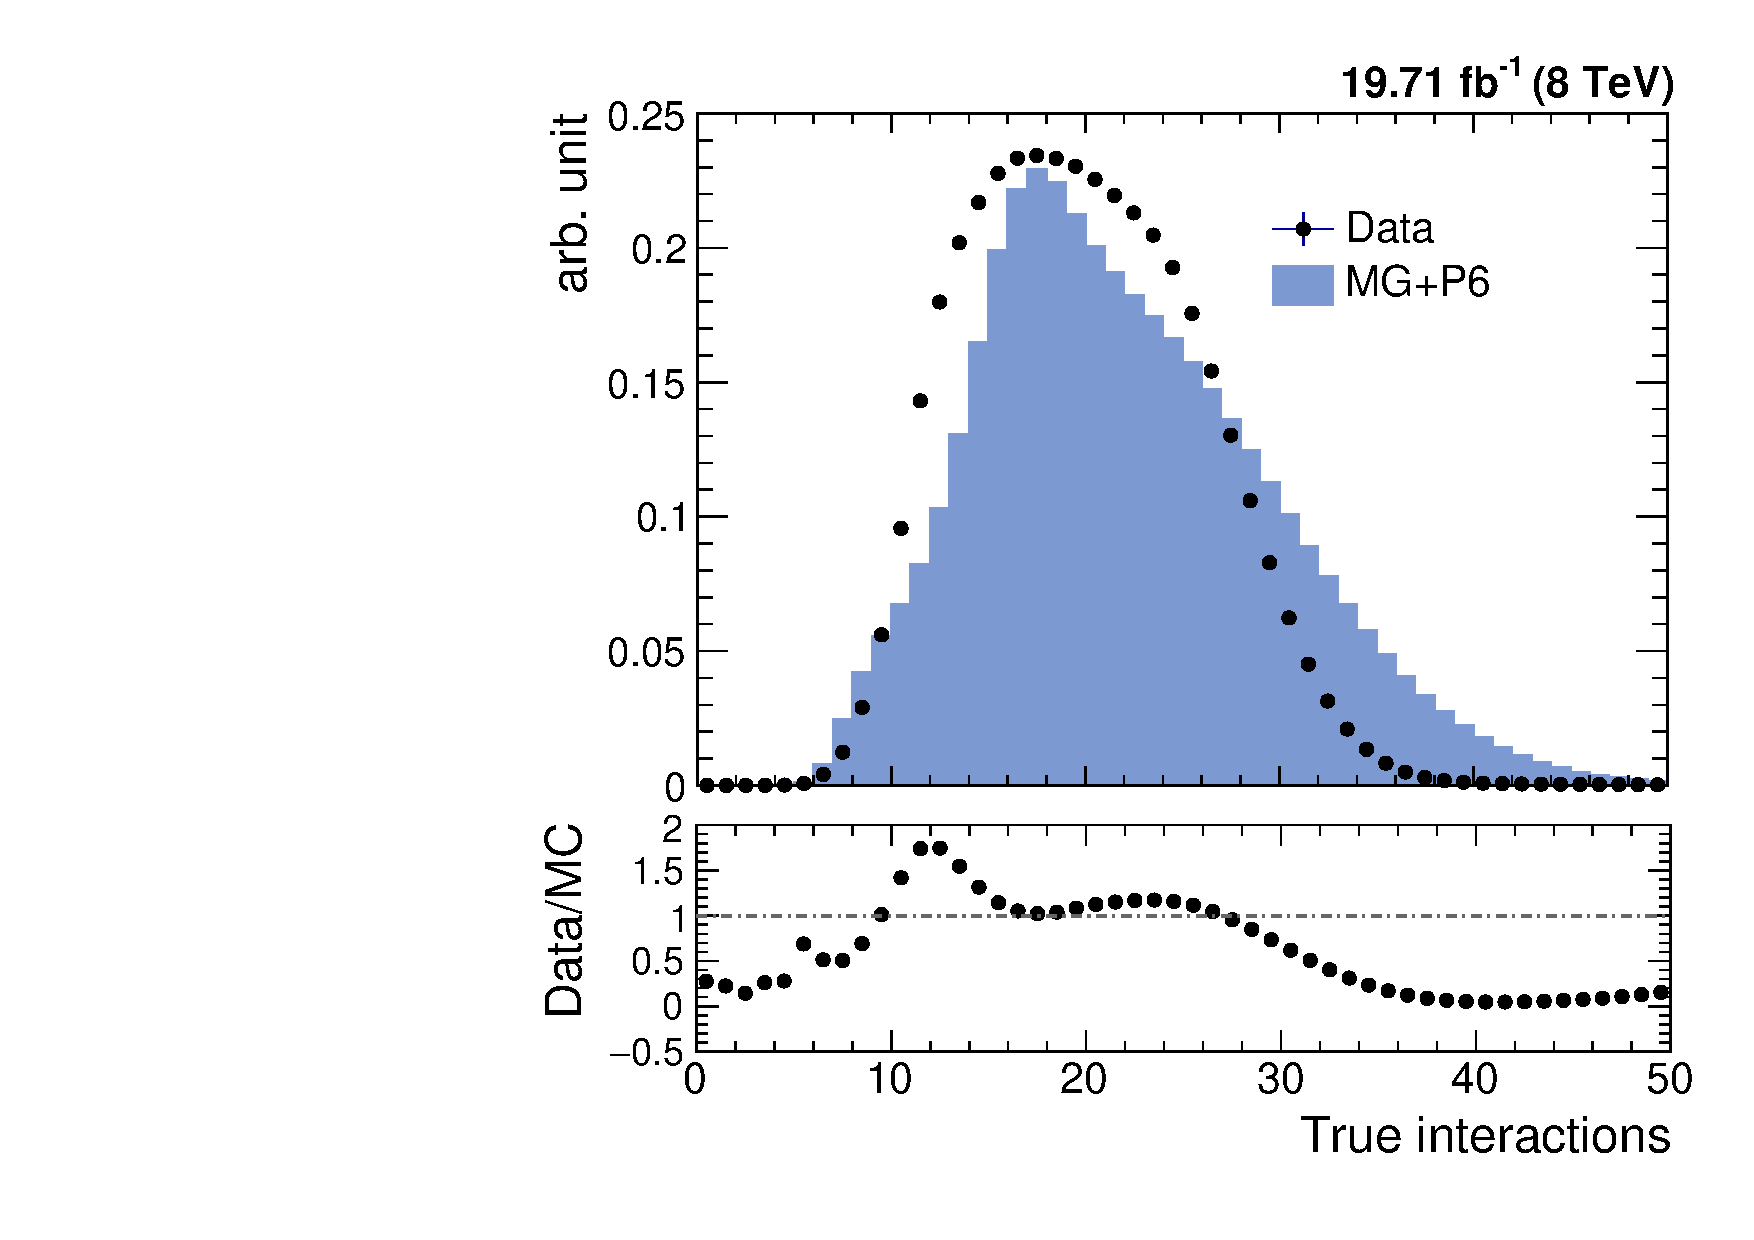
\includegraphics[width=0.51\textwidth]{Plots_HT_2_150/Nvertices.pdf}%
 ~~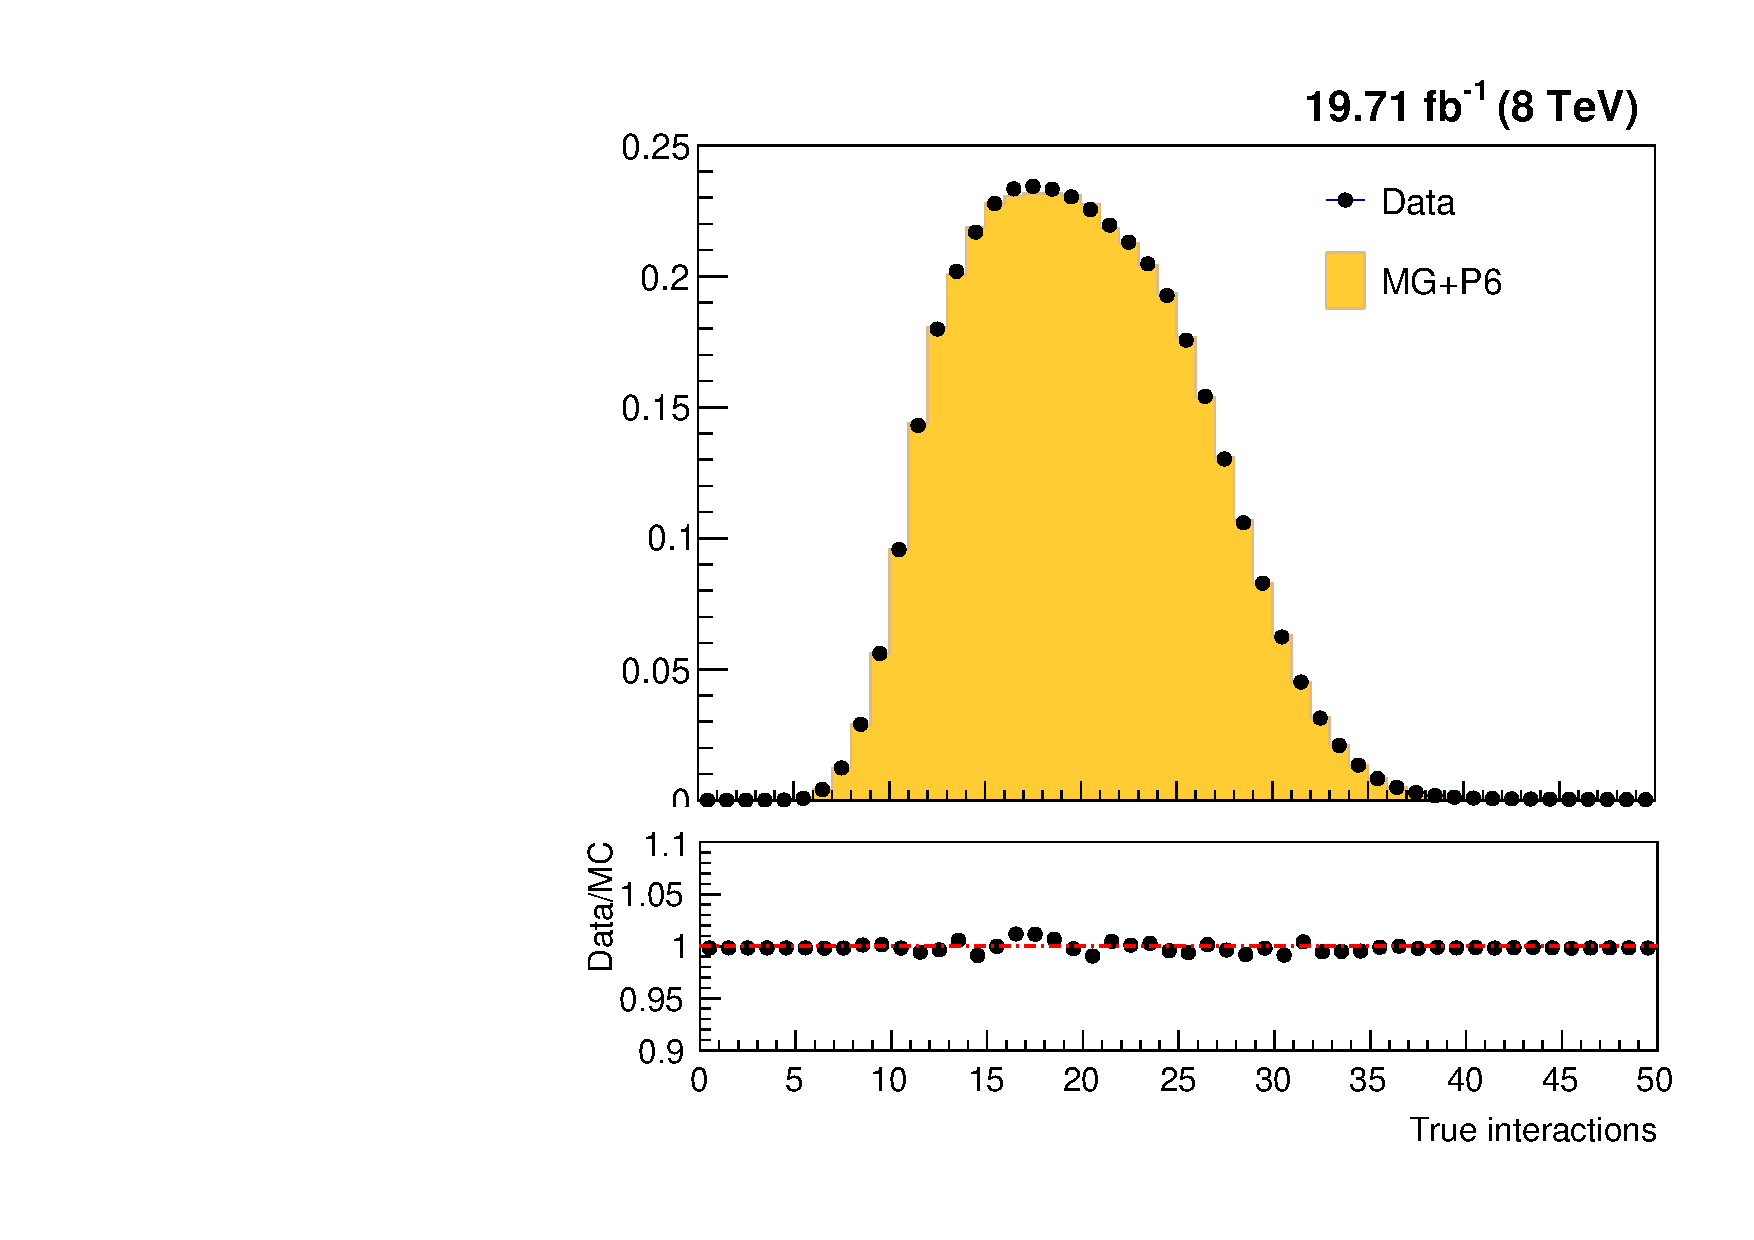
\includegraphics[width=0.51\textwidth]{Plots_HT_2_150/Nvertices_weight.pdf}
 \caption{Number of reconstructed vertices in data and simulated events before (left) and after (right) the pile-up reweighting.}
 \label{fig:pileup}
 \end{center}
\end{figure}

\subsection{Cross Section Comparison}
The measured data distribution of differential cross section at detector level is compared to the predictions of Monte Carlo simulation using \MadGraphF generator interfaced with \PYTHIAS (\MGP) and including the detector simulation as well as to a fixed-order prediction of \NLOJETPP. Figure~\ref{fig:comp_all} shows the comparison of differential cross section as a function of \httwo for \njt~(left) and \njth~(right), for data (black solid circles), \MGP~MC (red empty circles) and NLO (histogram). The bottom panel in each plot shows the ratio of data to the MC predictions (red line) as well as to the NLO predictions (blue line). The NLO predictions on parton level are not corrected for non-perturbative effects. Still the NLO predictions describe the data better as compared to the LO MC simulations. The sufficient data for \njt~and \njth~events are available up to $\httwo = 2\TeV$ and $1.68\TeV$, respectively. As mentioned in Sec.~\ref{} \qm that the minimum kinematical cut on \httwo is 300 GeV. Hence the observable is studied in the range 300 GeV $\leq$ \httwo $<$ 2 TeV for \njt~ and   
300 GeV $\leq$ \httwo $<$ 1.68 TeV for \njth~events.

\begin{figure}[!htbp]
 \begin{center}
 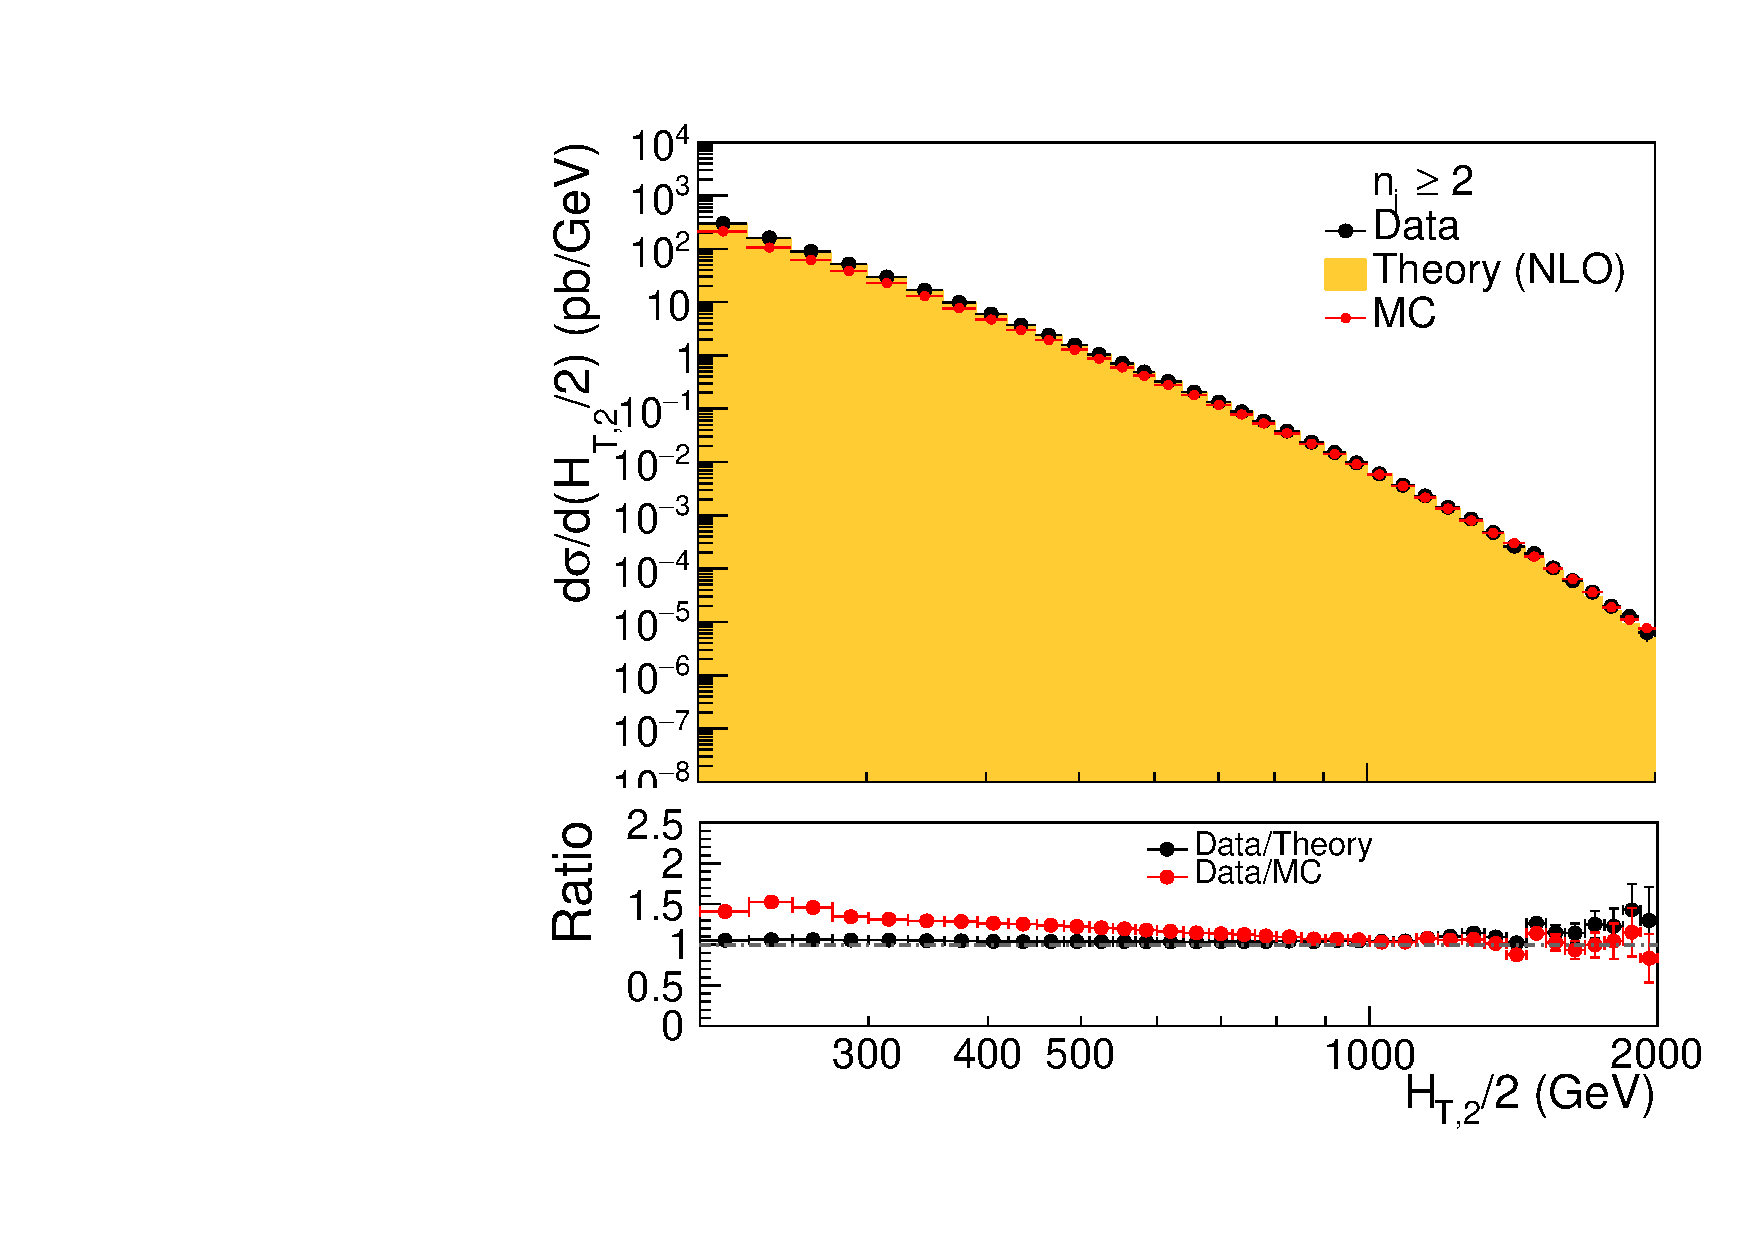
\includegraphics[width=0.51\textwidth]{Plots_HT_2_150/Comparison_all_2_HT_2_150.pdf}%
 ~~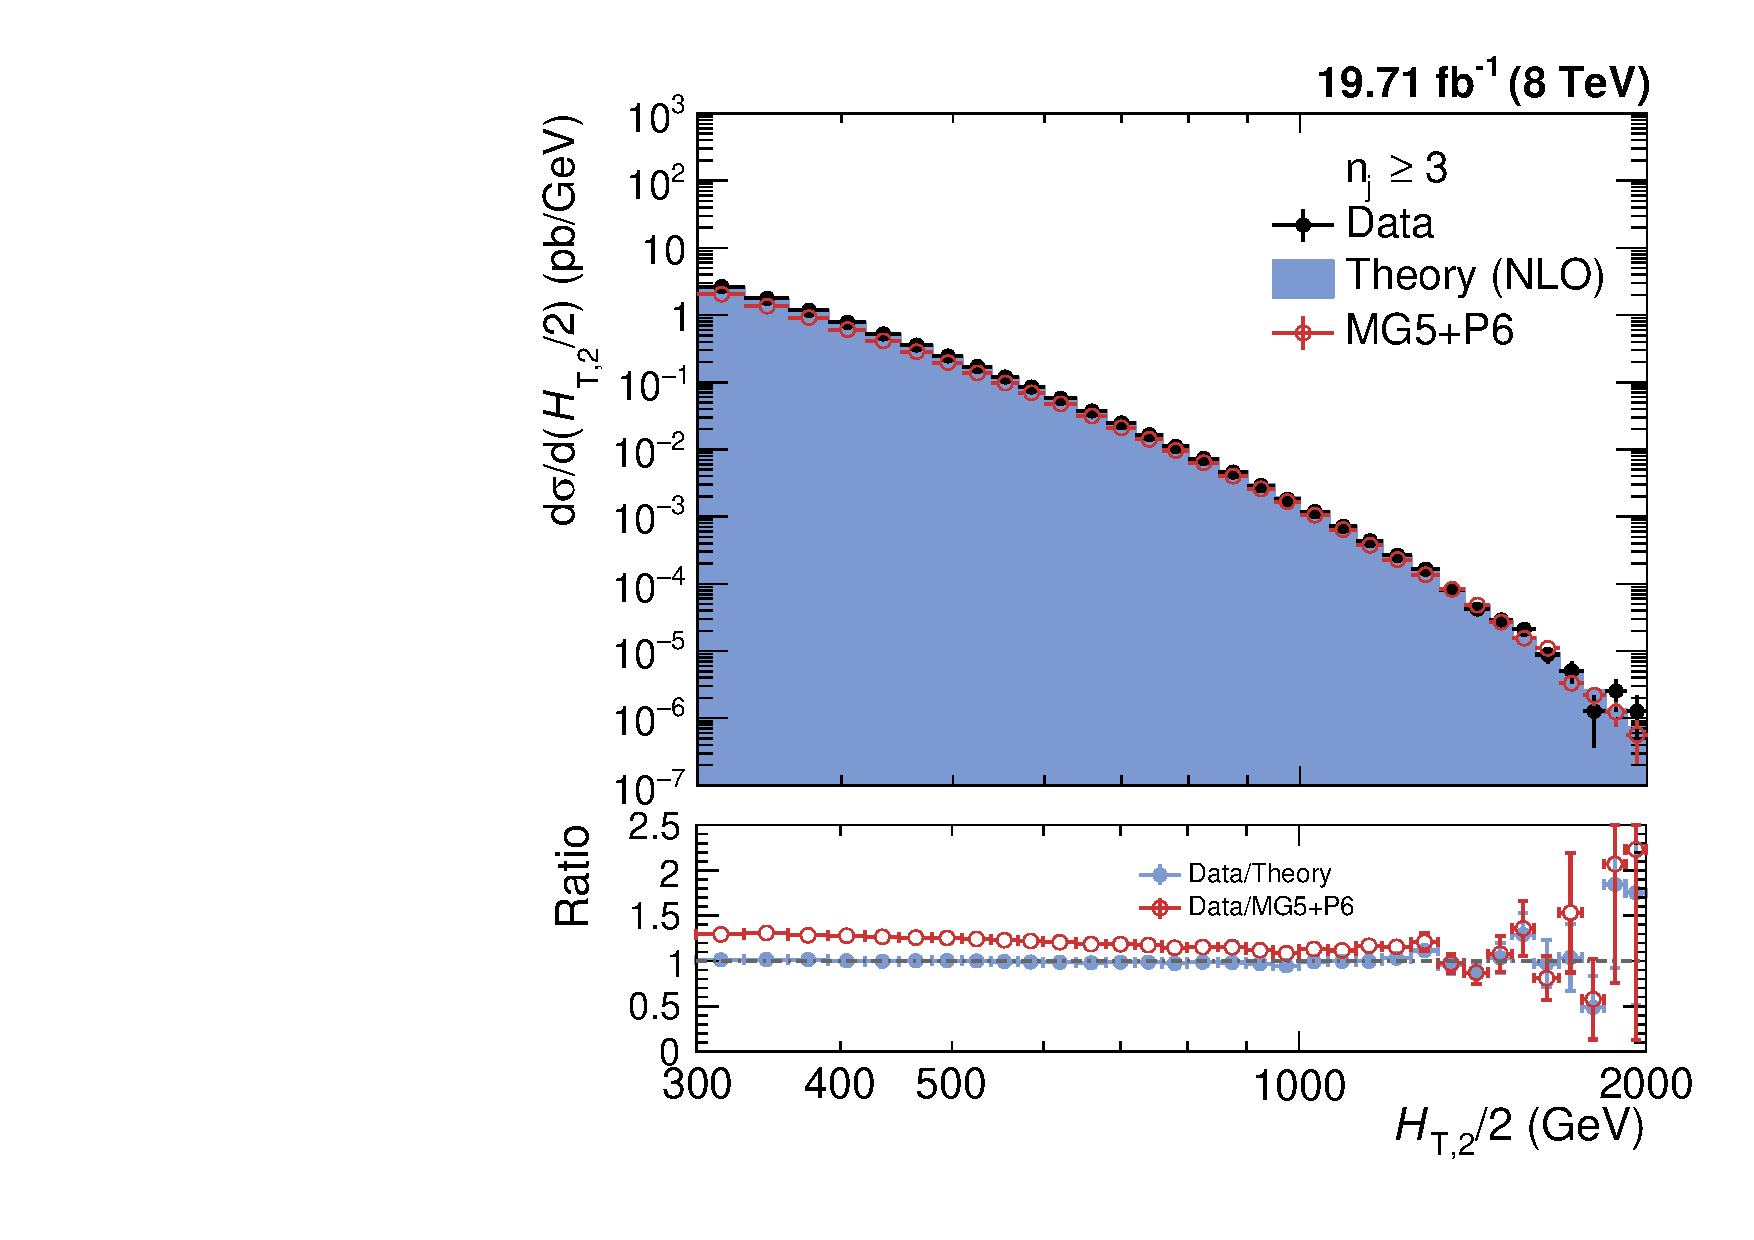
\includegraphics[width=0.51\textwidth]{Plots_HT_2_150/Comparison_all_3_HT_2_150.pdf}\\
 \caption{The differential cross sections are compared for data (black solid circles) and LO \MadGraphF \plus \PYTHIAS (\MGP) Monte Carlo (red empty circles), at reconstructed level with NLO theory predictions (histogram), as a function \httwo for inclusive 2-jet events (left)and 3-jet events (right). Ratios of data to the Monte Carlo predictions (red line) as well as to the NLO predictions (blue line) are shown in bottom panel of each plot.}
 \label{fig:comp_all}
 \end{center}
\end{figure}

\section{Jet Energy Resolution (JER)}
\label{sec:Resolution}
In an ideal experiment, the value of a physical quantity would be determined exactly with an infinite precision. For e.g. whenever a particle with energy E passes an ideal calorimeter having infinite resolution, the measured energy should always be equal to E. But in real detector, the measured energy of the above mentioned particle might differ from the value E. This shift of the measured quantity from its true value may be due to detector noise, uncertainties in the calibration, non-linearity of the response etc. Hence this results in the finite value of the detector resolution (JER). In such case, the measured values of energy of different particles, crossing the same detector with same energy E, will be different. The set of measurements of this type would in the form of a gaussian distribution, centered around the true value of the measured quantity, whose width is generally interpreted as detector resolution. The resolution of a detector indicates that how precise it is able to measure a given physical observable. The narrower the distribution, the higher the resolution is and hence the more precise is the detector. The importance of the measurement of the detector resolution lies in the fact that it indicates how much the measured value of the observable differs from the true one. %The measurement of detector resolution helps in the determination of the histogram binning of the observable to be studied. In binned histograms, it is possible that the measured quantity may migrate from one bin to another with respect to their true value. To avoid these migrations, the bin width should be at least two-three times larger than the detector resolution in that particular bin. The bin widths may also differ between each other for the same observable.

Due to finite resolution of the CMS detector, the measured transverse momentum of jets gets smeared. Since the observable in this study i.e. \httwo is the average sum of transverse momentum of leading and sub-leading jets, the resolution of the detector has to be studied in terms of the observable. CMS detector simulation based on \MGP~MC event generators is used to determine the resolution as both the particle and reconstructed level information is available. The jets clustered from stable generator particles called Gen jets as well as from particle flow candidates reconstructed from the simulated detector output called Reco jets, are used. The studies of the \JetMet working group at CMS has shown that the jet energy resolution in data is actually worse than in simulation \cite{JER}. So the reconstructed jet transverse momentum needs to be smeared additionally to match the resolution in data. Table~\ref{tab:resolution} shows the scaling factors (c) which need to be applied on the transverse momentum of simulated reconstructed jets. The scaling factors depend on the absolute $\eta$ of the jet. The uncertainty on these measured scaling factors needs to be taken into account in a physics analysis. This is done by smearing the reconstructed jets with two additional sets of scaling factors, c$_{up}$ and c$_{down}$, that correspond to varying the factors up and down respectively, by one sigma and evaluating the impact of these new sets. 

\begin{table}[!htbp]
\centering
 \caption{\JetMet working group at CMS has shown that the jet energy resolution in data is actually worse than in simulation \cite{JER}. The scaling factors need to be applied to the reconstructed jet transverse momentum in simulated events to match the resolution in data. The uncertainty on the resolution is given by an upwards and downwards variation c$_{up}$ and c$_{down}$ of the smearing factor c$_{central}$.}
 \label{tab:resolution}
 \vspace{2mm}
 \begin{tabular}{cccccc}
  \hline\hline
    $\eta$  & $0.0$ -- $0.5$ & $0.5$ -- $1.1$ & $1.1$ -- $1.7$ & $1.7$ -- $2.3$ & $2.3$ -- $2.8$  \rbthm\\ \hline

    c$_{central}$    & 1.079   & 1.099   & 1.121    & 1.208   & 1.254    \rbtrr\\
    c$_{down}$       & 1.053   & 1.071   & 1.092    & 1.162   & 1.192    \rbtrr\\
    c$_{up}$         & 1.105   & 1.127   & 1.150    & 1.254   & 1.316    \rbtrr\\ 
    \hline\hline
  \end{tabular}
\end{table}

The reconstructed jet \pt is smeared randomly using a gaussian width widened by the scaling factor (c$_{central}$) 
\begin{equation}
\pt \rightarrow Gauss\bigg(\mu = \pt, \sigma = \sqrt{c^2_{central} - 1} \cdot {\rm JER}(\pt)\bigg)
\end{equation}

where JER(\pt) is the resolution determined as a function of jet \pt using \MGP~MC simulated events. After smearing transverse momentum of each reco jet, \httwo is calculated from both generator particle jets (Gen \httwons) as well as the particle flow or reconstructed jets (Reco \httwons). Then the response is calculated as defined in the Eq.~\ref{eq:res}. 
\begin{equation}
\label{eq:res}
  R = \frac{{\rm Reco}~\httwo}{{\rm Gen}~\httwo}
\end{equation}

\begin{figure}[h]
  \begin{center}
    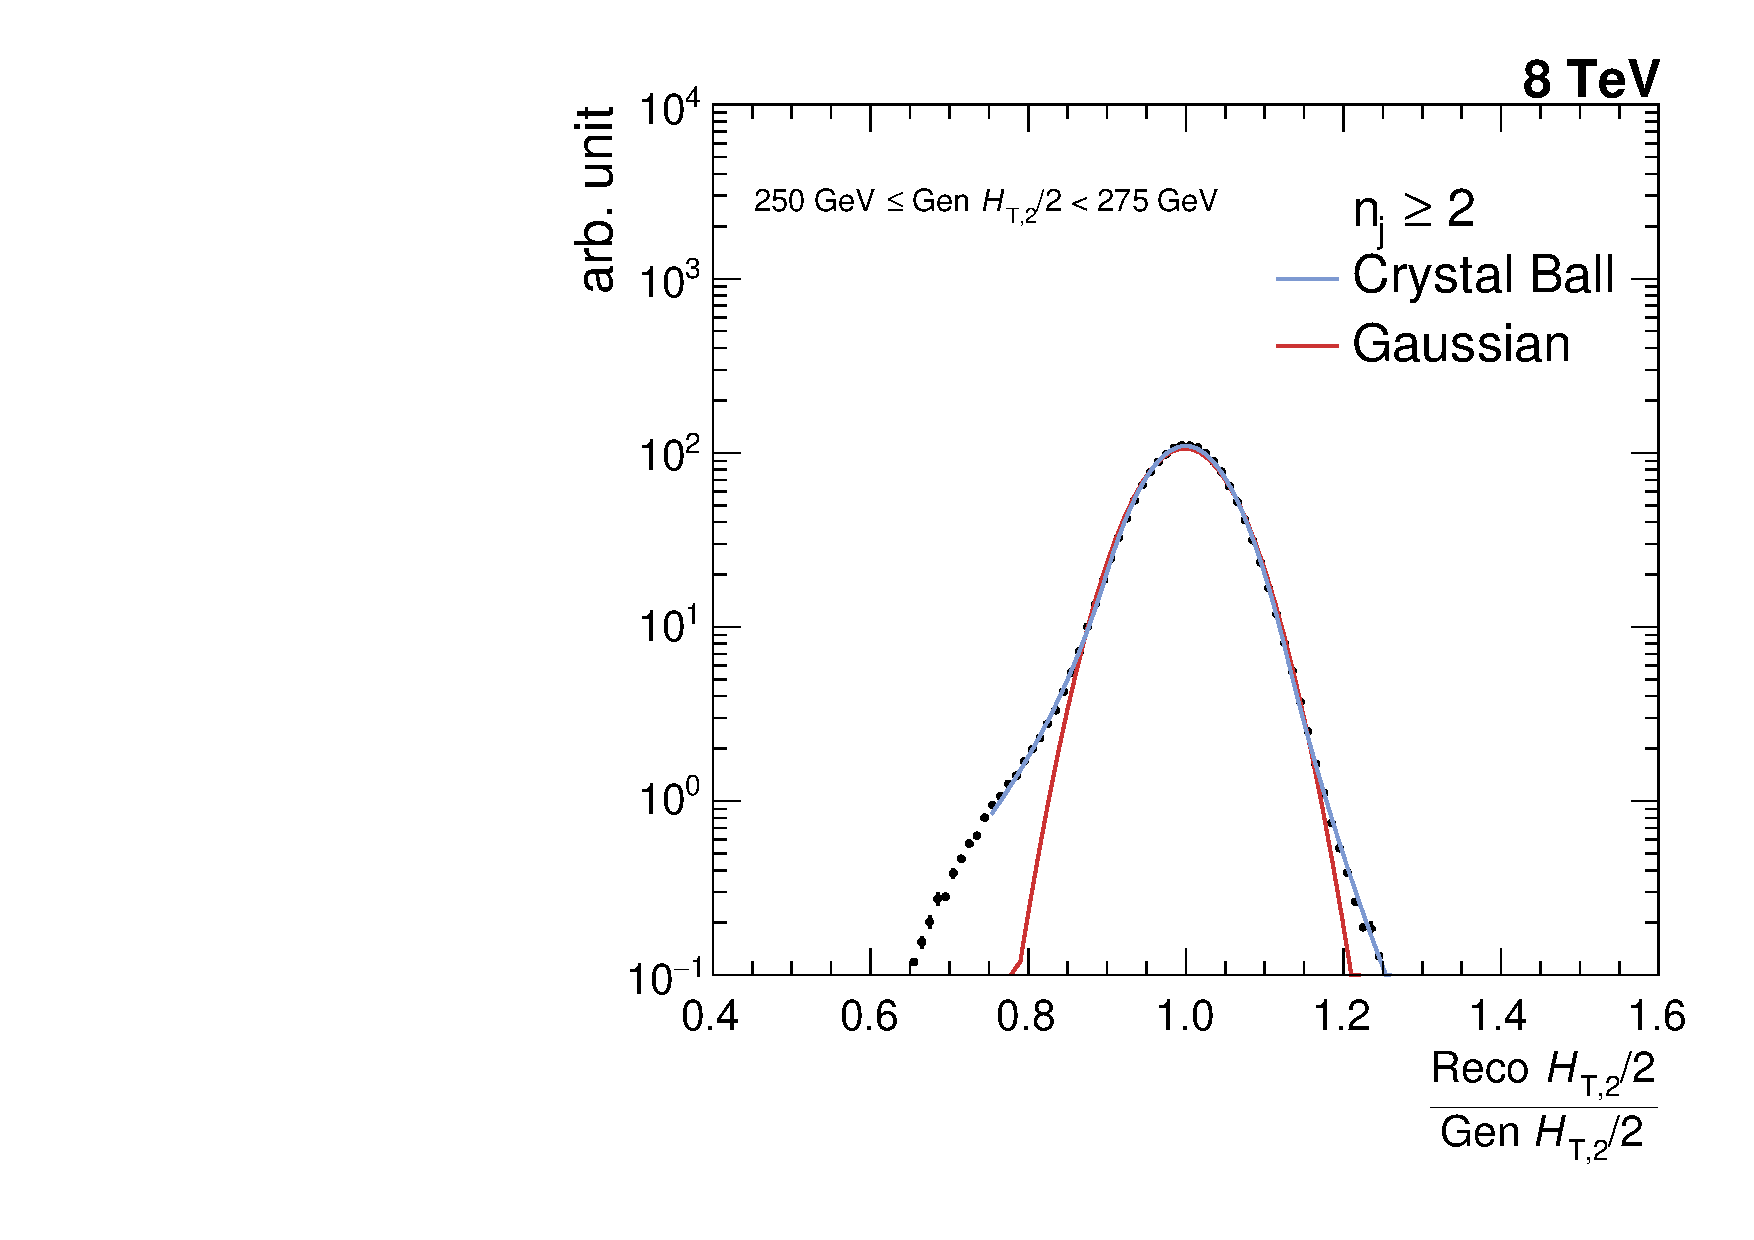
\includegraphics[width=0.51\textwidth]{Plots_HT_2_150/Fit_Res_2_final_crystal_genbin_250-275_crystal_nomet.pdf}%
    ~~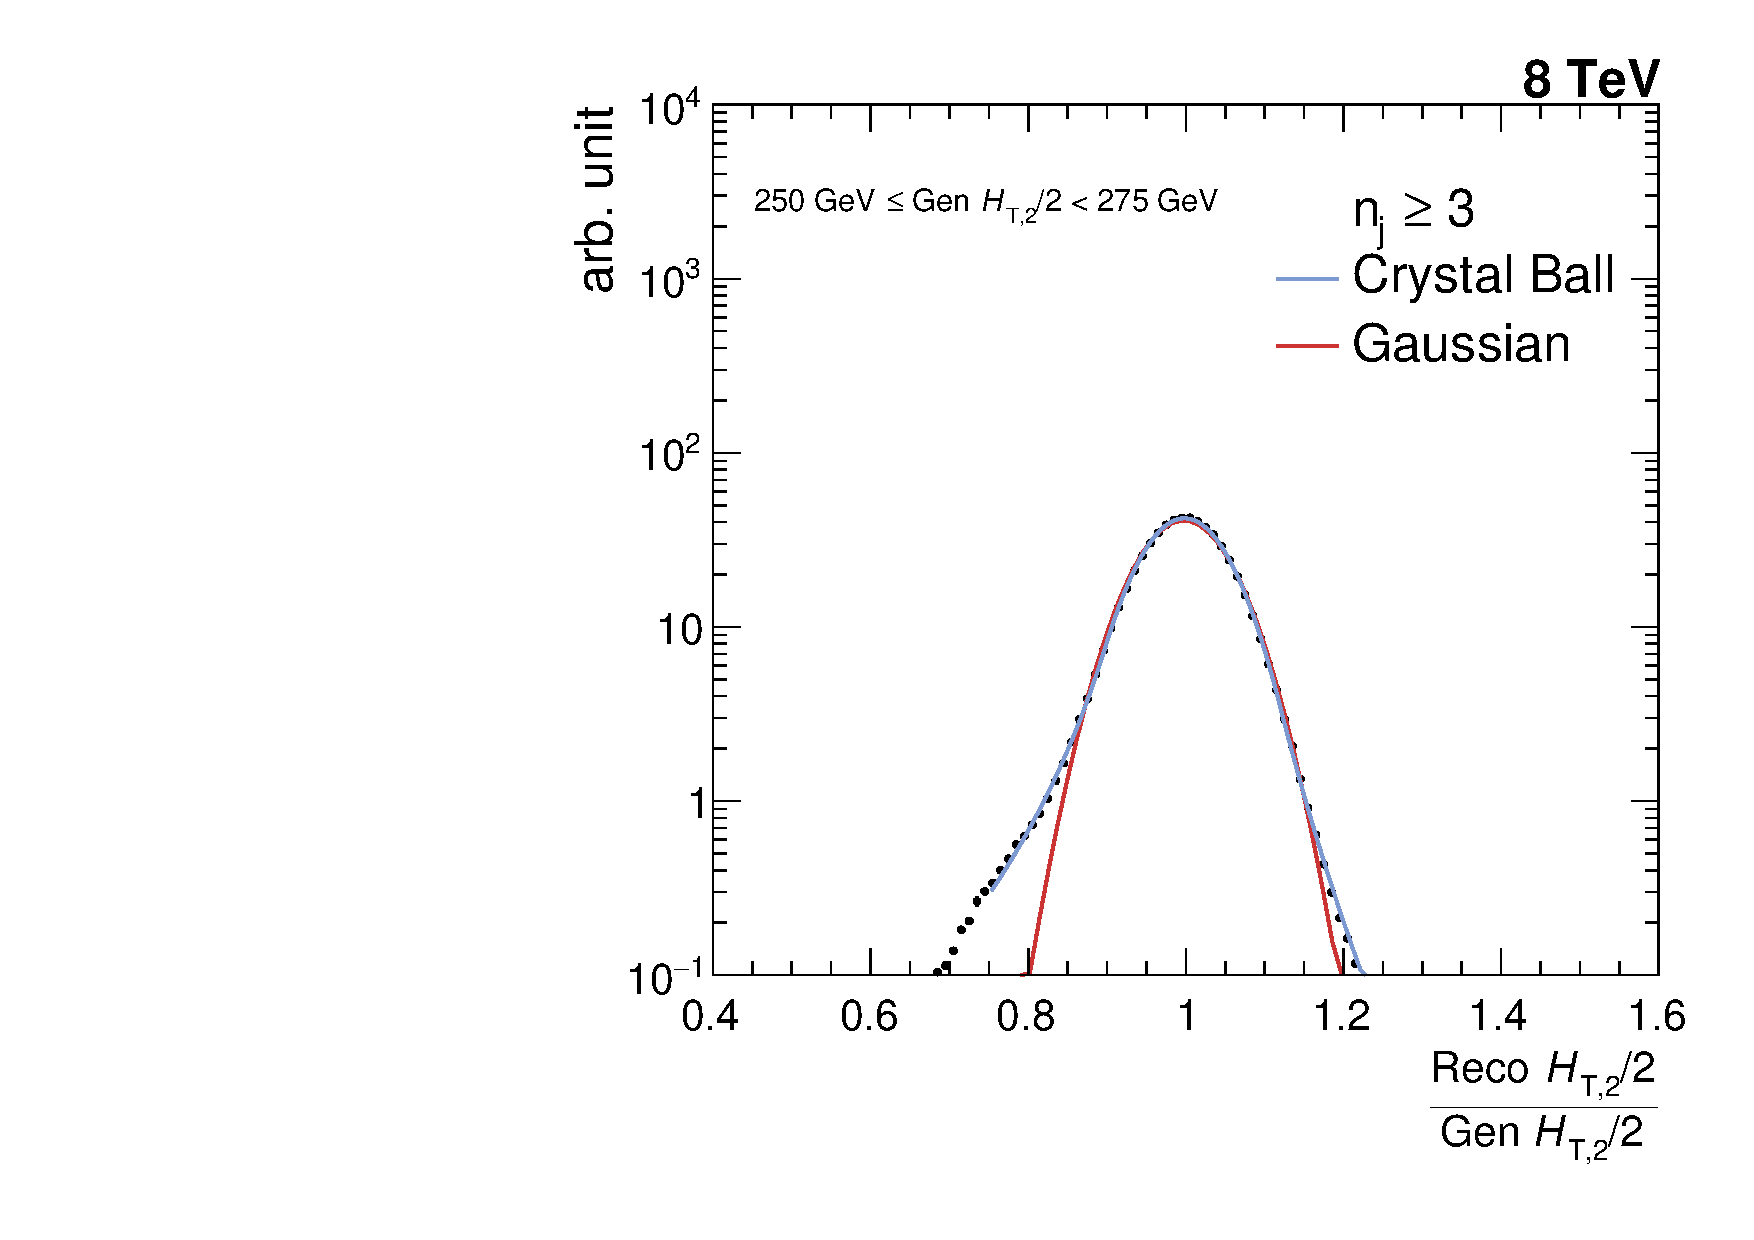
\includegraphics[width=0.51\textwidth]{Plots_HT_2_150/Fit_Res_3_final_crystal_genbin_250-275_crystal_nomet.pdf}
    \caption{Fitting of the resolution distribution as a function of \httwo for inclusive 2-jet (left) and for inclusive 3-jet events (right). The blue line shows the double-sided Crystal Ball function fit of $\frac{{\rm Reco}~\httwo}{{\rm Gen}~\httwo}$ in each Gen \httwo bin, overlayed by Gaussian fitting the core of the resolution (red line).}
    \label{fig:fit_gauss}
  \end{center}
\end{figure}

The width of the response distribution in a given Gen \httwo bin is interpreted as the resolution which can in good approximation be described by the $\sigma$ of a Gaussian fit to the core of distribution. To take into account the non-Gaussian tails of the jet response distribution, a double-sided Crystal-Ball function is used. The resolution as a function of \httwo is calculated separately for both \njt~and \njth~events. A fit example for one Gen \httwo bin is shown in Fig.~\ref{fig:fit_gauss} for \njt~(left) and inclusive 3-jet events (right). Here the black dots represent the jet response distribution and the double-sided Crystal-Ball fit (blue line) is overlayed by the Gaussian fit (red line). The resolution in each Gen \httwo bin is then plotted as a function of Gen \httwo. As expected, it has been observed from Fig.~\ref{fig:res_comp} that the Crystal Ball function better describes the measured distributions, especially in the low-\httwo region where the non-Gaussian tails are more pronounced. Hence the Crystal Ball function is preferred to determine the resolution.

\begin{figure}[h]
 \begin{center}
 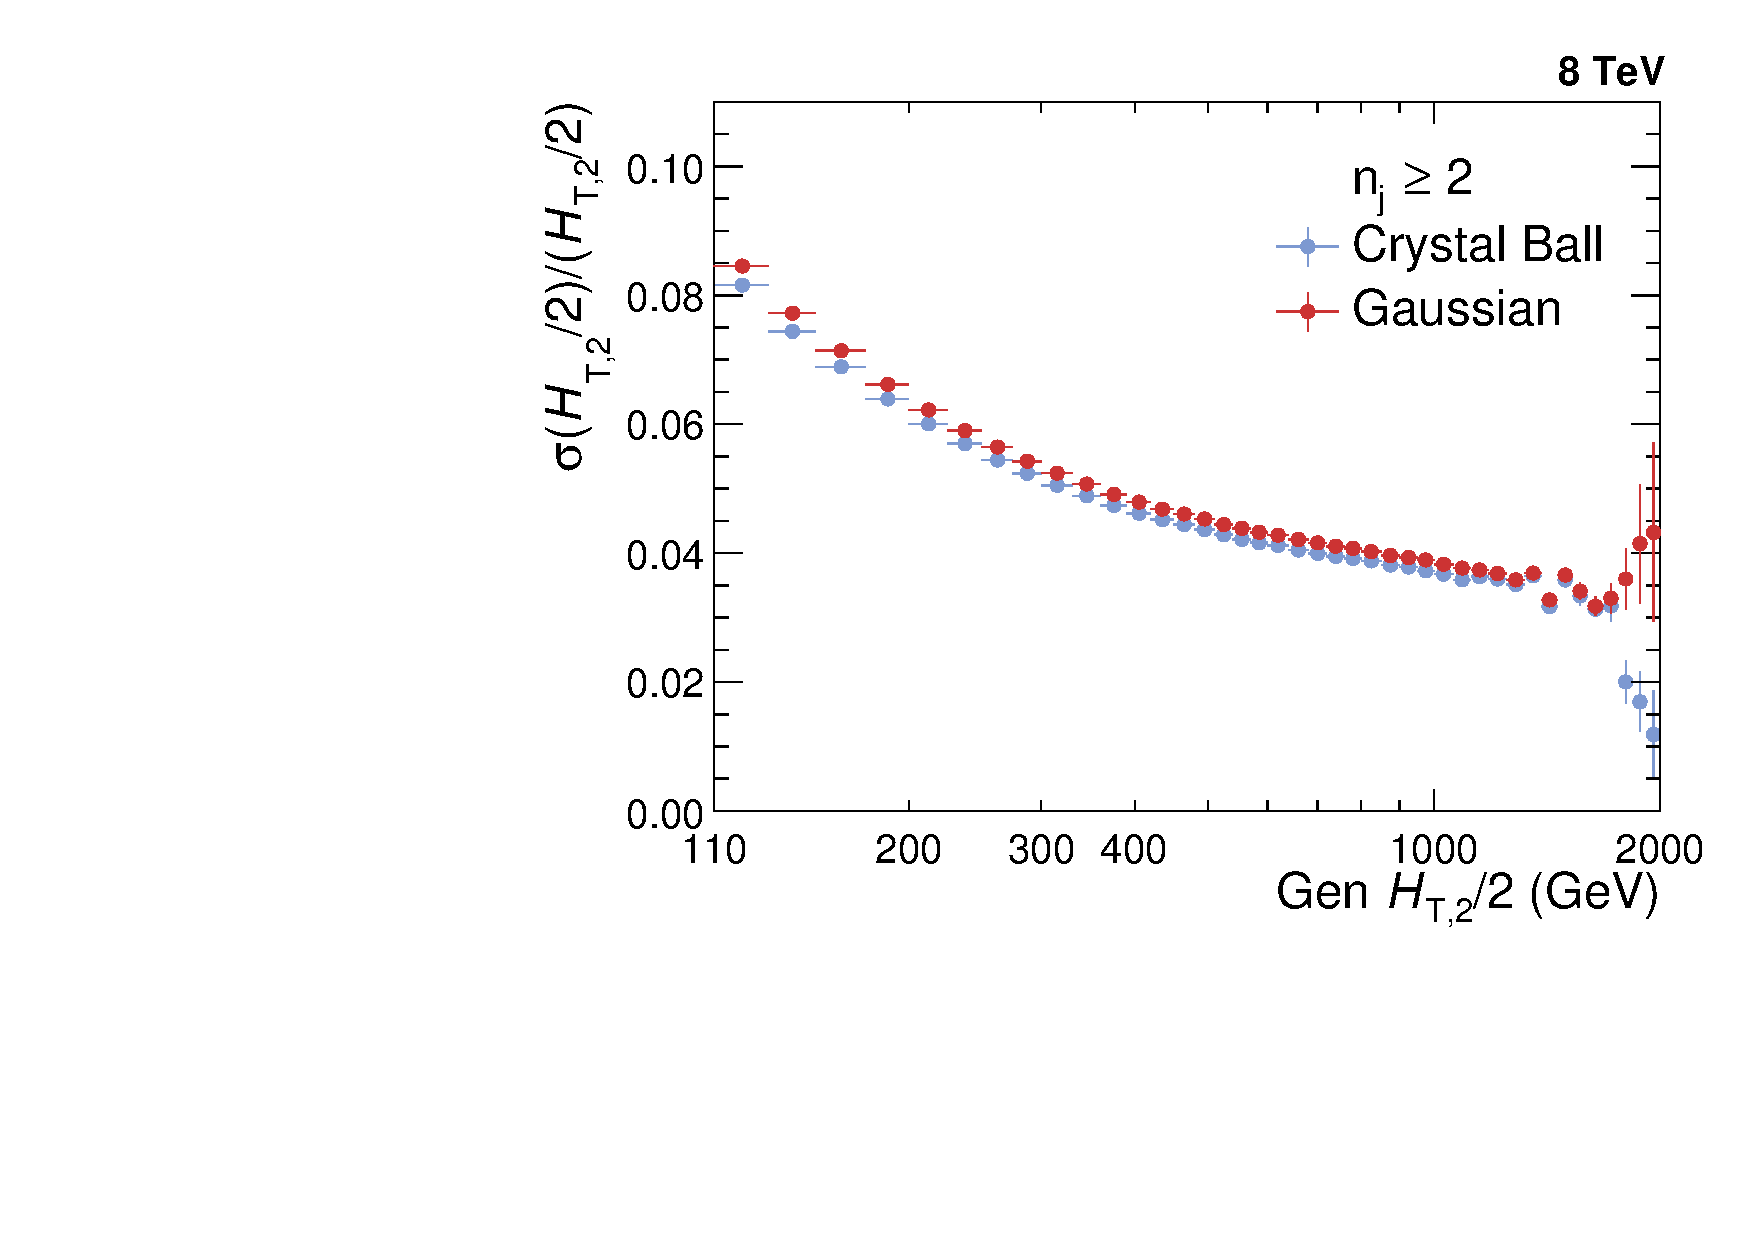
\includegraphics[width=0.51\textwidth]{Plots_HT_2_150/Comparison_Resolution_Crystal_Gauss_2.pdf}%
 ~~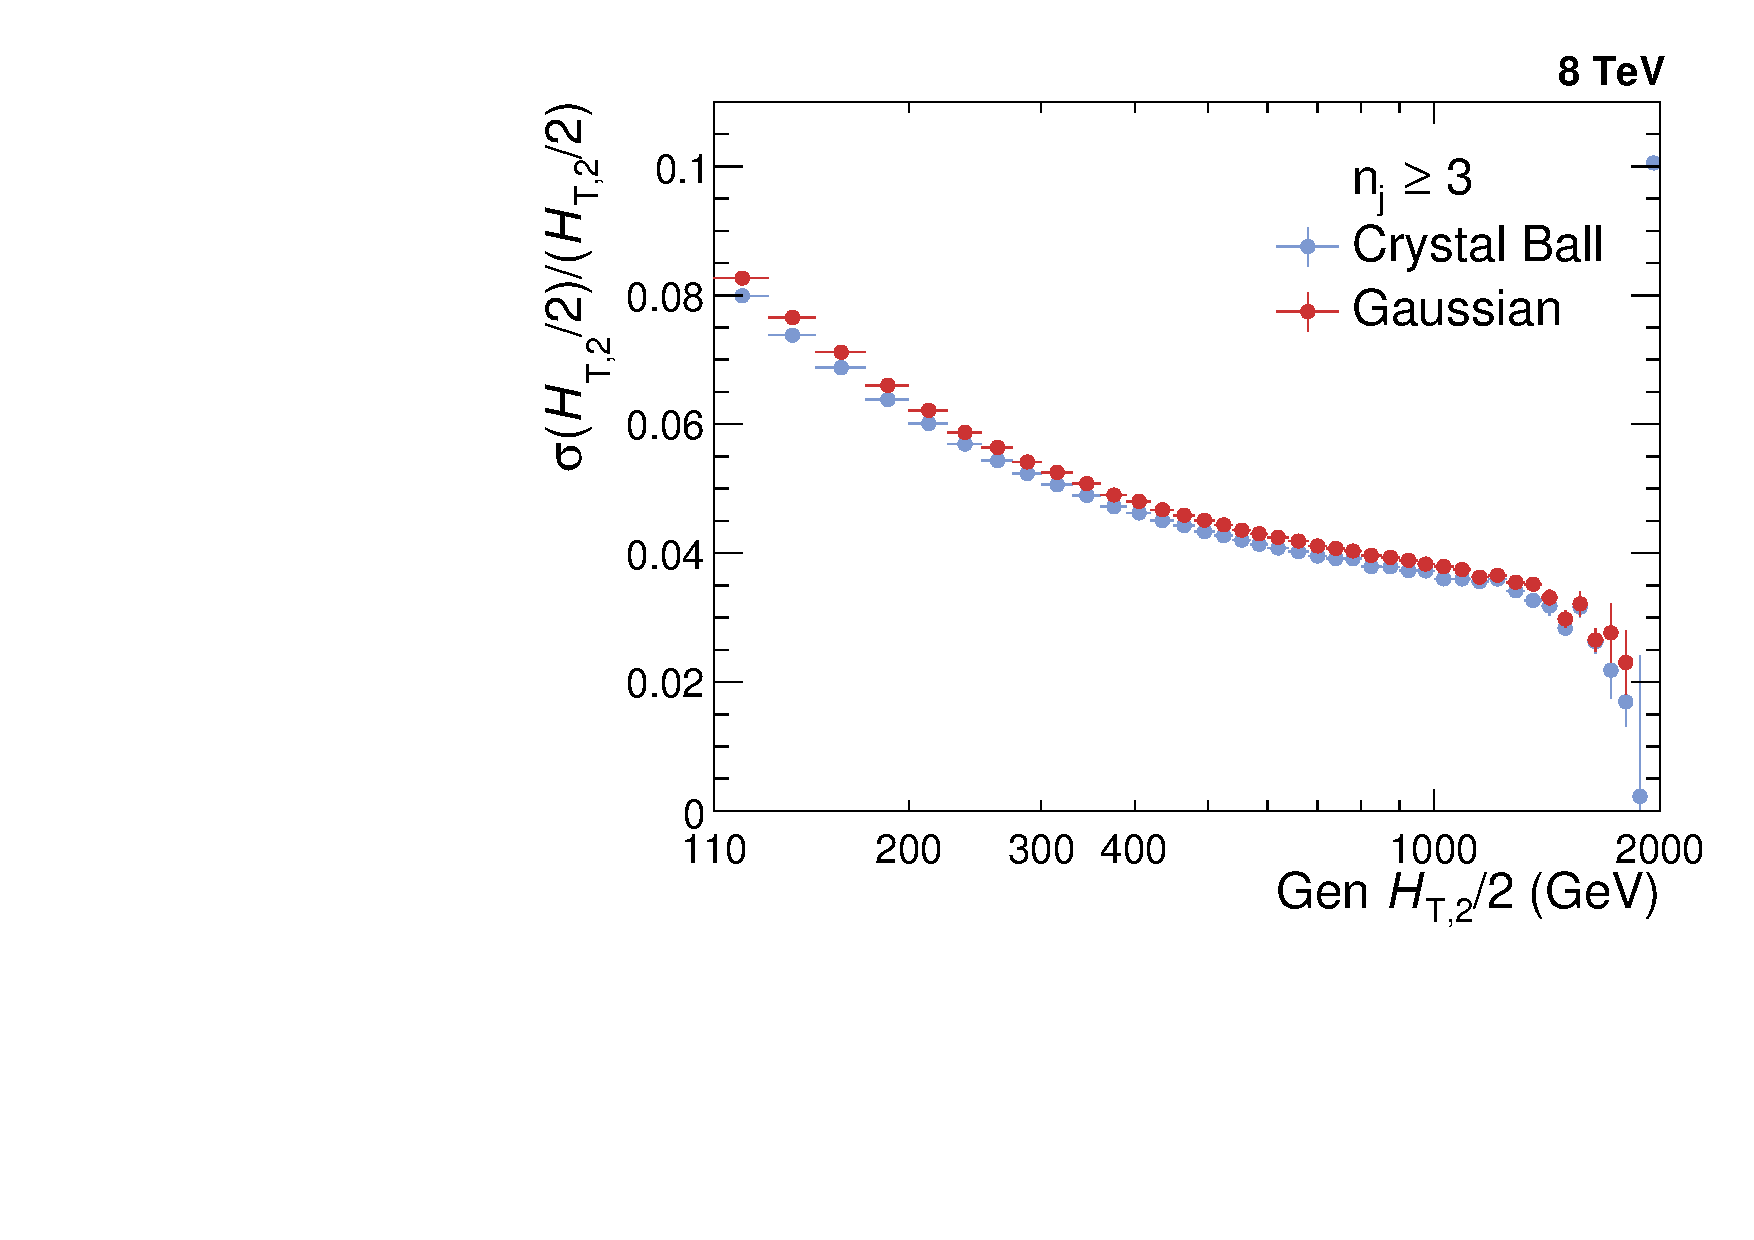
\includegraphics[width=0.51\textwidth]{Plots_HT_2_150/Comparison_Resolution_Crystal_Gauss_3.pdf}
 \caption{Comparison of jet energy resolution calculated using Crystal-Ball fit function (blue) and Gaussian fit function (red) for inclusive 2-jet events (left) and for inclusive 3-jet events (right).}
 \label{fig:res_comp}
  \end{center}
\end{figure}

\begin{figure}[!htbp]
 \begin{center}
 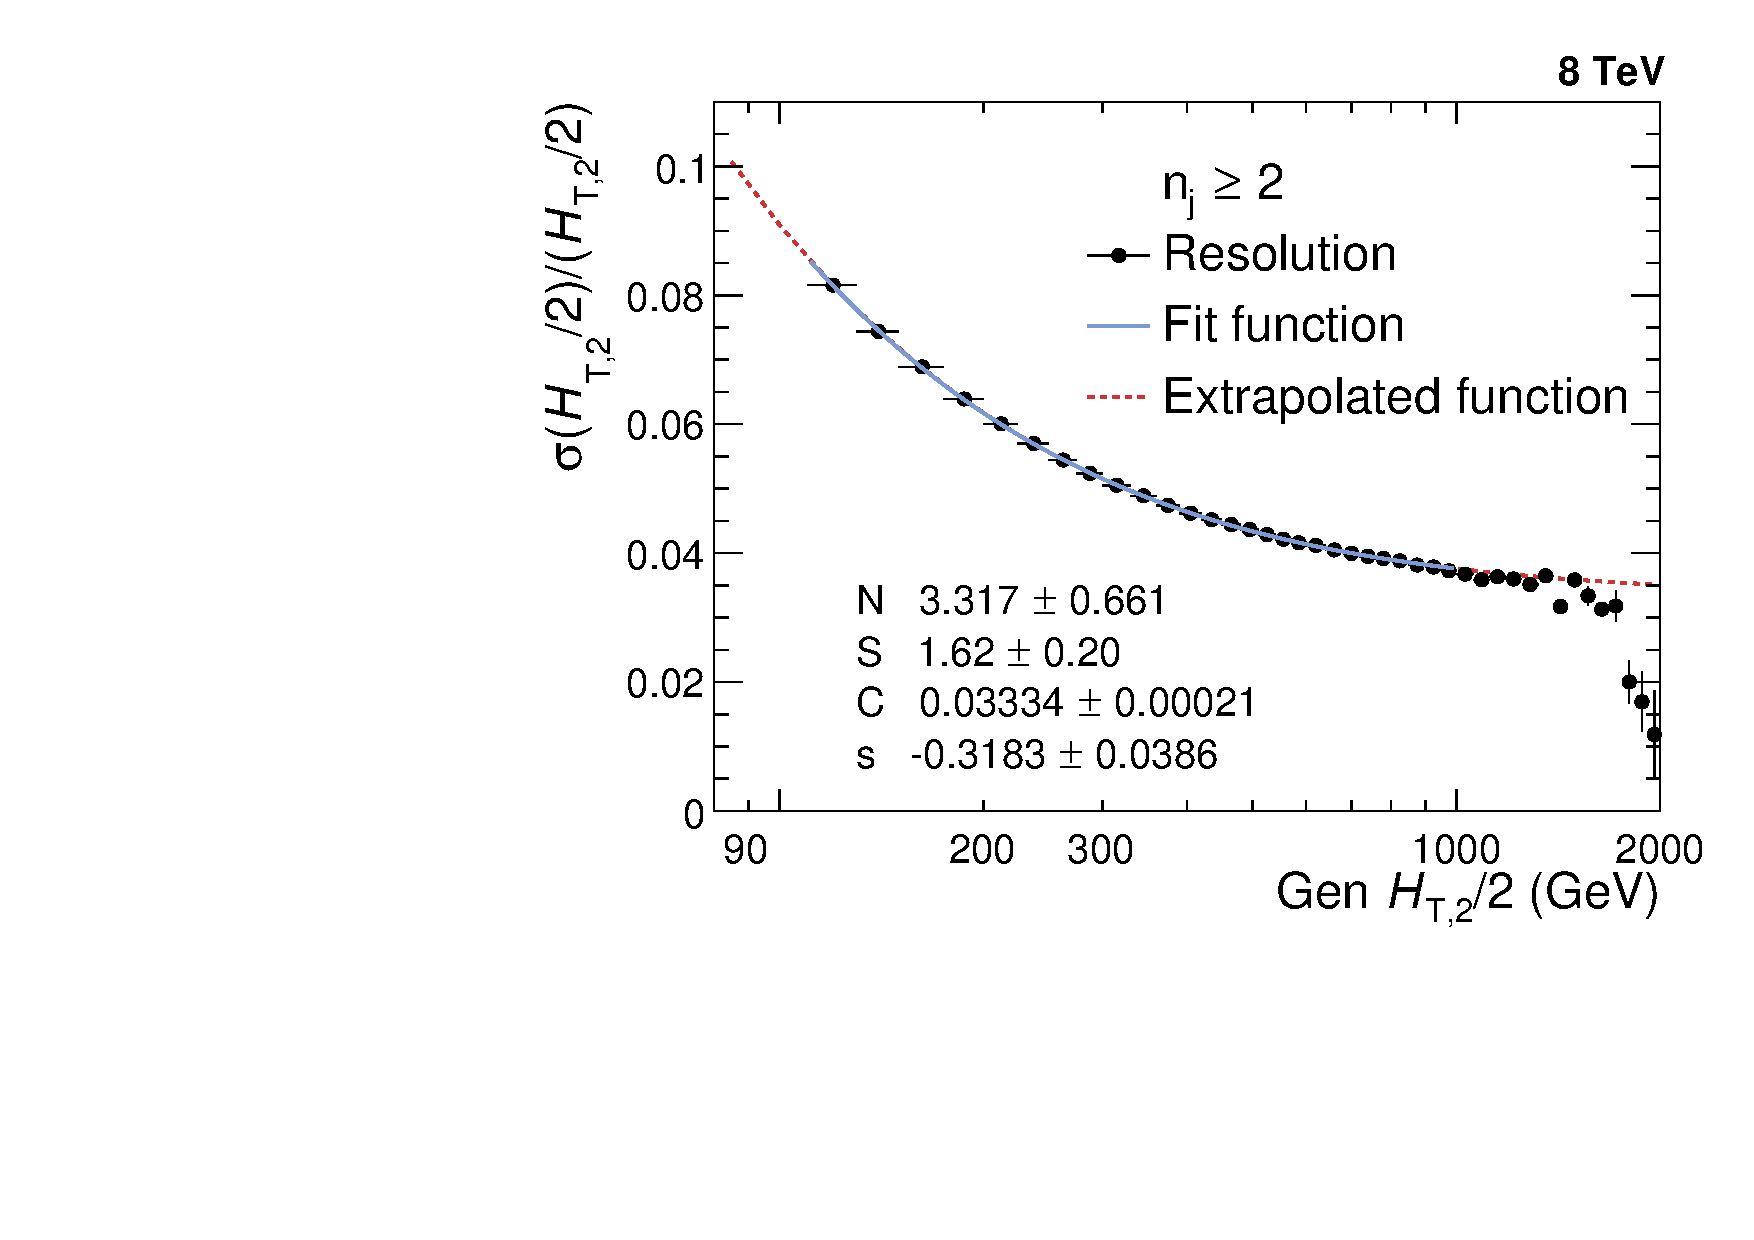
\includegraphics[width=0.51\textwidth]{Plots_HT_2_150/Extrapolate_Sigma_Value_Res_2_crystal_range_ext.pdf}%
 ~~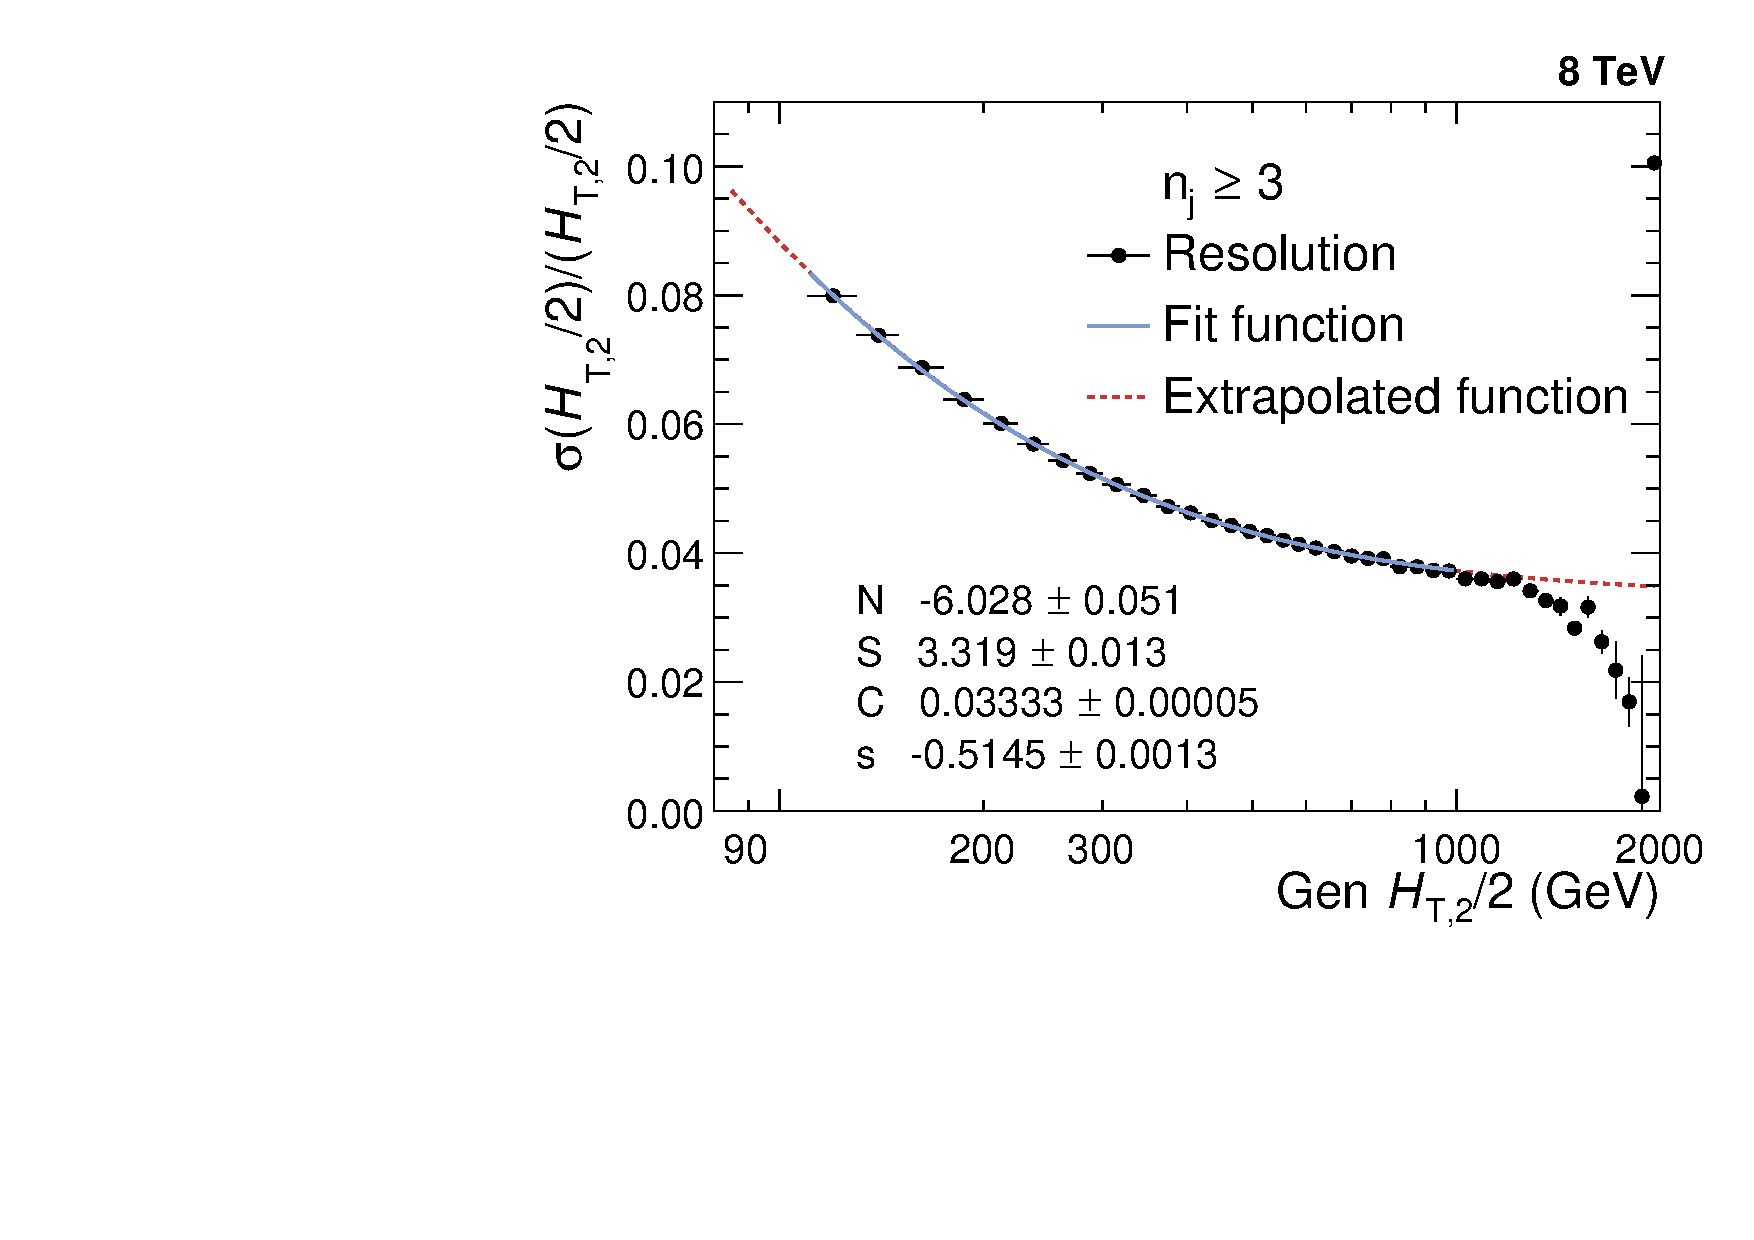
\includegraphics[width=0.51\textwidth]{Plots_HT_2_150/Extrapolate_Sigma_Value_Res_3_crystal_ext.pdf}
 \caption{Jet energy resolution (JER) is shown as a function of Gen \httwo for inclusive 2-jet events (left) and for inclusive 3-jet events (right). JER is fitted by using the modified NSC-formula (blue solid line) which is extrapolated to 80 GeV and upto 2 TeV (red dashed line) to consider the migration into lower as well as higher bins.}
    \label{fig:resolution}
  \end{center}
\end{figure}
 
Figure~\ref{fig:resolution} shows the final relative jet energy resolution (JER) which is described by a modified version of the NSC formula (blue solid line) \cite{CMS:2011esa}, as mentioned in Equation~\ref{NSC_formula}. To consider the migration to lower as well higher bins and to obtain the resolution with reasonable statistics over the full range of Gen \httwons, the fit function is extrapolated to 80 GeV and upto 2 TeV which is shown by red dashed line. The fit formula used here is based on the usual NSC formula which describes the resolution in terms of noise $N$ originating due to electronic and pileup noise and is independent of \httwons; a stochastic component $S$ due to sampling fluctuation and EM fraction fluctuation per hadrons; and a constant term $C$ because of dead material, magnetic field and calorimeter cell to cell fluctuation. In the low \httwo region the tracking has a non-negligible influence on the resolution due to the particle flow algorithm, so the additional parameter $s$ is introduced to obtain slightly better fits. The parameters obtained after fitting the relative resolution using the above mentioned NSC formula are tabulated in Table~\ref{fit_para} for \njt~and \njth~events. This calculated JER is used in unfolding procedure to smear the generated truth spectrum which is used as input in getting the response matrices and is explained in details in Sec.~\ref{sec:funcs}.

\begin{equation}
  \label{NSC_formula}
  \frac{\sigma (x)}{x} = \sqrt{sgn(N) \cdot\frac{N^{2}}{x^{2}}+S^{2}\cdot x^{s-1}+C^{2}} 
\end{equation}

\begin{table}[h]
  \centering
  \caption{The parameters obtained by fitting the relative resolution as a function of \httwo, using the modified NSC formula, for inclusive 2-jet and inclusive 3-jet events.}
  \label{fit_para}
  \vspace{2mm}
  \begin{tabular}{ccccc}
    \hline \hline
    &    N    &  S   &    C   &    s   \rbtrr \\ \hline
    Inclusive 2-jet  & ~3.32 & 1.62 & 0.0333 & -0.318  \rbtrr \\
    Inclusive 3-jet  & -6.03 & 3.32 & 0.0333 & -0.515  \rbtrr \\
    \hline \hline
  \end{tabular}
\end{table}

%Since the JER is calculated using \MGP~Reco and Gen \httwo distributions, so it is expected that the Gen \httwo smeared using this  JER should match the Reco \httwo. But this extracted JER in one large rapidity bin, smears the Gen \httwo too much because \textcolor{red}{$\rm {\frac{Smeared~Gen}{Gen}}$} does not matches with simulated \textcolor{blue}{$\rm {\frac{Reco}{Gen}}$} as observed in Fig.~\ref{fig:ratios} for \njt~(left) and \njth~(right). When the 30\% reduced JER  is used to smear Gen, then \textcolor{pink}{$\rm {\frac{Smeared~Gen}{Gen}}$} matches with simulated \textcolor{blue}{$\rm {\frac{Reco}{Gen}}$} ignoring the statistical fluctuations. So an additional unfolding uncertainty is attributed by comparison to 30\% reduced JER.  

Since the JER is calculated using \MGP~Reco and Gen \httwo distributions, so it is expected that if Gen \httwo is smeared using this JER, it should match the Reco \httwo. But this extracted JER in one large rapidity bin, smears the Gen \httwo too much because Smeared Gen/Gen ratio (red line) shows a discrepancy from simulated Reco/Gen ratio (blue line), as observed in Fig.~\ref{fig:ratios} for \njt~(left) and \njth~(right). When the 30\% reduced JER  is used to smear Gen, then the ratio Smeared Gen/Gen (pink line) matches with simulated Reco/Gen ratio (blue line) within the statistical fluctuations. Hence an additional unfolding uncertainty is attributed by comparison to 30\% reduced JER for both \njt~ and \njth~events. Due to high statistical fluctuations at high \httwo, range is presented upto 1.68 TeV only.

\begin{figure}[!htbp]
 \begin{center}
 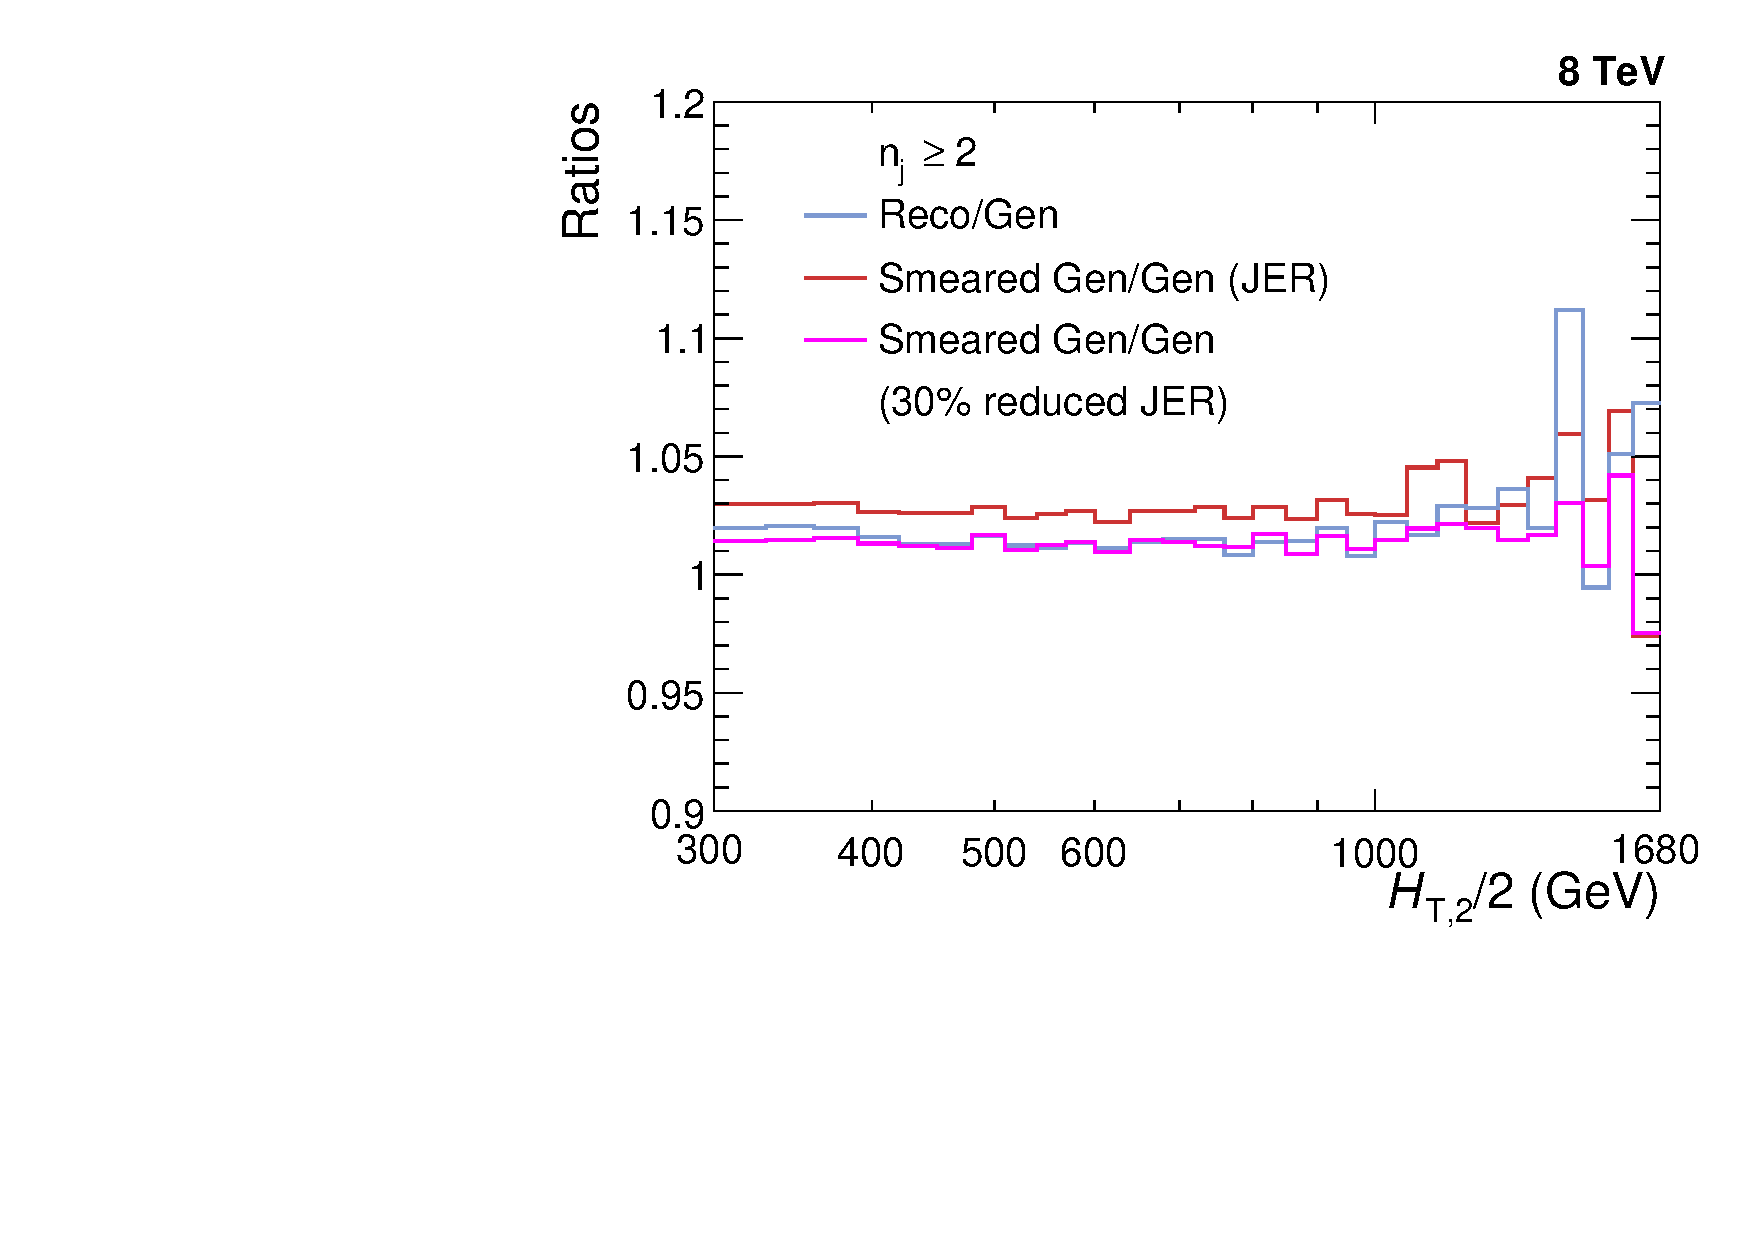
\includegraphics[width=0.51\textwidth]{Plots_HT_2_150/Ratio_Reco_2_crystal.pdf}%
 ~~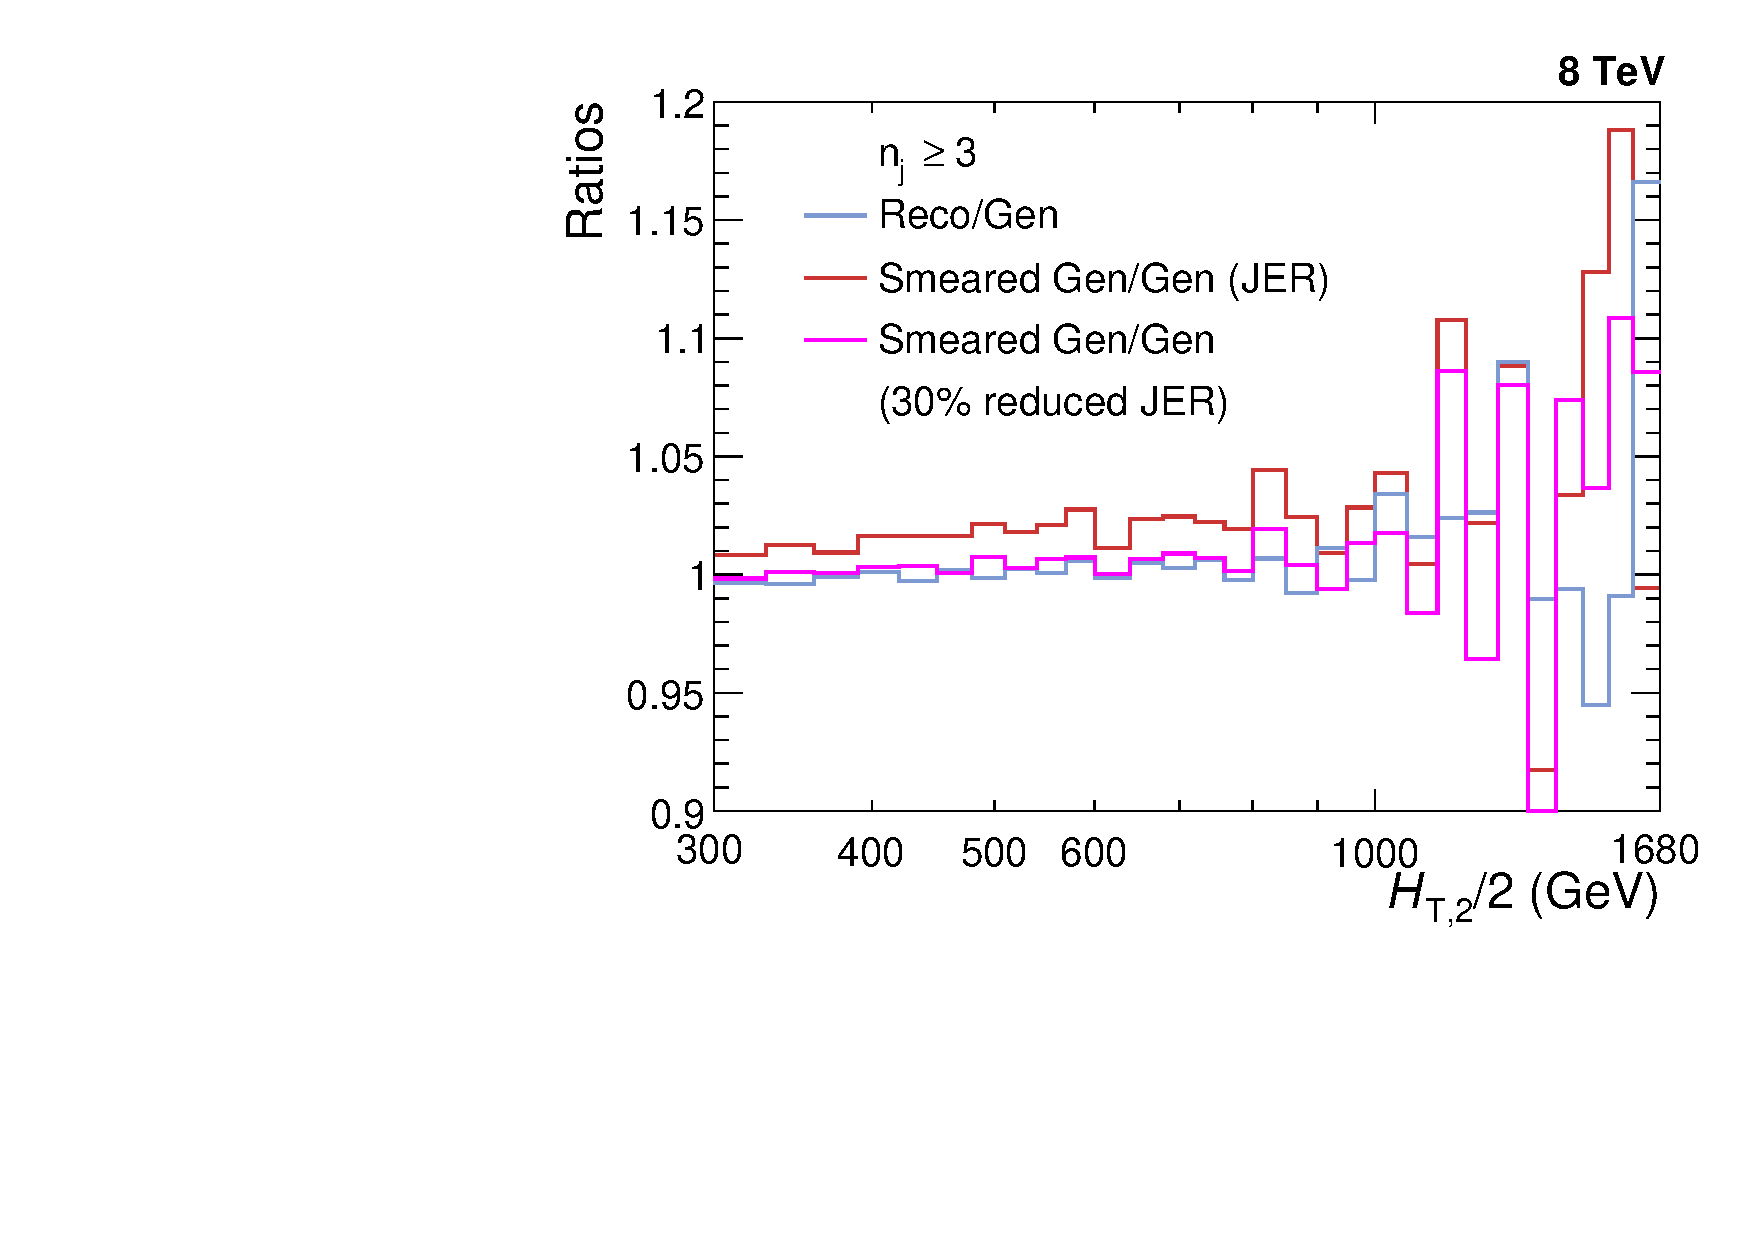
\includegraphics[width=0.51\textwidth]{Plots_HT_2_150/Ratio_Reco_3_crystal.pdf}\\
 \caption{\MadGraphF \plus \PYTHIAS Gen smeared using extracted jet energy resolution (JER) shows a discrepancy from simulated Reco as Smeared Gen/Gen ratio (red line) does not match with Reco/Gen ratio (blue line), for both inclusive 2-jet (left) and inclusive 3-jet events (right). Smeared Gen/Gen ratio (pink line) where Gen is smeared using 30\% reduced JER matches with simulated Reco/Gen ratio (blue line) within the statistical fluctuations. Hence an additional unfolding uncertainty is attributed by comparison to 30\% reduced JER.}
 \label{fig:ratios}
 \end{center}
\end{figure}

\section{Unfolding}
\label{sec:unfolding}
One of the main goals in an experimental measurement is to do the comparison between data and theory predictions or with the results from other experiments. But the finite detector resolution and the steeply falling jet \pt spectrum distorts the physical quantities. As a result, the measured observables are different from the corresponding true values. Each \pt bin content contains the migrated events from neighbouring bins along with the original events. So an unfolding process of the data should be followed in order to remove detector effects. In this analysis, the measured cross sections are corrected for detector smearing effects and unfolded to stable particle level by using the iterative D'Agostini Bayesian method \cite{DAgostini:1994fjx}, implemented in the RooUnfold software package \cite{Adye:2011gm}. The unfolding process is regularized by the number of iteration steps in this algorithm. A higher number of iterations yields a reduced \chisq but also increases the uncertainty and introduces larger bin-by-bin fluctuations and correlations. The regularization is optimized using simulated events and best results with low bin-by-bin correlations and low \chisq are achieved using four iterations in the unfolding algorithm.

\subsection{Response matrices}
\label{sec:funcs}

Unfolding uses a response matrix as an input that maps the true distribution onto the measured one. The response matrix is usually derived from simulated Monte Carlo (MC) samples, which uses as input the true distribution from MC and introduces the smearing effects by taking into account the detector resolution. Then this response matrix is used to unfold the measured data spectrum. But there are several drawbacks of constructing response matrix using this method. In some phase space regions, the shape of the distribution is not well described by the LO predictions. Also, the number of events in the MC samples are limited at high transverse momenta which introduces non-negligible statistical fluctuations in the response matrix. 

However, there is an indirect way of constructing the response matrix which uses a custom Toy Monte Carlo method. In this method, the particle level or true \httwo spectrum is obtained by fitting the theoretically predicted NLO spectrum. Then this distribution is smeared with forward smearing technique, using the extracted jet energy resolution (JER) to obtain the reconstructed level or measured \httwo spectrum. After that, the response matrix is constructed from these two distributions is used for the unfolding procedure. 

The NLO spectrum obtained from CT10-NLO PDF set is fitted with the following two different functions defined in Eq.~\ref{eq:func1} and~\ref{eq:func2}. These functions describes both the normalization and shape of the distribution.  

\begin{itemize}
\item {\bf Function I : }
  %\end{itemize} 

  \begin{equation}
    \label{eq:func1}
    f(\httwo) = N[x_{T}]^{-a}[1-x_{T}]^{b} \times exp[-c/x_{T}]
  \end{equation}
  where N is normalization factor and a, b, c are fit parameters.\\

  This function is derived from the below function \cite{CMS:2011ab} :
  \begin{equation}
    \label{eq:funcderive}
    f(p_{T};\alpha,\beta,\gamma) = N_{0}[p_{T}]^{-\alpha}\bigg[1-\frac{2~p_{T}~cosh(y_{min})}{\sqrt{s}}\bigg]^{\beta} \times exp[-\gamma/p_{T}]
  \end{equation}
  using 
  \begin{equation}
    \alpha = a,~~\beta = b,~~\gamma = c*\sqrt{s}/2, \\
    x_{T} = \frac{2*\httwons *cosh(y_{min})}{\sqrt{s}} = \frac{2*\httwons}{\sqrt{s}}
  \end{equation}
  where transverse scaling variable $x_{T}$ corresponds to the proton fractional momentum $x$ for dijets with rapidity $y$ = 0, $\sqrt{s}$ = 8000 GeV and $y_{min}$ is low-edge of the rapidity bin $y$ under consideration (here $y_{min}$ is taken equal to 0)
  
\item {\bf Function II : }

  \begin{equation}
    \label{eq:func2}
    f(H_{T,2}/2) = A_{0}\Big(1-\frac{H_{T,2}/2}{A_{6}}\Big)^{A_{7}} \times 10^{F(\httwo)}, {\rm where} ~~~{F(x) = \sum\limits_{i=1}^5 A_{i}\Big(log\big(\frac{x}{A_{6}}\big)\Big)^{i}}
  \end{equation}

  where the parameter $A_{6}$ is fixed to $\frac{\sqrt{s}}{2~cosh(y_{min})}$, where $\sqrt{s}$ = 8000 GeV and $y_{min}$ is 
  the minimum rapidity. The other parameters are derived from the fitting.
\end{itemize}

\begin{figure}[h]
  \begin{center}
    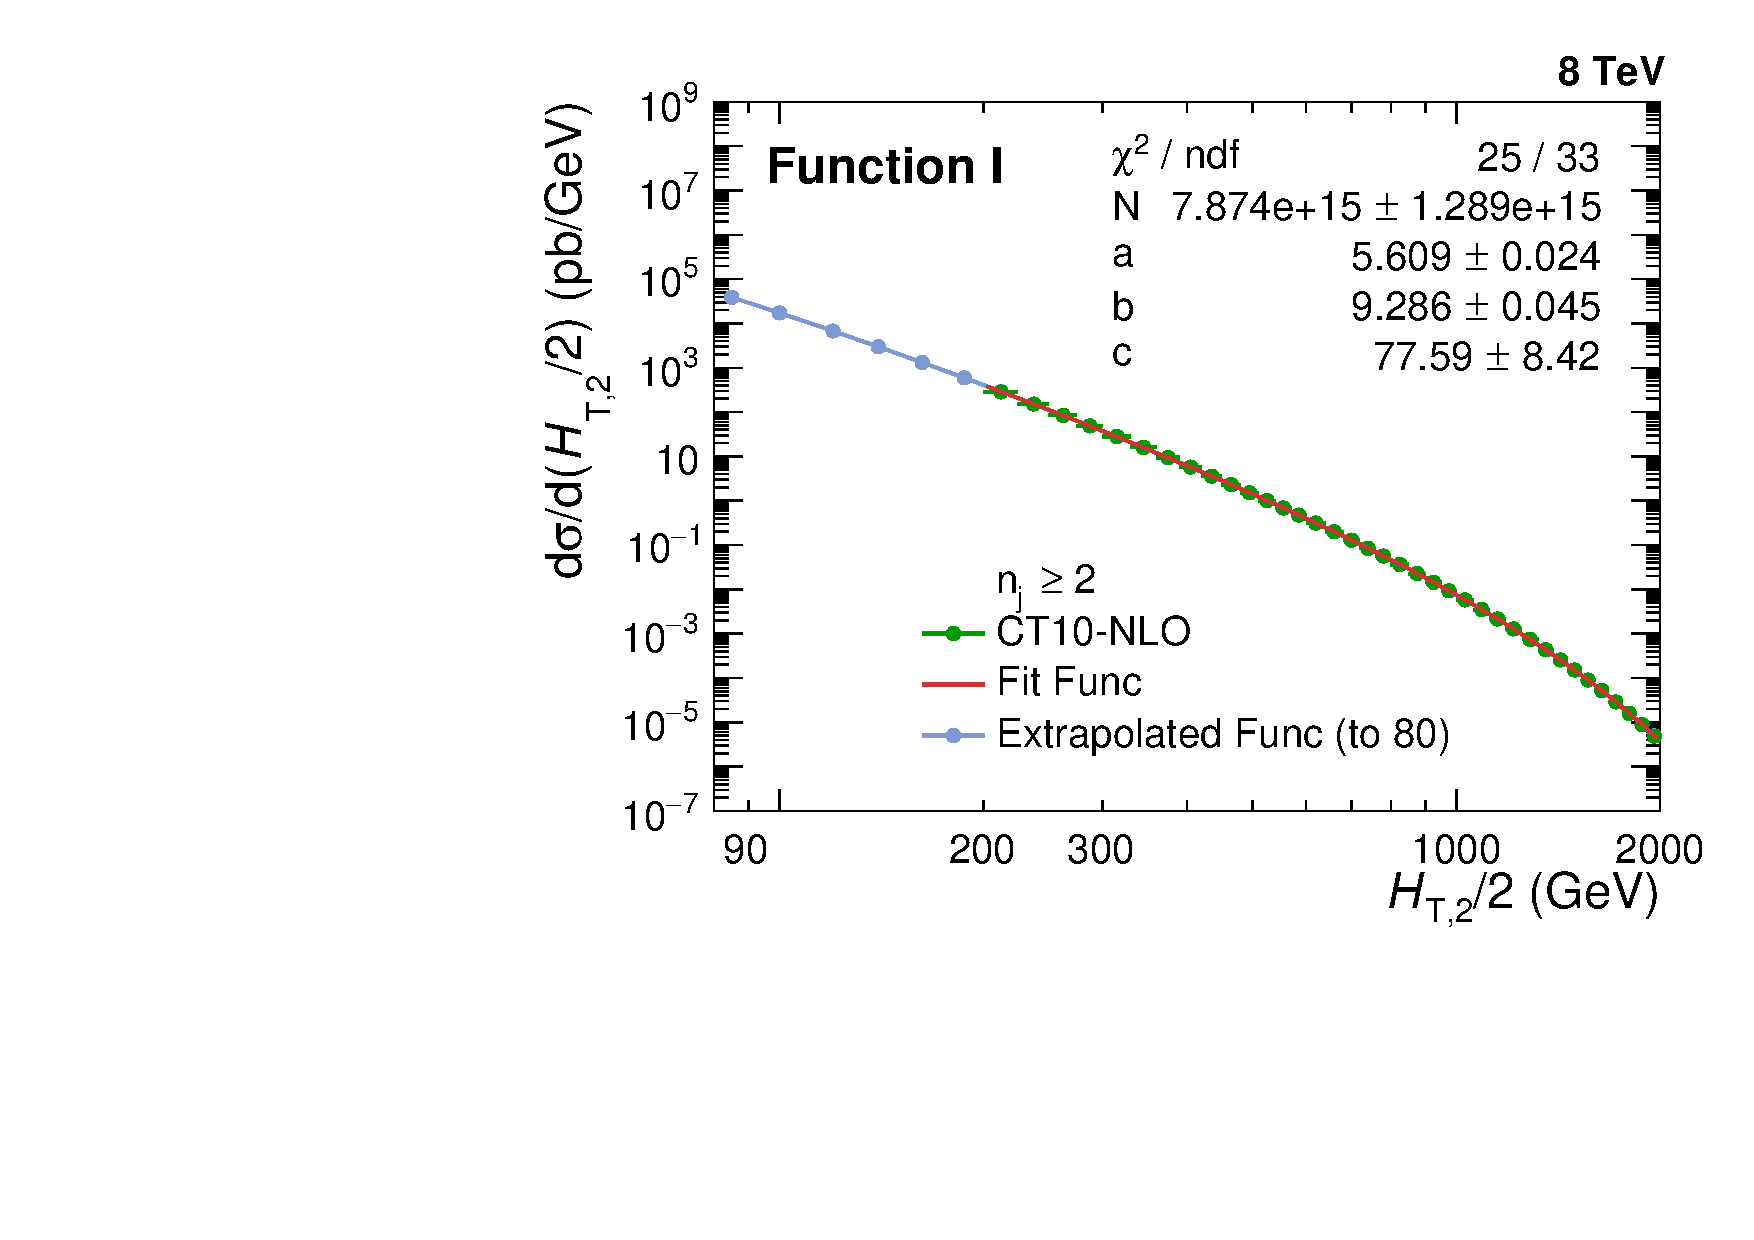
\includegraphics[width=0.51\textwidth]{Plots_HT_2_150/Extrapolate_Theory_2_HT_2_150_funcI.pdf}%
    ~~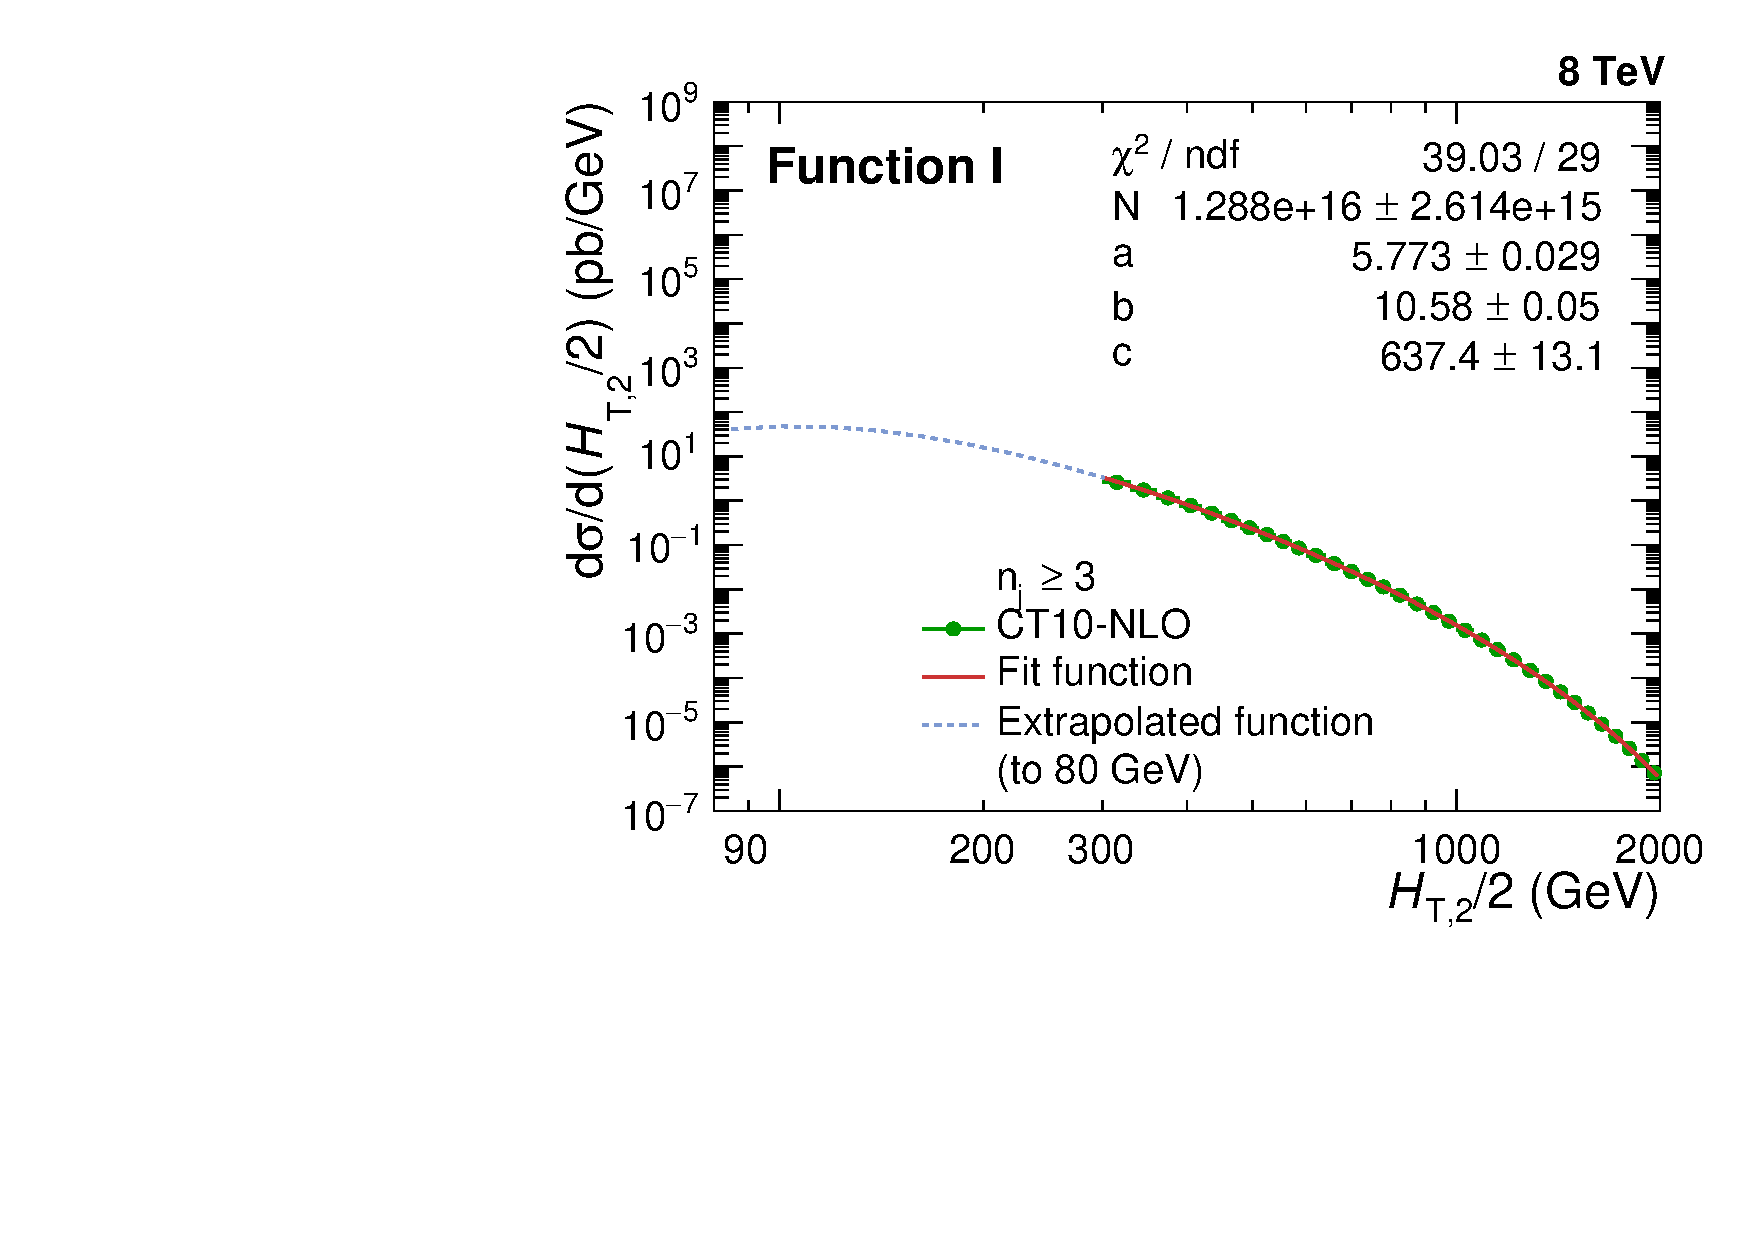
\includegraphics[width=0.51\textwidth]{Plots_HT_2_150/Extrapolate_Theory_3_HT_2_150_funcI.pdf}\\
    \vspace{5mm}
    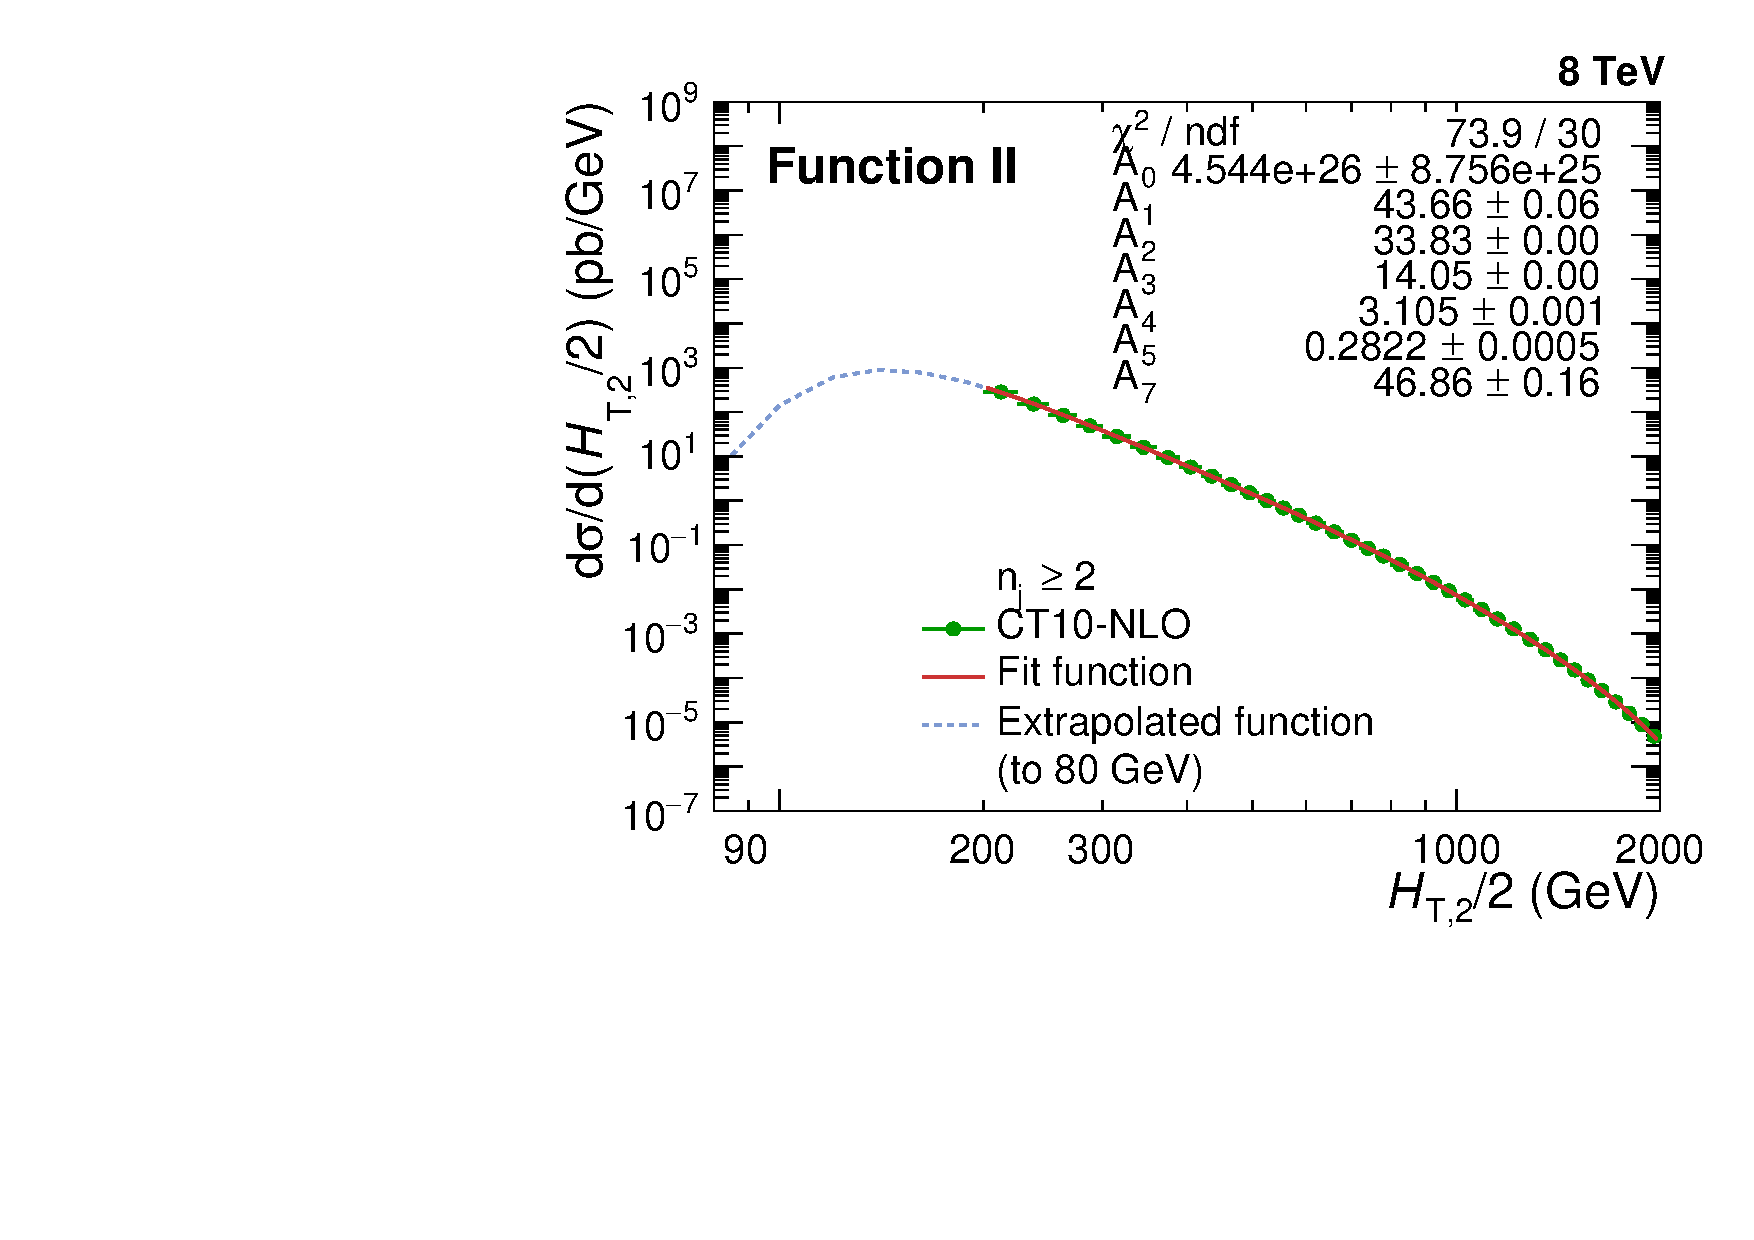
\includegraphics[width=0.51\textwidth]{Plots_HT_2_150/Extrapolate_Theory_2_HT_2_150_funcII.pdf}%
    ~~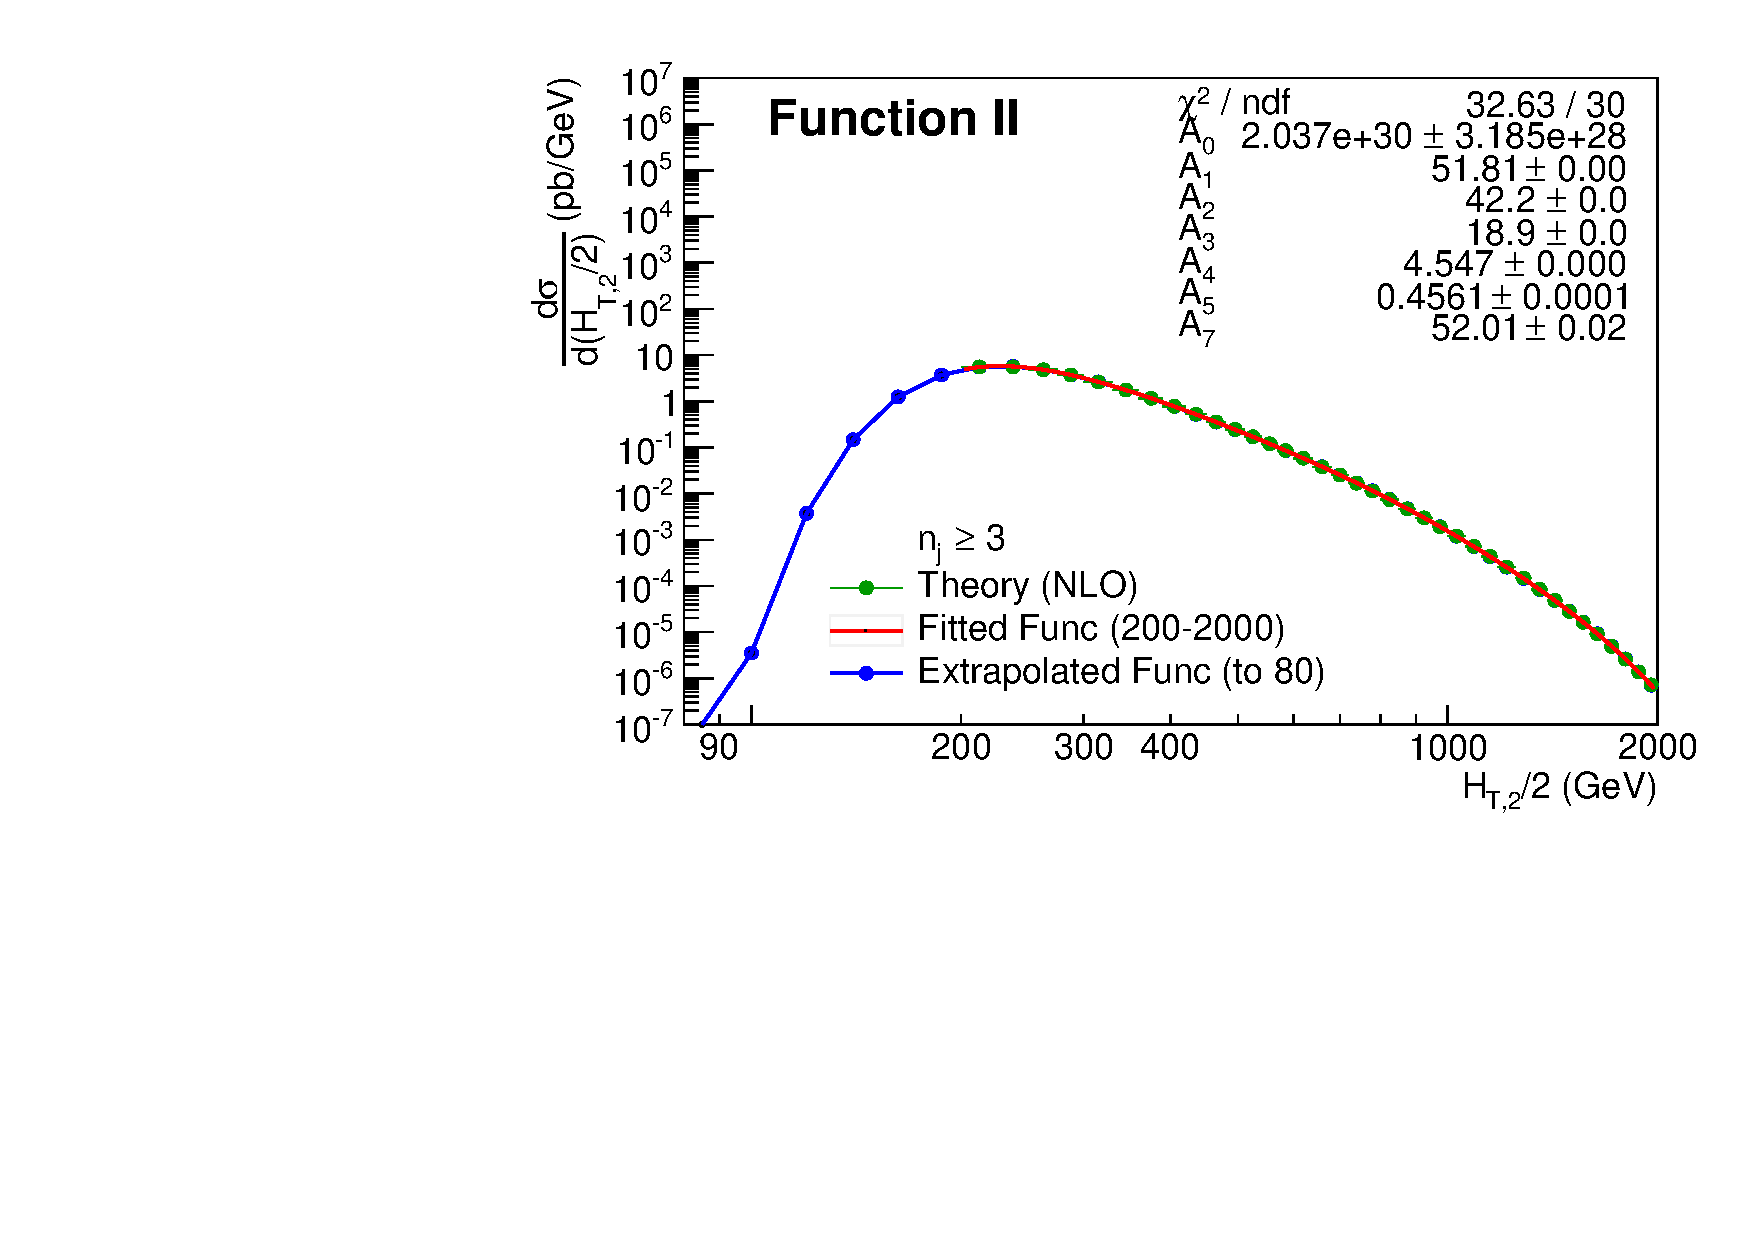
\includegraphics[width=0.51\textwidth]{Plots_HT_2_150/Extrapolate_Theory_3_HT_2_150_funcII.pdf}\\
    \caption{Fitted CT10-NLO spectrum of differential cross section as a function of \httwo (green solid circles) using Function I (top) defined in Eq.~\ref{eq:func1} and using Function II (bottom) given by Eq.~\ref{eq:func2}, for inclusive 2-jet events (left) and for inclusive 3-jet events (right). To consider the migration to lower \httwo bins, the fit functions described by red lines are extrapolated to 80 GeV (blue dashed lines).}
    \label{fig:fit}
  \end{center}
\end{figure}

Figure~\ref{fig:fit} shows the fitted CT10-NLO spectrum of differential cross section as a function of \httwo (green solid circles) using Function I (top) and using Function II (bottom) : for inclusive 2-jet events (left) and for inclusive 3-jet events (right). Function I is used primarily to generate response matrices and perform the closure tests and Function II is used as an alternative function to calculate unfolding uncertainty, described in Sec.~\ref{sec:unfolding_unc}. To include the migration to lower bins, the fit functions described by red lines are extrapolated to 80 GeV (blue dashed lines).

A flat \httwo spectrum is generated by using toy Monte Carlo events and the fit parameters obtained from the NLO spectrum using function I (as shown in Fig.~\ref{fig:fit}) provides weights to the flat spectrum. A total of ten million events are generated randomly (in \httwo range 80-2000). These generated values are then smeared with a Gaussian function, where $\sigma$ of the Gaussian is determined from the relative resolution parametrization as a function of \httwo calculated from NSC formula mentioned in equation~\ref{NSC_formula}. The parameters N, S, C used for smearing are taken from Table~\ref{fit_para}. These randomly generated (Gen$_{\rm Toy}$) and smeared (Measured$_{\rm Toy}$) values are used to fill the response matrices. Figure~\ref{fig:response_NLO} shows the response matrices derived using the Toy MC for \njt~(left) and \njth~events (right). The matrices are normalized to the number of events in each column. The response matrices are diagonal with small off-diagonal migrations between close-by \httwo bins.

\begin{figure}[!htbp]
 \begin{center}
 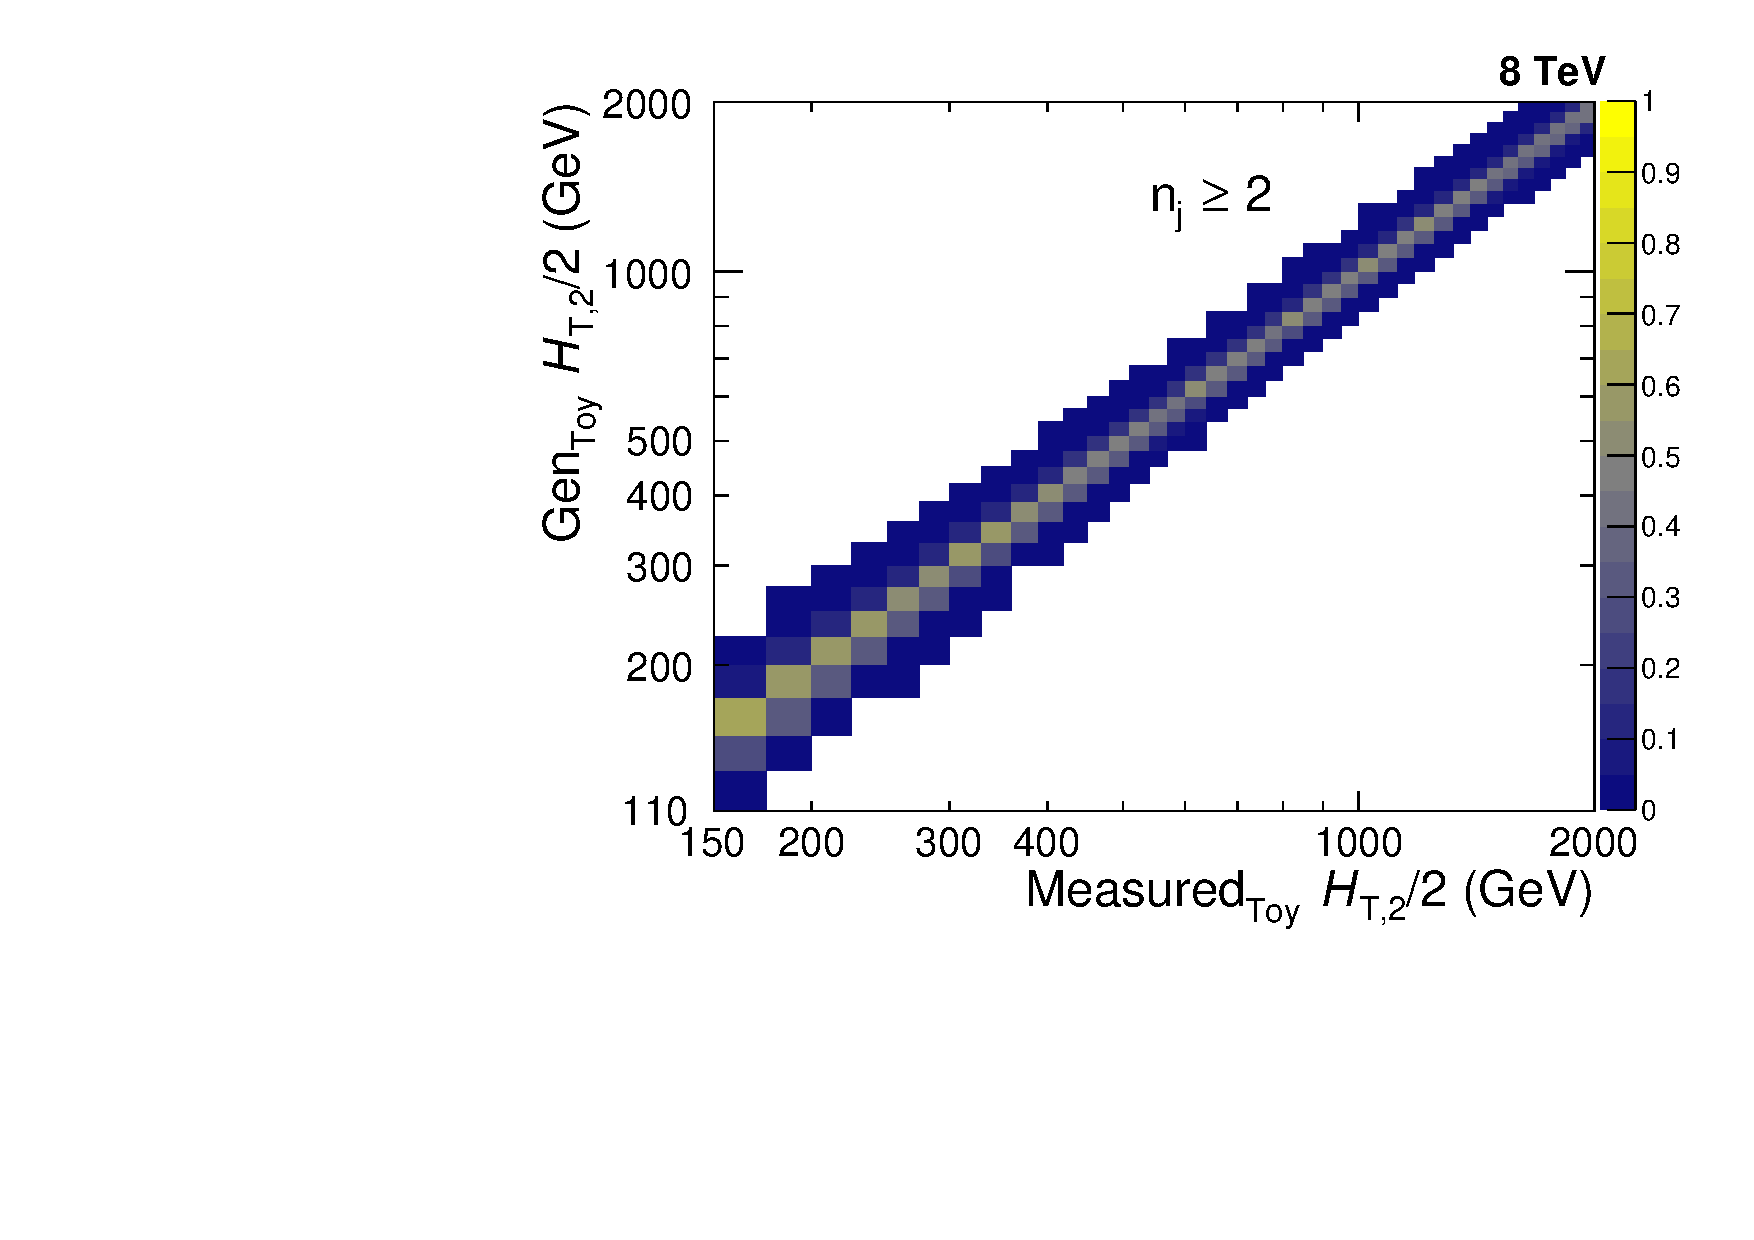
\includegraphics[width=0.51\textwidth]{Plots_HT_2_150/Normalized_Response_Matrix_NLO_2_range_column.pdf}%
 ~~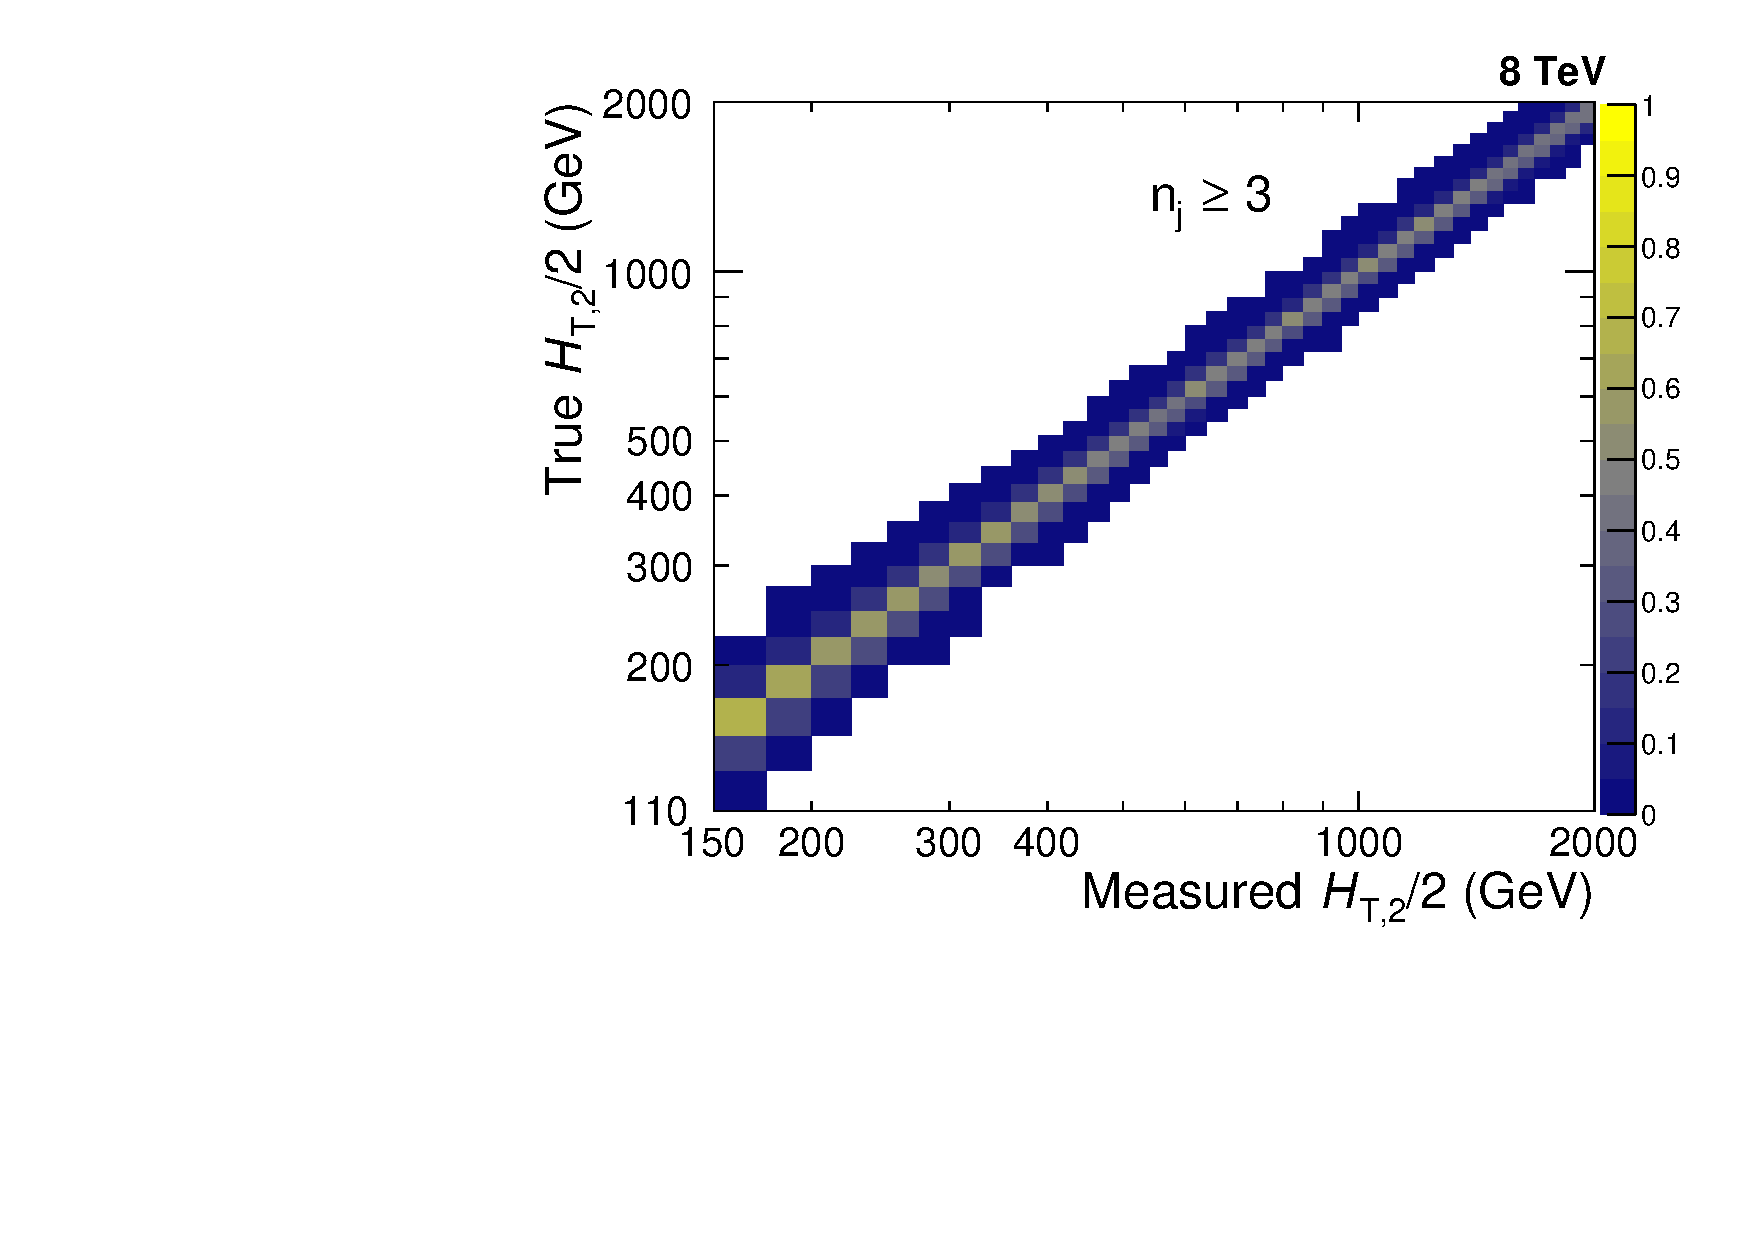
\includegraphics[width=0.51\textwidth]{Plots_HT_2_150/Normalized_Response_Matrix_NLO_3_column.pdf} 
 \caption{The response matrices are derived using the Toy Monte Carlo and forward smearing method, for inclusive 2-jet (left) and inclusive 3-jet events (right). The matrices are normalized to the number of events in each column and are diagonal with small off-diagonal migrations between close-by \httwo bins.}
 \label{fig:response_NLO}
 \end{center}
\end{figure}

\subsection{Closure test}
A closure test has been performed to confirm the working of the unfolding procedure. In this test, Measured$_{\rm Toy}$ spectrum is unfolded using the constructed response matrices shown in Figure~\ref{fig:response_NLO}. It is expected that the same Gen$_{\rm Toy}$  spectrum should be re-obtained after unfolding. Figure~\ref{fig:unfolded_smeared} shows that the unfolded Measured$_{\rm Toy}$ spectrum, matches exactly with Gen$_{\rm Toy}$ spectrum as the ratio of these distributions is perfectly flat at one for both \njt~(left) and \njth~events (right).

For another closure test, Reco \MGP~MC differential cross section distribution is unfolded using the above constructed response matrices using JER for forward smearing the randomly generated spectrum. While taking ratio of the unfolded distribution to that of Gen \MGP~MC, it is observed that a well closure is not obtained. This is represented by blue line in Fig.~\ref{fig:unfolded_reco_NLO} for \njt~(left) and \njth~(right). As observed in Fig.~\ref{fig:ratios} in Sec.~\ref{sec:Resolution}, if Reco \MGP~MC is unfolded using the response matrices obtained using 30\% reduced JER, then the good closure is obtained as shown by red line in Fig.~\ref{fig:unfolded_reco_NLO}.

\begin{figure}[h]
 \begin{center}
 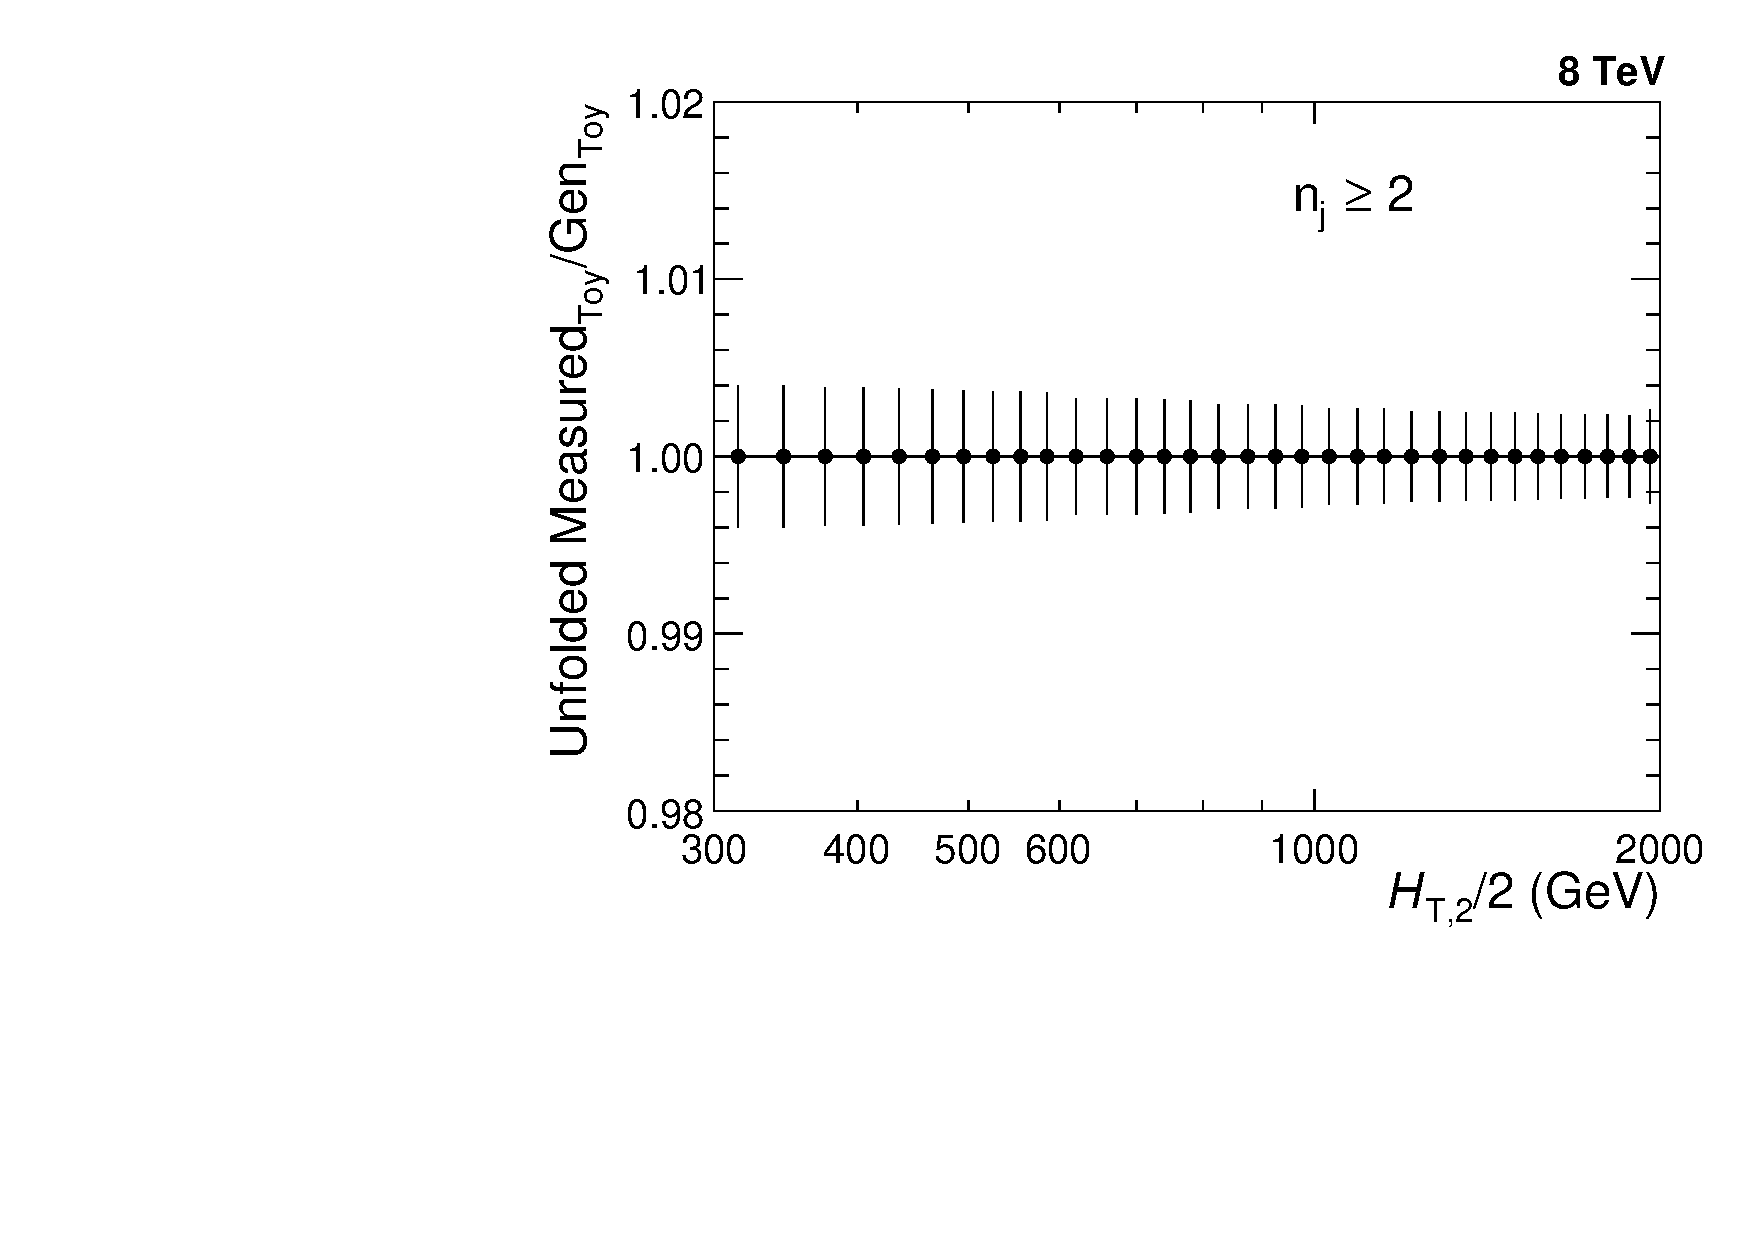
\includegraphics[width=0.51\textwidth]{Plots_HT_2_150/Ratio_Unfolding_NLO_2_funcI.pdf}%
 ~~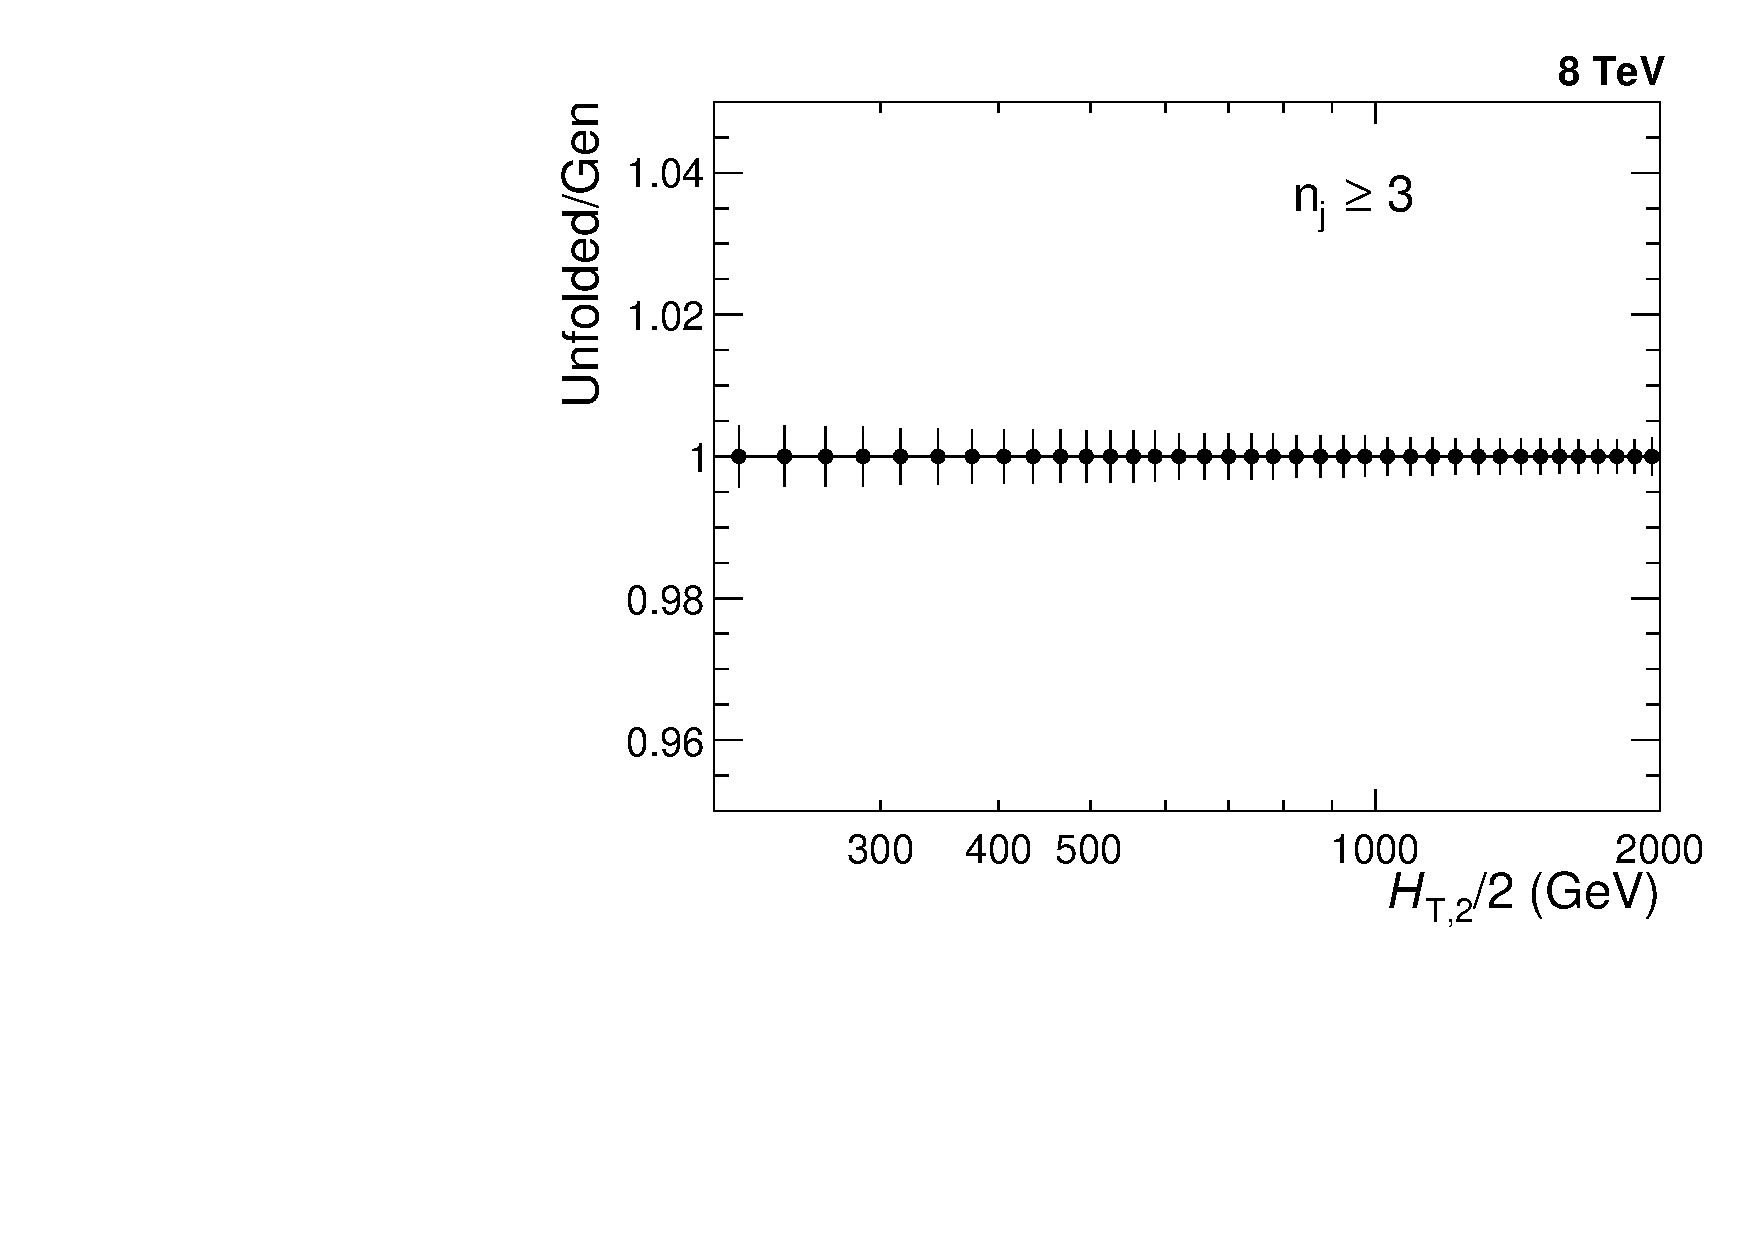
\includegraphics[width=0.51\textwidth]{Plots_HT_2_150/Ratio_Unfolding_NLO_3_funcI.pdf}
 \caption{Closure test of the unfolding technique where the smeared spectrum obtained from Toy Monte Carlo method (Measured$_{\rm Toy}$), is unfolded using the constructed response matrices (obtained by forward smearing the randomly generated spectrum (Gen$_{\rm Toy}$) using extracted jet energy resolution (JER)). As expected, the unfolded Measured$_{\rm Toy}$ spectrum matches exactly with Gen$_{\rm Toy}$ spectrum as the ratio of these distributions is perfectly flat at one for both \njt~(left) and \njth~events (right).}
 \label{fig:unfolded_smeared}
 \end{center}
\end{figure}

\begin{figure}[!htp]
 \begin{center}
 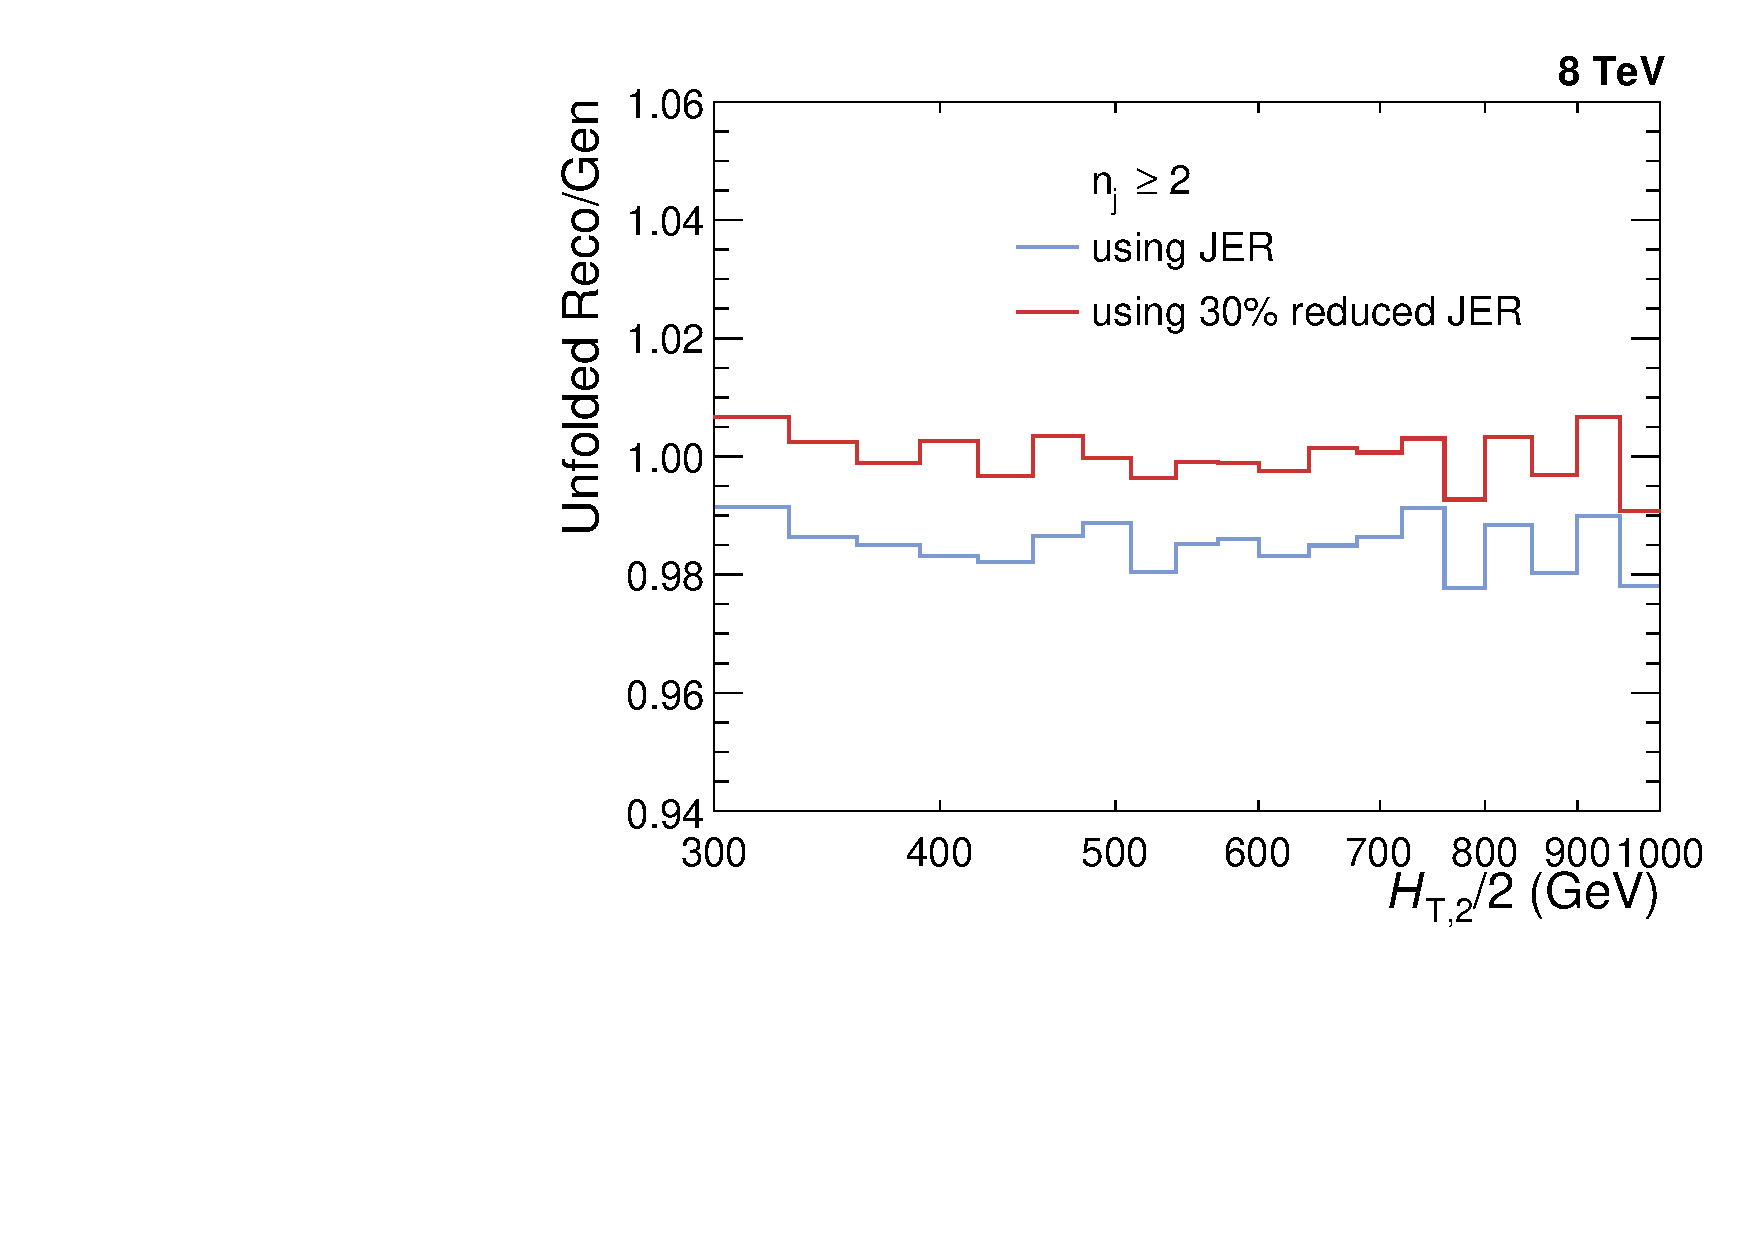
\includegraphics[width=0.51\textwidth]{Plots_HT_2_150/Comparison_closure_2_range.pdf}%
 ~~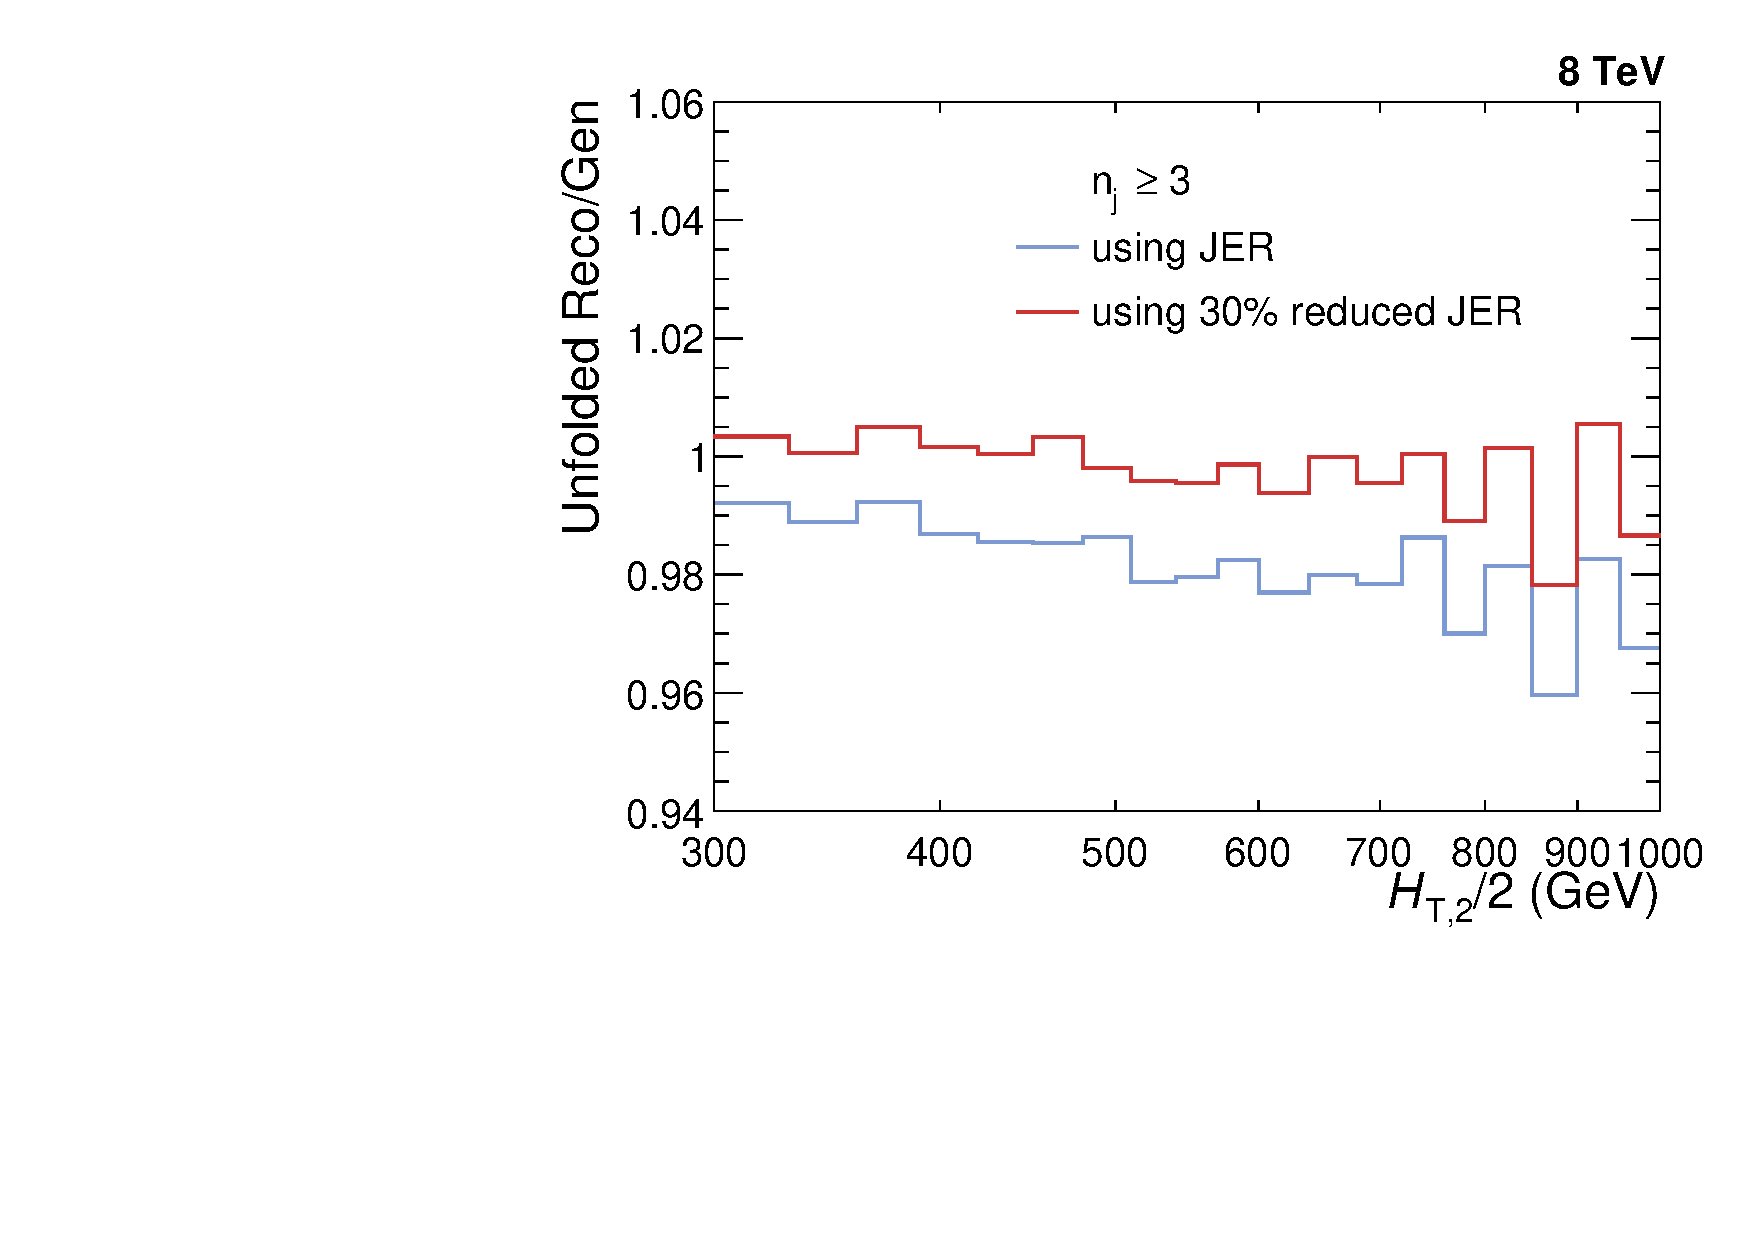
\includegraphics[width=0.51\textwidth]{Plots_HT_2_150/Comparison_closure_3.pdf}
 \caption{Reco \MadGraphF \plus \PYTHIAS Monte Carlo (\MGP~MC) differential cross section distributions unfolded with the response matrices (obtained by forward smearing the randomly generated spectrum (Gen) using extracted jet energy resolution (JER)), does not give a good closure with Gen \MGP~MC (blue line), for inclusive 2-jet (left) and inclusive 3-jet events (right). After performing the unfolding using 30\% reduced JER, a good closure is obtained (red line).}
 \label{fig:unfolded_reco_NLO}
 \end{center}
\end{figure}

\subsection{Unfolding measurement}
After validity the unfolding method, the measured differential cross sections as a function of \httwo are unfolded using the above reconstructed response matrices. The unfolded data spectrum is compared to that of measured one in Fig.~\ref{fig:unfolded_data} for \njt~(left) and \njth~(right). As already discussed that 30\% reduced JER gives better closures than JER, so the unfolding of data is done with response matrices using JER (blue) as well as 30\% reduced JER (red). The difference between both is taken as an additional uncertainty on the unfolded measurement. %The unfolding does not working well for bins near to minimum \pt cut for inclusive 2-jet events because two-jet rate is very sensitive to soft gluon emission while the higher jet multiplicities are less affected. %The event yield for each bin in \httwo is tabulated in Appendix in Table~\ref{table_event}. 

\begin{figure}[!htp]
 \begin{center}
 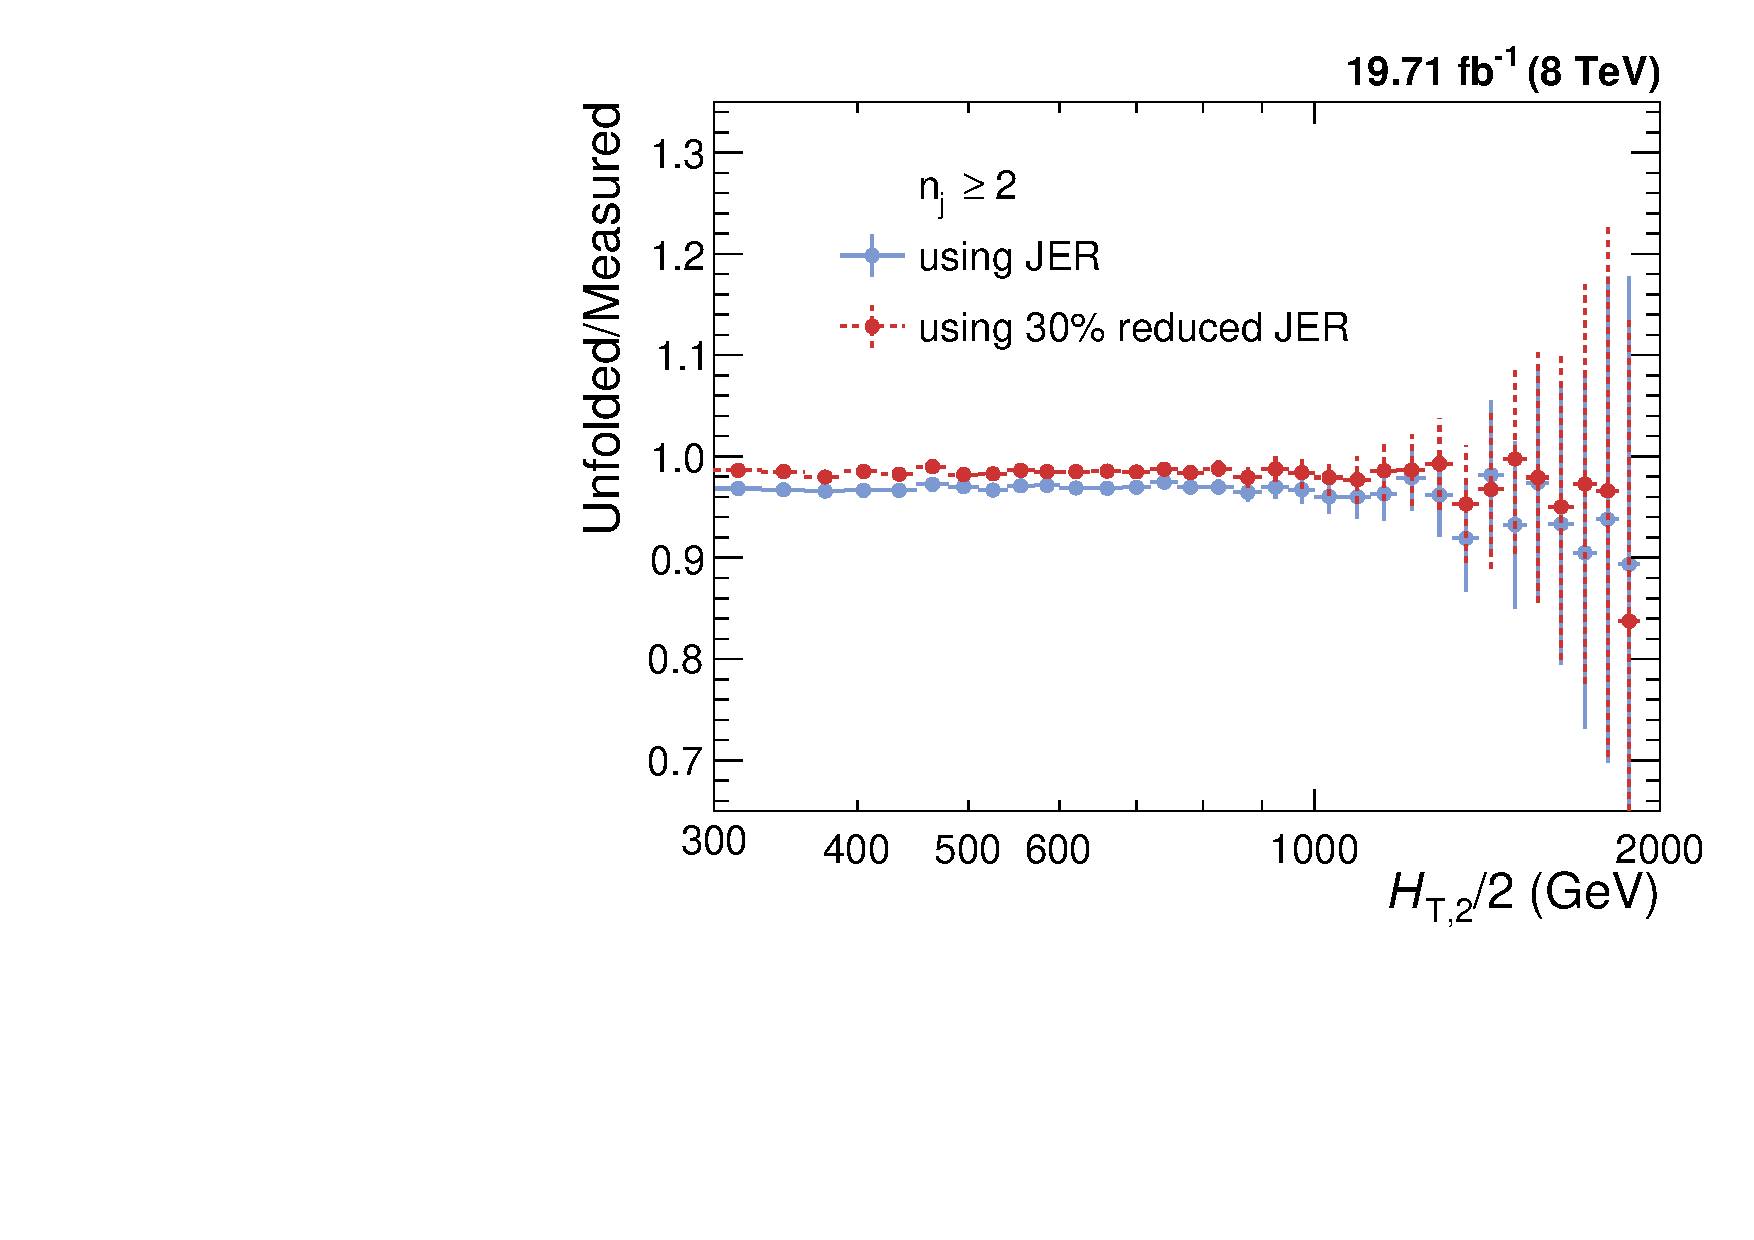
\includegraphics[width=0.51\textwidth]{Plots_HT_2_150/Ratio_Unfolding_data_NLO_2.pdf}%
 ~~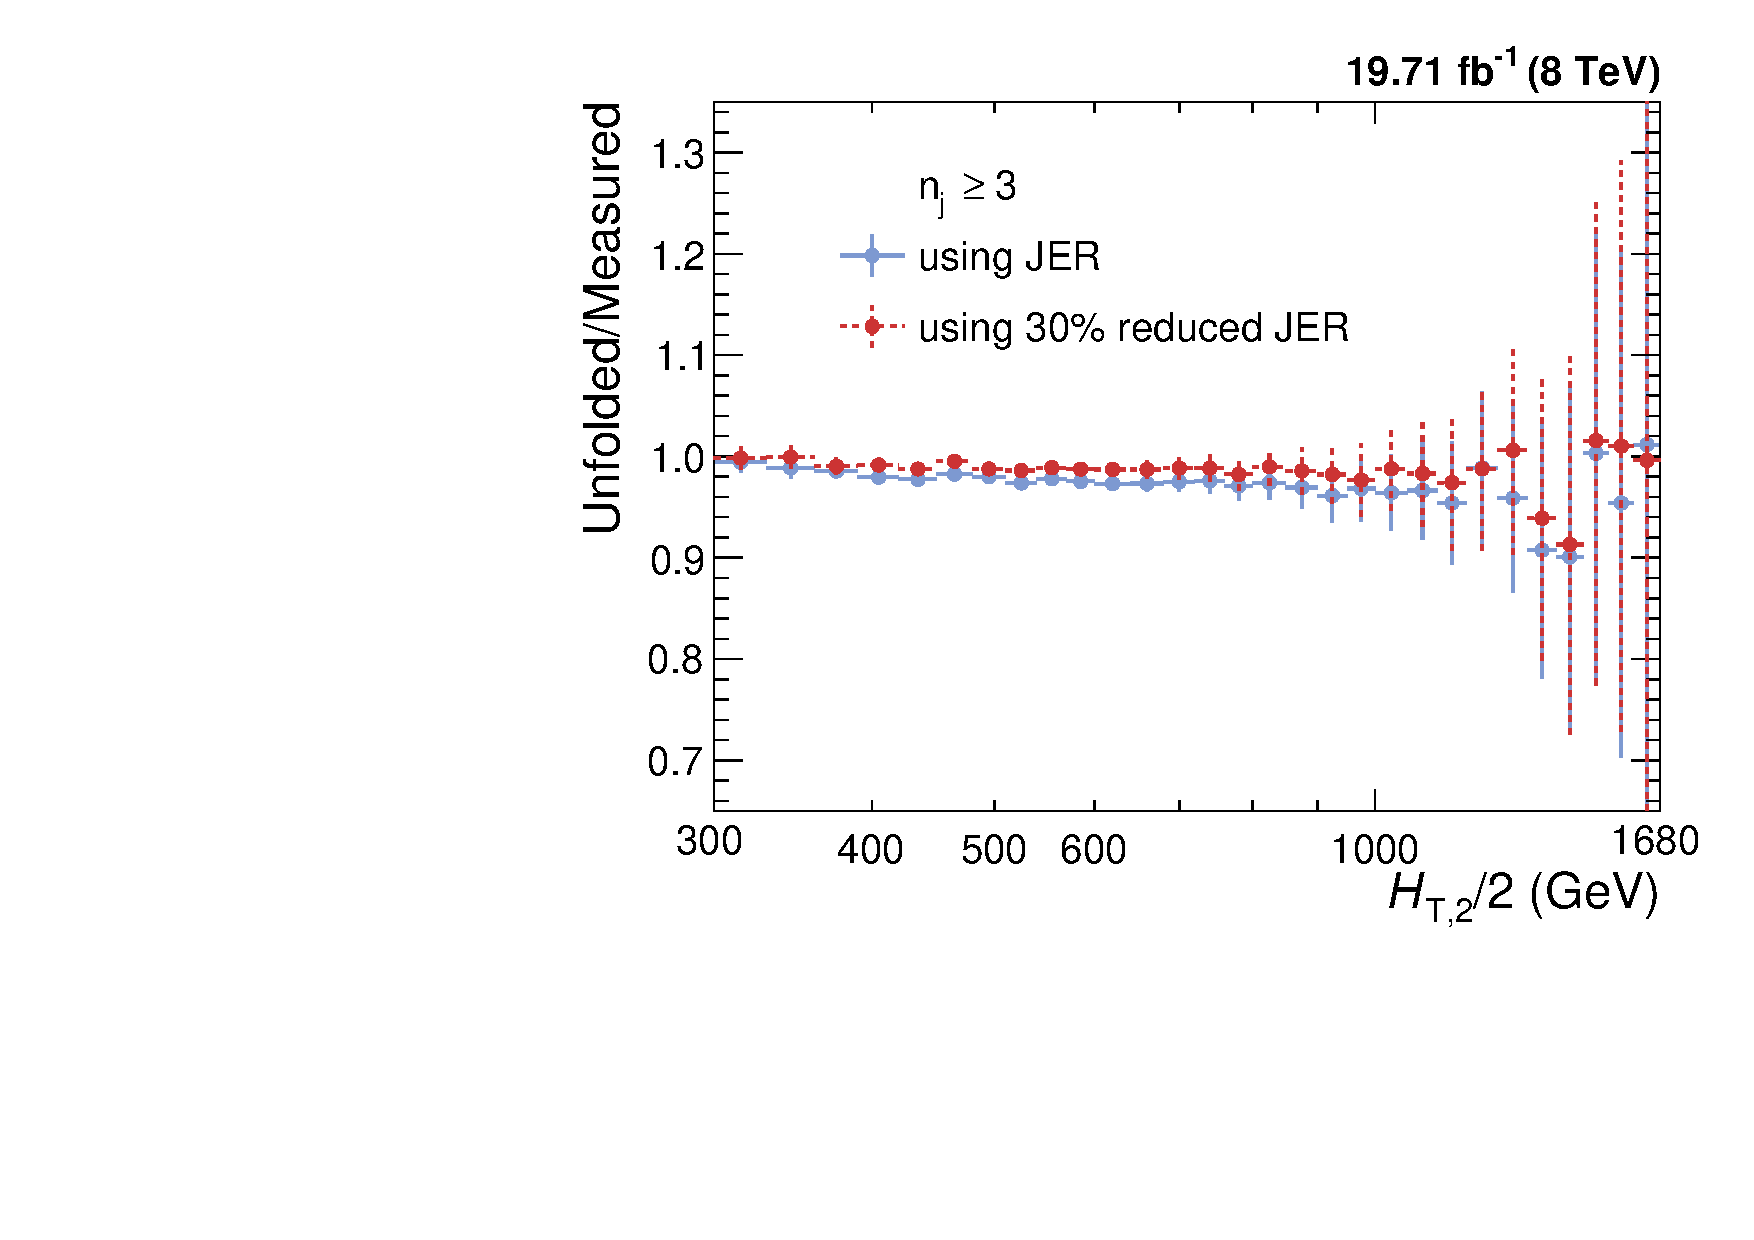
\includegraphics[width=0.51\textwidth]{Plots_HT_2_150/Ratio_Unfolding_data_NLO_3.pdf}
 \caption{The unfolded differential cross sections as a function of \httwo are compared with that of the measured one for inclusive 2-jet (left) and inclusive 3-jet events (right). The unfolding is done with response matrices using JER (blue) as well as 30\% reduced JER (red). The difference between both is taken as an additional uncertainty on the unfolded measurement.}
 \label{fig:unfolded_data}
 \end{center}
\end{figure}

\section{Experimental uncertainties}
\label{sec:exp_unc}
In an experimental measurement of any physical observable, the uncertainties play a key role and hence are important to study in a physics analysis. The uncertainties are of two types : statistical and systematic. The statistical uncertainties arise due to random fluctuations depending on the number of selected events. The systematic uncertainties may be due to known detector effects, model dependence, assumptions
made or various corrections applied. The statistical and systematic errors can in general be added in quadrature, if uncorrelated. In this section, all the experimental uncertainties affecting the cross section measurement are described.

 \subsection{Luminosity measurement uncertainty}
The LHC luminosity delivered to CMS in the 2012 proton-proton physics run is measured  by using the silicon pixel cluster counting method \cite{CMS:2013gfa}. The uncertainty related to the integrated luminosity measurement for the 2012 LHC run is estimated to be 2.5\% (syst.) and 0.5\% (stat.). The luminosity uncertainty propagates directly to any absolute cross section measurement. Hence, a combined systematic uncertainty of 2.6\% is assigned which is fully correlated across all the \httwo bins. 

\subsection{Statistical uncertainty}
\label{sec:unfolding_stat}
Statistical uncertainty on the measurement is propagated through the unfolding using a toy MC technique. The measured data points are smeared within their statistical uncertainties and the unfolding procedure is repeated multiple times for each smeared spectra. One million of such toy spectra are used to propagate the statistical uncertainty. The statistical uncertainty slightly increases during the unfolding process which can be seen in Fig.~\ref{fig:stat_unc} where the relative statistical uncertainty before (blue line) and after (red line) unfolding procedure is shown for \njt~(left) and \njth~ events (right). 

\begin{figure}[h]
 \begin{center}
 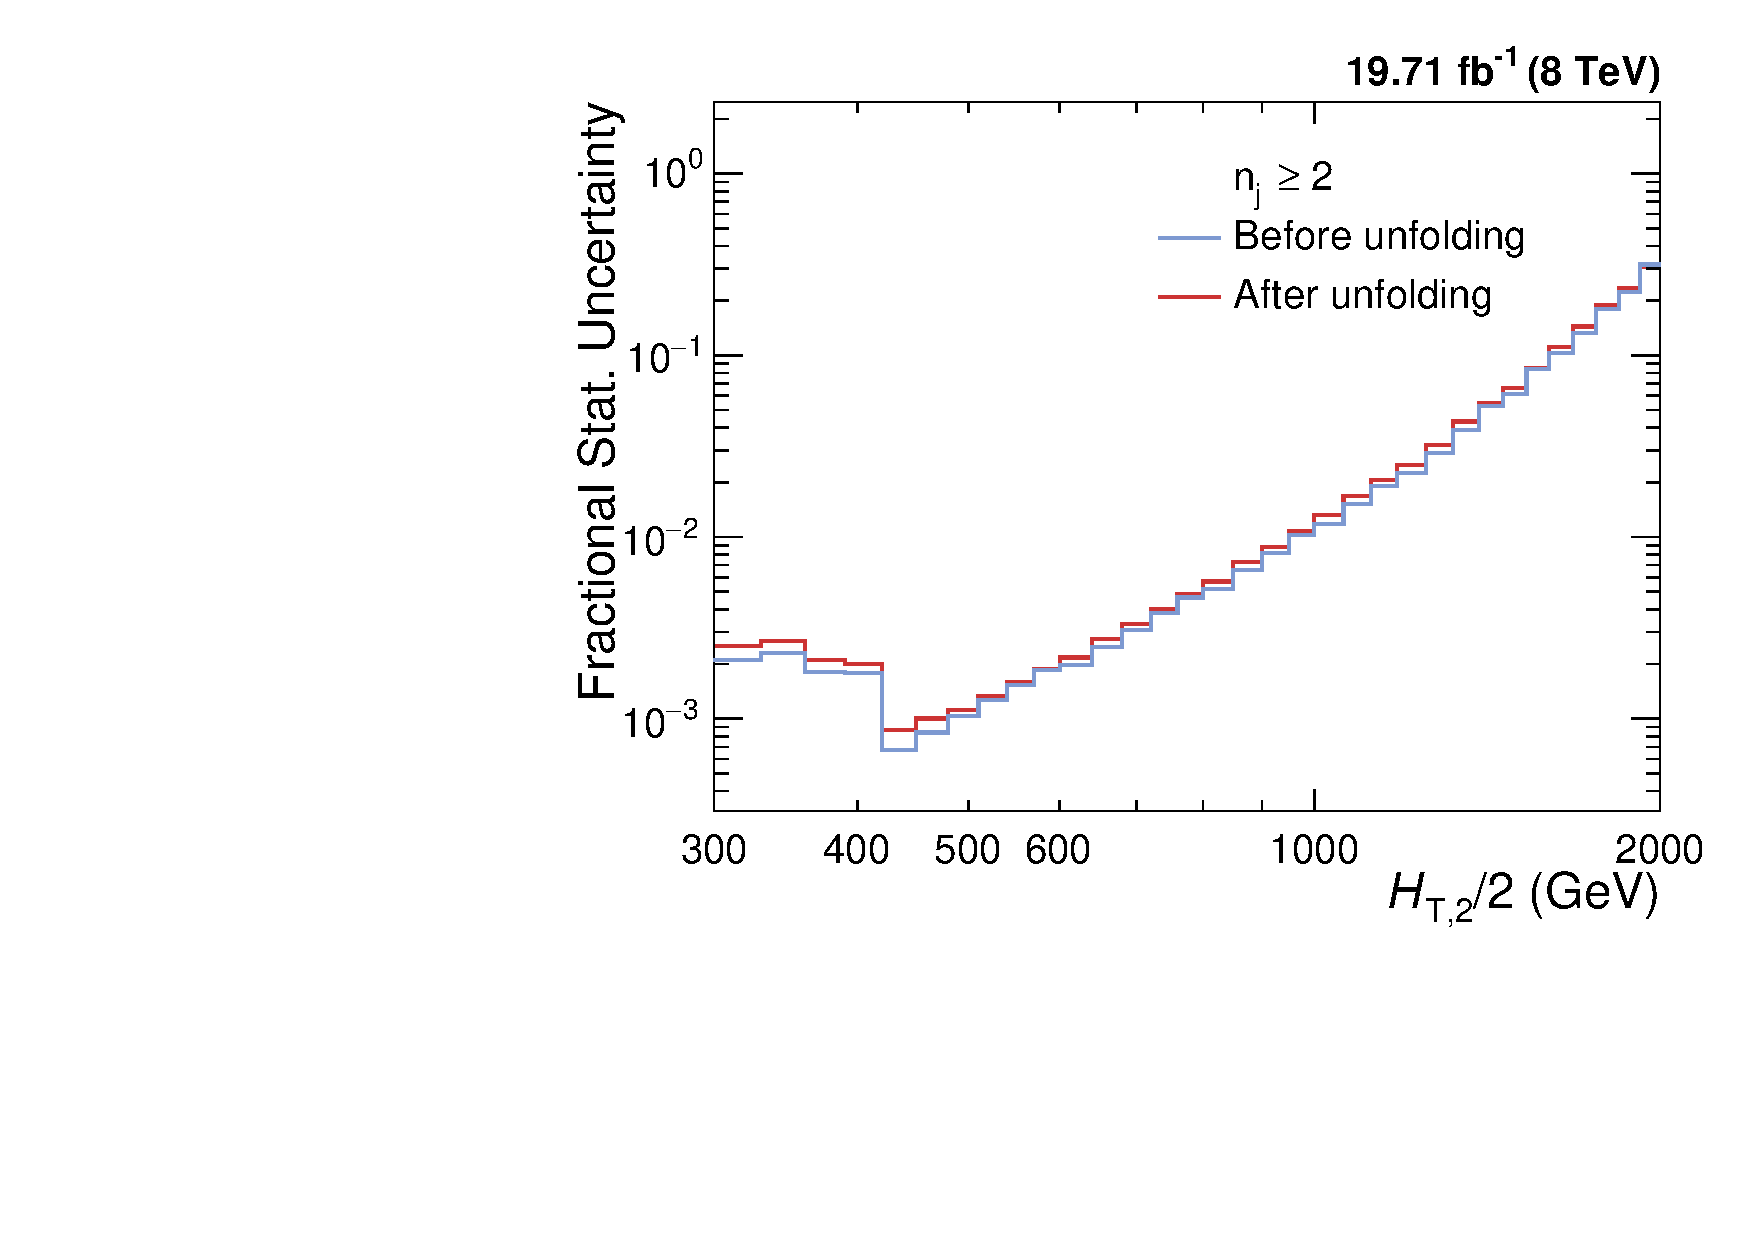
\includegraphics[width=0.51\textwidth]{Plots_HT_2_150/Comparison_stat_unc_2_HT_2_150.pdf}%
 ~~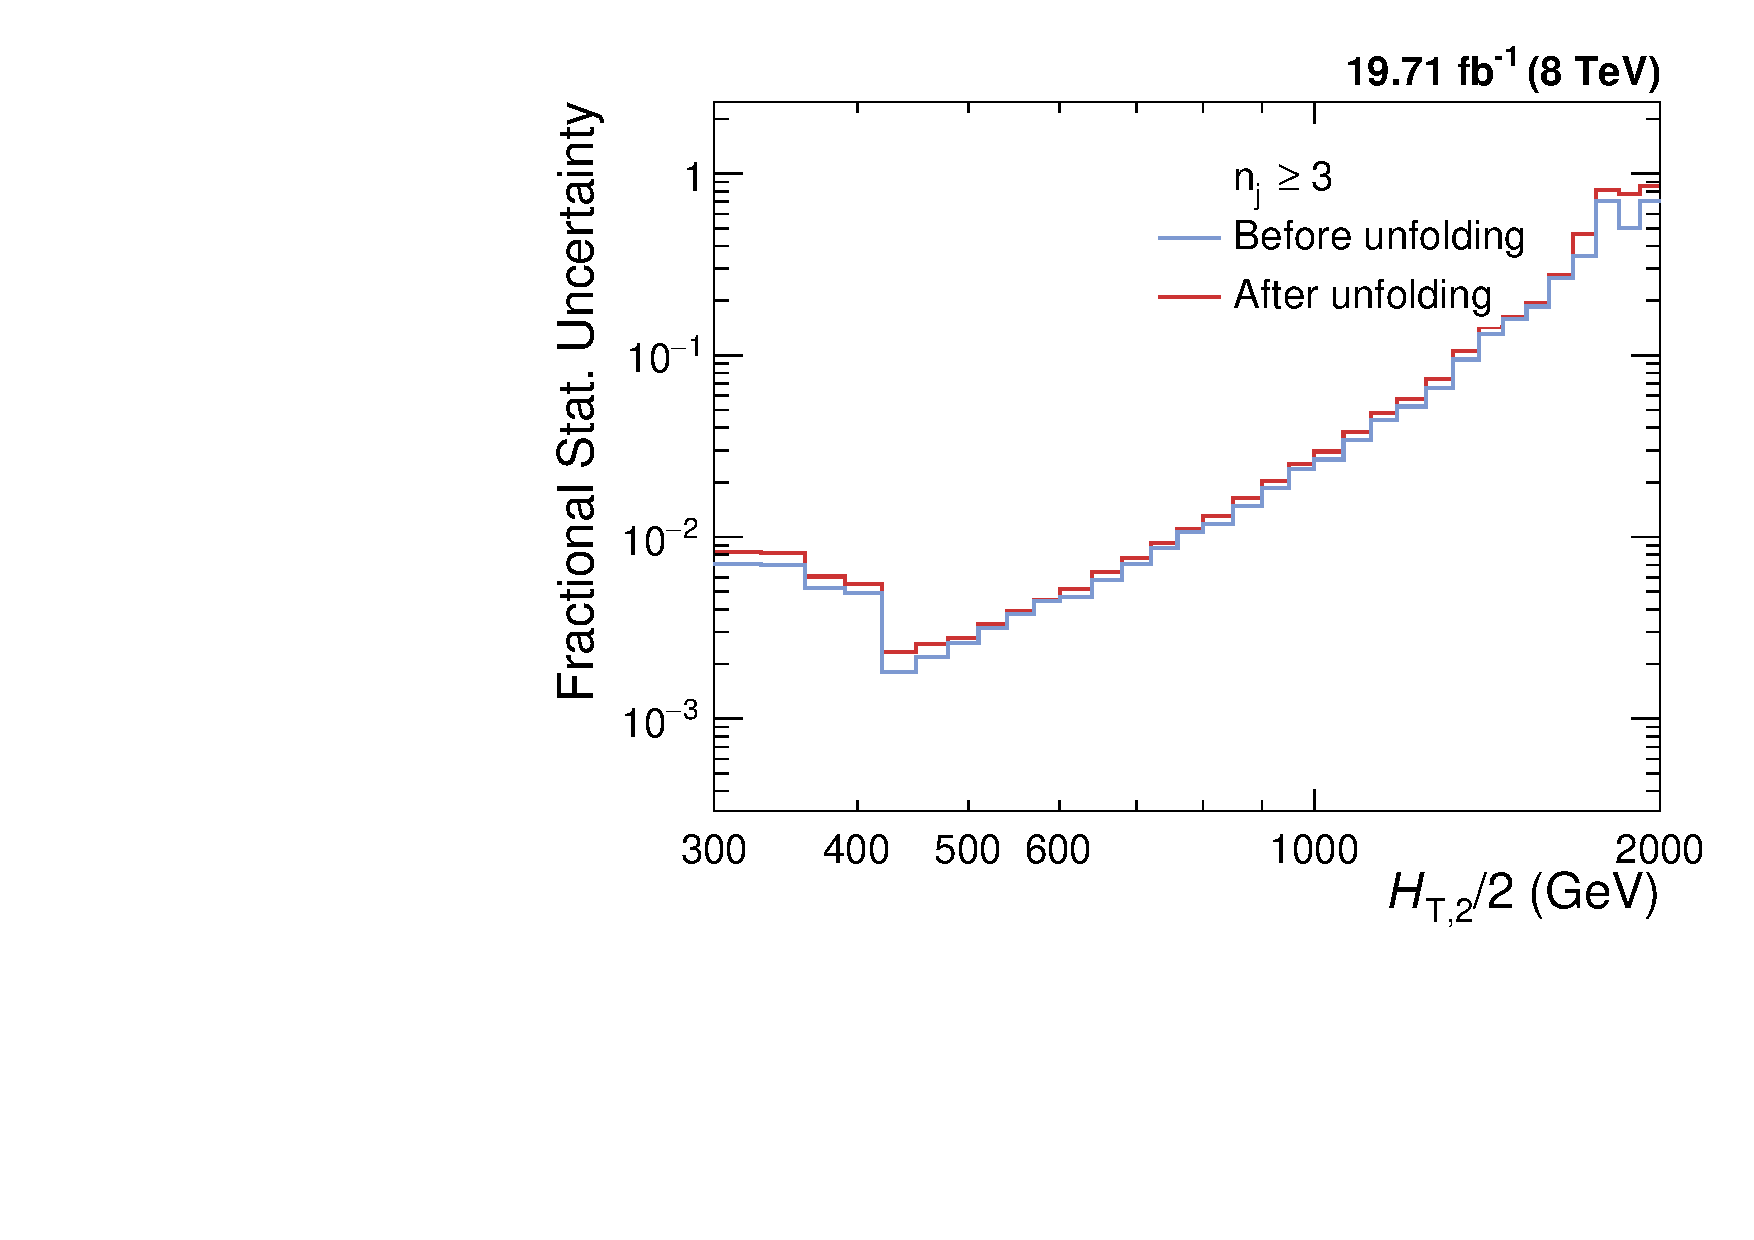
\includegraphics[width=0.51\textwidth]{Plots_HT_2_150/Comparison_stat_unc_3_HT_2_150.pdf}
 \caption{The fractional statistical uncertainties of the measured and the unfolded data for inclusive 2-jet events (left) and for inclusive 3-jet events (right). Depending on the unfolding procedure, the uncertainties can slightly increase, which is observed.}
 \label{fig:stat_unc}
 \end{center}
\end{figure}

Furthermore, the unfolding introduces a correlation between bins due to event migrations. These correlations are significant for neighbouring bins in \httwo and negligible between bins far off in the phase space. Figure~\ref{fig:corr} shows the correlations of the statistical uncertainty after the unfolding. We studied the correlations by performing unfolding with taking 4, 5 and 10 iterations and choosing the unfolding iteration parameter as ``4'' ensures that the statistical errors in the unfolded distributions are greater than that of the measured distributions. 

\begin{figure}[h]
 \begin{center}
 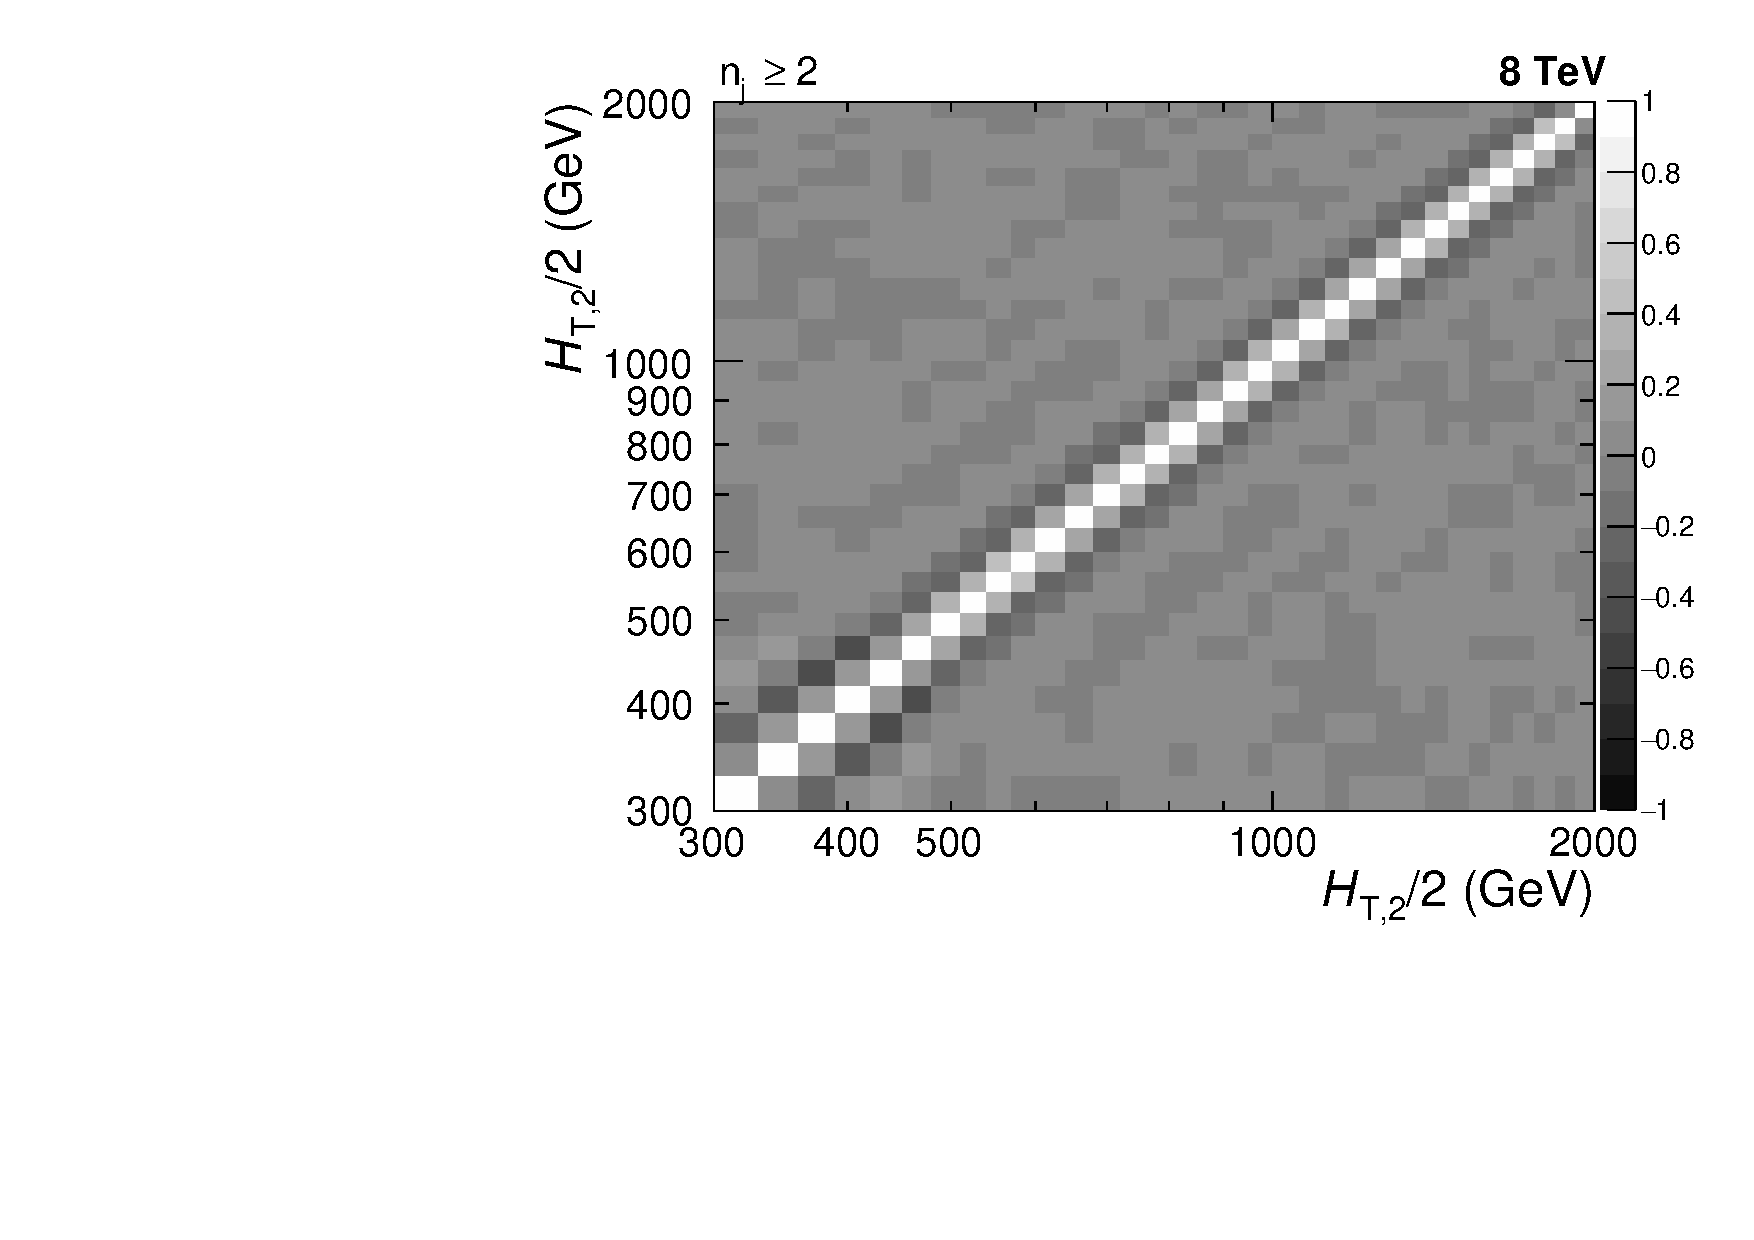
\includegraphics[width=0.51\textwidth]{Plots_HT_2_150/Correlation_Matrix_NLO_2_ite4.pdf}%
 ~~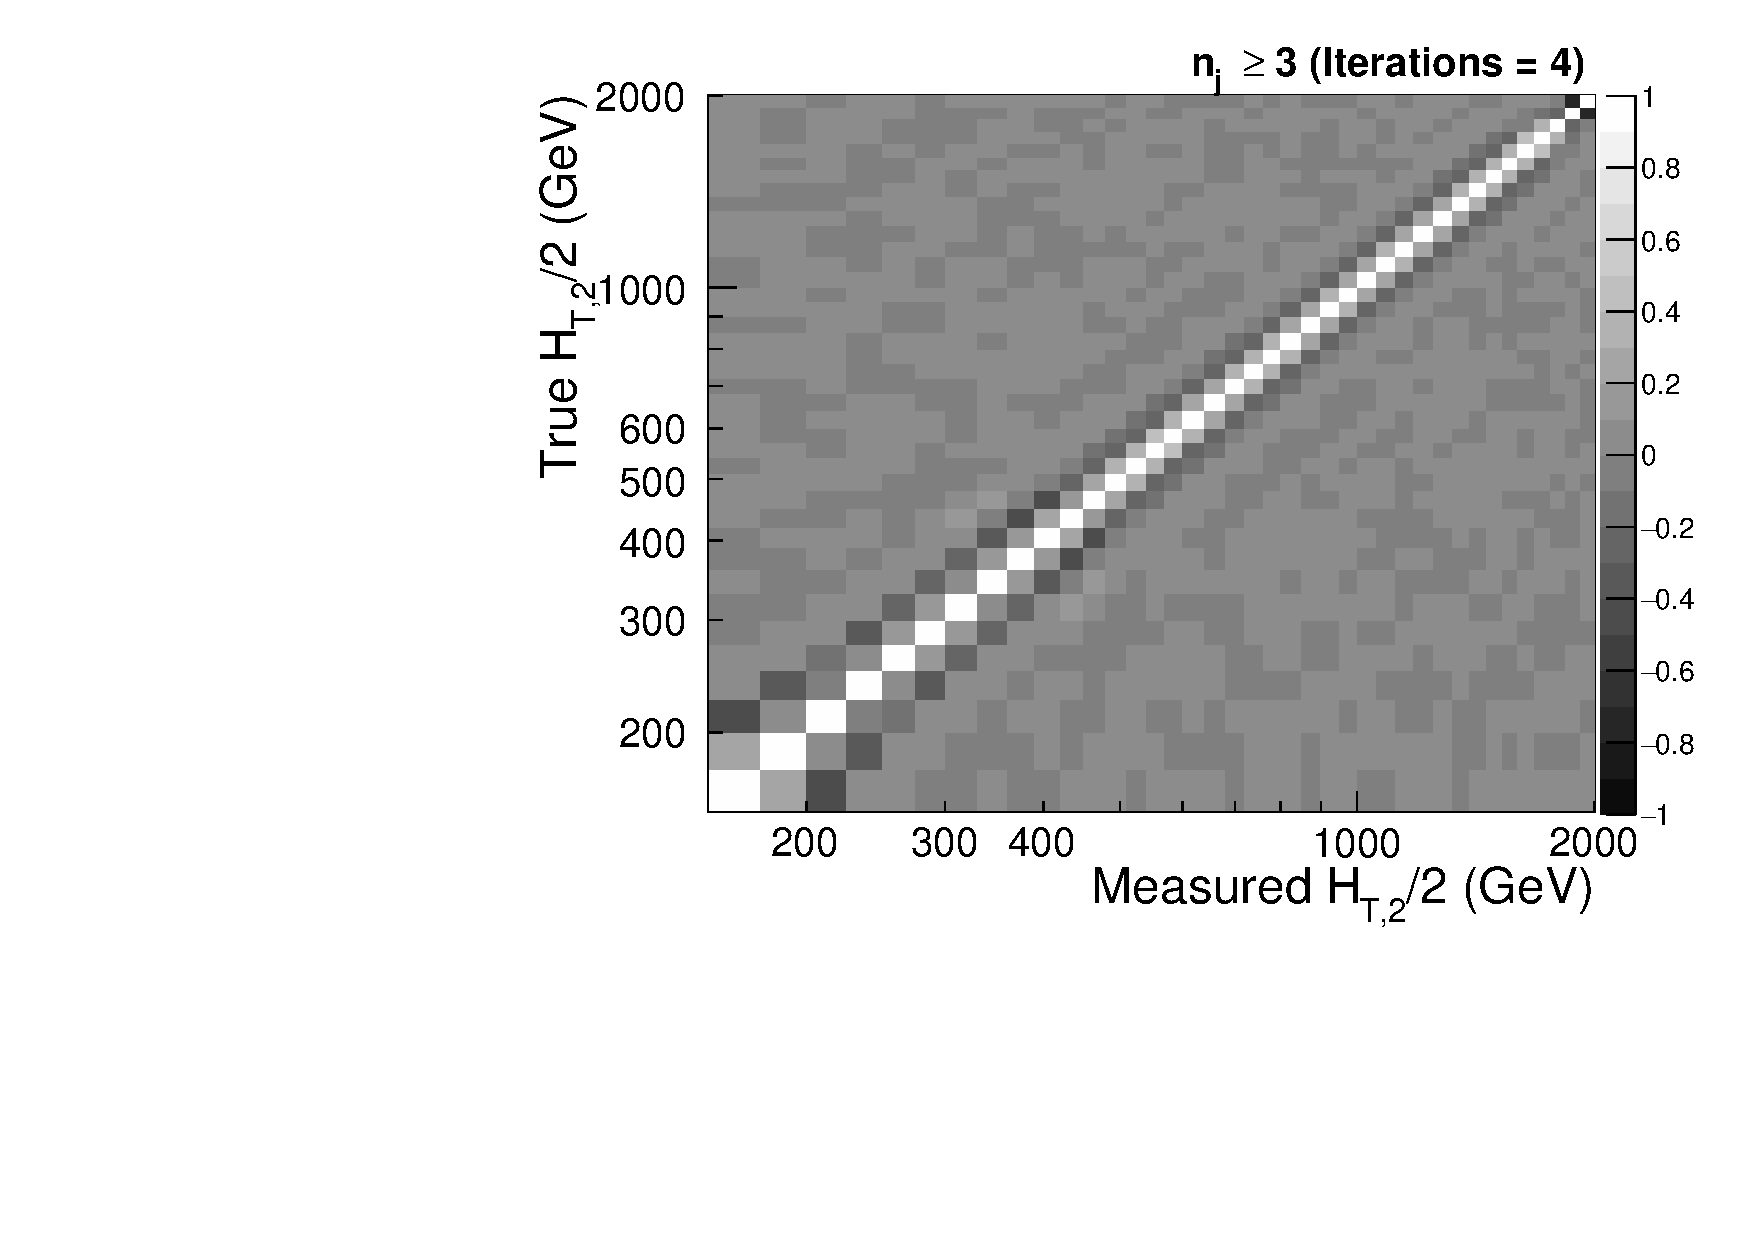
\includegraphics[width=0.51\textwidth]{Plots_HT_2_150/Correlation_Matrix_NLO_3_ite4.pdf}%
 \caption{Correlations of the statistical uncertainty introduced by the unfolding procedure for inclusive 2-jet events (Top) and for inclusive 3-jet events (Bottom) with 4 iterations (left), 5 iterations (middle) and 10 iterations (right). Neighbouring bins have a significant correlation or anti-correlation through bin migrations.}
 \label{fig:corr}
 \end{center}
\end{figure}

\subsection{Jet Energy Scale uncertainty}
The systematic uncertainty on the measured cross sections is asymmetric and dominated by the uncertainty on the jet-energy corrections (JEC). This is estimated by shifting the jet \pt according to the JEC uncertainty. The JEC uncertainties are split 
into 25 mutually independent sources of uncertainty, in which each source is fully correlated in \pt and $\eta$ but uncorrelated to all 
other sources and presents a 1$\sigma$ shift. \httwo is calculated by varying \pt and the difference from central \httwo gives JEC uncertainty as a function of \httwo. As these uncertainties can be asymmetric, the upwards and downwards variation of each source 
are treated separately. The sum in quadrature of all sources yields the total JEC uncertainty.

The sources of uncertainty are grouped in four categories according to their origin and details about the jet energy corrections and 
uncertainties are given %in~\cite{bib:JES_2013} and in : \\
https://twiki.cern.ch/twiki/bin/viewauth/CMS/ JECUncertaintySources\#Winter14\_uncertainties. 

The 25 individual uncertainty sources are the following :
AbsoluteStat, AbsoluteScale, AbsoluteFlavMap, AbsoluteMPFBias, Fragmentation, SinglePionECAL, 
SinglePionHCAL, FlavorQCD, RelativeJEREC1, RelativeJEREC2, RelativeJERHF,
RelativePtBB, RelativePtEC1, RelativePtEC2, RelativePtHF, RelativeFSR, RelativeStatFSR, RelativeStatEC2,
RelativeStatHF, PileUpDataMC, PileUpPtRef, PileUpPtBB, PileUpPtEC1, PileUpPtEC2 and PileUpPtHF.

The AbsoluteFlavMap uncertainty is exactly zero for the 8 TeV and can be ignored. In this way practically 24 uncertainties are considered to calculate JEC uncertainty. For the four sources : RelativeJERHF, 
RelativePtHF, RelativeStatHF, PileUpPtHF, the JEC uncertainty is exactly zero because of \abs{y} $<$ 2.5 cut used in the analysis. So only 20 sources contribute to the total JEC uncertainty. The Figures~\ref{fig:jes1}-\ref{fig:jes4} show the JEC uncertainty from each 
source separately for inclusive 2-jet (left) and 3-jet events (middle), respectively. The bin-wise values (in \%) are tabulated in the Tables~\ref{tab:exp_unc_jes_2},~\ref{tab:exp_unc_jes_2s} for inclusive 2-jet and~\ref{tab:exp_unc_jes_3},~\ref{tab:exp_unc_jes_3s} for inclusive 3-jet events. 
\end{comment}
\subsection{Unfolding uncertainty}
\label{sec:unfolding_unc}

The unfolding uncertainty is comprised of three uncertainties :

\begin{enumerate}
\item {\bf JER uncertainty :} The jet energy resolution, which was derived in Section~\ref{subsec:Resolution}, is used to produce the response matrix using a forward 
smearing technique in the unfolding procedure. Therefore, a dependence on the jet energy resolution on the unfolded cross section is 
introduced and a further uncertainty source due to the uncertainty on the jet energy resolution is introduced. Table~\ref{resolution} shows 
the scaling factors, which were applied on reconstructed simulated events to obtain the actual resolution in data. The official 
recommendations include offset variations of these scaling factors to estimate the uncertainty on the resolution and are also given in Table~\ref{resolution}. The 
determination of the resolution is repeated with the upwards and downwards variation of the resolution scaling factor applied. The 
unfolding procedure is also reiterated using the variations of the resolution and the differences of the obtained cross section to the 
nominal cross section are accounted for as a systematic uncertainty. 

\item {\bf Model dependence :} As explained earlier that to construct the response matrix by Toy MC method, the fitting of the theoretical predictions is performed by using function given in Equation~\ref{eq:func1}. To use alternative function for this fitting gives the model dependence of the theoretical \httwo spectrum which affects the response matrix and thus the unfolding.
The NLO \httwo spectrum is fitted by the another function described by Equation~\ref{eq:func2}. The procedure mentioned in Section~\ref
{sec:unfolding} is repeated to get the new unfolded cross sections. The differences in unfolded cross sections using the functions given by equations~
\ref{eq:func1} and~\ref{eq:func2} gives the unfolding uncertainty. 

\item {\bf Additional uncertainty :} As explained in Section~\ref{subsec:Resolution}, an additional uncertainty is added from the difference in unfolding on comparing with reduced JER.

\end{enumerate}

All the three uncertainties are added in quadrature to account the unfolding uncertainty which is 1-2\% on cross-sections.

While calculating JER where one large rapidity bin is used, it has been observed that from Figure~\ref{fig:ratios}, when JER extracted from \textcolor{blue}{simulated MG\plus P6 Reco/MG\plus P6 Gen} is used in toyMC for smearing, it smears the fastNLO too much (\textcolor{mycolor}{red curve}). The extracted JER also smears MC Gen more as seen from Smeared MG\plus P6 Gen/MG\plus P6 Gen (black dashed curve). When the 30\% reduced JER  is used to smear MG\plus Gen, the \textcolor{pink}{Smeared MG\plus Gen/MG\plus P6 Gen}, matches with simulated \textcolor{blue}{MG\plus P6 Reco/MG\plus P6 Gen}. Also, toyMC Gen smeared with 30\% reduced  JER, \textcolor{green}{Smeared FastNLO/Gen FastNLO}. So an additional unfolding uncertainty is attributed by comparison to 30\% reduced JER.  

\begin{figure}[!htbp]
  \begin{center}
    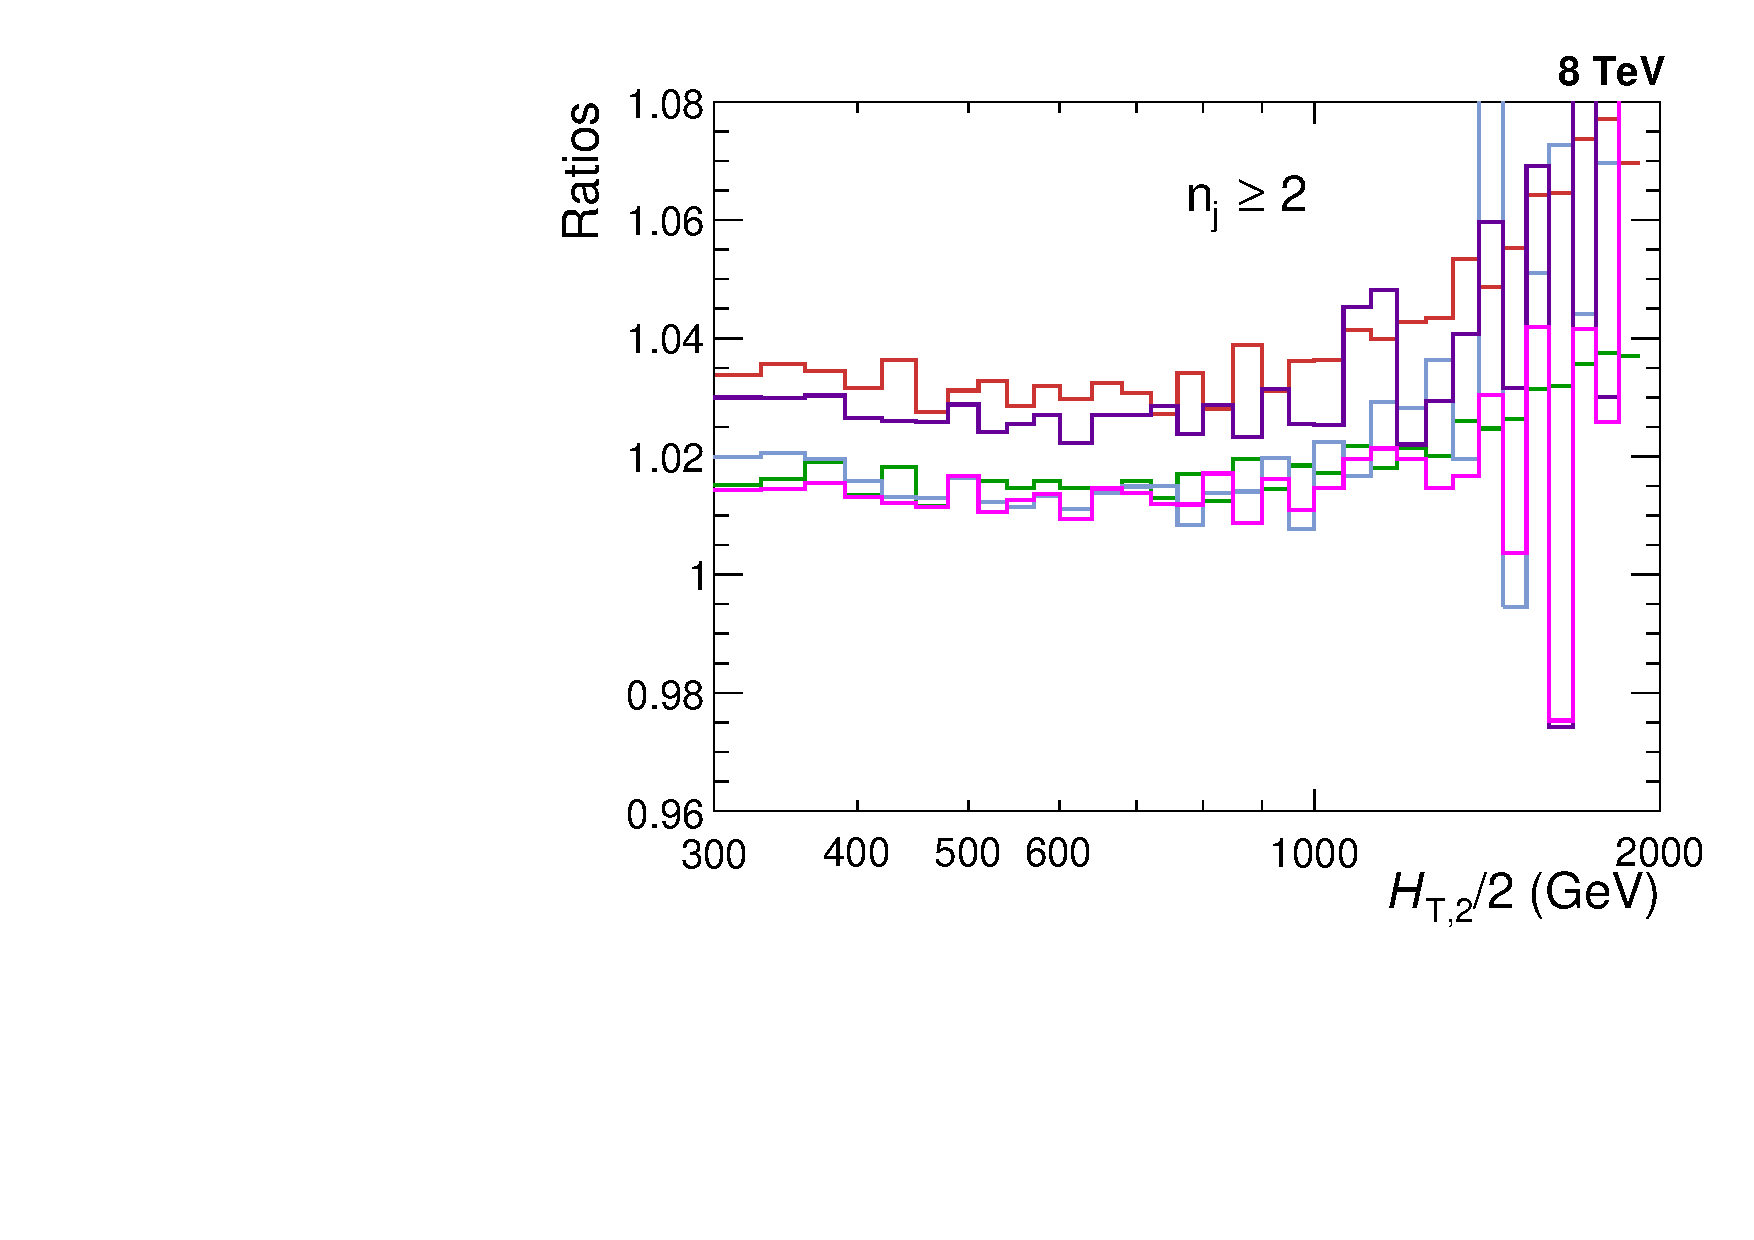
\includegraphics[width=0.51\textwidth]{Plots_HT_2_150/Ratio_all_2_crystal.pdf}%
    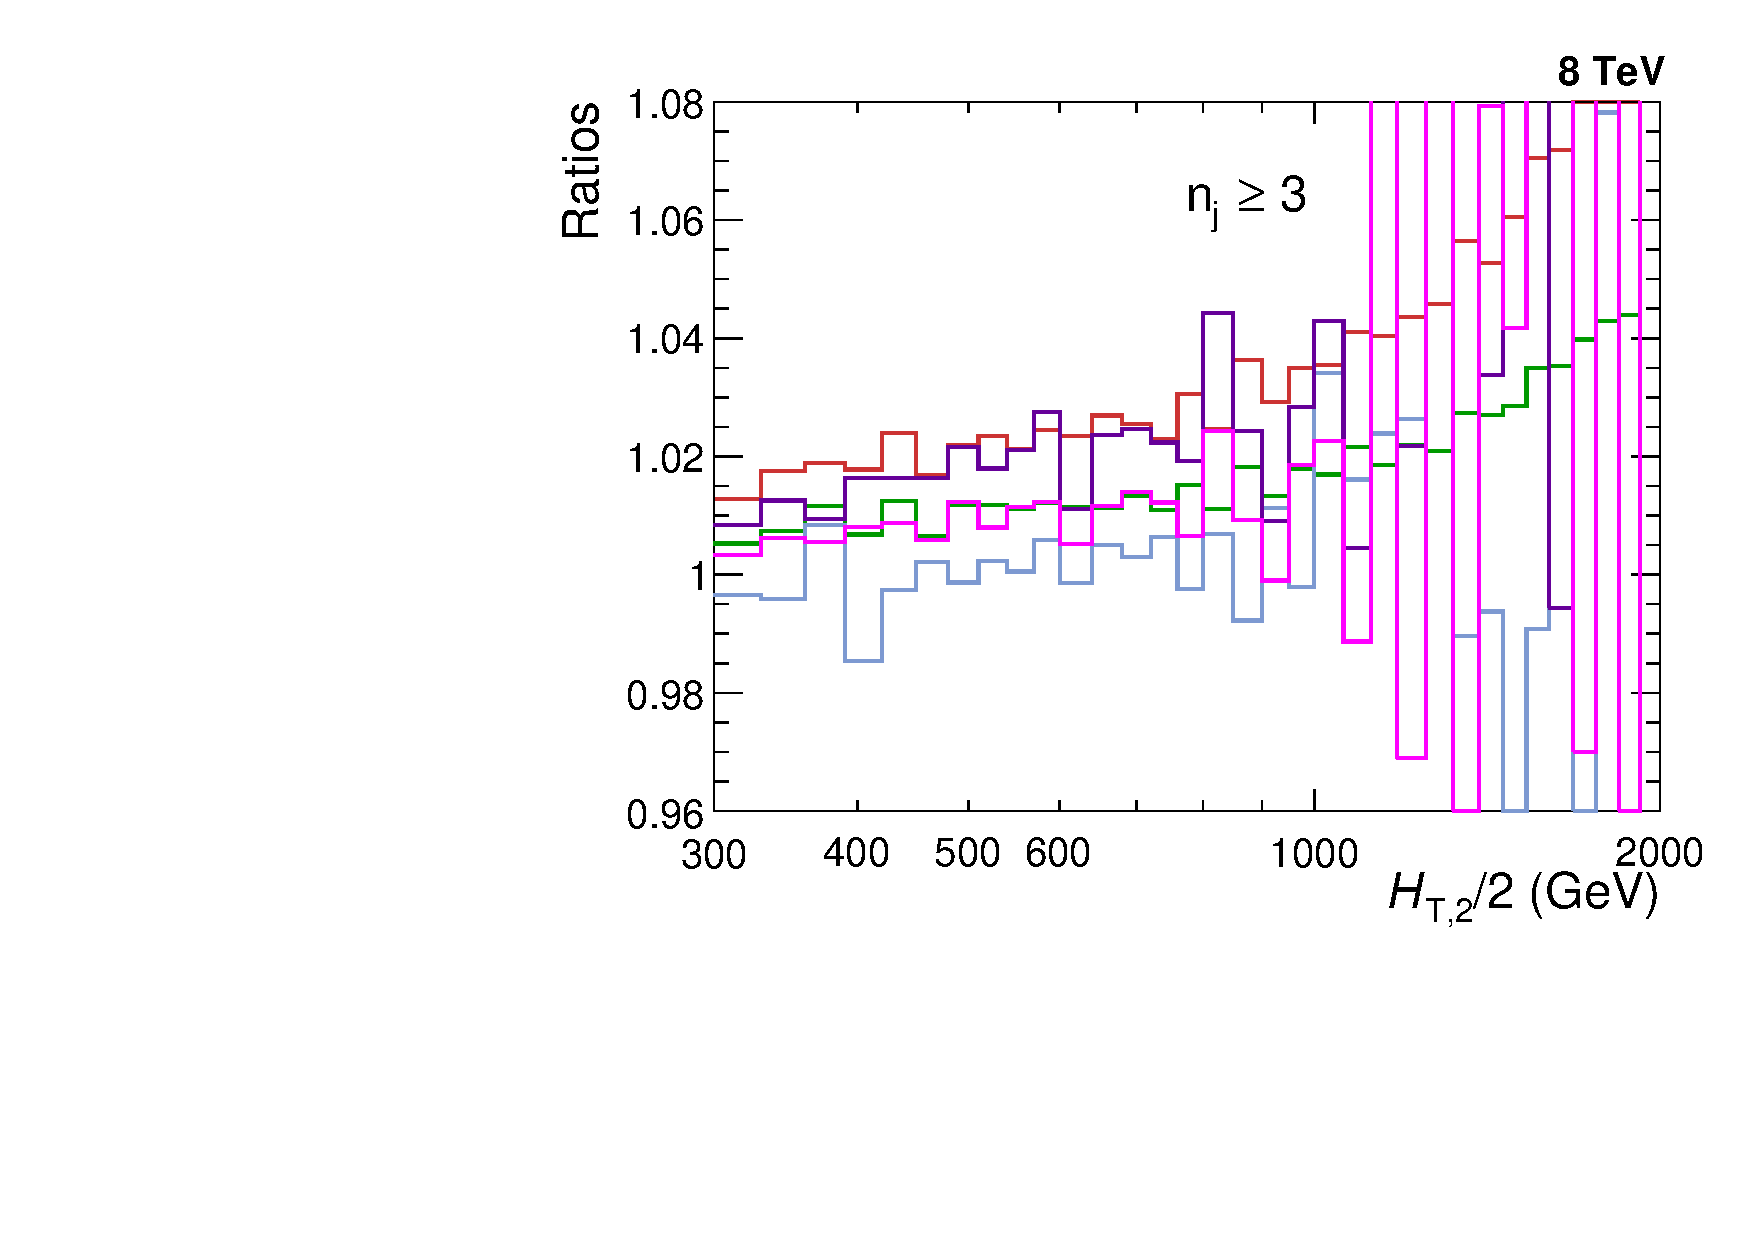
\includegraphics[width=0.51\textwidth]{Plots_HT_2_150/Ratio_all_3_crystal.pdf}\\
    \caption{\textcolor{blue}{Simulated MG\plus P6 Reco/MG\plus P6 Gen} to extract JER, \textcolor{red}{Smeared FastNLO/Gen FastNLO} using extracted JER, Smeared MG\plus P6 Gen/MG\plus P6 Gen using extracted JER, \textcolor{pink} {smeared MG\plus P6 Gen/MG\plus P6 Gen} using 30\% reduced extracted JER, \textcolor{green}{Smeared FastNLO/Gen FastNLO} using 30\% reduced extracted JER; for inclusive 2-jet (left) and inclusive 3-jet events (right).}
    }\label{fig:ratios}
  \end{center}
\end{figure}

\subsection{Total experimental uncertainty}
After calculating the uncertainties from all different sources, total experimental uncertainty is obtained by adding in quadrature the 
uncertainties from individual sources. The bin-wise values (in \%) of uncertainties from each source as well as total uncertainty are tabulated in Table~\ref{tab:exp_unc2} and Table~\ref{tab:exp_unc3} for inclusive 2-jet and inclusive 3-jet events, respectively. Figure~\ref{fig:exp_unc} show the uncertainties from all sources of 
experimental uncertainty as well as the total uncertainty for inclusive 2-jet (left) and inclusive 3-jet (right) events. The systematic uncertainty on the measured cross 
sections is asymmetric and dominated by the uncertainty on the jet-energy scale at lower \httwo values and by statistical uncertainty at 
higher \httwo values. The experimental uncertainties from each source as well as total uncertainty are quoted in Table~\ref{tab:exp_unc_overview}. 

\begin{figure}[!htbp]
 \begin{center}
 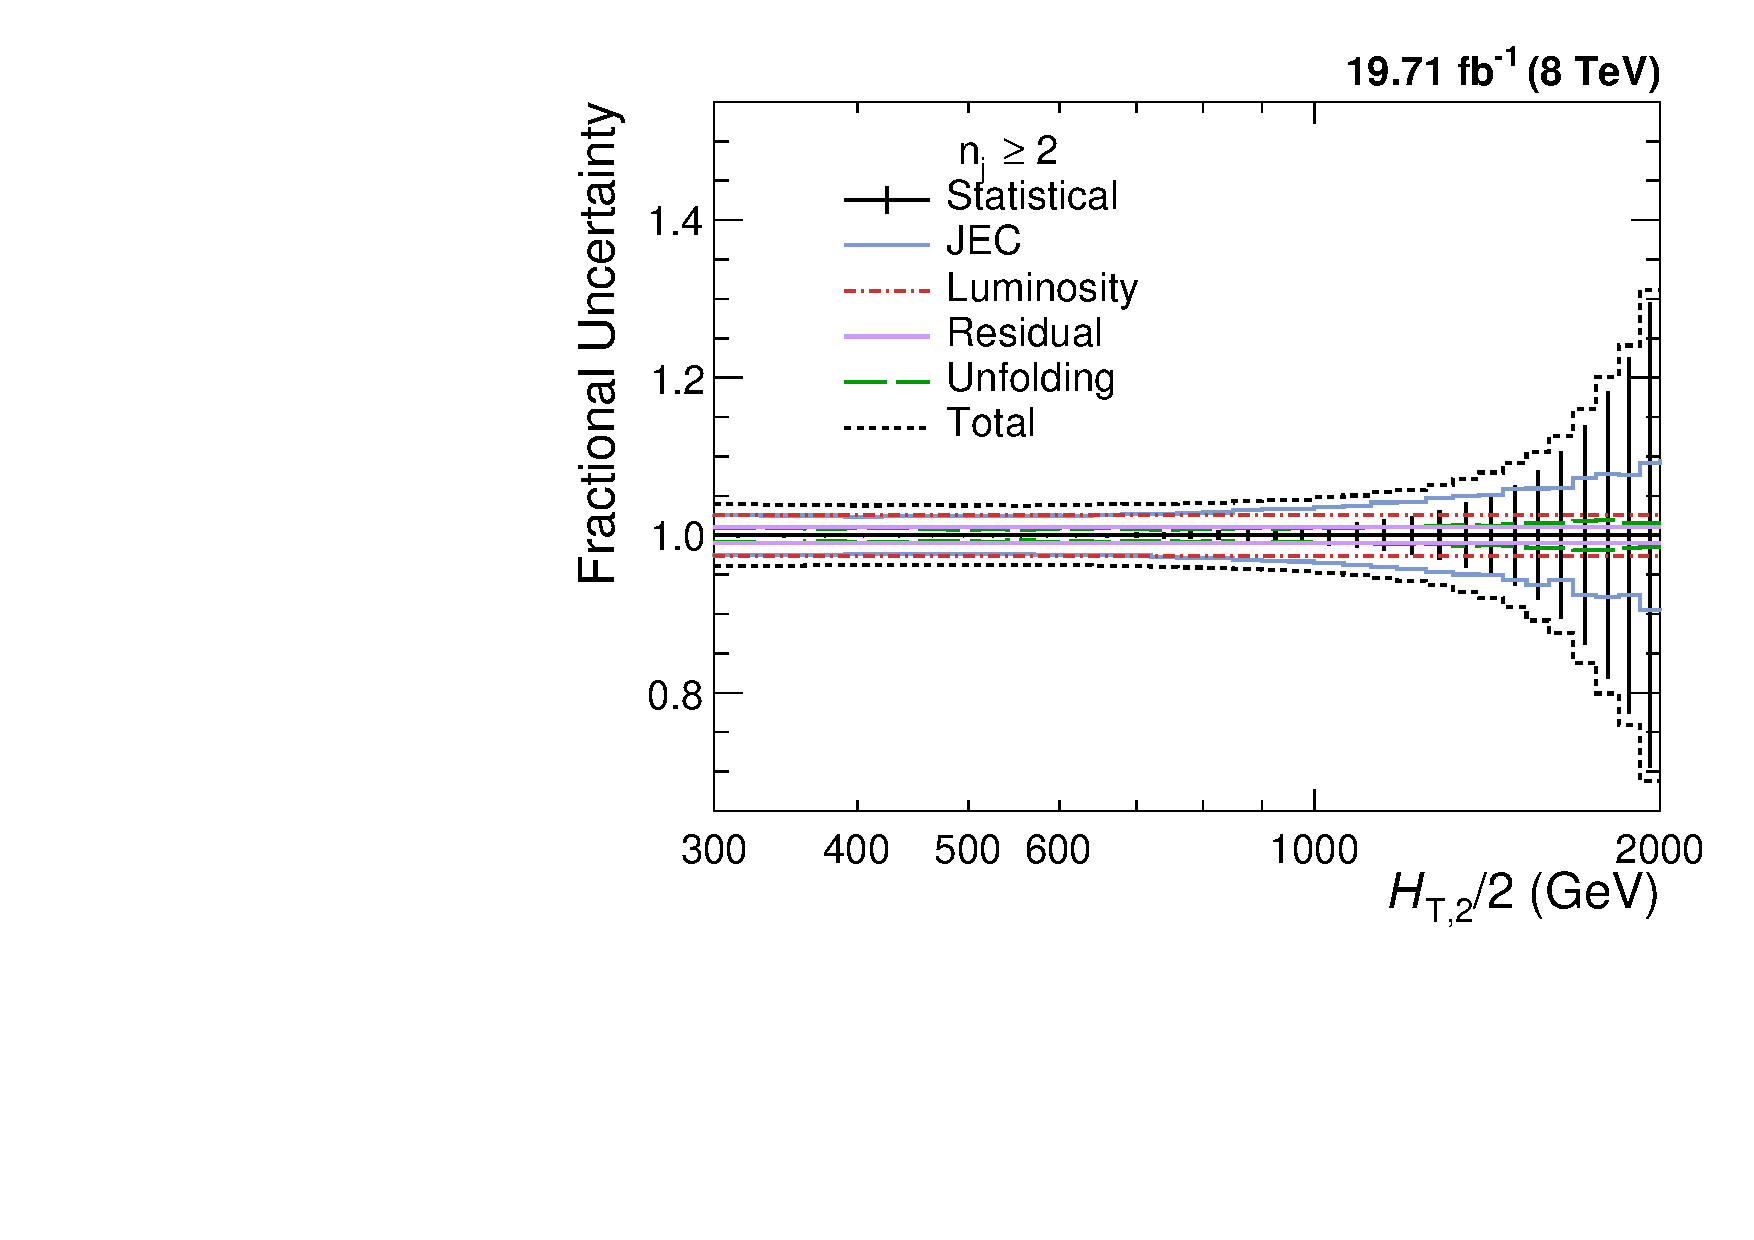
\includegraphics[width=0.51\textwidth]{Plots_HT_2_150/Total_unc_all_2_NLO_add.pdf}%
 ~~\includegraphics[width=0.51\textwidth]{Plots_HT_2_150/Total_unc_all_3_NLO_add.pdf}
 \caption{Overview of all experimental uncertainties affecting the cross section measurement for inclusive 2-jet (left) and inclusive 3-jet (right). The error bars indicate the statistical uncertainty after unfolding. The colored lines give the uncertainties resulting of jet energy scale, luminosity, unfolding and residual effects. The total uncertainty is calculated by adding in quadrature the individual sources of uncertainty.}
 \label{fig:exp_unc}
 \end{center}
\end{figure}

\begin{table}[!htbp]
\caption{Overview of all experimental uncertainties affecting the cross section measurement.}
\label{tab:exp_unc_overview}
  \centering
  \begin{tabular}{ccc}
    \hline\hline
     Uncertainty Source & {\bf Inclusive 2-jet} & {\bf Inclusive 3-jet} \rbthm\\\hline     
     {\bf Statistical}  & $<$ 1 to 30\% & $<$ 1 to 40\% \rbtrr\\
     {\bf \blue {JEC}}  & 3 to 10\% & 4 to 12\% \rbtrr\\
     {\bf \textcolor{green!50!black} {Unfolding}} & 1-2\% & 1-2\% \rbtrr\\
     {\bf \mycolor {Luminosity}} & 2.6\% & 2.6\% \rbtrr\\
     {\bf \textcolor{red!30!blue!50!white} {Residual uncorrelated}} & 1\% & 1\% \rbtrr\\
  \hline\hline
  \end{tabular}
\end{table}
\begin{comment}
\section{Measurement of cross section ratio, unfolding and experimental uncertainties}
\subsection{Measurement of cross section ratio}
The ratio of cross sections, $R_{mn}$ as a function of $\httwo$, is extracted by dividing the cross section of selected inclusive m-jet 
events to that of inclusive n-jet events at any given bin size of \httwo. The ratios \ratio, $R_{43}$ and $R_{42}$ are calculated. In cross 
section ratios, the numerator and denominator are not independent samples. So to calculate the statistical uncertainty for the cross 
section ratios before unfolding, the Wilson score interval is used which takes into account the correlation between the numerator and the denominator and 
give asymmetric errors. For example, the bin-wise inclusive 2-jet and 3-jet differential cross sections as well as cross section ratio \ratio, calculated at detector level, along with statistical uncertainty (in \%) are tabulated in Table~\ref{tab:ratio_32}. 

Figure~\ref {fig:ratio_32} shows the ratio $R_{mn}$ as a function of $\httwo$ : \ratio data (black solid circles), \ratio~\MadGraphF + \PYTHIAS MC 
(red solid circles) and \ratio NLO (green solid line), $R_{43}$ data (black solid triangles (up)), $R_{43}$ \MadGraphF + \PYTHIAS MC (red 
solid triangles (up)) and $R_{42}$ data (black solid triangles (down)), $R_{42}$ \MadGraphF + \PYTHIAS MC (red solid triangles (down)). The 
ratios $R_{mn}$ from data are in well agreement with that from MC as well as NLO predictions.

\begin{figure}[!htbp]
  \begin{center}
    \includegraphics[width=0.5\textwidth]{Plots_HT_2_150/Ratio_32_43_42_all_HT_2_150.pdf}
    \caption{Cross section ratios $R_{mn}$ as a function of $\httwo$. The error bars give the statistical uncertainty, calculated by the Wilson score interval which takes into the account the correlation between the numerator and the denominator.}
    \label{fig:ratio_32}
  \end{center}
\end{figure}

\subsection{Unfolding}
The measured ratio \ratio as a function of \httwo, is then corrected for detector smearing effects and unfolded to particle level. There can be two ways to obtain  unfolded cross section ratio :

\begin{enumerate}
\item To unfold separately the inclusive 2-jet and 3-jet measured cross sections and then construct the ratio \ratio 
\item To unfold directly the ratio \ratio
\end{enumerate}

%Both methods gave the same results. 
In the first method, we have ratios of unfolded cross sections by using response matrices constructed using Toy MC method i.e. smeared NLO matrices (Figure~\ref{fig:response_NLO}) as well as by using response matrices from \MadGraphF + \PYTHIAS MC (Figure~\ref{fig:response_MC}). Figure~\ref{fig:ratio_unfolded_32} left shows the comparison of \ratio, obtained from data unfolded using smeared NLO matrix (black solid circles) and the one unfolded using MC matrix (red solid circles), with \ratio from NLO prediction (red line). As the matrices from MC are also available for inclusive 4-jet events, so these can used to unfold the ratios $R_{43}$ and $R_{42}$ as shown in Figure~\ref{fig:ratio_unfolded_32} with black solid triangles (up) and black solid triangles (down), respectively.

In further analysis, cross section ratio obtained from data, unfolded using smeared NLO matrix is considered. Since the theory NLO predictions are available for inclusive 2-jet and 3-jet events and not for inclusive 4-jet events yet, so only ratio \ratio is used in further analysis. Figure~\ref{fig:ratio_unfolded_32} right gives the ratio of unfolded \ratio calculated from ratio of unfolded cross sections to that of measured one using central JER (black solid circles) as well as reduced JER (green solid circles).  We have used first method to calculate the systematic uncertainties.

 \begin{figure}[!htbp]
  \begin{center}
    \includegraphics[width=0.5\textwidth]{Plots_HT_2_150/Ratio_32_43_42_unfolded_all_HT_2_150.pdf}%
    \includegraphics[width=0.5\textwidth]{Plots_HT_2_150/Ratio_Unfolding_data_NLO_ratio32.pdf}\\
    \caption{Left figure shows the unfolded \ratio,  obtained from data unfolded using smeared NLO matrix (black solid circles), from data unfolded using MC matrix (red 
    solid circles) and from NLO prediction (red line); $R_{43}$ from the data unfolded using MC matrix (black solid triangles (up)) and $R_
    {42}$ from data unfolded using MC matrix (black solid triangles (down)). Right gives the ratio of unfolded \ratio calculated from ratio of unfolded cross sections to that of measured one using central JER (black solid circles) as well as reduced JER (green solid circles).}
    \label{fig:ratio_unfolded_32}
  \end{center}
\end{figure}

\subsubsection{Response matrix}
To unfold directly the ratio \ratio, we need to construct the response matrix using Toy MC method as explained in section~\ref
{sec:unfolding}. To obtain the true spectrum for \ratio, the ratio of theory predictions, extrapolated with function I (equation~\ref
{eq:func1}, for inclusive 3-jet to that of 2-jet is taken, as shown in Figure~\ref{fig:fit} (Top). Then this ratio is fitted using the polynomial function of degree 8 as shown in Figure~\ref{fig:ratio_fit}.
 
 \begin{figure}[!htbp]
  \begin{center}
    \includegraphics[width=0.6\textwidth]{Plots_HT_2_150/Extrapolate_Theory_Ratio_32.pdf}
    \caption{Fitted NLO spectrum of cross section ratio \ratio as a function of \httwo using polynomial function of degree 8.}
    \label{fig:ratio_fit}
  \end{center}
\end{figure}

A flat \httwo spectrum is generated and the fit parameters obtained from polynomial fit provides weights to the flat spectrum. A total of 
ten million events are generated (in \httwo range 80-2000). These generated values are smeared with a Gaussian function, where $\sigma$ of 
the Gaussian is determined from the relative resolution parametrization as a function of \httwo calculated from NSC formula mentioned in 
equation~\ref{NSC_formula}. The parameters N, S, C used for smearing are taken to be same for inclusive 3-jet events, as mentioned in Table~\ref{fit_para}.

These generated and smeared values are used to fill the response matrices by using the RooUnfold package. Figure~\ref
{fig:unfolded_ratio} (left) shows the response matrix derived using the Toy MC for ratio \ratio. The matrix is normalized to the number of 
events in each column. The response matrix is diagonal with small off-diagonal migrations between close-by \httwo bins.

First we unfold the smeared spectrum obtained from Toy MC to perform the closure test. Figure~\ref{fig:unfolded_ratio} (right) shows 
that after unfolding, the smeared spectrum matches exactly with the randomly generated spectrum as expected. The bottom plot gives the ratio of unfolded 
%ratio calculated from the unfolded cross sections to that of the measured one. The unfolding works well above 300 GeV and considering the the lack of statistical precision beyond 1680 GeV for inclusive 3-jet events (from Table~\ref{tab:ratio_32}), the ratio distributions are plotted in the range 300-1680 GeV. 
%Then the measured ratio \ratio 
%from data is unfolded using the above reconstructed response matrix. The unfolded \ratio is compared to that of measured (bottom left) 
%in Figure~\ref{fig:unfolded_ratio}. As explained earlier, the Wilson score interval method to calculate the statistical uncertainty on the 
%measured ratio, gives the asymmetric statistical errors. So the measured ratio is unfolded two times : once with Up and and then with Low 
%statistical errors to get the asymmetric statistical uncertainties after unfolding. The right hand side plot gives the ratio of unfolded 
%ratio calculated from the unfolded cross sections to that of the measured one. The unfolding works well above 300 GeV and considering the the lack of statistical precision beyond 1680 GeV for inclusive 3-jet events (from Table~\ref{tab:ratio_32}), the ratio distributions are plotted in the range 300-1680 GeV.
\begin{figure}[!htbp]
  \begin{center}
    \includegraphics[width=0.45\textwidth]{Plots_HT_2_150/Normalized_Response_Matrix_NLO_ratio_32_column_2.pdf}
    \includegraphics[width=0.45\textwidth]{Plots_HT_2_150/Ratio_Unfolding_NLO_Ratio_32_ToyMC.pdf}\\
    %\includegraphics[width=0.45\textwidth]{Plots_HT_2_150/Ratio_Unfold_data_ratio_32_direct_ToyMC.pdf}
    %\includegraphics[width=0.45\textwidth]{Plots_HT_2_150/Ratio_Unfold_data_ratio_32_unfoldedx.pdf}
    \caption{The response matrix derived using the Toy MC for ratio \ratio (left) and Closure test (right).}% and ratio of unfolded direct \ratio to that of measured (bottom left), with statistical uncertainties Up (solid line) as well as statistical uncertainties Low (dashed line),     The ratio of unfolded \ratio calculated from ratio of unfolded cross sections to that of measured one (bottom).}
    \label{fig:unfolded_ratio}
  \end{center}
\end{figure}

\subsection{Experimental uncertainties}
In cross section ratio, the uncorrelated and luminosity uncertainties got cancel. The experimental sources of uncertainty which affect the cross section ratio measurement includes - 

\begin{itemize}
\item the statistical uncertainty : propagated through the unfolding, 
\item the jet energy correction uncertainty (JEC) : uncertainty due to the calibration of the jet energy, 
\item the unfolding uncertainty : unfolding procedure.
\end{itemize}

\subsubsection{Statistical uncertainty}
\label{sec:unfolding_stat_ratio}
The statistical uncertainties for ratio \ratio are calculated in the same way as it was done for inclusive 2-jet and 3-jet cross sections, explained in section~\ref{sec:unfolding_stat}. Figure~\ref{fig:stat_unc_ratio} shows the relative statistical uncertainty before and after the unfolding procedure. 

\begin{figure}[!htbp]
  \begin{center}
    \includegraphics[width=0.5\textwidth]{Plots_HT_2_150/Comparison_stat_unc_ratio_32_up.pdf}%
    \includegraphics[width=0.5\textwidth]{Plots_HT_2_150/Comparison_stat_unc_ratio_32_down.pdf}\\
    \caption{The fractional statistical uncertainties Up (left) and Low (right), of the unfolded as well as measured cross section ratio \ratio. Depending on the unfolding procedure, the uncertainties can slightly increase, which is observed.}
    \label{fig:stat_unc_ratio}
  \end{center}
\end{figure}

The uncertainty slightly increases during the unfolding process. Also, the unfolding introduces a correlation between bins due to
event migrations. To find the correlations of the statistical uncertainty introduced by the unfolding procedure for ratio, \ratio, firstly 
ratio is calculated and then unfolded this ratio to particle level. Figure~\ref{fig:corr_ratio} shows the correlations of the statistical 
uncertainty after the unfolding. We studied the correlations by performing unfolding with taking 4, 5 and 10 iterations and choosing the 
unfolding iteration parameter as ``4'' ensures that the statistical errors in the unfolded distributions are greater than that of the 
measured distributions. 

\begin{figure}[!htbp]
  \begin{center}
    \includegraphics[width=0.35\textwidth]{Plots_HT_2_150/Correlation_Matrix_NLO_Ratio_32_ite4.pdf}%
    \includegraphics[width=0.35\textwidth]{Plots_HT_2_150/Correlation_Matrix_NLO_Ratio_32_ite5.pdf}%
    \includegraphics[width=0.35\textwidth]{Plots_HT_2_150/Correlation_Matrix_NLO_Ratio_32_ite10.pdf}\\
    \caption{Correlations of the statistical uncertainty introduced by the unfolding procedure for ratio \ratio with 4 iterations (left), 5 iterations (middle) and 10 iterations (right). Neighbouring bins have a significant correlation or anti-correlation through bin migrations.}
    \label{fig:corr_ratio}
  \end{center}
\end{figure}

\subsubsection{Jet Energy Scale uncertainty}
The systematic uncertainty on the measured cross sections is asymmetric and dominated by the uncertainty on the jet-energy correction (JEC) at low \httwo. To calculate JEC uncertainty for ratio \ratio, the inclusive 2-jet and 3-jet events cross sections are measured as a function of \httwo by shifting the jet \pt according to the JEC uncertainty for each source separately. Then the ratio of these cross sections, \ratio is taken and the difference from the central ratio \ratio, gives the JEC uncertainty for each source. As these uncertainties can be asymmetric, the upwards and downwards variation of each source are treated separately. The sum in quadrature of all sources yields the total JEC uncertainty.

The Figures~\ref{fig:jes1}-\ref{fig:jes4} show the JEC uncertainty from each source separately for ratio \ratio (right). As expected, the JEC uncertainty for ratio is less than that for inclusive cross sections. The bin-wise values (in \%) are tabulated in the Tables~\ref{tab:exp_unc_jes_r} and ~\ref{tab:exp_unc_jes_rs}.

\subsubsection{Unfolding uncertainty}
\label{sec:unfolding_unc_ratio}
As explained earlier in section~\ref{sec:unfolding_unc}, the three uncertainties are considered for \ratio :

\begin{enumerate}
\item {\bf JER uncertainty :} To determine JER uncertainty, ratio \ratio is calculated from the cross sections as a function of \httwo measured with the upwards and downwards variation of the resolution scaling factor as described in section~\ref{sec:unfolding_unc}. The differences of the obtained cross section ratio to the nominal cross section ratio are accounted as a systematic uncertainty. 

\item {\bf Model dependence : } As explained earlier in section~\ref{sec:unfolding_unc}, the differences in cross section ratios obtained from unfolded cross sections using the functions given by equations~\ref{eq:func1} and~\ref{eq:func2} gives the unfolding uncertainty. 

\item {\bf Additional uncertainty : } The additional uncertainty resulting from differences in unfolded cross-sections with central JER and 30\% reduced JER is added.

\end{enumerate}

All the three uncertainties are added to the unfolding uncertainty which is 1\% for \ratio.

\subsubsection{Total experimental uncertainty}
After calculating the uncertainties from all different sources, total experimental uncertainty is obtained by adding in quadrature the 
uncertainties from individual sources. The bin-wise values (in \%) of uncertainties from each source as well as total uncertainty are tabulated in Table~\ref{tab:exp_unc_ratio}. Figure~\ref{fig:exp_unc_ratio} show the uncertainties from all sources of 
experimental uncertainty as well as the total uncertainty. The systematic uncertainty on the measured cross 
sections is asymmetric and dominated by the uncertainty on the jet-energy scale at lower \httwo values and by statistical uncertainty at 
higher \httwo values. The experimental uncertainties from each source as well as total uncertainty are quoted in Table~\ref{tab:exp_unc_overview}.

\begin{figure}[!htbp]
  \begin{center}
    \includegraphics[width=0.5\textwidth]{Plots_HT_2_150/Total_Unc_ratio_32_direct_add.pdf}
    \caption{Overview of all experimental uncertainties affecting the cross section \ratio as a function of \httwo. The error bars indicate the statistical uncertainty. The colored lines give the uncertainties resulting of jet energy scale and unfolding. The total uncertainty is calculated by adding in quadrature the individual sources of uncertainty.}
    \label{fig:exp_unc_ratio}
  \end{center}
\end{figure}

\begin{table}[!htbp]
\caption{Overview of all experimental uncertainties affecting the cross section ratio, \ratio.}
\label{tab:exp_unc_ratio_overview}
  \centering
  \begin{tabular}{cc}
    \hline\hline
     Uncertainty Source & {\bf Ratio \ratio}  \rbthm\\\hline
     {\bf Statistical}  & $<$ 1 to $>$ 50\%  \rbtrr\\
     {\bf \blue {JEC}}  & 1 to 2\% \rbtrr\\
     {\bf \textcolor{green!50!black} {Unfolding}} & 1\%  \rbtrr\\
     {\bf \mycolor {Luminosity}} & cancels \rbtrr\\
     {\bf \textcolor{red!30!blue!50!white} {Residual uncorrelated}} & cancels \rbtrr\\
  \hline\hline
  \end{tabular}
\end{table}

\section{Theory predictions}
\label{sec:theory predictions}
\subsection{Fixed order NLO calculations}
Predictions at NLO accuracy in pQCD are computed with the \NLOJETPP
program~\cite{Nagy:2001fj,Nagy:2003tz}. The results are provided
within the framework of \fastNLO~\cite{Britzger:2012bs} for use within
fits. The renormalization and factorization scales \mur and \muf are
chosen equal to \httwo,

\begin{equation}
  \mur = \muf = \httwo
\end{equation}

PDF sets at NLO available for a series of
different assumptions on \alpsmz via the \LHAPDFS
package~\cite{Buckley:2014ana} are listed in
Table~\ref{tab:chap2:nlopdfsets}. All sets employ a variable-flavour
number scheme with at most five or six flavours apart from the ABM11
PDFs, which use a fixed-flavour number scheme with $\NF=5$.

Out of these eight PDF sets the following three will not be considered
further:
%
\begin{itemize}
\item At NLO, predictions based on ABM11 do not describe LHC jet data
  at small jet rapidity, cf.\ Refs.~\cite{Aad:2013lpa,Aad:2014vwa}.
\item The HERAPDF2.0 set exclusively fits HERA DIS data with only weak
  constraints on the gluon PDF\@.
\item The range in values available for \alpsmz is too limited for the
  NNPDF3.0 set.
\end{itemize}
%
PDF uncertainties are evaluated according to the prescriptions given
for each PDF set. Uncertainties on \alpsmz are not considered, since
this value is later on determined from a fit to the data. The PDF
uncertainty as derived with the CT10 PDF set ranges from 2\% to 30\%
for inclusive 2- and 3-jet events.

\begin{table}[htbp]
  \centering
  \caption{NLO PDF sets available via \LHAPDFS for comparisons to data with
    various assumptions on the value of \alpsmz. Sets existing already in
    LHC Run~1 (upper rows) and newer sets for Run~2 (lower rows) are
    listed together with the corresponding number of flavours $N_f$, the
    assumed masses $M_t$ and $M_Z$ of the top quark and the $Z$ boson,
    respectively, the default values of \alpsmz, and the range in \alpsmz
    variation available for fits.  A~$^*$ behind the \alpsmz values
    signifies that the parameter was fixed, not fitted.}
  \label{tab:chap2:nlopdfsets}
  \vspace{2mm}
  \begin{tabular}{llccllc}
    \hline\hline
    Base set & Refs. & \NF & $M_t$ (\GeVns{}) &
    $M_Z$ (\GeVns{}) &\alpsmz & \alpsmz range\rbthm\\  \hline
    % LHC Run 1
    ABM11     & \cite{Alekhin:2012ig}
    &       5   & 180       & 91.174  & $0.1180$   & 0.110--0.130\rbtrr\\
    CT10      & \cite{Lai:2010vv}
    & ${\leq}5$ & 172       & 91.188  & $0.1180^*$ & 0.112--0.127\rbtrr\\
    MSTW2008  & \cite{Martin:2009iq,Martin:2009bu}
    & ${\leq}5$ & $10^{10}$ & 91.1876 & $0.1202$   & 0.110--0.130\rbtrr\\
    NNPDF2.3  & \cite{Ball:2012cx}
    & ${\leq}6$ & 175       & 91.1876 & $0.1180^*$ & 0.114--0.124\rbtrr\\\hline
    % LHC Run 2
    CT14      & \cite{Dulat:2015mca}
    & ${\leq}5$ & 172       & 91.1876 & $0.1180^*$ & 0.113--0.123\rbtrr\\
    HERAPDF2.0& \cite{Abramowicz:2015mha}
    & ${\leq}5$ & 173       & 91.1876 & $0.1180^*$ & 0.110--0.130\rbtrr\\
    MMHT2014  & \cite{Harland-Lang:2014zoa}
    & ${\leq}5$ & $10^{10}$ & 91.1876 & $0.1180^*$ & 0.108--0.128\rbtrr\\
    NNPDF3.0  & \cite{Ball:2014uwa}
    & ${\leq}5$ & 173       & 91.2    & $0.1180^*$ & 0.115--0.121\rbtrr\\
    \hline\hline
  \end{tabular}
\end{table}

To check the impact of higher-order contributions to the perturbative QCD prediction,
the differences between LO prediction and NLO prediction are studied, given by the k-factors, k$_{NLO}$ defined as :

\begin{equation}
\label{eq:kfactors}
  k_{NLO} = \frac{\sigma_{NLO}}{\sigma_{LO}}, ~k_{NLO}^{\ratio} = \frac{k_{NLO}^{3-jet}}{k_{NLO}^{2-jet}}
\end{equation}

\begin{figure}[!htbp]
  \begin{center}
    \includegraphics[width=0.50\textwidth]{Plots_HT_2_150/Kfactor_all_1.pdf}%
    \includegraphics[width=0.50\textwidth]{Plots_HT_2_150/Kfactor_all_2.pdf}
    \caption{k-factors of the \NLOJETPP cross section calculations for 
      inclusive 2-jet and inclusive 3-jet cross sections and cross section ratio \ratio, using the above mentioned 
      scale choice and different PDF sets.}
    \label{fig:kfactor}
  \end{center}
\end{figure}

The size of NLO corrections gives an estimate about the effect of these higher-order
corrections. If they are small, the LO result already describes the observable cross sub-
section precisely. %It is also possible that the k-factors fall below unity, in which case the
%NLO corrections are negative and the total cross subsection decreases when adding the
%correction. 
Figure~\ref{fig:kfactor} shows the k-factors of the \NLOJETPP cross section calculations for inclusive 2-jet and inclusive 3-jet cross sections and cross section ratio \ratio, using the above mentioned 
scale choice and different PDF sets. k-factor for \ratio is the ratio of k-factors for inclusive 3-jet cross sections to that of inclusive 2-jet as shown in Equation~\ref{eq:kfactors}. The k-factors are similar for all the PDF sets in the lower region, but the differences increase in regions with larger \httwo.

\subsection{Non-Perturbative corrections}
\label{sec:NPcorr}
The fixed-order pQCD calculations predict the parton-level cross section and 
do not include additional soft QCD effects
and hence cannot be directly compared to unfolded data. These calculations 
should be corrected for non-perturbative effects (NP) before comparison
with the measurement at particle level. The impact of NP effects, \ie from multiple-parton
interactions (MPI) and hadronization, are evaluated by using samples
obtained from different MC event generators with a simulation of
parton-shower and underlying-event (UE)
contributions. The leading order (LO), 
\HERWIGPP~\cite{Bahr:2008pv} with the default tune of version 2.3 and \PYTHIAS~\cite{Sjostrand:2006za} 
with tune \Ztwostar, and the NLO, \POWHEG~\cite{Nason:2004rx,Frixione:2007vw,Alioli:2010xa}, MC event generators are considered. 
The matrix-element calculation performed with \POWHEG is interfaced to \PYTHIAE with tune CUETM1~\cite{Khachatryan:2015pea} for the UE simulation. The cross section ratios between a nominal event
generation interfaced to the simulation of UE contributions and a
sample without hadronization and MPI effects are taken as correction
separately for inclusive 2-jet, 3-jet events and ratio \ratio, defined as in Equation~\ref{Eq:np}. Equation~\ref{Eq:np_ratio} is used to calculate the NP correction factor for \ratio. The correction is then applied as a bin-by-bin correction factor to the parton-level
NLO cross section. 

\begin{equation}
  \label{Eq:np}
  C^{NP} = \frac{\sigma^{PS\texttt{+}HAD\texttt{+}MPI}}{\sigma^{PS}}
\end{equation}


\begin{equation}
  \label{Eq:np_ratio}
  C^{NP}_{\ratio} = \frac{\Big(\frac{\sigma_{3\mbox{-}jet}}{\sigma_{2\mbox{-}jet}}\Big)^{PS\texttt{+}HAD\texttt{+}MPI}}{\Big(\frac{\sigma_{3\mbox{-}jet}}{\sigma_{2\mbox{-}jet}}\Big)^{PS}}
\end{equation}

\begin{equation}
  \label{Eq:power}
  f(\httwo) = a\cdot\big(\httwo\big)^{b}\texttt{+}~c
\end{equation}

This ratio is fitted by a power-law function defined in Equation~\ref{Eq:power}. 
Since the correction factors obtained from different MC generators have 
large differences, an uncertainty is assigned to the correction factor. The correction
factors $C^{\mathrm{NP}}$ are determined by the average of the envelope
which covers all the differences and half of it is taken as the uncertainty.
The NP corrections are shown in Figure~\ref{fig:np_factors} for the inclusive 2-jet (top left) and 3-jet event cross sections
(top right), as well as for ratio \ratio (bottom). They amount to $\sim$ 5\% for inclusive 2-jet,
$\sim$ 7--8\% for inclusive 3-jet events and $\sim$ 4\% for ratio \ratio, for \httwo $\sim$ 200\GeV
and decrease rapidly for increasing \httwo. The uncertainty assigned
to the NP corrections is of the order of 1--2\%. The non-perturbative effects are reduced in the cross section ratio.

\begin{figure}[!htbp]
\begin{center}
  \includegraphics[width=0.5\textwidth]{Plots_HT_2_150/Final_NP_Corr_2.pdf}%
  \includegraphics[width=0.5\textwidth]{Plots_HT_2_150/Final_NP_Corr_3.pdf}\\
  \includegraphics[width=0.5\textwidth]{Plots_HT_2_150/Final_NP_Corr_Ratio_32.pdf}
  \caption{Fits to the nonperturbative corrections obtained for
    inclusive 2-jet (top left) and 3-jet (top right) event cross
    sections, as well as ratio \ratio, as a function of \httwo for $|y|<2.5$.}
  \label{fig:np_factors}
\end{center}
\end{figure}

\subsection{Electroweak corrections (EWK)}
\label{sec:EWK}

The fixed-order QCD calculations do not include contributions arising from virtual
exchanges of massive W and Z bosons. The electroweak corrections (EWK) are calculated by ~\cite{Dittmaier:2012kx} and are
applied as a bin-by-bin correction factor to the fixed-order calculation of \NLOJETPP 
as well as the MC predictions of \MadGraphF \plus \PYTHIAS. The correction factors in the
phase space of the measurement are given in Figure~\ref{fig:EW} for inclusive 2-jet events. 
For inclusive 3-jet events are not calculated yet. The EWK increases up to 5\% for \httwo $>$ 1 TeV and significantly improves the
agreement between data and prediction. Since the guess from theory side is that EWK for inclusive 2-jet and 3-jet will be similar, so for \ratio, it is assumed to be equal to the factor of 1.

\begin{figure}[!htbp]
\begin{center}
  \includegraphics[width=0.5\textwidth]{Plots_HT_2_150/EW_2.pdf}
  \caption{The electroweak corrections for inclusive 2-jet as a function of \httwo.}
  \label{fig:EW}
\end{center}
\end{figure}

\subsection{Theory uncertainties}
In this subsection, the derivation of theoretical uncertainties from various 
sources have been described. The total systematic theoretical uncertainties
are evaluated as the quadratic sum of the scale, PDF, and NP uncertainties, and are tabulated in the table~\ref{tab:theory_unc}. 
Figure~\ref{fig:theory_unc} gives the overview of systematic theoretical 
uncertainties affecting the cross section measurement
for inclusive 2-jet (top left) and 3-jet events (top right) and their
ratio \ratio (bottom), using CT10 PDF 
set. The uncertainties on non-perturbative 
corrections have been already presented together
with the obtained correction factors in Section~\ref{sec:NPcorr}. 

The computation of the NLO predictions with \NLOJETPP is also subject
to statistical fluctuations from the complex numerical integrations.
For the inclusive 2-jet event cross sections this uncertainty is
smaller than about a per mille, while for the inclusive 3-jet event
cross section it amounts to 1--9 per mille.

Higher orders of electroweak origin affect jet cross sections at large
jet \pt. These electroweak corrections (EWK) have been calculated for
the inclusive 1-jet and 2-jet case, cf.\ Ref.~\cite{Dittmaier:2012kx},
but are not yet known for 3-jet production. Therefore, they are
considered for the 2-jet events, while for the 3-jet event cross
section and for the ratio they have been neglected.

\begin{figure}[!htbp]
\begin{center}
  \includegraphics[width=0.5\textwidth]{Plots_HT_2_150/Theory_Unc_2.pdf}%
  \includegraphics[width=0.5\textwidth]{Plots_HT_2_150/Theory_Unc_3.pdf}\\
  \includegraphics[width=0.5\textwidth]{Plots_HT_2_150/Theory_Unc_Ratio_32.pdf}\\  
  \caption{Overview of systematic theoretical uncertainties affecting the cross section measurement
    for inclusive 2-jet (top left) and 3-jet events (top right) and their ratio \ratio (bottom)
    using CT10 PDF set. The total uncertainty is calculated
    by adding in quadrature the individual sources of uncertainty.}
  \label{fig:theory_unc}
\end{center}
\end{figure}


\begin{table}[!htbp]
  \caption{Overview of systematic theoretical uncertainties affecting the cross section measurement
    for inclusive 2-jet and 3-jet events using CT10 PDF set. }
  \label{tab:theory_unc}
  \centering
  \vspace{2mm}
  \begin{tabular}{cccc}
    \hline\hline
    Uncertainty Source & {\bf Inclusive 2-jet} & {\bf Inclusive 3-jet} & {\bf \ratio} \rbthm\\ \hline
    {\bf \textcolor{red} {Scale}} & 5 to 13\% & 11 to 17\% & 6 to 8\% \rbtrr\\
    {\bf \textcolor{green!50!white} {PDF}} & 2 to 30\% & 5 to 50\% & 2 to 7\% \rbtrr\\
    {\bf \textcolor{blue} {NP}} & 1\% & 1 to 2\%  & $<$ 1\% \rbtrr\\
    \hline\hline
  \end{tabular}
\end{table}

\subsubsection{Scale uncertainties}
The uncertainty related to unknown higher orders of the perturbative
series is evaluated with the conventional recipe of varying the
default scale \httwo chosen for \mur and \muf independently in the
following six combinations: (\mur/\httwo, \muf/\httwo) = (1/2,1/2),
(1/2,1), (1,1/2), (1,2), (2,1) and (2,2). The maximal upwards and
downwards deviations in cross section from the central prediction are
taken as scale uncertainty. This uncertainty ranges for inclusive
2-jet events from 5\% to 13\%, for inclusive 3-jet events from 11\%
to 17\% and \ratio from 6\% to 8\%.

\subsubsection{PDF uncertainties}
PDF uncertainties are evaluated according to the prescriptions given
for each PDF set. Uncertainties on \alpsmz are not considered, since
this value is later on determined from a fit to the data. The PDF
uncertainty as derived with the CT10 PDF set ranges from 2\% to 30\%
for inclusive 2-jet events and from 5\% to 50\% for inclusive 3-jet
events and from 2\% to 7\% for \ratio.

\section{Comparison of theory to data}

Figure~\ref{fig:data_NL0_MC} shows the measured inclusive 2-jet and
3-jet event cross sections as a function of \httwo after unfolding for
detector effects. On the left, the measurements are compared to the
\NLOJETPP predictions using the CT10 PDF set, corrected for NP effects
and in addition for EWK effects in the 2-jet case.  On the right, the
comparison is made to the predictions from \MadGraphF + \PYTHIAS with
tune \Ztwostar, corrected for EWK effects in the 2-jet case. On a
logarithmic scale, the data are in agreement with the NLO predictions
over the whole range of \httwo from 300\GeV up to 2.0 (2-jet) and 1.68\TeV (3-jet) respectively.

\begin{figure}[!htbp]
  \includegraphics[width=0.50\textwidth]{Plots_HT_2_150/Comparison_data_theory_EWK.pdf}%
  \includegraphics[width=0.50\textwidth]{Plots_HT_2_150/Comparison_data_MC_EWK.pdf}\\
  \caption{Comparison of the inclusive 2-jet and 3-jet event cross
    sections as a function of \httwo to theoretical predictions. On
    the (left), the data (points) are shown together with
    \NLOJETPP predictions (line) using the CT10 PDF set, corrected for
    NP and EWK (2-jet) or only NP effects (3-jet).  On the
    (right), the data (points) are compared to predictions from
    \MadGraphF + \PYTHIAS with tune \Ztwostar (line), corrected for
    EWK effects in the 2-jet case. The error bars correspond to the
    total uncertainty, for which the statistical and systematic
    uncertainties are added in quadrature.}
  \label{fig:data_NL0_MC}
\end{figure}

For better visibility the ratios of data over the \NLOJETPP
predictions using the CT10 PDF set are shown in
Figure~\ref{fig:data_NLOPdfs}. The data are well described by the
predictions within their uncertainty, which is dominated at large
\httwo by PDF effects in the upwards and by scale variations in the
downwards direction. A trend towards an increasing systematic excess
of the 2-jet data with respect to theory, starting at about 1\TeV in
\httwo, is remedied by the inclusion of EWK corrections. In the 3-jet
case the statistical precision of the data and the reach in \httwo is
insufficient to observe any effect. The alternative PDF sets MSTW2008
and NNPDF2.3 exhibit a small underestimation of the cross sections at
high \httwo.

\begin{figure}[!htbp]
\begin{center}
  \includegraphics[width=0.5\textwidth]{Plots_HT_2_150/Comparison_data_NLO_Pdfs_2_EWK.pdf}%
  \includegraphics[width=0.5\textwidth]{Plots_HT_2_150/Comparison_data_NLO_Pdfs_3.pdf}\\
  \includegraphics[width=0.5\textwidth]{Plots_HT_2_150/Comparison_data_NLO_Pdfs_ratio_32.pdf}\\  
  \caption{Ratio of data over theory using the CT10 PDF set for
    inclusive 2-jet (top left) and inclusive 3-jet event cross
    sections (top right) and their ratio \ratio (bottom). For comparison predictions employing two
    other PDF sets are also shown. The error bars correspond to the
    statistical uncertainty of the data and the shaded rectangles to
    the total experimental systematic uncertainty. The shaded band
    around unity represents the total uncertainty of the theory.}
  \label{fig:data_NLOPdfs}
\end{center}  
\end{figure}

As for the NP corrections, the \POWHEG framework providing a NLO dijet
calculation matched to the parton showers of \PYTHIAE is used for a
comparison. Here, \POWHEG + \PYTHIAE are employed with the CUETS1 and
CUETM1 tunes. The ratios of data over theory from \POWHEG + \PYTHIAE
with tune CUETS1 are shown in Figure~\ref{fig:data_MC}. For
comparison, the LO prediction from \PYTHIAS, the tree-level multi-leg
improved prediction by \MadGraphF + \PYTHIAS, and the matched NLO
prediction from \POWHEG + \PYTHIAE with tune CUETM1 are shown as
well. Significant discrepancies, which are cancelled to a large extent
in the ratio \ratio, are visible in the comparison with the LO
prediction from \MadGraphF + \PYTHIAS, in particular for small \httwo.
In contrast, the employed dijet MC \PYTHIAE and \POWHEG + \PYTHIAE
better describe the 2-jet event cross section, but fail for the 3-jet
ones. A more satisfactory description can be expected from 3-jet
\POWHEG predictions matched to \PYTHIAE for showering and
hadronization.

\begin{figure}[!htbp]
\begin{center}
  \includegraphics[width=0.5\textwidth]{Plots_HT_2_150/Comparison_data_MC_samples_2_Pow_EWK.pdf}%
  \includegraphics[width=0.5\textwidth]{Plots_HT_2_150/Comparison_data_MC_samples_3_Pow.pdf}\\
  \includegraphics[width=0.5\textwidth]{Plots_HT_2_150/Comparison_data_MC_samples_ratio_32_Pow.pdf}\\
  \caption{Ratio of data over the prediction from \POWHEG + \PYTHIAE
    with tune CUETS1. For comparison the alternative tune CUETM1 of
    \POWHEG + \PYTHIAE, the tree-level multi-leg improved prediction
    by \MadGraphF + \PYTHIAS with tune \Ztwostar, and the the LO MC
    predictions from \PYTHIAS tune \Ztwostar are shown as well. The
    error bars correspond to the statistical uncertainty of the data
    and the shaded rectangles to the total experimental systematic
    uncertainty. EWK corrections have been accounted for in this
    comparison in the 2-jet case.}
  \label{fig:data_MC}
\end{center}  
\end{figure}

Figure~\ref{fig:ratio} presents the cross section ratio \ratio, as obtained from
unfolded cross sections (blue soled circles), in comparison to that from NLO pQCD (CT10 PDF) (red dashed line) and to the ratio
previously measured at 7 \TeV~\cite{Chatrchyan:2013txa}.

\begin{figure}[!htbp]
  \begin{center}
    \includegraphics[width=0.50\textwidth]{Plots_HT_2_150/Ratio_32_unfolded_all_7TeV.pdf}
    \caption{Cross section ratios \ratio obtained from unfolded cross sections (blue solid circles), from NLO pQCD (CT10 PDF) (red dashed line), as a function of \httwo in comparison with the previously measured at 7.}
    \label{fig:ratio}
  \end{center}
\end{figure}

\end{comment}
